\documentclass[
11pt,french,singlespacing,headsepline,]{MastersDoctoralThesis} % The class file specifying the document structure
%add by sinou
\setcounter{secnumdepth}{2}
\usepackage{float}
%required for math equations
\usepackage{amsmath}
\usepackage{multicol}%\usepackage{amsmath}%
%%\usepackage{MnSymbol}
%\usepackage{MnSymbol}%
\usepackage{wasysym}%
\usepackage{amssymb}


\usepackage{mathpazo} % Use the Palatino font by default
\usepackage[numbers]{natbib}
\usepackage{pdfpages}
%***** french
\renewcommand{\contentsname}{Table des matières}
\renewcommand{\listtablename}{Listes des tableaux}
\renewcommand{\listfigurename}{Listes des figures}
\renewcommand{\appendixname}{Annexe}
\renewcommand{\abbrevname}{Liste des abbréviations}
%\captionsetup[table]{name=tableau}
%\renewcommand\thesection{\arabic{section}}
%\renewcommand\thesubsection{\thesection.\arabic{subsection}}
%french memoire
\newenvironment{poliabstract}[1]
{\renewcommand{\abstractname}{#1}\begin{abstract}}
	{\end{abstract}}
%\usepackage[backend=bibtex,style=numeric,sorting=none]{biblatex}

%\addbibresource{bibliorgraphy.bib} % The filename of the bibliography


\usepackage[autostyle=true]{csquotes} % Required to generate language-dependent quotes in the bibliography
%----------------------------------------------------------------------------------------
%	MARGIN SETTINGS
%----------------------------------------------------------------------------------------

%\geometry{
%	paper=a4paper, % Change to letterpaper for US letter
%	inner=2.0cm, % Inner margin
%	outer=3.2cm, % Outer margin
%	bindingoffset=.5cm, % Binding offset
%	top=1.5cm, % Top margin
%	bottom=1.5cm, % Bottom margin
%	%showframe, % Uncomment to show how the type block is set on the page
%}

%----------------------------------------------------------------------------------------
%	THESIS INFORMATION
%----------------------------------------------------------------------------------------

%\AtBeginDocument{
%	\hypersetup{pdftitle=\ttitle} 
%	\hypersetup{pdfauthor=\authorname} 
%	\hypersetup{pdfkeywords=\keywordnames} 
%}




\begin{document}
	
	\frontmatter % Use roman page numbering style (i, ii, iii, iv...) for the pre-content pages
	
	\pagestyle{plain} % Default to the plain heading style until the thesis style is called for the body content
	
	%----------------------------------------------------------------------------------------
	%	TITLE PAGE
	%----------------------------------------------------------------------------------------
%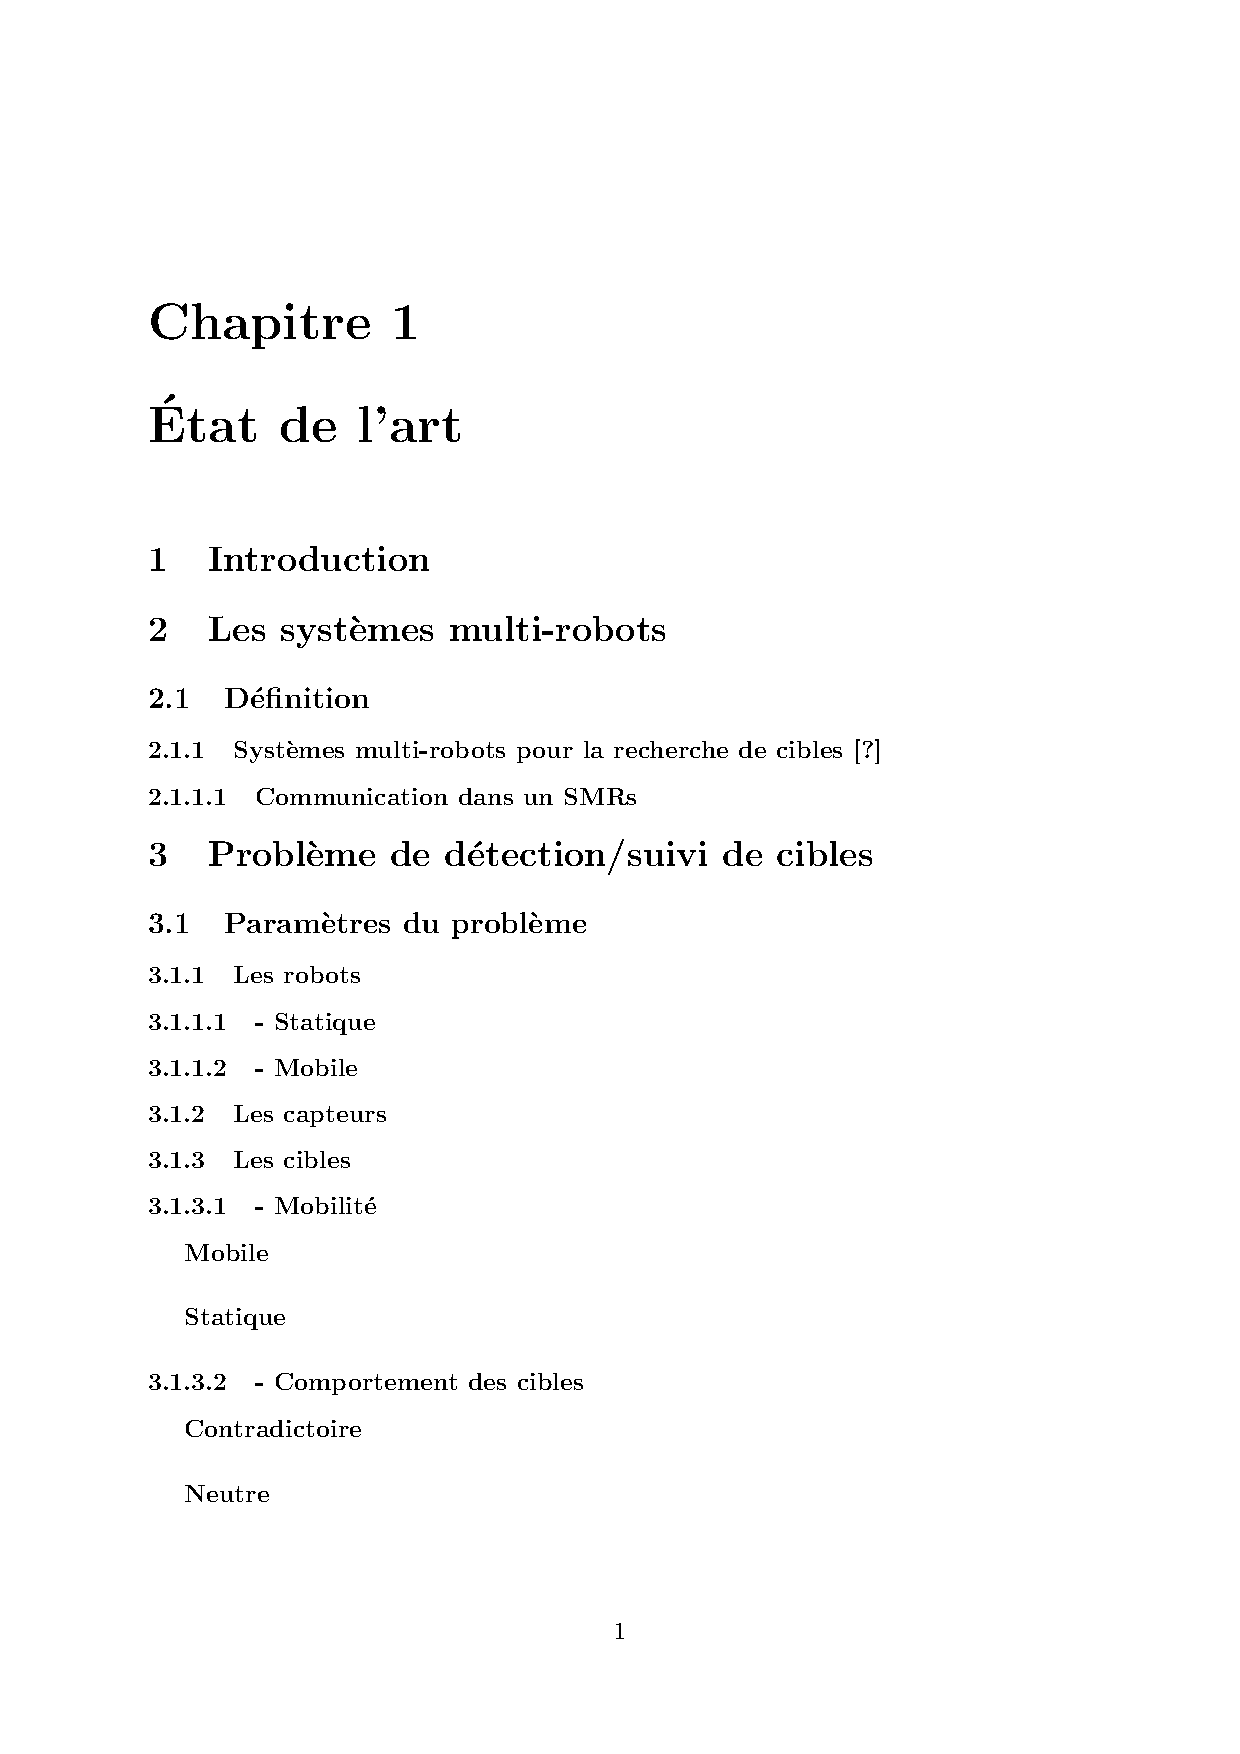
\includepdf{others/pagedegarde}	
 \let\cleardoublepage\clearpage

%	\begin{titlepage}
%		\begin{center}
%			
%			\vspace*{.06\textheight}
%			{\scshape\LARGE \univname\par}\vspace{1.5cm} 
%			\textsc{\Large Mémoire de Master}\\[0.5cm] 
%			\deptname\\[2cm]
%			
%			
%			\HRule \\[0.4cm] % Horizontal line
%			{\huge \bfseries \ttitle\par}\vspace{0.4cm} % Thesis title
%			\HRule \\[1.5cm] % Horizontal line
%			
%			\begin{minipage}[t]{0.4\textwidth}
%				\begin{flushleft} \large
%					\emph{Réalisation:}\\ \authorname % Author name - remove the \href bracket to remove the link
%				\end{flushleft}
%			\end{minipage}
%			\begin{minipage}[t]{0.4\textwidth}
%				\begin{flushright} \large
%					\emph{Sujet Proposé par:} \\
%					\supname % Supervisor name - remove the \href bracket to remove the link  
%				\end{flushright}
%			\end{minipage}\\[3cm]
%			
%			
%			
%			\examname
%			
%			\vfill
%			
%			
%			{\large \today}\\[4cm] % Date
%			%\includegraphics{Logo} % University/department logo - uncomment to place it
%			
%			\vfill
%		\end{center}
%	\end{titlepage}
%	


%----------------------------------------------------------------------------------------
%	ACKNOWLEDGEMENTS
%----------------------------------------------------------------------------------------

%
\thispagestyle{empty}
\renewcommand{\abstractname}{Remerciements}
\newenvironment*{remerciements}{%
	\renewcommand*{\abstractname}{Remerciements}
	\begin{abstract}
	}{\end{abstract}}

\addcontentsline{toc}{chapter}{Remerciements}


%\chapter*{Remerciements}
\begin{remerciements}
En tout premier lieu, je remercie ALLAH le tout-puissant, de m'avoir donné la force, l'audace, mais aussi la patience et le courage de persévérer et de mener à terme ce travail qui me tenait tant à cœur.

\vspace{0.2cm}

J'adresse mes sincères remerciements et toute ma gratitude à notre enseignante et promotrice Mme Habiba DRIAS, que ce soit pour les trois semestres d'enseignement durant lesquels elle n'a cessé de nous encourager, de nourrir nos esprits et de nous pousser à donner le meilleur de nous même, que pour son accompagnement tout au long de ces 4 mois de travail sur ce projet, de par sa disponibilité, ses conseils et orientations irremplaçables, mais aussi pour l'autonomie et la confiance qu'elle nous a accordée, j'ai grandi à vos côtés, merci.

\vspace{0.2cm}

J'adresse également, mes remerciements à Mr Mourad DAOUDI qui nous fait l'honneur de présider le jury de notre soutenance. Mes remerciements vont aussi à Mr Ilyes KHENNAK pour avoir accepté de faire partie de ce jury.

\vspace{0.3cm} 

Aussi, toute ma gratitude va à tous les enseignants de l'USTHB qui non seulement ont alimenté mon esprit et enrichi mon savoir mais aussi forgé mon caractère, mesdames: Khellaf, Aouat, Kadri, Amrouni(Kechid), Aliouane, Challal, Zemmouchi, Mehdi, Haddouche, Amrous, Bouziane, Ourahmoune, Boulekrinat, Gharbi, Zaouche, Chenait, Mahdaoui, Abdat, Hank, Baba Ali, Boughaci, Hadjazi, Bellala, Batoul, Mazouzi, Mankour, Rouaiguia, Hadouh, 
ainsi que messieurs: Guessoum, Azzoune, Kechid, Isli, Boukhelfa, Atif, Smaili, Abada, Djouadi, Djouama, Bouzeghoub, Bahloul, Laichi, Boudjaja, Daoudi, Amani, Ainouz.
Et tous les autres que je n'ai pas eus la chance d'avoir comme enseignant(e)s, j'ai pour ambition de revenir en cette faculté qui m'est chère, qui sait peut être nous serons collègues un jour inch'allah.

\vspace{0.2cm}
%%%%%%%%%%%%%%%%%%%%%%%%%%%%%%%%%%%%%%%%%%%%%%%%%%%

Aussi loin que remontent mes souvenirs, je me rappelle et me rappellerai toujours de tout ce que les deux êtres que j'admire le plus en ce monde et les plus chers à mes yeux ont fait pour moi et je ne les remercierai jamais assez qu'importe ce que je ferai. Papa, maman merci pour votre amour, votre présence, votre soutien, vos conseils, vos sacrifices, votre éducation et les valeurs que vous m'avez inculquées, tous vos efforts, votre patience, vos encouragements,  ... Et tant d'autres choses que je ne pourrais tous les citer. Merci je suis on ne peut plus fière de vous avoir et fière de ce que je suis aujourd'hui grâce à vous, j'espère vous avoir rendu fière à mon tour.

%%%%%%%%%%%%%%%%%%%%%%%%%%%%%%%%%%%%%%%%%%%%%%%%%%%

Je remercie chaleureusement mon grand frère pour ses encouragements, son support moral et pour m'avoir toujours guidé et inspiré. Je n'oublierai pas de remercier ma petite sœur qui a toujours cru en moi.
Ma pensée va également à ma tendre grand-mère qui ne cesse de prier jour et nuit pour ma réussite et toute ma famille qui m'ont soutenu tout le long de ce projet.

\vspace{0.2cm}

%%%%%%%%%%%%%%%%%%%%%%%%%%%%%%%%%%%%%%%%%%%%%%%%%%%%%%%%%%

Enfin, je remercie en général tous mes ami(e)s et camarades que je ne pourrais nommer un à un et en particulier mon amie et binôme Hassina Safaa MOULAI, pour leur appui et leur confiance qu'ils m'ont témoignée et pas seulement dans le cadre de ce travail mais durant tout mon cursus, du fond du cœur je vous souhaite à tous, que vos réussites s'enchaînent les unes après les autres.
Afin de n'oublier personne, à tous les intervenants de près ou de loin, je présente mes remerciements, mon respect et ma gratitude.
\end{remerciements}
\thispagestyle{empty}%

%\vspace{1.5cm}
%
%\setlength{\parindent}{0.5cm}
%\centering


\vspace{-0.3cm}
\begin{center}
\Large
\hspace{12.5cm}
\textbf{Naila}
\end{center}
%%\newpage
%\chapter*{Remerciements}


Je tiens à adresser mes remerciements au bon Dieu pour m’avoir donné le courage et patience de mener à terme ce modeste travail.\\

Je voudrais dans un second temps remercier, notre directrice de mémoire Professeur Habiba DRIAS, notre enseignante aussi durant notre formation, pour sa patience, sa disponibilité et surtout ses judicieux conseils, qui ont contribué à alimenter ma réflexion, ainsi que ces enseignements qui nous ont instruit de plus d'alimenter notre savoir sur plusieurs plans.\\

Je remercie également messieurs les membres du jury, Mr Mourad DAOUDI et Mr Ilyes KHENNAK d’avoir accepté d’examiner et de juger notre travail.\\


Je tiens particulièrement à témoigner une reconnaissance et gratitude envers tous nos professeurs qui ont contribué à notre formation particulièrement celle de master qui nous a formé, forgé notre caractère et nous a poussé à travailler davantage.\\


Un grand merci à tous mes amis qui ont été présents par leurs conseils et leur motivation tout au long de ce projet, particulièrement ma binôme Naila pour sa patience et son sérieux.\\

Enfin, mes plus chers remerciements vont à mes parents et membre de ma famille pour leur présence et encouragement et leur soutien inestimable et bien plus encore que je ne saurai citer.

%%\newpage
%
%
%%----------------------------------------------------------------------------------------
%%	DEDICATION
%%----------------------------------------------------------------------------------------
%
%%

\vspace*{\stretch{0.8}}
\begin{flushright}
 	\textit{Je dédie ce travail à la mémoire de mon grand père allah y rahmou,}\\
 	 \textit{à mes parents bien-aimés et à toute ma famille ainsi qu'à}\\
 	 \textit{toute l'équipe de Master SII 2017 - 2019.}\\
 	 \vspace{0.5cm}
 	\textbf{Naila}
\end{flushright}
\vspace*{\stretch{1}}


%%\newpage
%%\input{others/HassinaDedi}
%
%%\newpage
%
%%----------------------------------------------------------------------------------------
%%	ABSTRACT PAGE
%%----------------------------------------------------------------------------------------
%%
%%
\selectlanguage{french}
\begin{poliabstract}{Résumé}
	La frontière entre la fiction est la réalité devient chaque jour plus mince du aux évolutions technologiques qui ont émergé au fil des années. Les robots ne font plus partie de la science fiction seulement, ils se sont installé dans notre quotidien offrant de nouvelles capacités à l’Homme pour sa vie de tous les jours. 
	
	
	Les systèmes multi-robots ont conquis le monde de la recherche dans multiples domaine grâce à l'intelligence des robots qui est du à leur coopération lors de la planification des taches, c'est la raison pour laquelle plusieurs études se sont données comme but de les rendre de plus en plus performant robuste et efficace.
	
	L'un de leurs domaine d'application les plus récemment exploité est la recherche de cibles, c'est un problème qui consiste à maximiser le nombre de cibles trouvées dans une certaine zone ayant une superficie connue et des caractéristiques qui lui sont propre (présence d'obstacles,nombre de cibles, ..etc), la planification des actions des robots devient alors un défi faisant face à des contraintes liée aux caractéristiques de l'environnement.
	
	Notre projet consiste à apporter des solutions à la recherche de cibles  en adaptant des approches d'intelligence en essaim à cette thématique, communément appelées "métaheuristiques" ces approches n'ont pas encore été adapté sur ce type de problème et qui sont:  \textit{BSO et Multi-Swarm-BSO} s'inspirant de l'intelligence d'essaim d'abeilles. 
	\textit{EHO et ESWSA} basé groupe d'éléphants qui s'inspire de la mémoire individuelle des éléphants ainsi que l'intelligence des clans, elles vont devoir  trouver un nombre maximum de cibles en évitant les obstacles potentiellement présents sur l'environnement qui inconnu au préalable.
	\paragraph*{Mots clés:}
	Systèmes Multi-robots, Recherche de cibles, Évitement d'obstacles , Métaheuristiques, Intelligence en essaim, BSO ,EHO, ESWSA , BSO-Multi-Swarm.
	
\end{poliabstract}
\selectlanguage{english}
\begin{poliabstract}{Abstract}
	The borderline between fiction and reality is getting thinner every day due to technological developments that have emerged over the years. Robots are no longer just part of science fiction, they have become part of our daily lives, offering new abilities to Man for his everyday life.
	
	Multi-robot systems have conquered the world of research due to the cooperation that makes robots intelligent as a group. Several studies works toward improving them by making it more robust and efficient.
	
	Target search is one of their most recently exploited fields of application , it consists in maximizing the number of targets found in a certain area that we call environment, the planning of robot actions becomes a challenge facing constraints related to the characteristics of the environment.
	
	Our project consists in providing solutions for Target search problem by adapting swarm intelligence approaches, commonly called "metaheuristics" these approaches have not yet been adapted to this problem. The first two approaches :
	\textbf{BSO and Multi-Swarm-BSO} are inspired by the intelligence of a swarm of bees. 
	while the two last one \textbf{EHO and ESWSA} are elephant group based that draws inspiration from the individual memory of elephants as well as the intelligence of clans.
	this metaheuristics will aim to find a maximum number of targets by avoiding potentially present obstacles on the unknown environment.
	\paragraph{Keywords:} 	Multi-robots system,Target search, Obstacles avoidance , Metaheuristics, Swarm intelligence, BSO ,EHO, ESWSA , Multi-Swarm BSO.
\end{poliabstract}



%%\clearpage
%%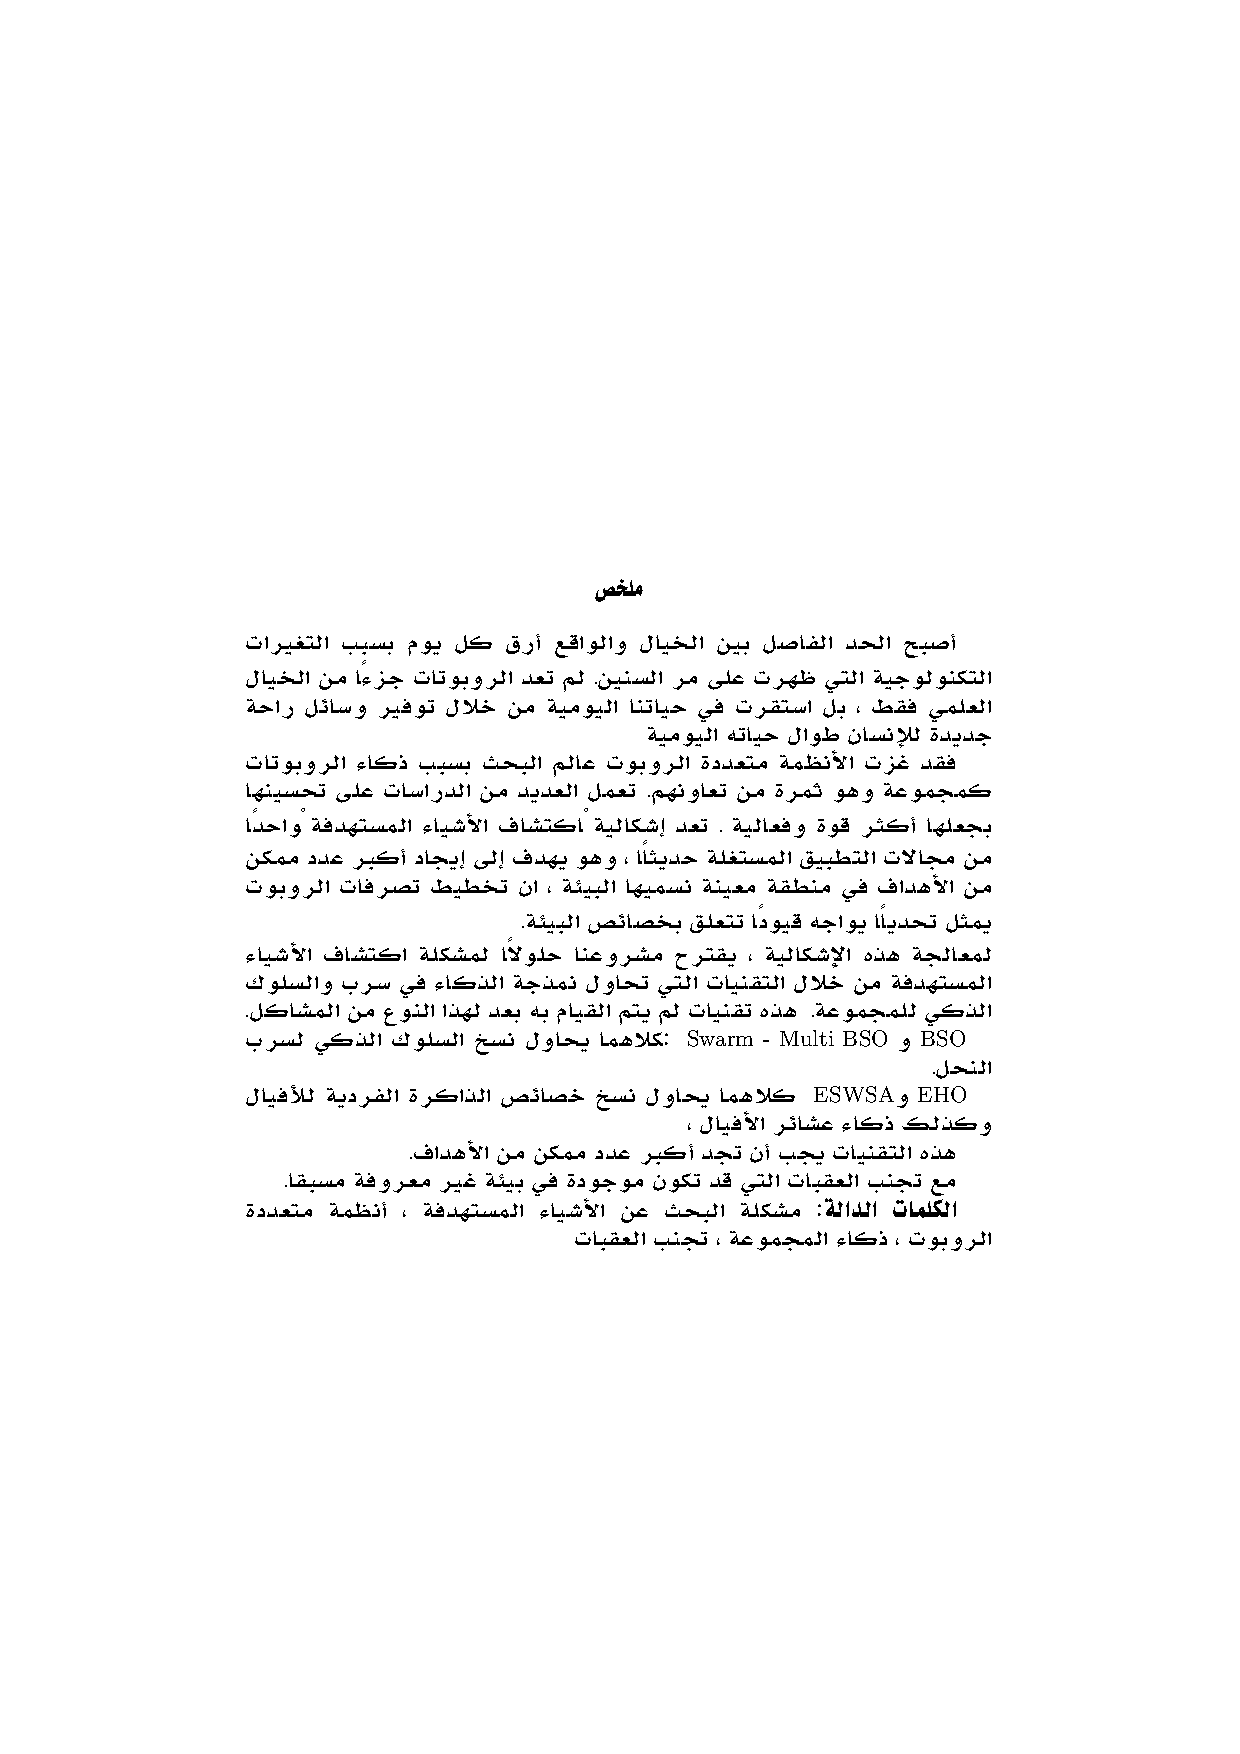
\includepdf{others/arabicabstract}
%%%
%%%----------------------------------------------------------------------------------------
%%%	LIST OF CONTENTS/FIGURES/TABLES PAGES
%%%----------------------------------------------------------------------------------------
%
\tableofcontents % Prints the main table of contents


\listoffigures % Prints the list of figures


\listoftables % Prints the list of tables
%
%%
%%	\listofalgorithmes
%%%	\clearpage
%%
%%%----------------------------------------------------------------------------------------
%%%	ABBREVIATIONS
%%%----------------------------------------------------------------------------------------
%%
\begin{abbreviations}{ll} % Include a list of abbreviations (a table of two columns)
	%\textbf{IA} & \textbf{I}nelligence \textbf{A}rtificielle\\
	%\textbf{IAD} & \textbf{I}nelligence \textbf{A}rtificielle \textbf{D}istribuée\\
	
	\textbf{PSO} & \textbf{P}article \textbf{S}warm \textbf{O}ptimization \\
	\textbf{GA} & \textbf{G}enetic \textbf{A}lgorithm\\ 
	\textbf{ACO} & \textbf{A}nt \textbf{C}olony \textbf{O}ptimisation\\
	\textbf{BA} & \textbf{B}ees \textbf{A}lgorithm\\ 
	\textbf{ABC} & \textbf{A}rtificial \textbf{B}ee \textbf{C}olony Optimisation\\
	\textbf{BFO} & \textbf{B}acterial \textbf{F}oraging \textbf{O}ptimisation\\
	\textbf{GSO} & \textbf{G}lowworm \textbf{S}warm \textbf{O}ptimisation\\
	\textbf{FA} & \textbf{F}irefly \textbf{A}lgorithm\\
	\textbf{DW} & \textbf{D}inamic \textbf{W}indow\\
	\textbf{SAT} & \textbf{S}atisfaction\\
	
	
	\textbf{FKD} & \textbf{F}iltre de \textbf{K}alman \textbf{D}istribué \\
	
	\textbf{FOA} & \textbf{F}ruit \textbf{F}ly \textbf{O}ptimization \textbf{A}lgorithm\\
	\textbf{MSCM} & \textbf{M}ulti-\textbf{S}cale \textbf{C}ooperative \textbf{M}utation\\
	
	
	\textbf{BSO} & \textbf{B}ee \textbf{S}warm \textbf{O}ptimization\\
	\textbf{EHO} & \textbf{E}lephant \textbf{H}erding \textbf{O}ptimization\\
	\textbf{ESWSA} & \textbf{E}lephant \textbf{S}warm \textbf{W}ater \textbf{S}earch \textbf{A}lgorithm \\
	\textbf{GA} & \textbf{G}énétique \textbf{A}lgorithme \\ 
	
	\textbf{Méta} & \textbf{M}étaheuristique\\ \textbf{Algo} & \textbf{A}lgorithme\\ 
	
	
\end{abbreviations}
%


%----------------------------------------------------------------------------------------
%	THESIS CONTENT - CHAPTERS
%----------------------------------------------------------------------------------------

\mainmatter % Begin numeric (1,2,3...) page numbering
\pagestyle{thesis} % Return the page headers back to the "thesis" style

% Chapter 0

\chapter*{Introduction générale} % Main chapter title
\addcontentsline{toc}{chapter}{Introduction}

\label{Introduction} % For referencing the chapter elsewhere, use \ref{Introduction} 
% Chapter 0


Une vague d'avancées technologiques a submergé le monde durant cette dernière décennie, l'intelligence artificielle est au centre de toutes les innovations étant par conséquent le sujet le plus actuel et un critère d'évaluation du développement des pays du monde.


Cet intérêt croissant a permis à des villes intelligentes de voir le jour ainsi que des voitures autonomes ou encore des robots sociaux comme Sophia \cite{sofia}.\\

Le développement connu par l'intelligence artificielle peut être expliqué par des besoins accrus et nécessaires de gain de temps, d'efforts et de mains d'œuvres humaines dans l'accomplissement de tâches quotidiennes.

Dans le but de participer à ce développement, les chercheurs ont essayé de proposer des solutions automatisant certaines tâches quotidiennes coûteuses en temps ou jugées dangereuses pour l'homme.
Les systèmes multi-robots font partie des innovations émergentes et solutions proposées pour répondre à ces besoins. Leur usage s'étale sur des domaines d'application des plus intéressants, allant de l'usage domestique au domaine militaire, passant par l'industrie ou encore le domaine de la santé. Ces multiples applications exploitent l'adaptabilité des robots qui sont capables de résoudre divers problèmes \cite{uses}.\\


Notons que la mobilité des robots est l'une de leurs capacités la plus convoitée, que ce soit dans l'assemblage et l'entreposage, le transport industriel, les équipements de nettoyage du sol  \cite{novel}, l'exploration de planète, la recherche et le secourisme des victimes dans une zone sinistrée ou encore la localisation de mines ou de bombes \cite{Dadgar2016}.

De plus, les systèmes multi-robots se caractérisent par leur coopération, celle-ci permet d'établir une meilleure planification des actions et comportements des robots face au monde qui les entoure pour aboutir à un but commun. 
\\
% Cette coopération  a pour but de simuler interactions et processus de raisonnement humain. D’ailleurs une équipe de robots, bien qu'ayant un comportement simple ou n'étant pas puissant individuellement peut compenser et surpasser ses limites grâce à la coopération \cite{Anderson2008}.\\

Ces systèmes multi-robots ont été particulièrement efficaces lorsqu'il s'agissait de problèmes de recherche ou détection, que ce soit dans des espaces connus ou inconnus. L'objectif consiste à localiser une ou plusieurs cibles se trouvant dans un certain espace qu'on appelle environnement. Une cible au sens large peut représenter des personnes perdues, des mines, de l'or, des puits de pétrole et bien plus encore.\\

La détection de cibles est un problème  complexe dont il découle un certain nombre de problématiques. On cite, l'optimisation des temps et efforts des robots à travers un choix adéquat de structure de coopération.  La conception d'un système d'évitement d'obstacles et de navigation fiable est primordial pour garantir des déplacements sans collisions au sein d'environnements inconnus, pouvant contenir des obstacles. Mais encore, les robots doivent adopter des stratégies de recherche intelligentes en raison de leur manque d'information sur l'environnement.\\
 


À travers ce travail, nous chercherons à proposer de nouvelles méthodes de résolution pour la détection de cibles en tentant d'apporter des améliorations au niveau des performances, c'est à dire qu'on vise à minimiser l'effectif (le moins de robots possibles) pour couvrir toute la zone de recherche, cela en trouvant le maximum de cibles.\\

 Notre contribution comportera une adaptation d'un système multi-robots aux quatre approches inspirées de l'intelligence en essaim, à savoir \textit{BSO} et \textit{Multi-BSO} qui sont basées sur le comportement des abeilles lors de la recherche du pollen, puis \textit{EHO} et \textit{ESWSA} qui sont inspirées de l'intelligence des éléphants en termes de communication et planification lors de la recherche d'eau et de nourriture. Un robot se comportera comme une abeille, un essaim d'abeilles ou un éléphant selon l'approche choisie.

Ces quatre approches devront être adaptées à une même modélisation du problème afin de permettre une comparaison effective des résultats obtenus. Pour cette même raison, la stratégie d'évitement d'obstacles sera exploitée et intégrée pour toutes nos méta-heuristiques.\\ 

Ce mémoire compte quatre chapitres organisés comme suit :

D'abord, une synthèse sur les maintes variantes du problème et tous les paramètres influant la direction qu'il peut prendre est présentée dans le chapitre 1.
Les algorithmes d'intelligence en essaim choisis pour l'élaboration de nos solutions sont décrits dans le chapitre 2.
Le chapitre 3 fera l'objet de la modélisation de notre problème et des stratégies d'évitement d'obstacles.
Le chapitre 4 comportera les deux premières contributions basées intelligence des essaims d'abeilles à savoir BSO et Multi-BSO. Deux autres contributions concernant deux algorithmes s'inspirant des éléphants qui sont EHO et ESWSA, seront présentées dans le chapitre 5.

L'efficacité des approches proposées sera validée à travers plusieurs expérimentations dont les résultats seront exhibés au chapitre 6. 
Enfin nous terminerons par une conclusion sur l'ensemble du travail effectué ainsi que des perspectives.









\let\cleardoublepage\clearpage
\chapter{Chapitre 1 : État de l'art} % Main chapter title

\label{Chapter1} % For referencing the chapter elsewhere, use \ref{Chapter1} 

%----------------------------------------------------------------------------------------

\section{Introduction}
La détection et le suivi de cibles englobent une large variété de problèmes décisionnels, tels que la surveillance, la recherche, les patrouilles, l’observation et la poursuite-évasion. Compte tenu du besoin croissant en effectif, en temps et en minimisation des coûts, de nombreuses applications ont été développées notamment dans des domaines comme le commerce et la défense.

Dans ce chapitre, nous nous attelons à fournir une synthèse sur les différents travaux inhérents à la recherche de multiples cibles dans un environnement inconnu et complexe. Au préalable, nous devons introduire certaines définitions et techniques propres à la nature des environnements auxquels nous aurons à faire face, d’autres concernant les méthodes de résolution. On finira par une conclusion dans laquelle nous situerons clairement la problématique traitée. 



\section{Problématique} 
\textbf{Pourquoi s'intéresser à la détection de cibles ?}\\

La détection de cibles est un problème intéressent dont la résolution apporte des avantages et gain de temps couvrant diverses besoins quotidiens qui s'étalent sur divers domaines.

Nous nous intéressons particulièrement à la recherche de mines anti-personnelles et bombes ainsi que la recherche de sources radioactives, car rien n’est plus important que la sécurité et la mise hors de danger de vies humaines.

Pour cela, nous aurons recours à des méthodes de résolution basées sur l’intelligence en essaim. Ces méthodes ont permis dernièrement de maintes avancées, jugées les plus adéquates comme technique de résolution.

De ce fait, nous aurons besoin de développer un système multi-robots où chaque robot se comportera comme une particule de l’essaim.

L’environnement inconnu est considéré en 2D, chaque robot n’a connaissance que du nombre de cibles recherchées, les bordures ou frontières de l’environnement de recherche ainsi que sa position initiale (position avant le début de la recherche).
Aussi l’environnement est complexe et englobe plusieurs obstacles, entravant son exploration.

Les positions des obstacles sont inconnues, c’est pourquoi les robots doivent être munis de capteurs adaptés à leur stratégie d’évitement d’obstacles.
Les cibles (mines / sources de radiation) dont les positions sont inconnues, émettent un signal que les robots sont capables de réceptionner via leurs capteurs.

La validation du système sera effectuée par des expérimentations sur des environnements dont les positions des obstacles, cibles et des robots sont générées aléatoirement. Cela conformément à la procédure présentée dans des travaux récents.





\section{Paramètres du problème}
Plusieurs paramètres entrent en jeu concernant le problème de recherche de cibles, donnant lieu à une arborescence de sous-classes de problèmes (voir figure \ref{classesProb}), qui se diffèrent par les techniques de résolutions adaptées.

\begin{center}	  
	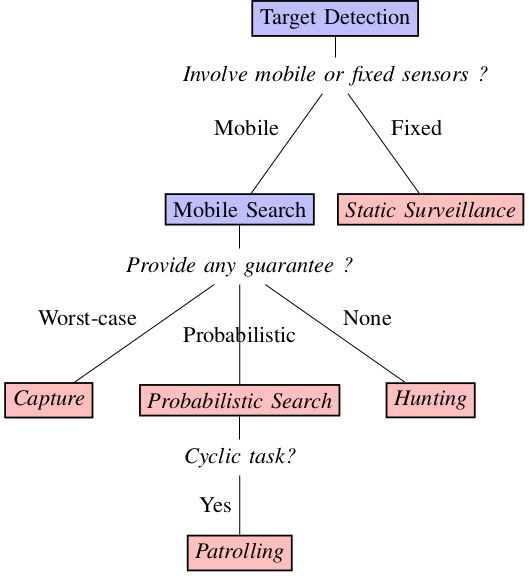
\includegraphics[width=0.4\textwidth]{../Figures/targetdetection.png}%
	\vspace{-0.1 cm}
	\captionof{figure}{Schéma résumant les classes de problèmes de détection de cibles \cite{surv2}.}\label{classesProb}%
\end{center}

Nous distinguons quatre types de problèmes : 
\begin{itemize}
	\item[$\bullet$] \textbf{La surveillance statique} implique l’utilisation de robots fixes dans un environnement connu afin d’entièrement le couvrir pour y détecter les cibles \cite{surv2}. 
	
	
	
	\item[$\bullet$] \textbf{La capture} a pour but de capturer toutes les cibles présentes dans un environnement connu. Seules les positions initiales des cibles ne sont pas connues par le(s) poursuiveur(s) \cite{surv2}. La figure \ref{capture} illustre un exemple de capture.
	\begin{center}	  
		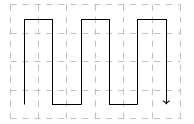
\includegraphics[width=0.27\textwidth]{../Figures/capture.png}%
		\vspace{-0.1 cm}
		\captionof{figure}{Exemple de capture \cite{surv2}.}\label{capture}%
	\end{center}
	
	
	
	\item[$\bullet$] \textbf{La patrouille} a une formulation proche de celle de capture, mais avec un aspect cyclique. Autrement dit la zone n’est pas couverte qu’une seule fois, mais plusieurs fois \cite{surv2}, comme le montre la figure \ref{patrou}.
	\begin{center}	  
		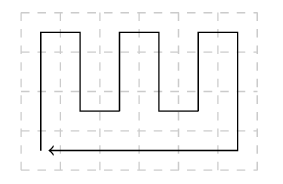
\includegraphics[width=0.3\textwidth]{../Figures/patrolling.png}%
		\vspace{-0.1 cm}
		\captionof{figure}{Exemple de patrouille \cite{surv2}.}\label{patrou}%
	\end{center}
	
	\item[$\bullet$] \textbf{La chasse} s’attaque à la détection de cibles sans aucune garantie. C’est-à-dire qu’on suppose qu’on ne connaît ni les positions initiales des cibles ni l’environnement de recherche \cite{surv2}. \\
\end{itemize}



À partir de la formulation de la problématique et des classes de problèmes présentées ci-dessus, on peut clairement situer notre contribution, qui s'inscrit dans le cadre des problèmes de type  \textbf{Chasse}. 

Dans ce qui suit nous dériverons les paramètres du problème les plus pertinents :


\subsection{Les systèmes multi-robots (SMRs)}

\subsubsection{Définition}
Un système multi-robots est un groupe de robots mobiles autonomes ayant un objectif ou un ensemble de tâches communes, ces robots ont la capacité de communiquer et se coordonner afin d'atteindre leur objectif \cite{SMR1}. 

Les robots mobiles se déplacent durant la recherche selon une stratégie visant à aboutir à des solutions optimales.

Il est important de souligner que le mode de mobilité des robots influence fortement la résolution du problème (vision, vitesse, agilité du mouvement) \cite{surv1}.



\subsubsection{Caractéristiques des SMRs \cite{surv1}}
Les systèmes multi-robots se caractérisent par multiples aspects qui font leur force, à commencer par l'exécution des tâches en parallèle, ainsi qu’une couverture d'une plage assez importante de l'espace de recherche. D'autres particularités des SMRs spécifiques aux essaims de robots existent, telles que:
\begin{itemize}
	\item[$\bullet$]\textit{La robustesse}, qui offre une tolérance aux pannes.
	
	\item[$\bullet$]\textit{la flexibilité} permet une rapide adaptation aux nouvelles exigences et différents environnements (favorisée par la redondance et la simplicité des comportements des robots).
	
	\item[$\bullet$]\textit{l'évolutivité} qui est la capacité à fonctionner avec un nombre plus grand ou plus petit de robots sans impact considérable sur la performance.
\end{itemize}

\subsubsection{Système de communication \cite{surv2}}
Deux types de systèmes sont les plus répandus: centralisés et décentralisés, ils sont choisis selon le besoin et les critères recherchés.


\begin{itemize}  
	\item[$\bullet$] \textbf{Les systèmes centralisés}, sont plus aptes à fournir une optimalité globale. Cependant, ils sont souvent confrontés à de fortes contraintes du  monde réel, d’où la nécessité d'une connectivité totale dans de nombreuses situations.
	
	\item[$\bullet$] \textbf{Les systèmes décentralisés}, quant à eux fournissent des solutions jugées sous-optimales. Par contre, ils sont plus robustes et plus flexibles de par leur adaptation aux environnements dynamiques ce qui leur permet d'aboutir à des performances intéressantes.
\end{itemize}


\subsubsection{Comportement des robots \cite{surv2}}
Les robots peuvent s'approprier deux types de comportements, soient:

\begin{itemize} 
	\item[$\bullet$] \textbf{Indépendant}, chaque robot est responsable d'un certain nombre de tâches à exécuter.
	
	\item[$\bullet$] \textbf{Coopératif}, chaque décision ou action est diffusée à toute l'équipe. Ce mode coopératif peut être explicite, consistant à influencer un robot par une communication directe, ou bien implicite, qui est une  prise de décision indépendante selon les informations individuellement recueillies.
\end{itemize}


\subsection{Les capteurs}
Selon l'environnement à explorer, le besoin en types de capteurs diffère, que ce soit pour reconnaître les cibles, détecter les obstacles afin de les éviter ou reconnaître les autres robots.

Parmi la panoplie des capteurs existants, on trouve : les caméras, les infrarouges, les capteurs lasers (distance), les capteurs à ultrason, la kinect, les capteurs de pression, les capteurs de gaz, GPS, ...etc \cite{capteur} qui sont les plus utilisés. Le choix des capteurs consiste à trouver le meilleur compromis entre coût et efficacité selon les contraintes imposées. 

\subsection{Les cibles}
Le nombre de cibles est un paramètre fixé pour un environnement donné. Les problèmes \textbf{mono-cible} consistent à trouver la position d'une cible particulière dans l'environnement. En revanche, les problèmes \textbf{multi-cibles} visent à maximiser le nombre de cibles trouvées. 

Pour le problème de recherche ou détection, les cibles possèdent des positions inchangées dans l'environnement durant toute la recherche 
\cite{surv1}.\\

De plus, il est toujours supposé que les cibles émettent des radiations, sons, ondes, lumières, odeurs ou autres, qui sont maximales aux alentours de la cible  s'estompant graduellement en s'éloignant de celle-ci. L'étendue du champ d'émission de ces cibles est aussi un paramètre qui influe directement l'efficacité des algorithmes de résolution.

\subsection{L'environnement \cite{surv2}}
L'environnement est l'espace de recherche où évoluent les cibles et interviennent les robots comme fouilleurs. Il est décrit comme \textbf{connu} lorsqu’une carte est mise à disposition et \textbf{inconnu} lorsqu'on manque d'informations globales, n'ayant connaissance que de ses bordures. Ces environnements peuvent être des:

\begin{itemize} 
	\item[$\bullet$] \textbf{Environnements simples}, c'est-à-dire sans obstacles ne contenant aucune contrainte susceptible de bloquer la vue ou la mobilité des robots.
	
	\item[$\bullet$] \textbf{Environnements avec obstacles ou complexes}, Ceux-ci contenant des obstacles, contraignants ainsi les robots dans leurs déplacements et leurs perceptions, les poussant parfois à changer de trajectoire.
\end{itemize}

\subsection{Les obstacles}
Les obstacles sont des contraintes supplémentaires dans le processus de recherche de cibles. Divers types d'obstacles existent, citons les obstacles fixes et mobiles, les obstacles franchissables mais entravant la vue ou encore les obstacles empêchant uniquement le passage sans obstruer la visibilité des robots, ... etc \cite{surv2}.\\

La présence d'obstacles dans les environnements de recherche impose aux méthodes de résolution une prise en considération d'une stratégie d'évitement d'obstacles, pour cela nombreuses sont les stratégies existantes.

Elles s'appuient sur les informations fournies par les capteurs embarqués afin d'orienter les robots à chaque laps de temps pour une réaction en temps réel \cite{Sara}. 





%\newpage


\section{Travaux connexes}
Plusieurs approches ont été exploitées pour la résolution du problème de détection de cibles dans des environnements inconnus, nous citons à titre d'exemple:

\subsection{Les algorithmes anti-regroupements \cite{Miao2010}}
Souvent appliqués aux problèmes de type "chasse", ces algorithmes imitent le comportement social des animaux solitaires (tigre, araignée, ...). Ils se basent sur trois principales règles, soient:

\begin{itemize}
	\item[$\bullet$] La prévention des collisions : en s'éloignant des obstacles les plus proches et en respectant une distance de sécurité.
	
	\item[$\bullet$] La décentralisation : en tentant de se séparer de ses voisins.
	
	\item[$\bullet$] L'égoïsme : si aucune des deux situations précédentes ne se produit, chaque robot choisit la direction permettant de maximiser ses propres gains.
\end{itemize}


\subsection{Approche des champs de potentiel \cite{surv2}}
Dans cette approche on considère deux vecteurs de forces locales qui influencent les mouvements des robots telles que, les cibles proches émettent des forces attractives vers elles, tandis que les robots proches émettent des forces répulsives éloignant ainsi les autres robots. L'algorithme de Parker pour le contrôle distribué A-CMOMMT est inspiré des champs de potentiels \cite{Parker2002}.

\subsection{Approches basées intelligence en essaim}
L'intelligence  en essaim  et les méta-heuristiques ont été très exploitées pour ce type de problème grâce à la facilité des opérations stochastiques qui les distinguent des autres techniques. Leur force majeure est l'inspiration des  comportements d'espèces ou phénomènes naturels \cite{robotMeta}.\\

PSO, GA, ACO, BA, ABC, BFO, GSO et FA sont les techniques de méta-heuristiques les plus utilisées revenant souvent dans la littérature avec des améliorations et contributions apportées par les auteurs \cite{surv1}. 

Quant aux travaux récents on trouve :

\subsubsection{BSO (Bee Swarm Optimization) (2013)}
Une variante de l’algorithme Bee Swarm Optimization inspirée du comportement des abeilles dont les auteurs sont Hannaneh Najd Ataei, Koorush Ziarati et Mohammad Eghtesad \cite{BSO2013} comporte trois types d’abeilles (abeilles butineuses, abeilles éclaireuses, abeilles spectatrices) chacune possède sa propre fonction de mise à jour de ses positions.\\	

Cette variante a montré de meilleures performances que la version classique de PSO.
Suite à des expérimentations sur un ensemble d’environnements aléatoires, il a été prouvé que cette approche de BSO peut être 50,6\% plus efficace que PSO.

Mais elle n’a été testée que sur des environnements mono-cibles. De plus, la fonction objectif utilisée s’appuie sur  la distance euclidienne entre les robots et la cible, or que les positions des cibles sont supposées inconnues.

\subsubsection{A-RPSO}
A-RPSO (Adaptative Robotic Particule Swarm Optimization) est une technique basée essaim proposée par les auteurs M. Dadgar, et al., où chaque particule représente un robot. La contribution de l’auteur par rapport à un PSO classique est l’ajout d’une stratégie d’évitement d’obstacles incluse dans l’équation de déplacement, ainsi qu’une mise à jour des paramètres classiquement constants comme le poids d'inertie de façon dynamique,  dite adaptative.\cite{Dadgar2016}.



Ces modifications ont eu comme objectif d’éviter les optimaux locaux, mieux contrôler et adapter l’allure des robots lors du rapprochement des cibles et des obstacles. La technique a été testée sur un simulateur 2D créé par les auteurs, elle reste proche d’une modélisation d’une grille virtuelle bidimensionnelle.  


\subsubsection{MFSO (Multi-swarm hybrid FOA-PSO)}
Un nouvel algorithme multi-essaim hybride (MFPSO) basé sur FOA (Fruit Fly Optimization Algorithm) et PSO (Particule Swarm Optimization) pour la recherche d’une cible dans des environnements inconnus a été présenté par les auteurs, Hongwei Tang, Wei Sun, Hongshan Yu, Anping Lin, Min Xue et Yuxue Song \cite{novel}. Cette nouvelle méta-heuristique se singularise par les avantages suivants : \\

\begin{itemize}
	\item [$\bullet$] Parallélisme grâce à un coefficient adaptatif.
	
	\item[$\bullet$] Présence de stratégies contournant la convergence prématurée grâce à l'indépendance des essaims de robots.
	
	\item[$\bullet$] Mécanisme d'évacuation (MSCM) comme stratégie d'évitement d'obstacles.\\
\end{itemize}

Les nombreuses expériences effectuées pour le mode mono-cible sur MFPSO prouvent qu’il surpasse de manière significative les autres approches (dont A-RPSO et RPSO), en termes de nombre d’itérations et taux de réussite, dans la plupart des cas.
 
Par contre, le champ d’émission de la cible est inconnu, or comme mentionné plus haut, ce paramètre influence la difficulté du problème.
 
Les tests effectués comportent le cas du mono-cible seulement, ce qui implique que le comportement et l’efficacité de cet algorithme dans des environnements multi-cibles sont inconnus. 

Aussi, le champ de vue des robots a été fixé par les auteurs à une valeur de dix pixels durant toutes les expérimentations. 

Enfin, les auteurs utilisent une fonction objectif qui manipule la distance $ Dist \left( x^{t}_{i} \right)$ entre les robots et la cible. Cependant, la position de la cible est supposée inconnue. C’est pourquoi cette distance au lieu d’être directement utilisée comme fonction objectif elle a servi à calculer une estimation des signaux émis par la cible. 





\section{Conclusion}
Ce chapitre nous a permis de décortiquer les différentes variantes du problème de détection de cibles ce qui nous a permis de déduire que notre travail visera à proposer une solution au problème de \textit{Chasse}.

 Tous les paramètres nécessaires pour clairement définir notre problème et aboutir à une bonne modélisation, ont été explicitement exposés.
Notre méthode de résolution est basée intelligence en essaim, d’où la nécessité d'éclaircir certains aspects incontournables relatifs aux approches choisies dans le chapitre suivant.

\let\cleardoublepage\clearpage
% Chapter 2
\chapter{Chapitre 2 : Intelligence en essaim : BSO, EHO, ESWSA et GA} % Main chapter title

\label{Chapter2} % For referencing the chapter elsewhere, use \ref{Chapter1} 

%----------------------------------------------------------------------------------------


\vspace{-0.5cm}
\section{Introduction}
Dans ce chapitre nous allons présenter les outils intelligents de résolution pour notre problématique. Ces derniers consistent en des méta-heuristiques inspirées de l'intelligence collective des animaux et insectes, autrement dit l’intelligence en essaim.

Nous commencerons par introduire les algorithmes basés intelligence en essaim et leurs principaux paramètres, suivis d'un décryptage des trois approches choisies pour notre étude, à savoir :
\begin{itemize}
	
	\item Bee Swarm Optimization (BSO) qui est un algorithme de résolution s'inspirant de l'intelligence collective du comportement des abeilles lors de la recherche de nourriture. BSO a fait ses preuves face à de nombreux problèmes d'optimisation combinatoire (le problème de satisfiabilité SAT, le problème du voyageur de commerce, ...etc.).
	
	\item Elephant Herding Optimisation (EHO) et Elephant Swarm Water Search Algorithm (ESWSA), tous deux des algorithmes inspirés du comportement des éléphants en groupe.
	
	\item On verra aussi l'algorithme génétique (GA) dans sa version GA incrémental.
\end{itemize}

On clôturera ce chapitre par les motivations qui nous ont poussées à choisir ces algorithmes intelligents comme méthodes de résolution pour la détection de cibles.


\section{Les algorithmes basées intelligence en essaim}
Swarm Intelligence ou l’intelligence en essaim étudie le comportement coopératif entre les espèces naturelles. C’est un domaine prometteur de l'intelligence artificielle dont le principe de base repose sur l'observation par la nature des phénomènes intelligents et surtout des comportements de groupe chez les animaux.

Une approche ou méthode basée intelligence en essaim est également considérée comme une méta-heuristique. Elle suit un schéma d'algorithme évolutif, dicté par la simulation de l'évolution des espèces naturelles \cite{courshabiba}.
\\

Les méta-heuristiques sont des approches génériques qui visent à proposer des solutions à des problèmes complexes, en employant une certaine stratégie d'exploration de l'espace de recherche appelée \textbf{espace des solutions}. Ce dernier comporte toutes les solutions possibles au problème. Ces \textbf{solutions} sont ensuite filtrées grâce à une \textbf{fonction objectif} permettant de les ordonner selon leur optimalité \cite{courshabiba}.\\

La figure \ref{metas} montre qu’il existe deux catégories principales de méta-heuristiques. Les méta-heuristiques basées sur une solution unique, telles que, la recherche tabou (TS)  \cite{aouatTS}, recuit simulé, la recherche locale guidée (GLS) \cite{habibaGLS}, ...etc, et les méta-heuristiques basées population comme l'algorithme génétique (GA) \cite{kechidGA} ou une de ses extensions, Les algorithmes mémétiques  (MA) \cite{habibaMA}, la recherche par dispersion (SS) \cite{habibaSS-GA}, l'algorithme Bat (BA) \cite{boukraBA-ACO,habibaBA2}, les colonies de fourmis (ACS)  \cite{habibaACO}, l'algorithme d'optimisation par essaim de particules (PSO) \cite{habibaPSO}, l'algorithme des lucioles FFA (Firefly algorithm) \cite{habibaFAA}, l'essaim d'abeilles à savoir BSO (Bee Swarm Optimization) \cite{habibaBSO1,kechidBSO}, ABSO (Advenced Bee Swarm Optimization) \cite{habibaABSO}, ou encore ABC (Artificial Bee Colony) \cite{boukraABC} etc.

Les algorithmes basés intelligence en essaim peuvent être vus comme des méta-heuristiques basées population \cite{courshabiba}.

Ces nombreux travaux ont été développés au sein du laboratoire de recherche en l'intelligence artificielle LRIA \footnote{https://www.lria.usthb.dz/}.

\noindent
\begin{center}	  
	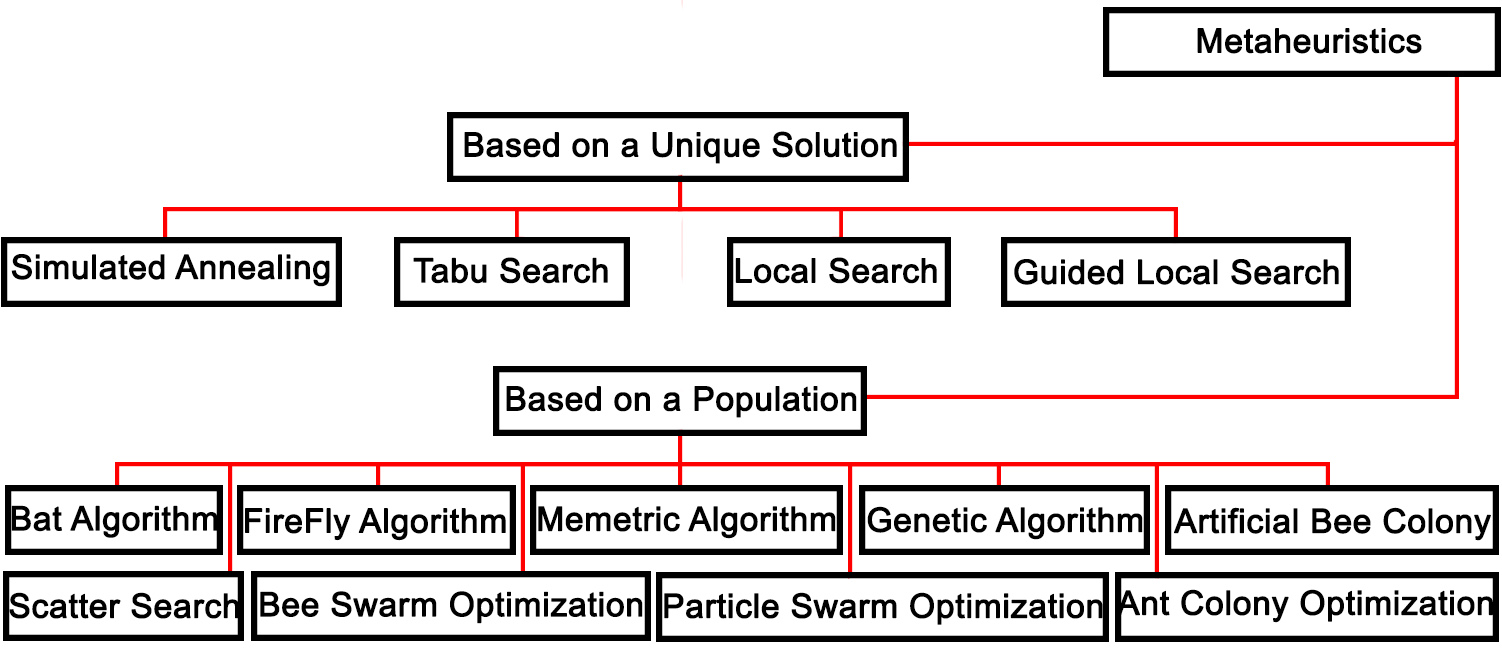
\includegraphics[width=0.9\textwidth]{metagraph.jpg}%
	\vspace{-0.1 cm}
	\captionof{figure}{Classification des méta-heuritiques}\label{metas}%
\end{center}


Étant donné l'efficacité et la simplicité des méta-heuristiques, on va s'intéresser de plus près à BSO, EHO, ESWSA et GA qui sont des méta-heuristiques basées population ayant connu un large intérêt et succès.

\section{Bee Swarm Optimization \cite{Drias}}

\subsection{Inspiration des abeilles}
De nombreuses études biologiques se sont intéressées aux comportements et à la psychologie des abeilles afin de décortiquer leurs méthodologies et stratégies de recherche du nectar ainsi que leur façon de communiquer les informations concernant leurs trouvailles.

L'une des expériences les plus connues sur les abeilles, est celle de Seeley, Camazine et Sneyd en 1991 \cite{Seeley}, elle a abouti sur les quelques caractéristiques suivantes :
\\

\begin{itemize}
	
	\item[$\bullet$] la catégorie d'abeilles \textit{"travailleuses"} est celle qui se charge de trouver la nourriture ("Scout bee"). Les abeilles reviennent à la ruche en ramenant un peu de leurs récoltes.
	
	\item[$\bullet$]Les abeilles ont tendance à privilégier les régions qui regorgent de nourriture aussi lointaines soient elles aux zones moins riches en pollen, mais à proximité de la ruche.
	
	\item[$\bullet$] L'abeille ayant trouvé la meilleure région en termes de nourriture effectuera la danse la plus rigoureuse, ce qui guidera l'essaim vers la meilleure région.
	
	\item[$\bullet$] La danse (mouvement circulaire) est le moyen de communication entre les abeilles, elle englobe les informations concernant la quantité, la direction et la distance entre la ruche et la région où se trouve la nourriture.
\end{itemize}

\subsection{Analogie entre le comportement des abeilles et BSO}
BSO est entièrement inspirée du comportement des abeilles pour la recherche du pollen, ci-dessous le tableau \ref{analogieBSO} fait l'analogie entre le comportement des abeilles travailleuses et leurs représentations simplifiées dans BSO :\\

\begin{table}[h]
	\centering
	\begin{tabular}{|p{7cm}|p{7cm}|} 
		\hline
		
		\textbf{Essaim d'abeilles} & \textbf{BSO}\\ 
		
		\hline
		Une abeille éclaireuse est envoyée dans un champ de fleurs et se positionne sur une fleur aléatoirement. &  
		Une solution est générée aléatoirement à partir de l'espace des solutions, elle est ensuite affectée à l'abeille de référence. \\ 
		\hline
		Les abeilles s'orientent vers les champs de fleurs à la recherche de quantité de nourriture (pollen). & Les abeilles artificielles se déplacent dans l'espace des solutions à la recherche de bonnes solutions.\\
		\hline
		Les abeilles se dispersent autour de la zone indiquée par l'abeille éclaireuse pour couvrir au mieux le champ de fleurs. &  La diversification est basée sur le Flip. Ce dernier permet la génération d'un certain nombre de solutions à partir de la solution de référence. \\ 
		\hline
		%			\end{tabular}
		%\end{table}
		%\begin{table}[h]
		%	\centering
		%	\begin{tabular}{|p{7cm}|p{7cm}|} 
		%		\hline	
		Chaque abeille procède à une recherche locale dans sa zone d'atterrissage. & 
		Chaque abeille porteuse d'une solution effectue une recherche locale, ce processus est appelé \textit{"intensification"}.  \\
		\hline
		Chaque zone de fleurs est évaluée selon la quantité de pollen qui s'y trouve. &  Chaque solution est évaluée selon la fonction objectif.\\ 
		\hline
		Chaque abeille se rappelle de la fleur source ayant la plus grande quantité de pollen ainsi que l'endroit où elle se trouve. Elle se met à danser juste au-dessus pour en informer l'essaim. &  Chaque abeille sauvegarde sa meilleure solution locale dans une table appelée \textit{Table Dance}.\\ 
		\hline
		La vigueur de la danse de l'abeille est proportionnelle à la richesse et quantité de nourriture trouvée.
		& 	La sélection d'une solution de la table \textit{Dance} se base sur un critère de qualité. Toutes les abeilles sont mises au courant de la meilleure solution actuelle. \\
		\hline
		En cas de recherche non-fructueuse, les abeilles explorent d'autres zones distantes & en cas de stagnation de la recherche, la solution la plus diverse de la table \textit{Dance} est sélectionnée comme solution de référence. \\ 
		\hline
		%\bottomrule
	\end{tabular}
	\captionsetup{width=1\linewidth}
	\caption{Analogie entre les caractéristiques des essaims d'abeilles et BSO.}
	\label{analogieBSO}
\end{table}

\newpage

\subsection{Paramètres et fonctions}
BSO est caractérisée par plusieurs paramètres empiriques, qui sont : 
\begin{itemize}
	\item[$\bullet$] \textbf{nbrBee} : le nombre d'abeilles de l'essaim.
	\item[$\bullet$] \textbf{Flip} : la fréquence d'inversement.
	\item[$\bullet$] \textbf{MaxChance} : le nombre de chances maximal. 
	\item[$\bullet$] \textbf{MaxItération} : le nombre d'itérations maximal.\\
\end{itemize}

\textbf{Sref:} La solution de référence est initialisée aléatoirement au début de la recherche, puis mise à jour selon les étapes de BSO, par la meilleure solution en termes de qualité ou de diversité.\\ 

\textbf{Flip:}
C'est un paramètre qui détermine le nombre de variables à inverser au niveau de la solution de référence (Sref) afin d'obtenir de nouvelles solutions. $\frac{n}{flip}$ représente ainsi la distance qui sépare les nouvelles solutions de \textit{Sref}, \textit{n} étant la taille de la solution. \\

\textbf{Détermination des zones de recherche:}
l'application du \textit{Flip} sur une solution de référence génère un ensemble de solutions équidistantes de \textit{Sref}, formant un cercle autour d'elle.\\


\textbf{Recherche locale:}
Chaque abeille effectue une recherche locale à partir de la solution qui lui est affectée afin d’évaluer les solutions voisines en ne gardant que la meilleure.\\

\textbf{MaxChance:}
Chaque solution possède un nombre de chances maximal pour être choisie comme solution de référence à chaque itération.\\


\textbf{Table dance:}
La table \textit{"Dance"} est le répertoire commun à toutes les abeilles de l'essaim pour y inscrire leurs meilleures solutions locales.\\

\subsection{Pseudo-code BSO}
\vspace{-0.2cm}
\begin{algorithm}[H]
	\TitleOfAlgo{BSO}
	\vspace{-0.2cm}	
	\xdash[13.5cm]
	
	\SetAlgoLined
	\DontPrintSemicolon
	\KwIn{$MaxIteration,Flip,Maxchances,Optimale,nombre d'abeilles$}
	\KwOut{$meilleureSolution$ : la meilleure solution trouvée}
	
	\SetKwFunction{solutionAleatoire}{solutionAléatoire()}
	\SetKwFunction{Insertion}{Insertion}
	\SetKwFunction{DeterminationDesZonesDeRecherche}{DeterminationDesZonesDeRecherche}
	\SetKwFunction{rechercheLocale}{rechercheLocale}
	\SetKwFunction{MeilleureDeDance}{MeilleureDeDance}
	
	\tcc{génération aléatoire de la solution de reference.}
	$Sref \gets$ \solutionAleatoire\;
	$meilleureSolution \gets Sref$\;
	
	\tcc{Tant que le nombre d'itérations maximal n'est pas atteint et la solution optimale n'est pas trouvée réitérer}
	\While{$\neg$  ($MaxIteration$ \textbf{or} $Optimale$) }{
		\tcc{Insertion de la solution de référence dans la liste Tabou}
		\textbf{\Insertion($listeTabou$,$Sref$)}\;
		\tcc{Affectation des zones de recherche aux abeilles}
		$abeilles \gets$
		\DeterminationDesZonesDeRecherche($Sref$)\;
		
		\ForEach{$abeille \in abeilles$}
		{
			\tcc{Effectuation d'une recherche locale}
			$solutionLocale \gets$ \rechercheLocale($abeille$)\;
			\tcc{Evaluation et insertion de la meilleure solution locale dans la table Dance.}
			\Insertion($Dance$,$MeilleuresolutionLocale$)\;
		}
		\tcc{Sélection de la meilleure solution de la table Dance.}
		$Sref \gets $\MeilleureDeDance($Dance$)\;
		\If{$sRef > meilleure$ }{
			\tcc{Sauvgarde de la nouvelle meilleure solution.}
			$meilleureSolution \gets sRef$\;
		}
	}
	\Return $meilleureSolution$\;
	\caption{BSO Générique}
\end{algorithm}

\textbf{ }


\begin{function}[H]
	\TitleOfAlgo{DéterminationDesZonesDeRecherche}
	\vspace{-0.2cm}		
	\xdash[13.5cm]
	
	\SetAlgoLined
	\DontPrintSemicolon
	\KwIn{$Flip$ : fréquence d'inversement}
	\KwOut{$ensemble\_K\_solutions$ : ensemble de K solutions}
	$h \gets 0$\;
	
	\SetKwFunction{Inverser}{Inverser}
	
	
	\While{$taille(espace_{recherche}) < k$ \textbf{and} $h < Flip $}
	{ $s \gets Sref$; 	$p \gets 0$\;
		\tcc{Inversion partielle de la solution, à une fréquence : flip}
		\Repeat{$Flip*p+h>n$}
		{
			
			$s \gets$ \Inverser($s,s[Flip*p+h]$)\;
			$p \gets p + 1$\;
			
		}
		\tcc{Insertion de la solution générée dans la liste de solutions}
		$ensemble\_K\_solutions \gets ensemble\_K\_solution\cup$ $\{s\}$\;
		$h \gets h + 1$\;
	}
	
	\Return $ensemble\_K\_solutions$\;
	
	\caption{DéterminationDesZonesDeRecherche()}
	
\end{function}






%\newpage

\section{EHO \& ESWSA : Deux algorithmes basés essaim d'éléphants}
\subsection{Inspiration des éléphants}
Les éléphants sont des mammifères sociaux qui présentent des structures sociales complexes ayant une multitude de particularités surprenantes.


Dans un premier temps, on se contentera d'exhiber les caractéristiques individuelles suivantes \cite{EHO1} :


\begin{itemize}
	
	\item[$\bullet$] Bonne mémoire.
	\item[$\bullet$] Font preuve d'une intelligence avancée (reconnaissance de soi, la conscience de soi).
	\item[$\bullet$] Capacité d'apprendre et de distinguer plusieurs discriminations visuelles et acoustiques.
	\item[$\bullet$] Capacité à utiliser et manipuler des outils de la vie réelle.
	\item[$\bullet$] Possession de systèmes de détection et de communication très avancés.
\end{itemize}
\textbf{ }\\
\textbf{ }
Quant aux caractéristiques de groupe, nous citons \cite{EHO2} :


\begin{itemize}
	\item[$\bullet$] Un groupe d'éléphants est composé de plusieurs clans.
	\item[$\bullet$] Un clan est dirigé par une matriarche (souvent l'éléphant le plus vieux du troupeau).
	\item[$\bullet$] Les femelles préfèrent vivre dans des groupes familiaux (clan).
	\item[$\bullet$] Les éléphants mâles ont tendance à quitter leur groupe familial en grandissant.
	\item[$\bullet$] Les éléphants mâles loin de leur groupe familial peuvent rester en contact avec les éléphants de leur clan par le biais de vibrations basses fréquences.
	
\end{itemize}

%~\cite{ref1} \cite{ref2}

\subsubsection*{Méthodes de communication \cite{EHO1}:}

Les éléphants utilisent leurs sens de l'ouïe, de l'odorat, de la vision, du toucher et une capacité exceptionnelle à détecter les vibrations pour communiquer entre eux ainsi qu'avec les autres espèces. Il existe deux types courants de communication entre éléphants:

\begin{enumerate}
	\item \textbf{Communication à longue distance:} (jusqu'à 10-12 km)\\
	\textit{-Les communications sismiques}, causées par le grondement et le mouvement des éléphants. Leur réception se fait à travers leurs mécano-récepteurs dans les orteils ou les pieds et la pointe de leurs trompes.\\
	\vspace{-0.2cm}
	
	\textit{-Les communications sonores} produisent une gamme de signaux sonores (infrasons) que leurs trompes peuvent amplifier. Leurs oreilles font office de parabole pour la réception des sons de basses fréquences d'autres éléphants lointains. \\
	\vspace{-0.2cm}
	
	\textit{-Les communications chimiques (olfactives)},  ils utilisent leurs trompes pour sentir l'air, ou pour explorer le sol et les arbres, ainsi que pour renifler d'autres éléphants. 
	
	\item \textbf{Communication à courte distance:}\\
	\textit{-Les communications visuelles,} la vision des éléphants atteint une portée maximale de 46-100 m. Ils utilisent la tête, les yeux, la bouche, les oreilles, la trompe et tout le corps pour l'échange de messages.\\
	\vspace{-0.2cm}
	
	\textit{-Les communications tactiles}, les éléphants sont des animaux extrêmement tactiles. Ils communiquent par le toucher en utilisant leurs trompes, leurs défenses, leurs pieds, leurs queues, ...etc.
	
\end{enumerate} 

\subsection{EHO : Elephant Herding Optimization}
\subsubsection{Analogie entre les éléphants et EHO \cite{EHO2}}

La méta-heuristique \textbf{EHO} simule l'évolution du mouvement des éléphants. Elle représente un comportement simplifié des groupes d'éléphants se basant sur les règles idéalisées présentées dans le tableau qui suit :

\begin{table}[h]
	\centering
	\begin{tabular}{|p{7cm}|p{7cm}|} 
		\hline
		
		\textbf{Clans d'éléphants} & \textbf{EHO}\\ 
		\hline
		Les éléphants parcourent la nature à la recherche de meilleures sources de nourriture et d'eau
		&  Les éléphants artificiels se déplacent dans l'espace des solutions cherchant la meilleure solution globale au problème à traiter.\\
		\hline
		La quantité de nourriture et d'eau permet aux éléphants d'évaluer la qualité de l'environnement 
		&  La qualité de la solution est évaluée à travers la fonction objectif.\\
		\hline
		Les éléphants vivent en clans où chaque clan est composé de plusieurs éléphants. &  
		Plusieurs clans (\textbf{nClan}) sont créés avec un nombre fixe d'éléphants \textbf{N}, une solution est affectée à chaque éléphant. \\ 
		\hline
		Les éléphants de chaque clan vivent sous la direction d'une \textit{matriarche} qui guide leurs déplacements. & 
		L'éléphant possédant la meilleure solution du clan (meilleure locale) guide le clan.\\
		\hline
		Un nombre déterminé d'éléphants mâles quittera leur groupe familial et vivra solitairement loin du groupe d'éléphants principal à chaque génération. &  Le pire éléphant en termes d'évaluation, devra se détacher de son clan et explorer une nouvelle zone à chaque itération. \\ 
		\hline
		%\bottomrule
	\end{tabular}
	\captionsetup{width=1\linewidth}
	\caption{Analogie entre les caractéristiques des éléphants et EHO.}
	\label{analogieEHO}
\end{table}


\vspace{-0.5cm}


\subsubsection{Paramètres et fonctions \cite{EHO2}}

Cette méthode repose sur un certain nombre de paramètres empiriques, qui sont : 
\begin{itemize}
	\item[$\bullet$] \textbf{nClan} : le nombre de clans.
	\item[$\bullet$] \textbf{N} : le nombre d'éléphants d'un clan.
	\item[$\bullet$] \textbf{$\alpha$} : le taux d'influence de la matriarche sur un éléphant. 
	\item[$\bullet$] \textbf{$\beta$} : le taux d'influence du centre de gravité du clan sur la matriarche.
\end{itemize}

Pour le calcul des positions futures des éléphants et de la dynamique des clans, l'algorithme est basé sur trois fonctions principales, soient :

\begin{itemize}
	\item[$\bullet$] Pour chaque éléphant \textbf{i} du clan \textbf{c}, sa prochaine position est calculée par l'équation suivante :
	\begin{equation}
	\label{eq:xnew}
	{X}_{new,c, i} = {X}_{c, i}  +  \alpha *( {X}_{Best,c}- {X}_{c, i} ) * r 
	\end{equation}
	Avec:
	$r \in $[0, 1] : distribution uniforme.\\
	${X}_{c, i}$ et ${X}_{new,c, i}$ : positions (avant et après) du $i^{\grave{e}me}$ éléphant dans le clan c.\\ 
	$\alpha \in $[0,1] : taux d'influence de la matriarche sur le $i^{\grave{e}me}$ éléphant.\\
	
	\item[$\bullet$] Pour l'éléphant matriarche du clan \textbf{c}, sa position future est calculée comme suit:
	\begin{equation}
	\label{eq:xbest}
	{X}_{Best,c}  =  \beta  *  {X}_{center,c} 
	\end{equation}
	Avec: 
	${X}_{center,c}$ : le centre de gravité du clan c.\\
	$\beta$ : le taux d'influence du centre de gravité du clan sur la matriarche.\\
	
	Sachant que le centre de gravité est donné par la formule suivante:
	\begin{equation}
	\label{eq:xcenter}
	{X}_{center,c}  = \frac{1}{N} * \sum_{i=1}^{N} {X}_{c,i}
	\end{equation}
	
	\item[$\bullet$] Pour le pire éléphant (\textit{Worst}) qui quittera le clan, sa position est déterminée par l'estimation:
	\begin{equation}
	\label{eq:xworst}
	{X}_{Worst,c}  =  {X}_{min} + ({X}_{max} - {X}_{min}) * rand
	\end{equation}
	Avec:
	$rand \in $ [0, 1]  : distribution stochastique uniforme.\\
	${X}_{min}$ et ${X}_{max}$ : limites (inférieure, supérieure) de la position d'un éléphant.
\end{itemize}


\subsubsection{Pseudo code de EHO \cite{EHO2}}
\begin{algorithm}[H] 
	\TitleOfAlgo{EHO}
	\vspace{-0.2cm}	
	\xdash[13.5cm]
	
	\SetAlgoLined
	\DontPrintSemicolon
	\KwIn{MaxGen : le nombre maximum de générations, }
	\KwOut{meilleure solution}
	
	\SetKwData{MaxGen}{MaxGen}
	\SetKwData{t}{t}
	\SetKwFunction{ClanUpdatingPosition}{MAJPositionClan}
	\SetKwFunction{SeparatingOperator}{OperateurSéparation}
	\SetKwFunction{EvaluatePopulation}{EvaluationPopulation}
	\SetKwFunction{SortElephant}{TriElephant}
	\SetKwFunction{initPopulation}{initPopulation}
	\SetKw{rt}{Retourner}
	
	
	\Begin
	{
		\textbf{Initialisation}\\
		
		\t=1;	\tcc{Initialisation du compteur de générations}
		
		\initPopulation();\tcc{initialisation des solutions des éléphants.}
		
		\While{ \t $<$ \MaxGen}
		{	
			\tcc{Tri de tous les éléphants selon la fonction d'évaluation.}
			\SortElephant();\\
			%\vspace{0.3cm}
			
			\tcc{Mise à jour de la position des éléphants de chaque clan.}
			\ClanUpdatingPosition();\\
			%\vspace{0.3cm}
			
			\tcc{Mise à jour de la position du pire éléphant de chaque clan.}
			\SeparatingOperator();\\
			%\vspace{0.3cm}
			
			\tcc{Évaluation de la population.}
			\EvaluatePopulation(); 
			
			\t $\gets$ \t + 1;
		}
	}
	\caption{\textbf{EHO Générique}}
\end{algorithm}

\textbf{ }

\begin{function}[H]	
	\TitleOfAlgo{MAJPositionClan}
	\vspace{-0.2cm}		
	\xdash[13.5cm]
	
	\SetAlgoLined
	\DontPrintSemicolon
	\KwIn{$nClan$ : nombre de clans, 
		$N$ : nombre d'éléphants d'un clan }
	%	\KwOut{}
	
	\SetKwData{i}{i}
	\SetKwData{c}{c}
	\SetKwData{nClan}{nClan}
	
	\tcc{pour chaque clan de la population}
	\For{ \c $\gets$ 1 \KwTo \nClan}
	{
		\vspace{0.1cm}
		\tcc{pour chaque éléphant du clan c}
		\For{\i $\gets$ 1 \KwTo N}
		{
			Mise à jour de $X_{c,i}$ et calcul de $X_{new,c,i}$ selon Eq. ($\ref{eq:xnew}$).\\
			\vspace{0.1cm}
			\If{ $X_{c,i} =X_{Best,c}$}
			{
				Mise à jour de $X_{c,i}$ et calcul de $X_{new,c,i}$ selon Eq. ($\ref{eq:xbest}$).
			}
		}			
	}
	
	\caption{MAJPositionClan()}
\end{function}
\vspace{0.1cm}
\begin{function}[H]
	\TitleOfAlgo{OpérationSéparation}
	\vspace{-0.2cm}		
	\xdash[13.5cm]
	
	\SetAlgoLined
	\DontPrintSemicolon
	\KwIn{nClan : nombre de clan de la population}
	
	\SetKwData{c}{c}
	\SetKwData{nClan}{nClan}
	
	\tcc{pour chaque clan de la population}
	\For{ \c $\gets$ 1 \KwTo \nClan}
	{
		Remplacer le pire éléphant du clan $c$ selon Eq. ($\ref{eq:xworst}$).
	}
	\caption{OpérationSéparation()}
\end{function}












\subsection{ESWSA : Elephant Swarm Water Search Algorithm}
\subsubsection{Analogie entre les éléphants et ESWSA \cite{EHO1}}
L'algorithme évolutionnaire ESWSA proposé par \textit{S Mandal}, simule aussi l'évolution du
mouvement des éléphants mais pour la recherche d'eau. La métaphore entre le milieu
naturel et la résolution de problèmes est présentée dans le tableau \ref{analogieESWSA} suivant :


\begin{table}[h]
	\centering
	\begin{tabular}{|p{7.5cm}|p{7.5cm}|} 
		\hline
		
		\textbf{Groupes d'éléphants} & \textbf{ESWSA}\\ 
		\hline
		Les éléphants sont à la recherche de meilleures sources d'eau
		&  Les éléphants cherchent la meilleur solution de l'espace des solutions.\\
		\hline
		L’endroit où se trouve un éléphant dans son
		territoire. & La position d’une solution dans l’espace de recherche.\\
		\hline
		Le déplacement d’un éléphant se fait selon
		sa vitesse. & Le changement de position d’une solution dans l’espace de recherche est calculé sur la base de la vélocité de l’éléphant artificiel.\\
		\hline
		Un meilleur niveau d'eau dénote une meilleure zone pour la survie des éléphants. & Une meilleure solution est déterminée par une meilleure évaluation par la fonction objectif.\\
		\hline
		Les éléphants forment plusieurs groupes, formant un essaim d'éléphants. Chaque groupe est composé d'un certain nombre d'éléphants & Les groupes (ou clans) d'éléphants sont représentés par un éléphant unique nommé  chef du clan. \\ 
		\hline
		Capacité de communication à grande distance et à courte distance des éléphants. & Recherche globale et locale des éléphants. \\ 
		\hline
	\end{tabular}
\end{table}
\newpage
\begin{table}[h]
	\centering
	\begin{tabular}{|p{7.5cm}|p{7.5cm}|} 
		\hline
		Chaque fois qu'un groupe d'éléphants trouve une source d'eau, il communique  aux autres groupes de l'essaim la quantité d'eau trouvée. & les groupes d'éléphants communiquent entre eux les solutions trouvées et leur évaluation. \\
		\hline
		Les groupes d'éléphants à la recherche d'une source d'eau, gardent en mémoire la meilleure source trouvée en plus de celle trouvée par d'autres groupes communiquant avec eux & Chaque groupe d'éléphants se souvient de sa propre meilleure solution (locale), et de la meilleure solution de tout l'essaim (globale).\\ 
		\hline
		
		La proximité physique entre groupes d'éléphants et d'autres facteurs tels que l'atténuation du signal à grande distance influent la recherche d'eau. & 
		La recherche de solution locales et globales est contrôlée par une constante probabiliste \textbf{p}.\\
		\hline
		%\bottomrule
	\end{tabular}
	\captionsetup{width=1\linewidth}
	\caption{Analogie entre les caractéristiques des éléphants et ESWSA.}
	\label{analogieESWSA}
\end{table}



\subsubsection{Paramètres et fonctions \cite{EHO1}}
L'ensemble des paramètres empiriques de cette méthode sont : 
\begin{itemize}
	\item[$\bullet$] \textbf{N} : le nombre de groupes.
	\item[$\bullet$] \textbf{\textit{p}} : la constante de commutation (pour basculer entre la recherche globale et locale).
	\item[$\bullet$] \textbf{$w^{t} $} : le poids d'inertie à l'itération \textit{t} (pour équilibrer entre exploration et exploitation).\\
\end{itemize}

\noindent
Afin de calculer la position et vélocité suivantes des éléphants, l'algorithme repose sur un ensemble de fonctions. Mais avant, nous devons définir le format dans lequel sont représentées les positions et vélocités des groupes d'éléphants, nous avons:\\
\textbf{ }\\
$V^{t}_{i,d} = (v_{i1} , v_{i2} , ..., v_{id} )$ : la vélocité du $i^{eme}$ groupe d'éléphant à l'itération \textit{t}.\\
$X^{t}_{i,d} = (x_{i1} , x_{i2} , ..., x_{id} )$ : la position du $i^{eme}$ groupe d'éléphant à l'itération \textit{t}.\\
$P^{t}_{Best,i,d}$=$(p_{i1}, p_{i2}, ...,p_{id} )$: la meilleure position du $i^{eme}$ groupe d'éléphant à l'itération \textit{t}. \\
$G^{t}_{Best,d}$=$(g_{1} , g_{2} , ..., g_{d} )$ : la meilleure position de tous l'essaim d'éléphant à l'itération \textit{t}.\\
$X_{max}$ et $X_{min}$ : limite supérieure et limite inférieure des positions (dans l'environnement).\\
\textit{d} :  la dimension d'une solution.\\ 

\begin{itemize}
	
	\item[$\bullet$] Pour chaque groupe d'éléphants \textit{i},  sa vélocité est donnée par la formule:
	\begin{equation}
	\label{eq:vi}
	V_{i,d}^{t+1}=
	\left\lbrace
	\begin{array}{ccc}
	V_{i,d}^{t} * w^t + rand(1,d) \bigodot  (G_{best,d}^{t} - X_{i,d}^{t} ) & \mbox{si} & random > p\\
	V_{i,d}^{t} * w^t + rand(1,d) \bigodot  (P_{best,i,d}^{t} - X_{i,d}^{t} )  & \mbox{si} & random \leq p
	\end{array}\right.
	\end{equation}
	Ainsi on obtient sa position par l'équation:
	\begin{equation}
	\label{eq:xi}
	X_{i,d}^{t+1} = V_{i,d}^{t+1} + X_{i,d}^{t}
	\end{equation}
	Avec:\\ 
	$rand(1,d) \in $[0,1] : tableau de dimension \textit{d} de valeurs aléatoires.\\
	$w^{t} $ : le poids d'inertie à l'itération \textit{t}.\\
	$random \in$ [0,1] : un chiffre aléatoire entre [0,1].\\
	$p$ : constante de commutation.\\
	$\odot$ : multiplication élément par élément.\\
	
	
	\item[$\bullet$]Le poids d'inertie à l'itération \textit{t},  $w^{t} $ peut être calculé de diverses manières dont les plus utilisées par \textit{S.Mandal}  sont :
	\begin{enumerate}
		\item Poids d'inertie constant / Constant Inertia Weight (CIW):
		\begin{equation}
		w^t = constante \hspace{1cm}
		\text{   (généralement = 0.5)}
		\end{equation}
		
		\item Poids d'inertie aléatoire / Random Inertia Weight (RIW):
		\begin{equation}
		w^t = 0.5 + rand/2 \hspace{1.5cm} \text{  (rand} \in [0,1])
		\end{equation}
		
		\item Poids d'inertie décroissant linéairement/ Linearly Decreasing Inertia Weight(LDIW):
		\label{LDIW}
		\begin{equation}
		\label{eq:wt}
		w^{t} = w_{max} - \frac{w_{max} - w_{min}}{t_{max}} * t
		\end{equation}
		Avec:\\
		$w_{max}$ et $w_{min}$ : la valeur maximale et minimale d'inertie.\\
		$t$ : le numéro de l'itération en court.\\
		$t_{max}$ : le nombre maximal d'itérations.
	\end{enumerate}
\end{itemize}


\subsubsection{Pseudo code de ESWSA \cite{EHO1}}
\vspace{-0.2cm}

\begin{algorithm}[H] 
	\TitleOfAlgo{ESWSA}
	\vspace{-0.2cm}	
	\xdash[13.5cm]
	
	\SetAlgoLined
	\DontPrintSemicolon
	\KwIn{$N$ : nombre de groupes d'éléphants,
		\hspace{0.2cm}	$p$ : constante de commutation,\\
		\hspace{1.2cm}	$X_{min}$ : Borne minimale d'une solution,
		\hspace{0.2cm}	$X_{max}$ : Borne maximale d'une solution,\\
		\hspace{1.2cm}	$t_{max}$ : nombre maximal d'itérations
	}
	\KwOut{$G_{Best,d}$, \textit{f}$(G_{Best,d})$ : meilleure solution et évaluation.}
	
	\SetKwData{p}{p}
	\SetKwData{fxi}{$f(X_{i,d})$}
	\SetKwData{fpi}{$f(P_{Best,i,d}^{t})$}
	\SetKwData{fg}{$f(G_{Best,d}^{t})$}
	\SetKwData{n}{N}
	\SetKwData{pit}{$P_{Best,i,d}^{t}$}
	\SetKwData{vi}{$V_{i,d}$}
	\SetKwData{xi}{$X_{i,d}$}
	\SetKwData{pbestid}{$P_{Best,i,d}$}
	\SetKwData{xmin}{$X_{min}$}
	\SetKwData{gbestt}{$G_{Best,d}^{t}$}
	\SetKwData{gbest}{$G_{Best,d}$}
	\SetKwData{xmax}{$X_{max}$}
	\SetKwData{tmax}{$t_{max}$}
	\SetKwFunction{Initialisation}{Initialisation}
	\SetKwFunction{Evaluation}{Evaluation}
	\SetKwFunction{Min}{Min}
	%	\SetKwFunction{Evaluatation}{Evaluatation}
	
	
	
	\SetKw{rt}{Retourner}
	
	
	\Begin{
		
		\For{i $\gets$ 1 \KwTo N}{
			\tcc{Initialisation de la position et vélocité du $i^{\grave{e}me}$ groupe.}
			\Initialisation  \xi et \vi;\\
			\tcc{Initialisation du PBest du $i^{\grave{e}me}$ groupe.}
			\pbestid = \xi;\\
			\tcc{Évaluation de la position du $i^{\grave{e}me}$ groupe.}
			\Evaluation \fxi ;\\
		}
		
		\vspace{0.1cm}
		
		
		$G_{best ,d}$ = \Min($f$); \tcc{Initialisation du GBest.}
		\Initialisation $w^{t}$ selon Eq. ($\ref{eq:wt}$)
		\vspace{0.1cm}
		
		\tcc{Tant que le nombre d'itérations maximal n'est pas atteint}
		\For{t $\gets$ 1 \KwTo \tmax}{
			\tcc{Pour chaque groupe d'éléphants}
			\For{i $\gets$ 1 \KwTo N}{
				\If{$random$ > \p}{
					\tcc{Mise à jour de la vélocité selon le GBest}
					Mise à jour de la vélocité \vi $1^{\grave{e}re}$ partie de l' Eq. ($\ref{eq:vi}$)
				}
				
				
				
				\Else{
					\tcc{Mise à jour de la vélocité selon le PBest (locale)}
					Mise à jour de la vélocité \vi $2^{\grave{e}me}$ partie de l' Eq. ($\ref{eq:vi}$)
				}
				\vspace{0.1cm}
				\tcc{Mise à jour de la position du $i^{\grave{e}me}$ groupe.}
				Mise à jour de la position \xi avec Eq. ($\ref{eq:xi}$);\\
				\tcc{Évaluation de la position du $i^{\grave{e}me}$ groupe.}
				\Evaluation \fxi;
				
				
				\If{\fxi < \fpi}{
					\pit = \xi \tcc{Mise à jour du PBest du $i^{\grave{e}me}$ groupe.}
				}
				
				\If{\fpi < \fg}{
					\gbestt = \pit \tcc{Mise à jour du GBest}
				}
				
			}
		}	
		\rt(\gbestt , \fg)
		
	}
	
	\caption{\textbf{ESWSA Générique}}
	
\end{algorithm}

\subsection{Remarque}
L'ossature des deux algorithmes EHO et ESWSA est différente. EHO, la version classique prend en compte la composition d'un clan de plusieurs éléphants contrairement à ESWSA qui réduit chaque clan en une seule unité.

Aussi, EHO possède deux facteurs de diversification qui sont le multi-clans et l'opérateur de séparation, mais une intensification ne menant pas toujours à une convergence. À l'opposé de l'approche ESWSA qui fournit un certain équilibre entre diversification et intensification malgré les risques de convergence prématurés en vue de sa représentation des clans.\\

Ces deux méta-heuristiques ont prouvé leur efficacité, suite à nombreuses expérimentations et comparaisons avec d'autres approches comme par exemple : CS (Cuckoo Search) \cite{metaCS}, BA (Bat Algorithm) \cite{metaBat} , FPA (Flower Pollination Algorithm) \cite{FPA} dans le cas de ESWSA.
Et BBO (Biogeography-Based Optimization) \cite{metaBBO}, DE (Differential Evolution) \cite{metaDE} et GA (Genetic Algorithm) \cite{metaGA} pour EHO.



\section{Algorithme Génétique \cite{GAthese}}
La première description du processus des algorithmes génétiques a été donnée par Holland en 1975. Puis Goldberg en 1989 les a utilisés pour résoudre des problèmes concrets d'optimisation \cite{GAthese}.

\subsection{Inspiration de la génétique }
Les algorithmes génétiques sont des algorithmes évolutionnaires se caractérisant par leur inspiration de l'évolution naturelle des espèces, regroupant les principales composantes de l'ADN, telles que :

\begin{itemize}
	\item[$\bullet$] \textbf{Chromosome}, c'est une suite d'informations structurées dont l'ordre est important.
	\item[$\bullet$] \textbf{Gène}, il s'agit d'une unité d'un chromosome, celle-ci renferme une information appelée \textit{Allèle}.
	\item[$\bullet$] \textbf{Allèle} est une information possédant une position bien définie dans le chromosome. Il s'agit de la valeur que peut prendre un gène et elle est propre à chaque individu.
\end{itemize}



\subsection{Métaphore entre l'ADN et un algorithme génétique}
L'algorithme génétique a emprunté grand nombre de concepts propres à l'ADN en particulier et à l'évolution des espèces en général, citons les similitudes dans le tableau suivant:
   
   
\begin{table}[h]
	\centering
	\begin{tabular}{|p{7.5cm}|p{7.5cm}|} 
		\hline
		
		\textbf{Nature} & \textbf{Algorithme génétique}\\
		\hline
		Une société d'individus. & L'espace de recherche composé de toutes	les solutions potentielles.\\
		\hline
		Une population d'individus appartenant à la
		société. & Un ensemble de solutions pris de l'espace	de recherche.\\ 
		\hline
		Le but est la sélection des meilleurs gènes pour former le meilleur individu. 
		&  Le but est de trouver la meilleure solution de l'espace des solutions.\\
		\hline
		Un chromosome permet d'identifier un individu et ses propriétés. & Une solution représente un individu de la population.\\
		\hline
		Un chromosome regroupe plusieurs informations génétiques & Une solution est formée d'une suite de valeurs. \\ 
		\hline
	\end{tabular}
\end{table}
\newpage
\begin{table}[h]
	\centering
	\begin{tabular}{|p{7.5cm}|p{7.5cm}|} 
		\hline
		La reproduction entre deux individus donne naissance à des enfants. & L'opération de croisement entre deux solutions permet d'injecter de nouvelles solutions dans la population. \\
		\hline

		Pendant la création de l'ADN fils quelques modifications de gènes ou anomalies peuvent survenir. & Après la création de la solution fils, elle peut subir une mutation.\\ 
		\hline
		
		L'accouplement de parents ayant les meilleurs caractères héréditaires est plus susceptible de donner naissance à un fils doté des meilleurs gènes & La sélection des meilleurs parents à chaque itération augmente les chances d'atteindre la solution optimale. \\ 
		\hline
		%\bottomrule
	\end{tabular}
	\captionsetup{width=1\linewidth}
	\caption{Analogie entre les caractéristiques de l'ADN et GA.}
	\label{analogieGA}
\end{table}

\vspace{-0.5cm}

\subsection{Paramètres et fonctions}

\subsubsection{Opération de croisement}
Le croisement consiste à fragmenter deux solutions qu'on nomme \textit{parents} pour ensuite les regrouper différemment ce qui donne naissance à deux \textit{solutions fils}.
%TODO : ca se dit "deux solution parentes" NO IDEA LOL??? bessah ya répéition de solutions parents

\paragraph{Un point de croisement}
Généralement, ce point est pris aléatoirement, divisant chaque solution en deux fragments, les deux nouveaux individus prendront chacun une partie des gènes de chaque parent.
Le processus est illustré dans la figure \ref{croisement1}.
\begin{center}	
	
\includegraphics[width=0.7\textwidth]{../Figures/crossover1.jpg}%
	\vspace{-0.3cm}
	\captionof{figure}{Croisement en un point.}\label{croisement1}%
\end{center}



\paragraph{Deux points de croisement}
Pour deux points de croisement, chaque parent (solution) devra être fragmentée en trois, ainsi 
%TODO : solution parente ?
 chaque solution fils héritera de trois fragments (1 d'un parent et 2 de l'autre), comme représentés dans la figure \ref{croisement2} ci-dessous.
\begin{center}
	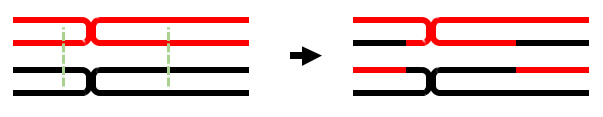
\includegraphics[width=0.7\textwidth]{../Figures/crossover2.jpg}%
	\vspace{-0.3cm}
	\captionof{figure}{Croisement en deux points.}\label{croisement2}%
\end{center}


\subsubsection{Opération de mutation}
La mutation apporte l'aléa nécessaire à une exploration efficace de l'espace des solutions en permettant de quitter les extrêmes locaux.
Il existe plusieurs façons de procéder à une mutation:


\paragraph{Inversement d'un gène}
Cette méthode consiste en l'inversement ou la troncature  d'un certain nombre fixe ou aléatoire de gènes d'une solution. La figure \ref{mut1} en est un exemple.
\begin{center}
	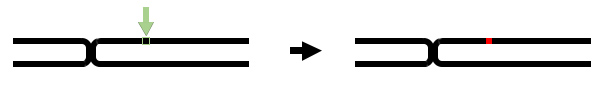
\includegraphics[width=0.7\textwidth]{../Figures/mutation1.jpg}%
	\vspace{-0.3cm}
	\captionof{figure}{Mutation avec inversement.}\label{mut1}%
\end{center}


\paragraph{Permutation de gènes}
Comme le montre la figure \ref{mut2}, 
la permutation de gènes nécessite d'abord la sélection de deux gènes sur l'individu (chromosome) à muter. Puis vient l'échange des deux valeurs (allèles) correspondantes, cela produit un nouvel individu. 
\begin{center}	
	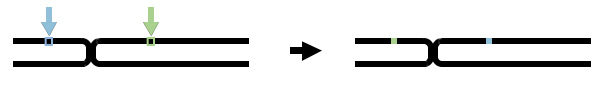
\includegraphics[width=0.7\textwidth]{../Figures/mutation2.jpg}%
	\vspace{-0.3cm}
	\captionof{figure}{Mutation avec permutation.}\label{mut2}%
\end{center}



\subsection{Pseudo code (GA incrémental)}
\begin{algorithm}[H]
	\TitleOfAlgo{GA}
	\vspace{-0.2cm}	
	\xdash[13.5cm]
	
	\SetAlgoLined
	\KwIn{$N$ : taille de la population, $MaxGen$ : nombre maximal de générations }
	\KwOut{meilleure solution}
	
	\SetKwFunction{GenerationSolutions}{GénérationSolutions}
	\SetKwFunction{Evaluation}{Evaluation}
	\SetKwFunction{MeilleurIndividus}{MeilleurIndividus}
	\SetKwFunction{PointCroisement}{PointCroisement}
	\SetKwFunction{Croisement}{Croisement}
	\SetKwFunction{NombreMutation}{NombreMutation}
	\SetKwFunction{Insertion}{Insertion}
	
	
	\Begin{
	$K \gets 0$\;
	$P_{k}\gets$ \GenerationSolutions(N)\;
	
	
	\Evaluation$(P_{k})$; \tcc{Évaluation de tous les individus de la population}
	
	\vspace{0.3cm}
	\While{$\neg$ $ BonneSolution$ \& $k < MaxGen$}{
		\tcc{Sélection des deux meilleurs parents de la population}
		$(Parent1 , Parent2)\gets$ \MeilleurIndividus$(P_{K})$\;
		
		\vspace{0.3cm}
		
		\tcc{Calcul da la position du point de croisement.}
		$i \gets$ \PointCroisement$(taille(solution))$\;
		\vspace{0.1cm}
		\tcc{Croisement des solutions parents}
		$Fils1 \gets$ \Croisement$(Parent1,Parent2,i)$\;
		$Fils2 \gets$ \Croisement$(Parent2,Parent1,i)$\;
		\vspace{0.1cm}
		\tcc{Évaluation des solutions fils}
		\Evaluation($Fils1$); 
		\Evaluation($Fils2$)\;
		
		\vspace{0.3cm}
		
		\tcc{Détermination du nombre de mutations.}
		$j \gets$ \NombreMutation$(taille(solution))$\;
		\vspace{0.1cm}
		\tcc{Mutation des solutions fils}
		$FilsMutant1 \gets Mutation(Fils1,j)$\;
		$FilsMutant2 \gets Mutation(Fils2,j)$\;
		\vspace{0.1cm}
		\tcc{Évaluation des solutions fils mutantes}
		\Evaluation($FilsMutant1$); \Evaluation($FilsMutant2$)\;
		
		
		\vspace{0.3cm}
		
		$K \gets K +1$\;
		\vspace{0.1cm}
		\tcc{Mise à jour de la population, suppression des solutions parents et insertion des solutions fils et fils mutantes.}
		$K \gets K +1$; 
		\Insertion$(P_{k},Newindividus)$\;	
	}
}
	
	\caption{Algorithme Génétique}
\end{algorithm}


\section{Conclusion}
Comme on a pu le constater, le comportement collectif des éléphants et des abeilles ainsi que la complexité de leur psychologie ont donné lieu à de puissants algorithmes de résolution orientés espaces des solutions. Ces derniers ont prouvé leur performance et leur efficacité face à de nombreux problèmes.
Ainsi, vu notre problématique, qui rappelons-le, consiste à détecter des cibles dans un espace complexe inconnu à l'aide de robots mobiles, nous avons choisi ces algorithmes intelligents pour la
résolution de notre problème compte tenu de leur robustesse. Le chapitre qui suit portera sur la modélisation de notre solution sur laquelle se baseront nos différentes approches mono-BSO, multi-BSO, EHO ainsi qu'ESWSA.



 
\let\cleardoublepage\clearpage
% Chapter 3

\chapter{Chapitre 3 : Modélisation du problème de recherche de cibles} % Main chapter title

\label{Chapter3} % For referencing the chapter elsewhere, use \ref{Chapter1} 
%----------------------------------------------------------------------------------------
\section{Introduction}
L'étape de modélisation d'un algorithme basé intelligence en essaim est centrale, elle requiert une bonne analyse faite au préalable, ce qui est particulièrement nécessaire lorsqu’il s'agit des problèmes complexes.

Ce chapitre est dédié à la description de notre modélisation et conception; celles-ci regroupent la représentation de l'espace de recherche, de la solution, de la fonction objectif ainsi que tous les autres composants de l'environnement de recherche. 
Par la suite, nous passerons en revue des travaux connexes relatifs aux stratégies d’évitement d’obstacles, avant d’enchaîner avec la strategie choisie avec justification de ce choix. Enfin nous nous pencherons sur le principe de fonctionnement de l'algorithme génétique, qui sera utilisé comme outil de réglage de paramètres des méta-heuristiques de recherche de cibles.


\section{Modélisation de l'environnement de recherche}
\label{vuEnv}
Nous avons modélisé notre environnement de recherche par une représentation 2D dite \textit{"grid based"}, sous forme d’une matrice comme le montre la figure \ref{env}. Notre environnement est caractérisé par une surface préalablement fixée, afin que les bordures délimitent la zone de recherche. La forme de l’environnement est carrée telle que :
\begin{equation}
Surface = Taille_{Cot\acute{e}} * Taille_{Cot\acute{e}}.
\end{equation}

Taille$_{cot\text{é}}$ : C'est la longueur d'un segment du carré.

Dans cette grille, chaque case contient une valeur ainsi qu'une position / coordonnée  \textit{(x,y)}, composée d'une abscisse (\textit{x}) et d'une  ordonnée (\textit{y}). Plusieurs valeurs sont admissibles dans les cases, celles-ci permettent de distinguer les objets comme suit : 
\begin{itemize}
	
	\item[$\bullet$] \textbf{Cible :} Dans ce cas la valeur assignée à cette position est égale à \textbf{1}.
	\item[$\bullet$] \textbf{Portée d'une cible :} La valeur est bornée par \textbf{0} et \textbf{1}, ces derniers exclus.
	
	(valeur(x,y) $\in$ \textbf{] 0,1 [} )
	
	\item[$\bullet$] \textbf{Obstacle :} Sa valeur est égale à \textbf{-1}.
	\item[$\bullet$] \textbf{Zone neutre :} Prend la valeur \textbf{0}.\\
\end{itemize}

\begin{center}	  
	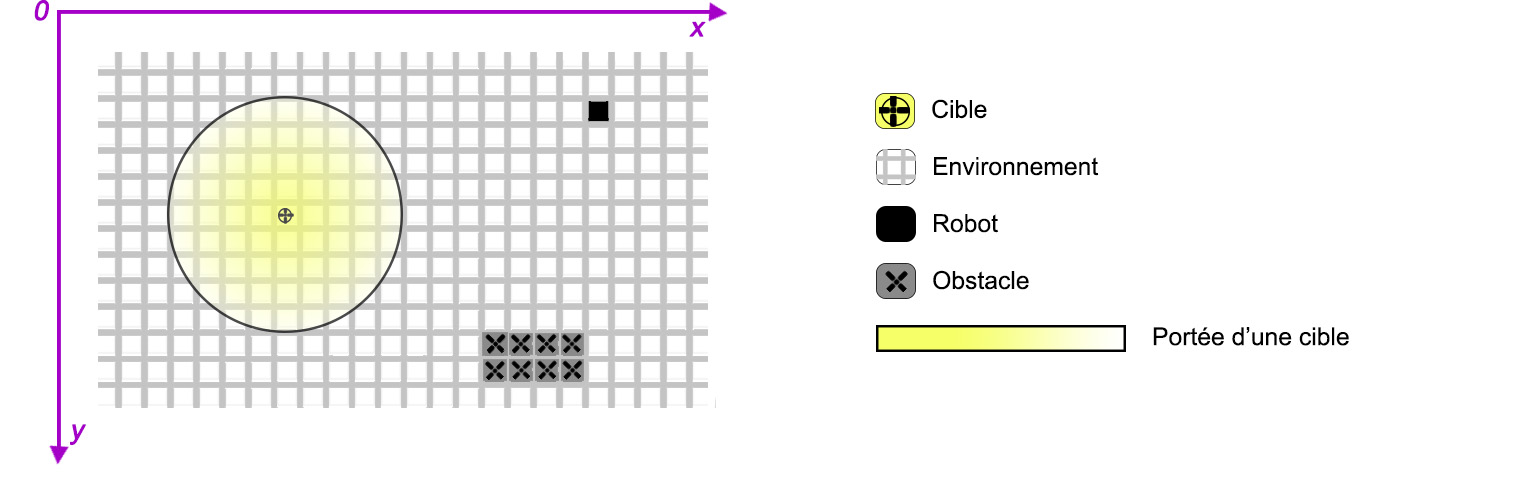
\includegraphics[width=1\textwidth]{env.jpg}%
	\vspace{-0.1 cm}
	\captionof{figure}{Représentation de l'environnement.}\label{env}%
\end{center}








\subsection{Représentation de la solution}
\label{sol}
Le but étant de trouver les cibles dans un environnement inconnu; l'espace des solutions à explorer n'est autre que notre environnement 2D composé de positions que nous appellerons aussi "solutions". 

Une solution optimale est une position géographique de coordonnée \textit{(x,y)}, elle est décrite par la valeur de sa case. La figure \ref{solution} représente une solution dans l'environnement de recherche. 

Dans le cas de multiples cibles on devra trouver autant de solutions optimales que de cibles, telles que chaque solution correspond à une case de valeur 1.
\begin{center}	  
	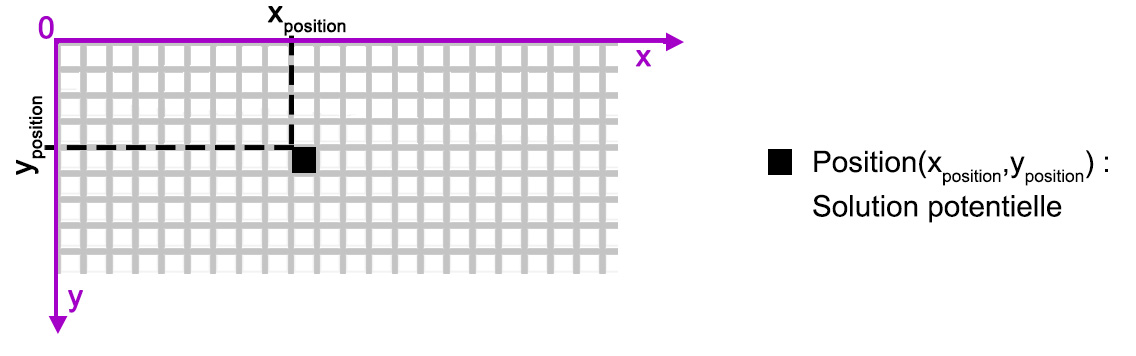
\includegraphics[width=0.8\textwidth]{Solution.jpg}%
	\vspace{-0.1 cm}
	\captionof{figure}{Représentation d'une solution dans notre modélisation.}\label{solution}%
\end{center}

Une solution doit satisfaire deux contraintes. D'abord, celle de la bornitude par les dimensions de l'environnement de recherche, ce dernier étant carré de taille $Taille_{Cot\acute{e}}$,
une solution est telle que:
\begin{equation}
\left\lbrace
\begin{array}{ccc}
0 \leq Position.x < Taille_{Cot\acute{e}}\\
0 \leq Position.y < Taille_{Cot\acute{e}}
\end{array}\right.
\end{equation}
Puis en tenant compte qu'une position contenant un obstacle n'est pas une solution admissible, soit :
\begin{equation}
environnement.get(Position.x , Position.y) \neq -1
\end{equation}



\subsection{Fonction objectif \label{fitness}}
Les solutions ont besoin d'être évaluées pour mesurer leurs distances par rapport à une cible. Ainsi, on pourra choisir la plus proche à chaque itération.

Notre fonction objectif varie selon l'intervalle borné suivant : [0,1]. Elle est égale à la valeur captée par les capteurs du robot, telle que plus la valeur se rapproche du 1, plus le robot est proche de la cible, car son émission est plus importante. Comme nous le verrons plus bas (Section \ref{porteee}), l'évaluation se fait sur les cases visibles par le robot, cela à travers son champ de vision (comportant un certain nombre de cases).

\subsection{Les cibles}
Une cible occupe une case unique ayant une valeur de 1, elle possède aussi une portée circulaire fixe, relative à l'émission de signaux perceptibles par les robots.\\ 

Comme on peut le voir dans la figure \ref{cible}, la portée décroît à partir de la position de la cible valant "1", jusqu'à la valeur "0" lorsque la distance par rapport à la cible excède la taille de la portée. Autrement dit, les valeurs représentatives des émissions de la cible sont inversement proportionnelles à la distance des positions incluses dans la portée.

\begin{center}	  
	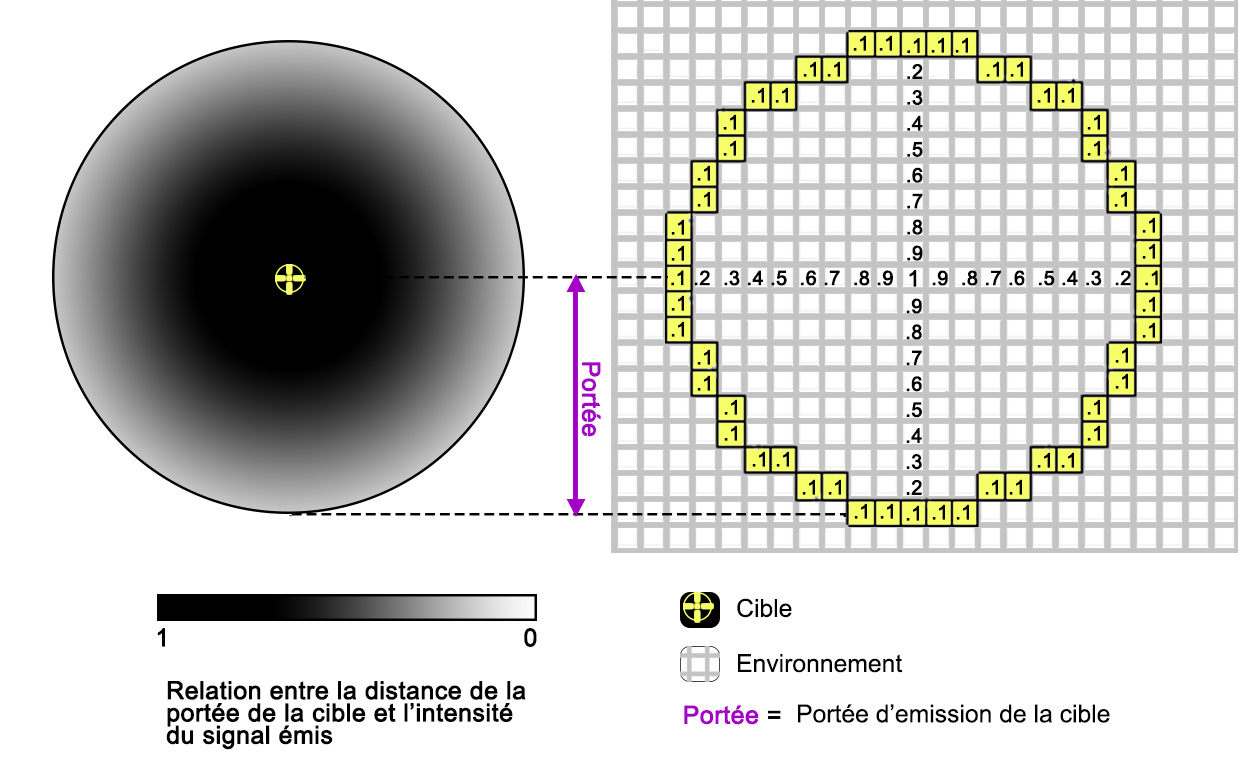
\includegraphics[width=0.8\textwidth]{cible.jpg}%
	\vspace{-0.1 cm}
	\captionof{figure}{Représentation de la portée d'une cible dans notre modélisation.}\label{cible}%
\end{center}

\paragraph{Remarque:}
Une fois qu'une cible est atteinte par un robot, elle est désactivée, elle arrête alors d'émettre des signaux. Nous avons modélisé cette action par la mise à zéro des cases de la matrice de l'environnement constituant la portée de cette cible.


\subsection{Les obstacles}
Un obstacle est considéré comme un objet fixe (statique) occupant une certaine surface de l'environnement et empêchant les robots de s'y positionner ou de la traverser.

Les environnements peuvent être catégorisés en trois (3) types selon la densité des obstacles, soient:

\begin{itemize}
	\item[$\bullet$] \textbf{Environnements simples (sans obstacles) :} Ceux-là ne contiennent que la ou les cible(s).
	\item[$\bullet$] \textbf{Environnements avec obstacles :} Comportant un nombre réduit d'obstacle de forme rectangulaire ainsi que la ou les cible(s).
	
	La taille d'un obstacle est comprise entre 2\% et 4\% de la taille de l'environnement. Quant au nombre d'obstacles, il appartient à l'intervalle [15 , 25] obstacles.
	
	\item[$\bullet$] \textbf{Environnements complexes :} Ils possèdent plus d'obstacles qui sont plus grands en termes de superficie que ceux de la catégorie précédente, en plus de la ou les cible(s).\\
	Dans ces environnements, la taille d'un obstacle est comprise entre 4\% et 6\% de la taille de l'environnement avec une densité de [25 , 35] obstacles.
\end{itemize}
\textbf{ }

Face aux différents types d'environnement existants, le choix d'une bonne stratégie d'évitement d'obstacles adaptée à notre modélisation devient crucial.


\section{Stratégies d'évitement d'obstacles}
Une stratégie d'évitement d'obstacles est nécessaire pour la navigation des robots dans des environnements à obstacles et complexes.
Le but des méthodes d'évitement d'obstacles est de trouver une trajectoire sûre (sans obstacles) entre deux positions, c’est-à-dire entre la position initiale d’un robot et sa position destination ou but.


\subsection{Description des approches existantes}
Les techniques les plus utilisées pour l'évitement d'obstacles sont décrites ci-dessous:

\subsubsection{Les algorithmes Bug  \cite{Sara,Bug}}
Les algorithmes Bug1 et Bug2 sont des méthodes anciennes et simples. Ils réduisent le robot en un point dans un plan 2D détectant les obstacles via capteurs tactiles. Ils sont basés sur deux comportements : \textit{"déplacement vers le but"} et \textit{"suivi d’une limite"}. 

\paragraph{Bug1 :}Tant que le robot n’a pas rencontré d’obstacle, il suit le comportement \textit{"déplacement vers le but"}, il se dirige tout droit vers la position but ($T$), lorsqu’il rencontre un obstacle en un point ($H_{i}$) il bascule vers le comportement \textit{"suivi d’une limite"} en faisant un tour complet sur l’obstacle. À partir de là il détermine le point du périmètre de l’obstacle  ($L_{i}$) le plus proche de la position but et s’y positionne. Ce processus se réitère jusqu’à atteindre la destination. (voir la figure \ref{bug}).

\paragraph{Bug2 :}
 Il exploite la première solution prometteuse qu’il trouve. Durant le comportement \textit{"déplacement vers le but"}, le robot se déplace selon des lignes droites reliant la position initiale ($S$) du robot et la position but ($T$). Quand un obstacle est rencontré, le robot adopte le comportement \textit{"suivi d’une limite"}, consistant à faire le tour de l’obstacle, jusqu’à atteindre un nouveau point  ($H_{i}$) qui appartient à la droite ($S$ , $T$) (voir la figure \ref{bug}).
Le processus est répété tant que la position but n’est pas atteinte par le robot.

\begin{center}	  
	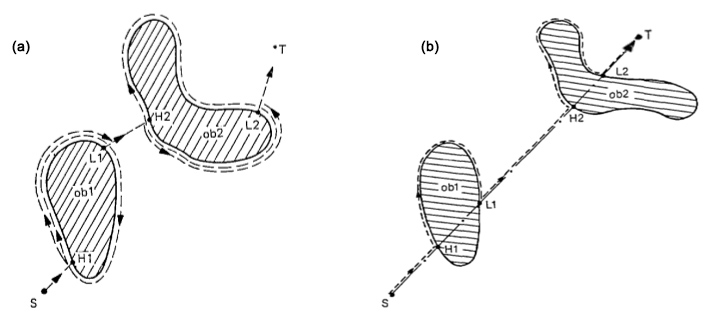
\includegraphics[width=0.75\textwidth]{../Figures/Bug.jpg}%
	\vspace{-0.1 cm}
	\captionof{figure}{Calcul du chemin du robot par les algorithmes Bug : (a) Bug1, (b) Bug2 \cite{Bug}. }\label{bug}%
\end{center}

\subsubsection{La méthode basée sur les champs de potentiel PF (Potential Field) \cite{Sara}}
Cette méthode a été proposée pour la première fois par Oussama Khatib \cite{Khatib}. Elle considère le robot comme une particule plongée dans un champ de potentiel, celui-ci régie par deux forces, soient : 

Force attractive $U_{attract}$: générée par le but.

Force répulsive $U_{r\acute{e}puls}$: générée par les obstacles.\\

Le robot calcule d’une manière itérative son prochain mouvement, suivant une direction résultante des sommes de différents champs potentiels (voir la figure \ref{pf}). La direction est donnée par la fonction :
 
\begin{equation}
F = - \bigtriangledown (U_{attract} + U_{r\acute{e}puls})
\end{equation}


\begin{center}	  
	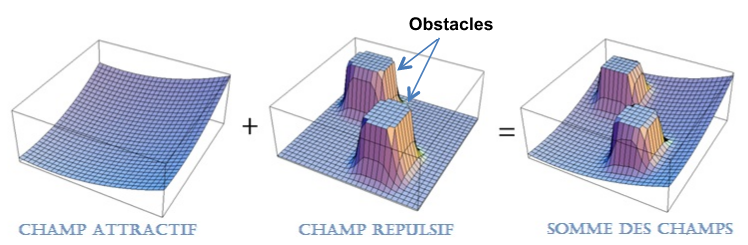
\includegraphics[width=0.75\textwidth]{../Figures/FP.png}%
	\vspace{-0.1 cm}
	\captionof{figure}{Champs de potentiel pour un environnement contenant deux obstacles et une position but.\cite{ImagePF}}\label{pf}%
\end{center}
	
\subsubsection{La méthode basée sur la fenêtre dynamique DW (Dynamic Window) \cite{Sara}}
La fenêtre dynamique est une méthode proposée par \textit{Burgardand} et \textit{Thruncite} \cite{window}. Elle vise à choisir un couple \textit{(v,w)} représentant respectivement la vitesse linéaire et angulaire du robot, permettant d’éviter les obstacles perçus localement. Sur la base des différents couples possibles, DW opte pour le couple de vitesses le plus pertinent. Comme le montre la figure \ref{dw}, la zone de recherche est limitée par une fenêtre dynamique basée sur les limitations dynamiques du robot et les vitesses admissibles et atteignables durant un laps de temps donné.
\begin{center}	  
	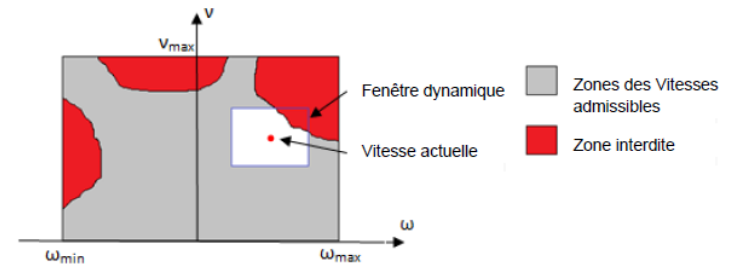
\includegraphics[width=0.75\textwidth]{../Figures/DW.png}%
	\vspace{-0.1 cm}
	\captionof{figure}{L'approche de la fenêtre dynamique montrant les régions admissibles et interdites par rapport à la fenêtre dynamique des vitesses atteignables par le robot \cite{Sara}.}\label{dw}%
\end{center}
		
\subsubsection{La logique floue}
La logique floue est une branche de l’intelligence artificielle et des mathématiques qui a été appliquée à des problèmes de commandes (Bühler 1997) \cite{FuzzyLogic}. Cette technique se base sur la déduction de deux commandes : la vitesse linéaire et angulaire selon les variables floues des données en entrées, qui sont : la vitesse (\textit{v}) du robot et l’angle ($\alpha$) entre le robot et l’obstacle, en plus d’une base de règles afin d’éviter les obstacles \cite{Cai2013}.
		
		
\subsubsection{L'échantillonnage de l'espace d'entrée ISS (Input Space Sample) }
À partir d'un état initial du robot, le modèle prédictif du système est utilisé pour la génération d'un ensemble de trajectoires. Celles-ci peuvent être triées selon une fonction de coût. L'exemple d'un ensemble de trajectoires générées en utilisant la technique par échantillonnage de l'espace d'entrées est illustré dans la figure \ref{ech}.

Selon les obstacles visibles par le robot, certaines trajectoires seront bannies de l'ensemble des trajectoires admissibles \cite{Sara}, comme il est le cas de \textit{S1, S2, S7, S8} et \textit{S9}.
		
Les travaux de \textit{Kelly} et \textit{Stentz} \cite{echantillonnage} font partie des premiers travaux basés sur cette technique.
		
\begin{center}	  
	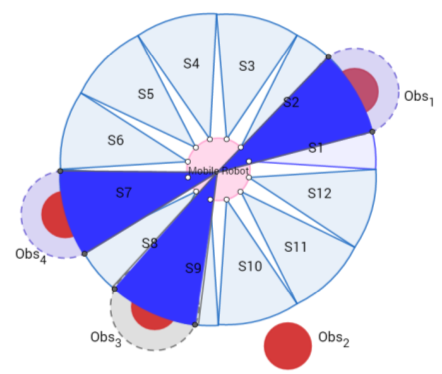
\includegraphics[width=0.5\textwidth]{../Figures/echan.png}%
	\vspace{-0.1 cm}
	\captionof{figure}{Ensemble de trajectoires
	générées par échantillonnage de l'espace d'entrées \cite{imageEch}.}\label{ech}%
\end{center}


\subsection{Discussion et choix}
Les algorithmes bug1 et bug2 sont faciles à mettre en œuvre et peu gourmands en termes de  mémoires. Cependant, ils nécessitent des déplacements supplémentaires et souvent la trajectoire trouvée est loin d'être optimale (trajectoires comportant trop de détours supplémentaires augmentant ainsi la distance pour atteindre la position but).\\ 

Les méthodes de champ de potentiel et de logique floue, sont facilement adaptables aux formules des méta-heuristiques disposant d’une vélocité telles qu'ESWSA. En revanche, elles sont difficiles à mettre en pratique pour d'autres méthodes dont BSO et EHO, car le calcul des positions est indépendant de la direction de l’ancienne position vers la nouvelle.

De plus, elles ne permettent pas de détecter un passage entre des obstacles assez proches. Encore pire, le robot risque de ne jamais atteindre la position but, si ce dernier est à proximité directe d'un obstacle.\\  

D'autre part, la méthode de la fenêtre dynamique (DW) n'est pas sujette aux limites précédemment citées. Mais elle peut être vu comme une recherche exhaustive d'une trajectoire optimale selon la dimension de la fenêtre, car pour une fenêtre de taille (\textit{x, y}) nous aurons \textit{x * y} paires (\textit{v, w}) à tester.\\

Enfin, la stratégie d'échantillonnage, n'est pas concernée par les problèmes cités ci-dessus dans le cadre de notre modélisation. Elle est simple et efficace, mais son plus grand avantage est qu'elle peut être directement adaptée ou intégrée dans d'autres concepts ou algorithmes.\\

Suite à l'analyse faite ci-dessous des avantages et inconvénients de chaque approche par rapport à notre modélisation, notre choix s'est porté sur la stratégie d'\textbf{échantillonnage} qu'on a jugé comme étant la plus adéquate.


\subsection{Paramètres de la méthode d'échantillonnage}
L'échantillonnage de l'espace local des robots est régi par plusieurs paramètres devant être fixés au préalable, soient : 

\subsubsection{Champ de vision}
L'espace local d'un robot est divisé en quatre zones de 90$\textordmasculine$, comme le montre la figure \ref{zones} : $"$NE: Nord-Est, NW: Nord-Ouest, SW: Sud-Ouest, SE: Sud-Est$"$.

Le champ de vision d'un robot est d'un angle de 90$\textordmasculine$, choisi selon la zone contenant la droite reliant la position du robot à la position but.\\

Afin de déterminer la zone concernée, nous devons effectuer deux opérations de soustraction sur les coordonnées du robot ($x_{R}$,$y_{R}$) et celles de la position destination ($x_{but}$,$y_{but}$).
Les zones relatives aux résultats de ces opérations sont représentées dans le schéma ci-dessous. 
\begin{center}	  
	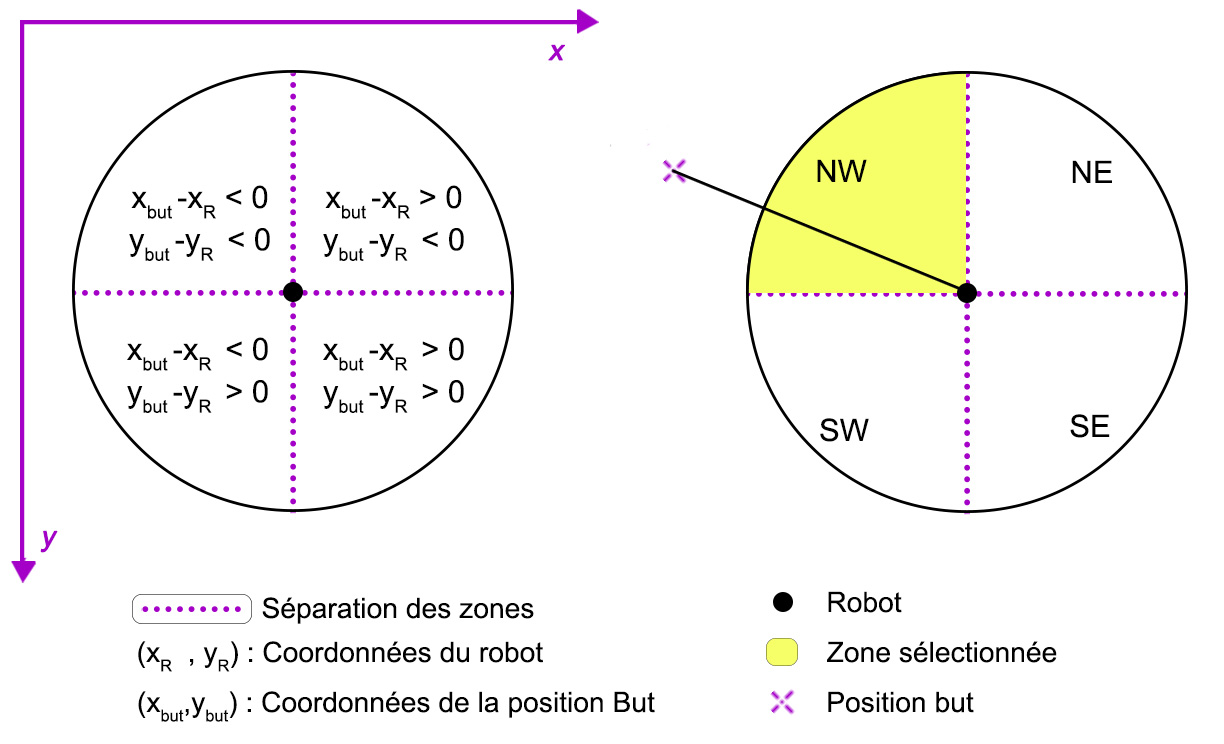
\includegraphics[width=0.7\textwidth]{Angle_de_vue.jpg}%
	\vspace{-0.1 cm}
	\captionof{figure}{Détermination de l'angle de vue d'un robot dans notre modélisation.}\label{zones}%
\end{center}

\subsubsection{Portée locale d'un robot}
\label{porteee}
Chaque robot possède une portée locale, celle-ci forme une surface circulaire dont le robot est le centre. Le rayon de ce cercle est limité par la portée des capteurs présents sur le robot.

Dans notre modélisation, cette portée locale est fixée à une distance de dix positions du robot. La zone maximale visible par chacun de nos robots est représentée dans la figure \ref{portee} qui suit:


\begin{center}	  
	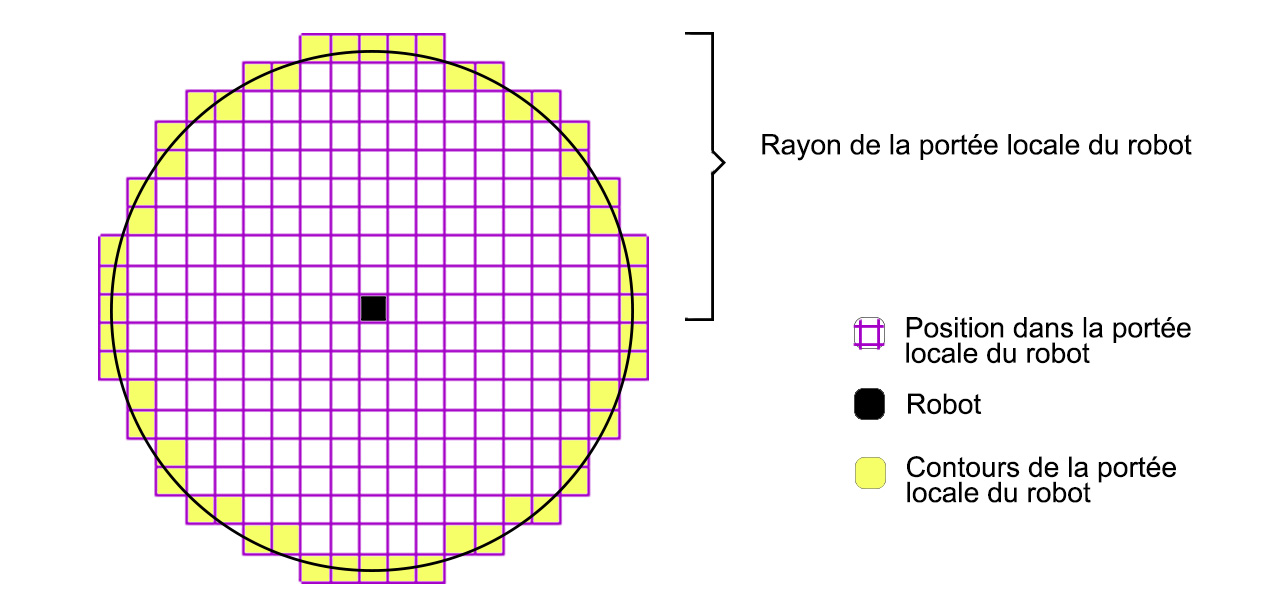
\includegraphics[width=0.69\textwidth]{portee.jpg}%
	\vspace{-0.1 cm}
	\captionof{figure}{Représentation de la portée locale d'un robot dans notre modélisation.}\label{portee}%
\end{center}

Il est à noter que les robots ont cette portée de vue durant tout le parcours fait, c'est-à-dire que tout le long de leurs déplacements, une vérification de cette surface accessible est effectuée. 

Nos robots prennent place dans les meilleures positions visibles dans leurs portées, cela à travers le processus suivant :\\

\begin{algorithm}[H]
	\SetAlgoLined
	\KwIn{$P$ : position du robot,\\
		\hspace{1.3cm}$portee$ : Portée des capteurs = 10,\\
		\hspace{1.3cm}$env$ : Matrice de dimension M*M}
	
	\KwResult{meilleurePosition : Meilleure position maximisant la fonction objectif}
	
	\vspace{0.2cm}
	
	%\tcc{Initialisation}
	$meilleureLocale \gets env.valeur( P_x , P_y)$\;
	$meilleurePosition \gets Position(P_x,P_y)$\;
	
	\vspace{0.2cm}
	
	%	\tcc{Evaluation}
	\For{i $\gets$ -portee \KwTo +portee}{
		\For{j $\gets$ -portee \KwTo +portee}
		{  
			\vspace{0.2cm}
			
			%\tcc{Vérification si la position est valide (bornée par les dimensions de l'environnement) et est dans le rayon accessible}
			
			\If{$env.valide( P_x + i, P_y + j ) $ \textbf{And}  $ i^2 + j^2 \leq portee^2$} {
				$b \gets env.valeur (  P_x + i, P_y + j)$\;
				\If{$meilleureLocale < b$ }{
					$	meilleureLocale \gets b $\;
					$meilleurePosition \gets Position( P_x + i, P_y + j)$\;
				}
			}
		}
	}
	
	\Return$meilleurePosition$\;
	
	\caption{Meilleure position dans la portée du robot}
\end{algorithm}



\subsubsection{Trajectoire}
Une trajectoire est modélisée par une droite reliant deux positions successives, cette droite est un ensemble de cases extraites selon l'équation de la droite, \textit{Bresenham} \cite{line} l'a exploité pour en déduire l'algorithme \ref{codeLine} suivant : 




\noindent
\begin{minipage}[t]{0.45\textwidth}
	\vspace{-0.5cm}
	\begin{algorithm}[H]
		
		\SetAlgoLined
		\DontPrintSemicolon
		\KwIn{$x_0$,$y_0$,$x_1$,$y_1$ }
		%\KwOut{}
		
		\SetKwData{dx}{dx}
		\SetKwData{dy}{dy}
		\SetKwData{sx}{sx}
		\SetKwData{sy}{sy}
		\SetKwData{x}{$x_{0}$}
		\SetKwData{y}{$y_0$}
		\SetKwData{xx}{$x_{1}$}
		\SetKwData{yy}{$y_1$}
		\SetKwData{err}{err}
		\SetKwData{e}{e2}
		
		\SetKwFunction{Abs}{Abs}
		\SetKwFunction{setPoint}{setPoint}
		
		\dx = \Abs(\xx-\x);
		\dy = -\Abs(\yy-\y);
		
		\lIf{\x<\xx}{\sx = 1;}\lElse{\sx = -1;}
		\lIf{\y<\yy}{\sy = 1;}\lElse{\sy = -1;}
		
		\err = \dx+\dy;
		
		\While{True}{
			\setPoint(\x,\y);
			
			\e = 2*\err;
			
			\lIf{\e >= \dy} {
				\lIf{\x == \xx}{ break;}
				\err += \dy; \x += \sx;
			}
			\lIf{\e >= \dx} {
				\lIf{\y == \yy}{ break;}
				\err += \dx; \y += \sy;
			}
		}
		\caption{line-drawing algorithm \cite{line}}
		\label{codeLine}
	\end{algorithm}
\end{minipage}\hfill
\begin{minipage}[t]{0.45\textwidth}
	%\vspace{0.1cm}
	\centering\raisebox{\dimexpr \topskip-\height}{%
		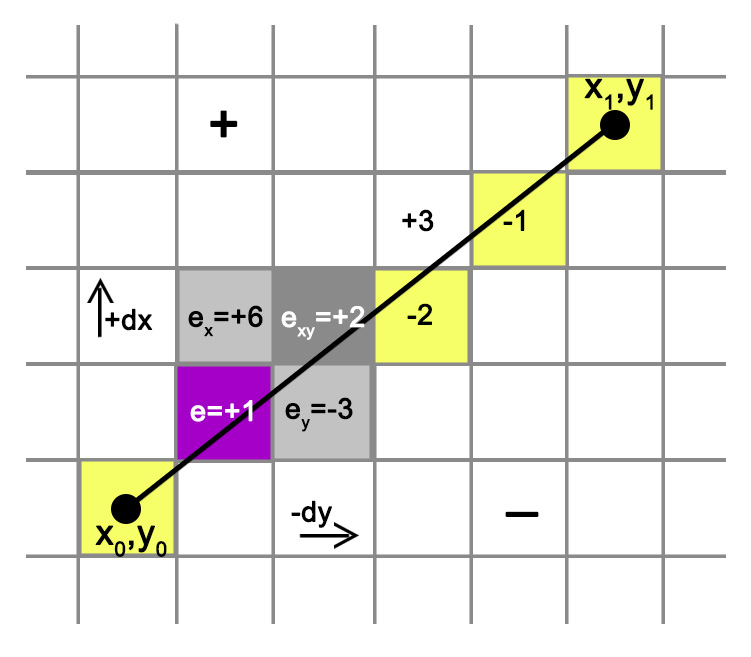
\includegraphics[width=1\textwidth]{line.jpg}}
	\captionsetup{width=0.7\linewidth}
	\captionof{figure}{Sélection des points (cases) d'une droite avec l'algorithme de BRESENHAM.}
	\label{line}
\end{minipage}

\vspace{0.5cm}
Grâce à cet algorithme de Bresenham, nous pouvons au lieu de chercher à dessiner la droite à partir de deux positions, comme le montre la figure \ref{line}, l'exploiter pour vérifier si une trajectoire comporte des obstacles ou non.




\subsubsection{Critères de choix de la trajectoire}
Une fois que nous sommes en mesure de déterminer si une trajectoire est admissible (sans obstacles) ou interdite (contient des obstacles), vient l'étape de sélection de la trajectoire admissible la plus adéquate.

Cette seconde étape revient à choisir la meilleure trajectoire parmi celles admissibles, en minimisant la distance entre la position choisie (accessible) et la position destination de notre robot.
Les deux étapes sont illustrées dans la figure \ref{choix} ci-dessous :

\begin{center}	  
	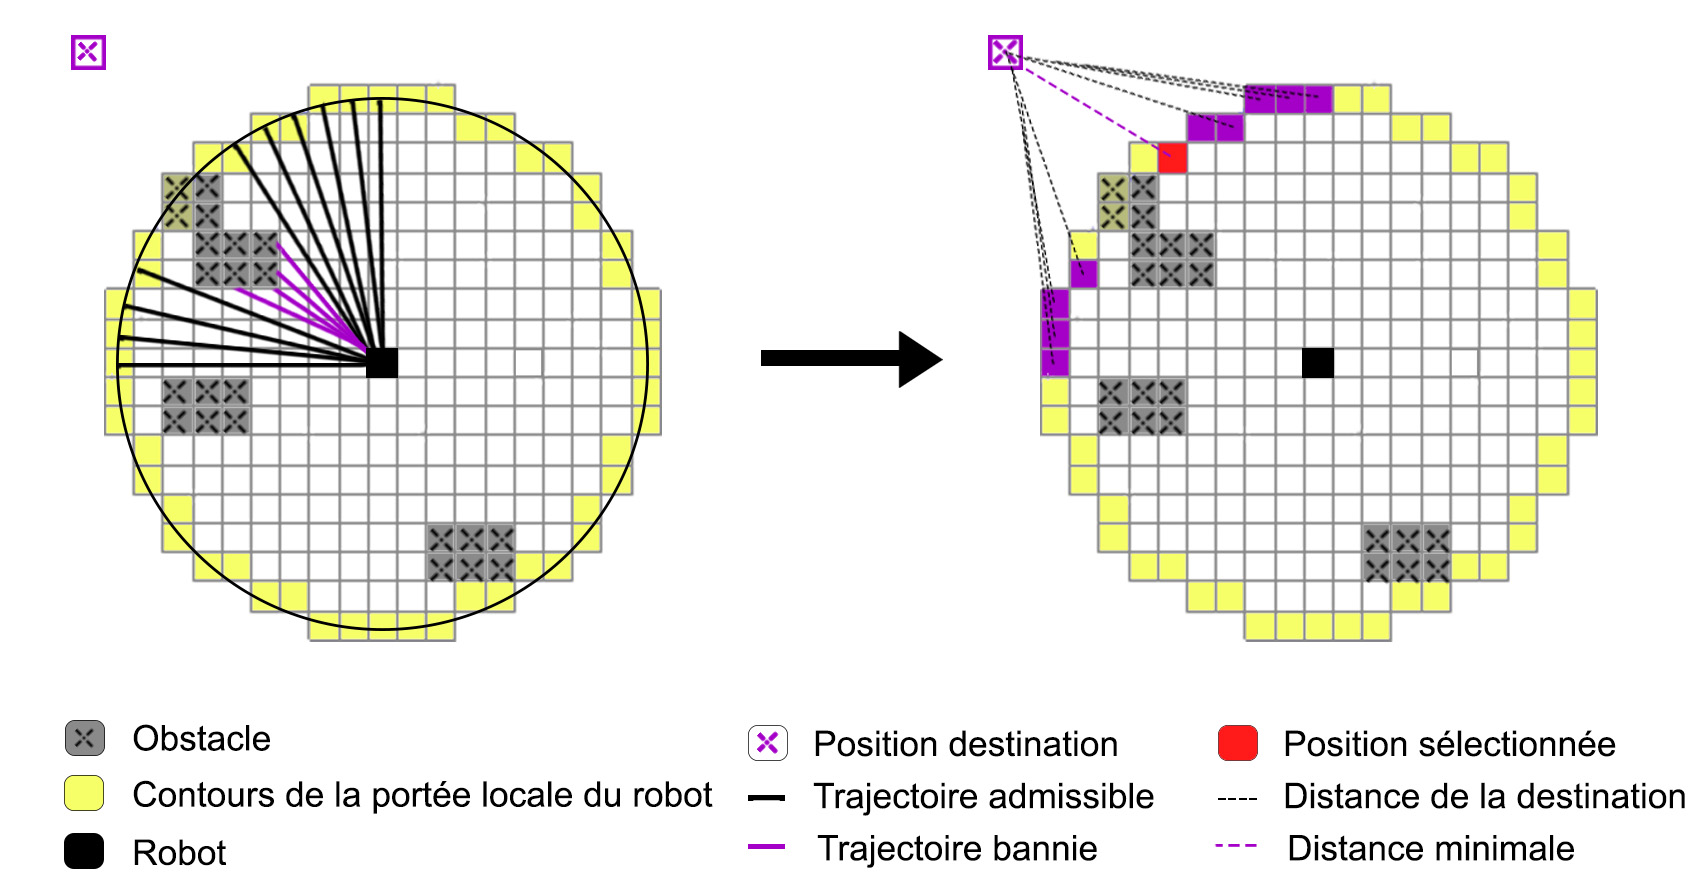
\includegraphics[width=0.9\textwidth]{choix.jpg}%
	\vspace{-0.1 cm}
	\captionof{figure}{Choix de la trajectoire à suivre par le robot dans un environnement à obstacle.}\label{choix}%
\end{center}

\paragraph{Remarque:} Si la position de destination est à une distance inférieure à la portée du robot (inférieure à dix cases.), le même procédé est effectué avec une portée égale à la distance entre le robot et la position destination.

\paragraph{Autres cas de figure}

Plusieurs cas de figure existent selon la position des obstacles par rapport à celle du robot, pour cela nous avons étudié toutes les possibilités pour garantir le bon fonctionnement de notre approche dans tous les environnements.\\

La figure \ref{choix_annexe} représente deux cas de figure se produisant souvent dans des environnements complexes.
Lorsque aucune trajectoire admissible n'est trouvée dans le champ de vision initial du robot (90$\textordmasculine$), on l'élargit aux zones adjacentes de 90$\textordmasculine$ allant ainsi à un champ de vision qui équivaut à 270 $\textordmasculine$. Ceci simulera une rotation du robot sur lui-même (voir schéma de droite).

Si le robot ne trouve toujours pas de trajectoire admissible, une nouvelle position destination est demandée.\\

Dans le cas où la position destination est alignée sur un des deux axes avec la position actuelle du robot (c'est-à-dire qu'ils possèdent la même abscisse ou même ordonnée), notre robot aura une vue sur les 180$\textordmasculine$ dont la droite (position du robot - position destination) est commune (schéma de gauche).
\noindent
\begin{center}	  
	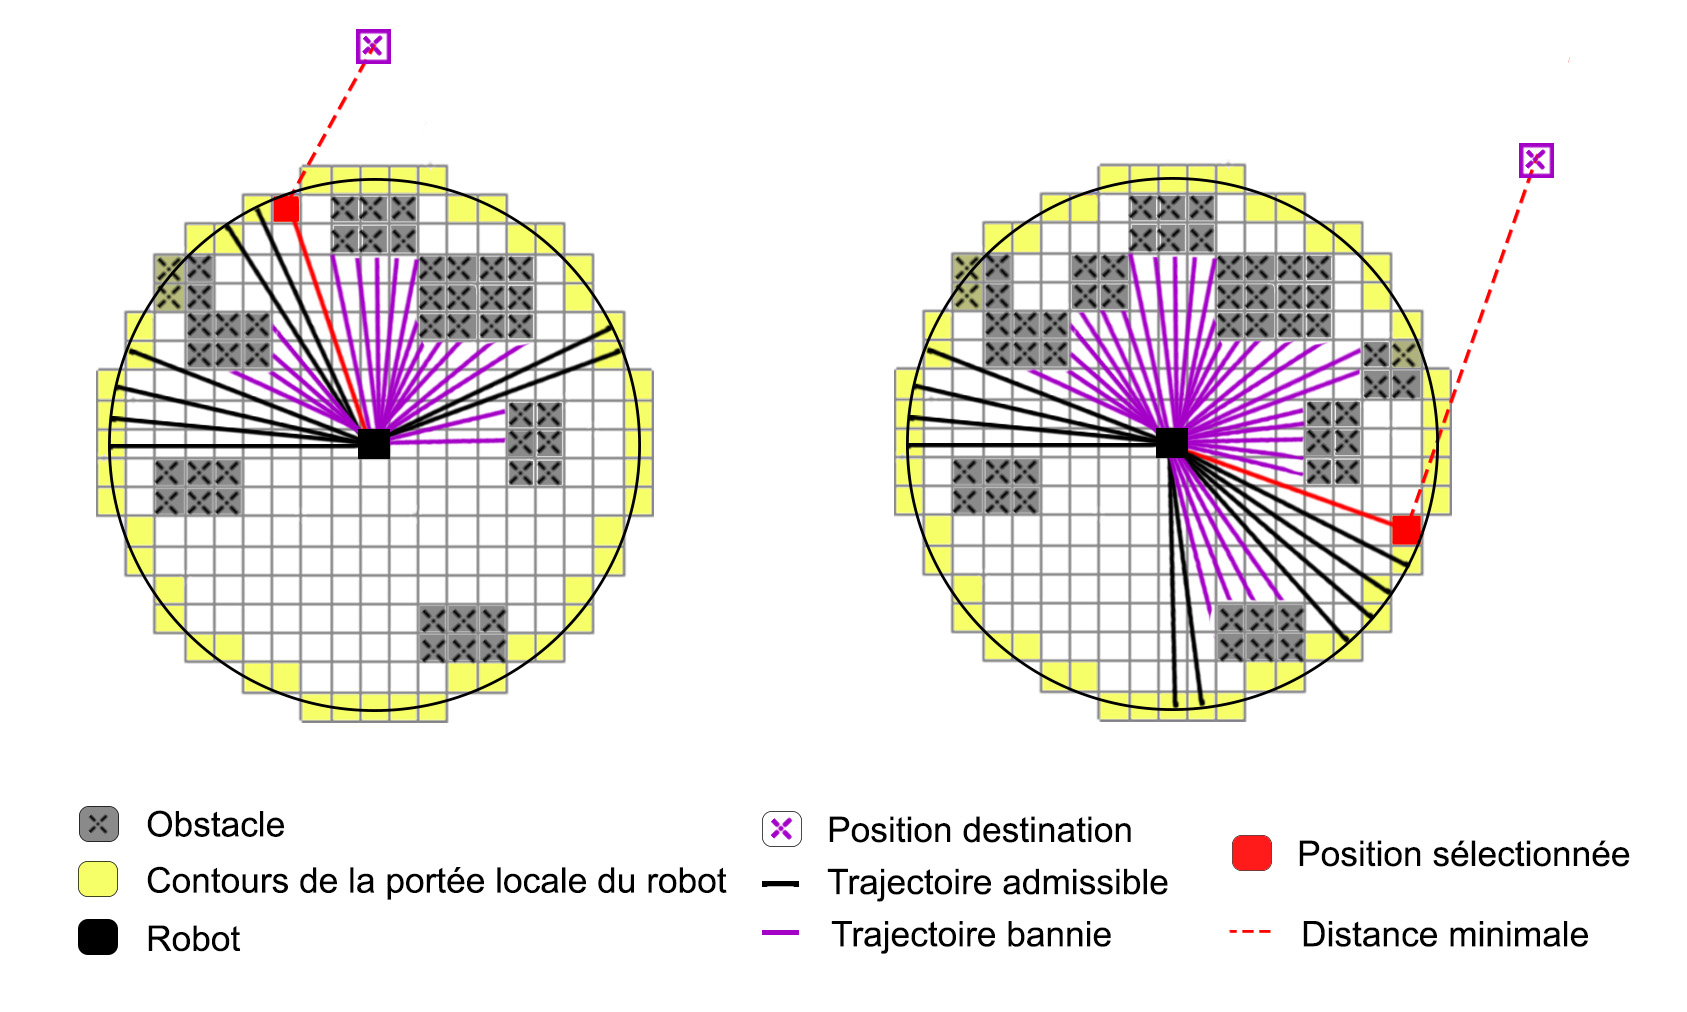
\includegraphics[width=0.9\textwidth]{choix_annexe.jpg}%
	\vspace{-0.1 cm}
	\captionof{figure}{Choix de la trajectoire à suivre par le robot dans des situations complexes.}\label{choix_annexe}%
\end{center}


\section{Auto-Paramétrage avec GA}
\label{génétique}
\subsection{Modélisation}
\subsubsection{Solution}
Une solution pour notre algorithme génétique est un paramétrage pour une de nos approches de résolution. Elle est représentée par un vecteur de paramètres.\\
Vu que nos méta-heuristiques n'ont ni le même nombre de paramètres, ni les mêmes plages de valeurs de ces paramètres, la taille de la solution ainsi que les contraintes singulières relatives à chaque approche seront fixées, celles-ci sont représentées dans le tableau \ref{ContrGA} ci-dessous :

\begin{table}[h]
	\centering
	\begin{tabular}{lllllllllllllllll} 
		%\toprule
		\textbf{Paramètres} &  \textbf{Paramètre 1} &
		\textbf{Paramètre 2} & \textbf{Paramètre 3} & \textbf{Paramètre 4}\\ 
		\hline
		\textbf{BSO} & Flip & nbrBees & MaxChance &  -\\ 
		\hline
		\textbf{Min} & 1 & 1 & 1 &  -  \\ 
		\hline
		\textbf{Max} & 100 & 25 & 4 &  - \\
		\hline
		\hline
		\textbf{Multi-BSO} & Flip & nbrBees & MaxChance &  nbSwarm\\ 
		\hline
		\textbf{Min} & 1 & 1 & 1 & 1  \\ 
		\hline
		\textbf{Max} & 100 & 5 & 4 & 5 \\
		\hline
		\hline
		\textbf{EHO} & nbrClan & nbrElephant & Alpha &  Beta\\ 
		\hline
		\textbf{Min} & 1 & 1 & 0.1 & 0.1  \\ 
		\hline
		\textbf{Max} & 5 & 5 & 0.9 & 0.9 \\
		\hline
		\hline
		\textbf{ESWSA} & nbElephant & P & inertia Weight &   - \\ 
		\hline
		\textbf{Min} & 1 & 0.1 & 0.1 & -  \\ 
		\hline
		\textbf{Max} & 25 & 0.9 & 0.9 & - \\
		\hline
		%\bottomrule
	\end{tabular}
	\captionsetup{width=1\linewidth}
	\caption{Contraintes sur les paramètres des méta-heuristiques.}
	\label{ContrGA}
\end{table}






\subsubsection{Espace des solutions}
L’espace des solutions diffère selon l'approche à paramétrer. Pour une approche donnée, Il s'agit de l’ensemble des combinaisons possibles des différentes valeurs de chaque paramètre de cette approche.\\
Comme présenté dans le tableau \ref{ContrGA}, les domaines de chaque paramètre sont clairement définis, ainsi l'espace des solutions de notre algorithme génétique comporte:

\begin{itemize}
	\item[$\bullet$] Pour BSO : 100 $\times$ 25 $\times$ 4 = 10 000 solutions.
	\item[$\bullet$] Pour Multi-BSO : 100 $\times$ 5 $\times$ 4 $\times$ 5 = 10 000 solutions.
	\item[$\bullet$] Pour EHO : 5 $\times$ 5 $\times$ 9 $\times$ 9 = 2 025 solutions.
	\item[$\bullet$] Pour ESWSA : 25 $\times$ 9 $\times$ 9 = 2 025 solutions.
\end{itemize}

\subsubsection{Fonction objectif}
Rappelons que l’objectif de notre algorithme génétique est de trouver la meilleure combinaison de paramètres pour nos approches de recherche de cibles. C’est pourquoi notre évaluation se résume en une exécution d’une approche de recherche. Compte à notre fonction objectif, elle se décompose en deux sous fonctions objectif:
\begin{enumerate}
	\item Meilleure en termes de nombre de cibles trouvées, qui est à maximiser.
	\item Meilleure en termes de nombre d'itérations, celle-ci est à minimiser.
\end{enumerate}

Ces deux fonctions suivent une hiérarchie conforme à l’ordre dans lequel nous les avons citées. La meilleure solution est celle qui permet de trouver le maximum de cibles d’abord, mais aussi qui minimise le nombre d’itérations effectué pour les atteindre.

\subsubsection{Population}
La taille de la population \textbf{N} initiale est un paramètre à régler par expérimentations, il dépend aussi de l'espace des solutions à explorer.

\subsubsection{Croisement}
Un seul point de croisement est choisi, il est défini de manière aléatoire selon la contrainte suivante:
\begin{equation}
0 < \textbf{pointCroisement} < nbrParamètres
\label{crois}
\end{equation}
Une fois le point de croisement déterminé, nous passons à la formation des solutions fils, grâce à l'opérateur de concaténation.
%telles que:
%\begin{equation}
%\label{eq:fils1}
%S1_{fils} = Concat
%\left\lbrace
%\begin{array}{ccc}
%Premier \Longrightarrow pointCroisement - 1  & \text{éléments de S1}\\
%pointCroisement \Longrightarrow Derniers  & \text{éléments de S2}
%\end{array}\right.	 
%\end{equation}
%
%\begin{equation}
%\label{eq:fils2}
%S2_{fils} = Concat
%\left\lbrace
%\begin{array}{ccc}
%Premier \Longrightarrow pointCroisement - 1  & \text{éléments de S2}\\
%pointCroisement \Longrightarrow Derniers  & \text{éléments de S1}
%\end{array}\right.	 
%\end{equation}
La figure \ref{gacroisement} suivante explicite le déroulement d'un croisement.
\begin{center}	  
	\captionsetup{width=1\linewidth}
	
\includegraphics[width=0.9\textwidth]{crossGA.jpg}%
	\vspace{-0.1 cm}
	\captionof{figure}{Croisement de deux solutions.}\label{gacroisement}%
\end{center}


\subsubsection{Mutation}
Une mutation est le remplacement d'un ou plusieurs paramètres de notre solution par une valeur aléatoire, toujours en respectant les contraintes d'intervalle de chaque paramètre cité dans le tableau \ref{ContrGA}. On choisit de faire une seule mutation aléatoire explicitée dans la figure \ref{gamutation} suivante:
\begin{center}	  
	\captionsetup{width=1\linewidth}
	
\includegraphics[width=0.9\textwidth]{mutGA.jpg}%
	\vspace{-0.1 cm}
	\captionof{figure}{Mutation d'une solution.}\label{gamutation}%
\end{center}



\subsection{Fonctionnement}
La méta-heuristique GA comporte une population de \textbf{N} individus dont nous essayons d'améliorer les gènes pour obtenir le meilleur individu au fil des générations.
L'organigramme de la figure \ref{ga} décrit ce processus en détail.\\

Tout d'abord, les bornes (inférieurs et supérieurs) de chaque paramètre, pour chaque approche doivent être initialisées, afin que les valeurs générées pour chaque individu soient cohérentes avec l'espace des solutions.
Puis, les \textbf{N} individus de notre population seront générés et évalués un à un selon la fonction objectif décrite plus haut, avant leur insertion dans la population \textbf{P}.
L'auto-paramétrage suit les étapes suivantes :

\subsubsection{Sélection des deux meilleures solutions}
Les deux meilleures solutions de la population \textbf{P} de la  génération \textit{"t$^{i\grave{e}me}$"} sont sélectionnées, soient \textit{"S1"} et \textit{"S2"}.

Ces deux parents sont supprimés de la population après sélection.

\subsubsection{Croisement des deux solutions (parents)}
On effectue lors de cette phase un croisement sur \textit{"S1"} et \textit{"S2"} selon le point de croisement \textbf{pointCroisement}, produisant ainsi deux autres solutions enfants: \textit{"S1$_{fils}$"} et \textit{"S2$_{fils}$"}. 

\subsubsection{Évaluation des solutions fils}
On évalue ensuite les solutions enfants \textit{"S1$_{fils}$"} et \textit{"S2$_{fils}$"} selon la fonction objectif (nombre de cibles trouvées et nombre d'itérations).

\subsubsection{Mutation des solutions fils} 
Les solutions fils subiront un nombre \textbf{nbrMutation} de mutations. Il en résultera deux autres solutions mutantes, qu'on notera : \textit{"S1'$_{fils}$"} et \textit{"S2'$_{fils}$"}. 

\subsubsection{Évaluation des solutions mutantes}
Comme pour les solutions fils, les solutions mutantes seront évaluées selon la fonction objectif.

\subsubsection{Injection des solutions résultantes dans la population}
Une fois les quartes solutions évaluées à savoir : \textit{"S1$_{fils}$"}, \textit{"S2$_{fils}$"}, \textit{"S1'$_{fils}$"} et \textit{"S2'$_{fils}$"}, on les insère dans la population courante.

\subsubsection{Passage à la génération suivante}
Après avoir enrichie la population avec les nouveaux individus, on incrémente  l'indice de génération \textit{"t"}, afin de passer à la génération suivante.

\subsubsection{Critère d'arrêt}
Toutes ces étapes du processus de paramétrage par l'algorithme génétique, seront réitérées jusqu'à ce que le nombre de générations \textbf{MaxGen} soit atteint. 



Pour notre solution finale, nous sélectionnons les cinq meilleures solutions de la population, pour en calculer la moyenne.


\noindent
\begin{center}	  
	\captionsetup{width=1\linewidth}
	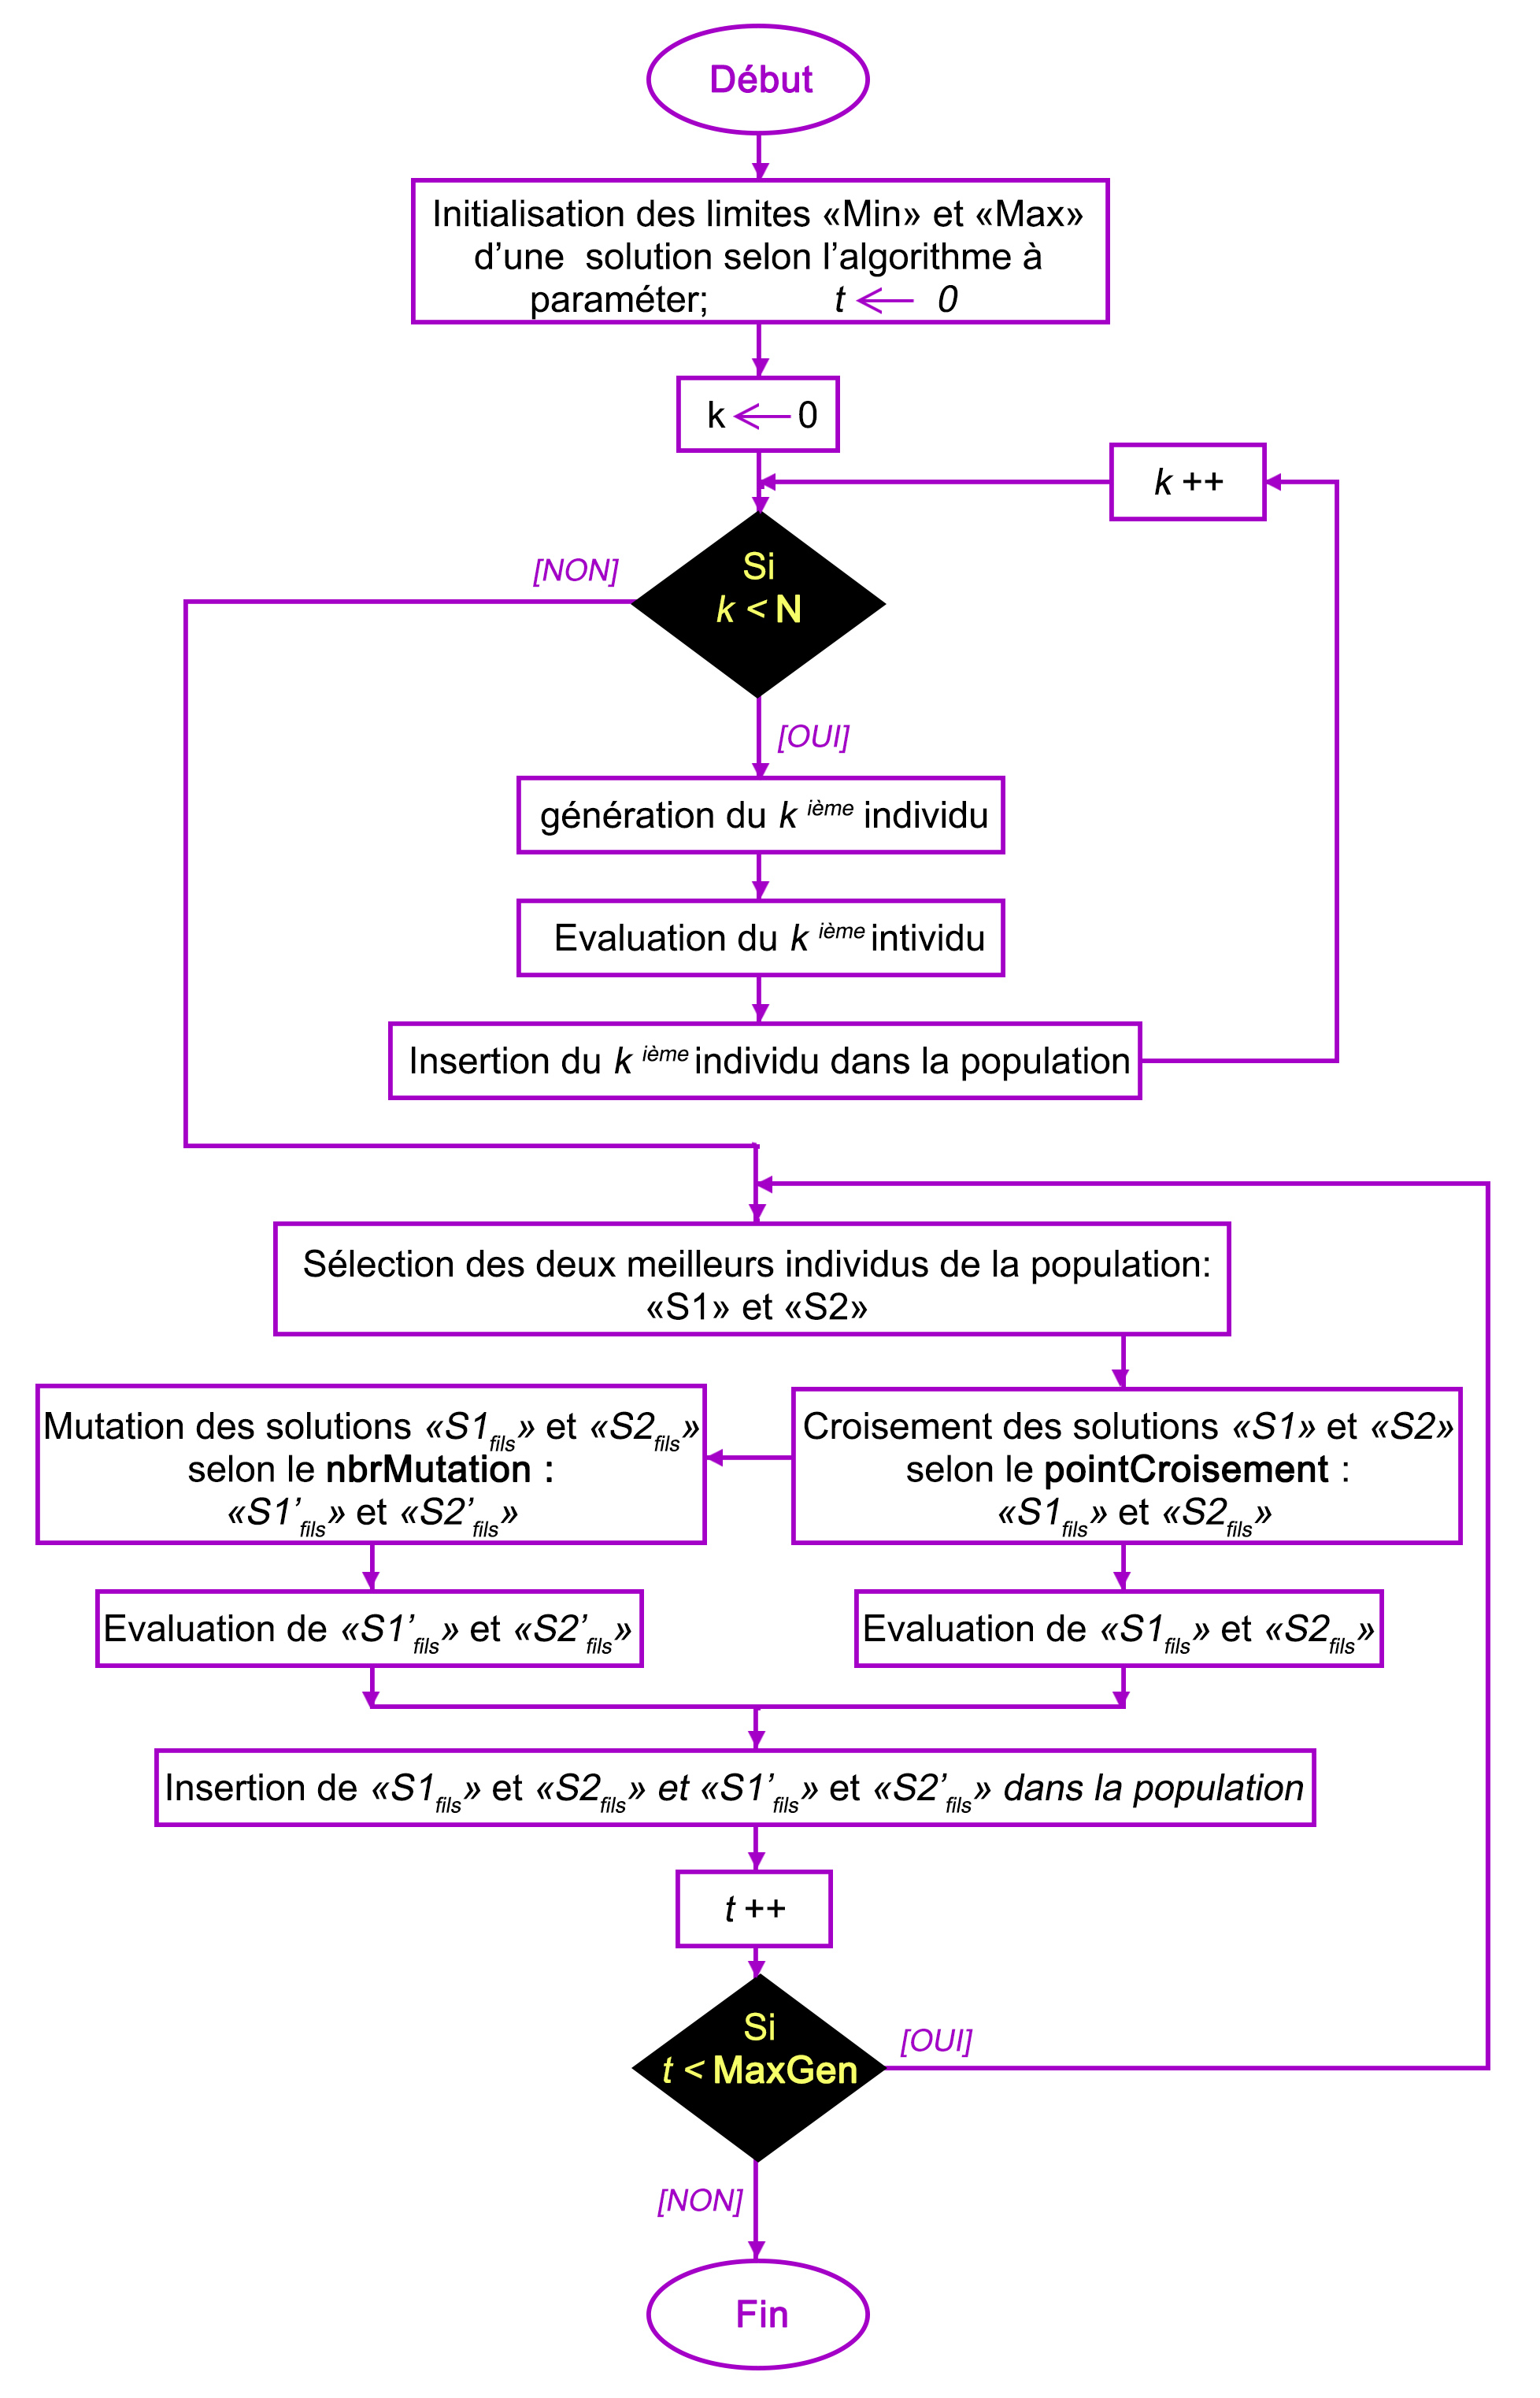
\includegraphics[width=0.79\textwidth]{ga.jpg}%
	\vspace{-0.3 cm}
	\captionof{figure}{Organigramme du mode de fonctionnement de la méthode GA.}\label{ga}%
\end{center}


\section{Conclusion}
Ce chapitre a fait l'objet de la modélisation de tous les aspects de notre problème, c'est à partir de cette modélisation que nous avons choisie une stratégie d'évitement d'obstacles applicable à toutes nos méthodes de résolution basées essaims. Tous les détails relatifs à son fonctionnement y sont présentés. Enfin, nous avons explicité l'usage de l'algorithme Génétique pour le paramétrage automatique.
Ces parties communes à l'ensemble de nos approches de recherche de cibles définies, nous nous attelons à présenter nos approches de recherche de cibles, commençant par BSO dont il est question dans le chapitre suivant.



% Chapter 3

\chapter{Chapitre 4 : BSO pour le problème de recherche de cibles} % Main chapter title

\label{Chapter4} % For referencing the chapter elsewhere, use \ref{Chapter1} 
%----------------------------------------------------------------------------------------
\section{Introduction}
Dans ce chapitre, nous présentons notre approche de résolution basée sur l’algorithme BSO. Dans un premier temps, le robot simule le comportement d’une seule abeille alors que dans une seconde implémentation, le robot simule tout un essaim d’abeilles, l’approche dans ce cas est appelée Multi-BSO. Le principe de fonctionnement de chaque algorithme, à savoir BSO, Multi-BSO sera détaillé.

Un récapitulatif du travail effectué et de son importance pour la phase d’implémentation clôtura ce chapitre.




\section{Mono-BSO \textit{vs} Multi-BSO}
Les robots constituent un seul groupe qui simule le comportement des abeilles. Il existe donc une communication de type stigmergique entre les robots, concrétisée à l’aide de la simulation de la danse des abeilles. Ce qui amène à déduire qu’il existe une intelligence collective entre les robots déployés et qu'ils interagissent de manière coopérative pour la recherche des cibles.

Nos deux approches BSO et Multi-BSO reposent certes toutes les deux sur les mêmes concepts de base, mais sont utilisées de manières bien différentes, telles que pour :  
\paragraph{- Mono-BSO,}chaque robot se comporte comme une seule abeille. Il occupe une case ayant une certaine position dans l’environnement et peut tester la qualité de sa position en tant que solution, grâce à la fonction objectif.

\paragraph{- Multi-BSO,}comme son nom l’indique consiste en l’application de BSO par plusieurs essaims d’abeilles. Dans ce cas, chaque robot se comporte comme un essaim d’abeilles lui permettant de se déplacer à la recherche d'une solution optimale. 




\section{Adaptation de BSO pour le problème de la recherche de cibles}
Au deuxième chapitre, nous avons exposé l’algorithme générique BSO pour la résolution d’un problème complexe quelconque. Dans cette section, nous nous intéressons à son application au problème de la recherche de cibles. Chaque composant spécifique à l’algorithme comme la solution, la fonction objectif, le paramètre Flip et la table Dance sera adapté à ce problème.

\subsection{Solution}
Une solution est la position de coordonnées \textit{(x, y)} dans laquelle se trouve une abeille. Cette position correspond à une case ayant une certaine valeur.

\subsection{Fonction objectif}
Chaque abeille est responsable de l'évaluation de sa solution, en vérifiant la valeur contenue  dans la case où elle se trouve. Si une cible est détectée la valeur trouvée est alors de 1. 

\subsection{Flip} Il s'agit du paramètre de diversification. Dans l'environnement que nous traitons pour ce problème, le \textbf{flip} permet de déterminer la zone de recherche globale à partir d'une position initiale \textit{I}, cela à travers le calcul des positions à une distance \textit{R} (rayon) de la position initiale.

\begin{equation}
\label{eq:flip}
R = Taille_{Cot\acute{e}} / flip 
\end{equation}
Avec:
$Taille_{Cot\acute{e}}$ : Taille du coté de l'environnement.\\

Les positions générées constituent le cercle de rayon \textit{R} ayant pour centre la position initiale \textit{I}. La figure \ref{flip} schématise ce processus.\\

\begin{center}	  
	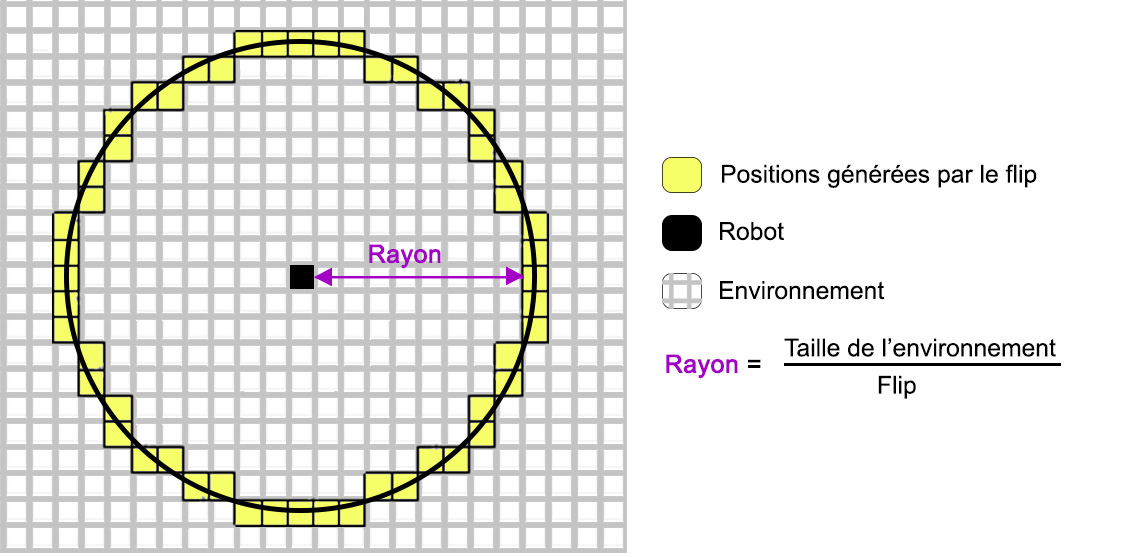
\includegraphics[width=0.7\textwidth]{flip.jpg}%
	\vspace{-0.1 cm}
	\captionof{figure}{Représentation de la méthode de génération de solutions avec le flip.}\label{flip}%
\end{center}



\subsection{MaxChance}
Une solution possède un nombre maximum de chances pour être sélectionnée comme solution de référence. Ce paramètre est aussi exploité afin de détecter la stagnation.

\subsection{Table Dance}
À chaque itération les abeilles déposent leurs meilleures solutions dans une table appelée \textit{"Table Dance"}. Cette table sera exploitée pour choisir la solution de référence de la prochaine itération. Ce choix se fait selon l'un des deux critères suivants:

\subsubsection{Critère de qualité (Best In Quality)}
Parmi les solutions présentes dans la table \textbf{Dance}, la meilleure en termes de qualité est celle possédant la valeur la plus élevée après évaluation.
Un exemple de sélection de la meilleure solution est illustré dans la figure \ref{bestQ} suivante:

\begin{center}	  
	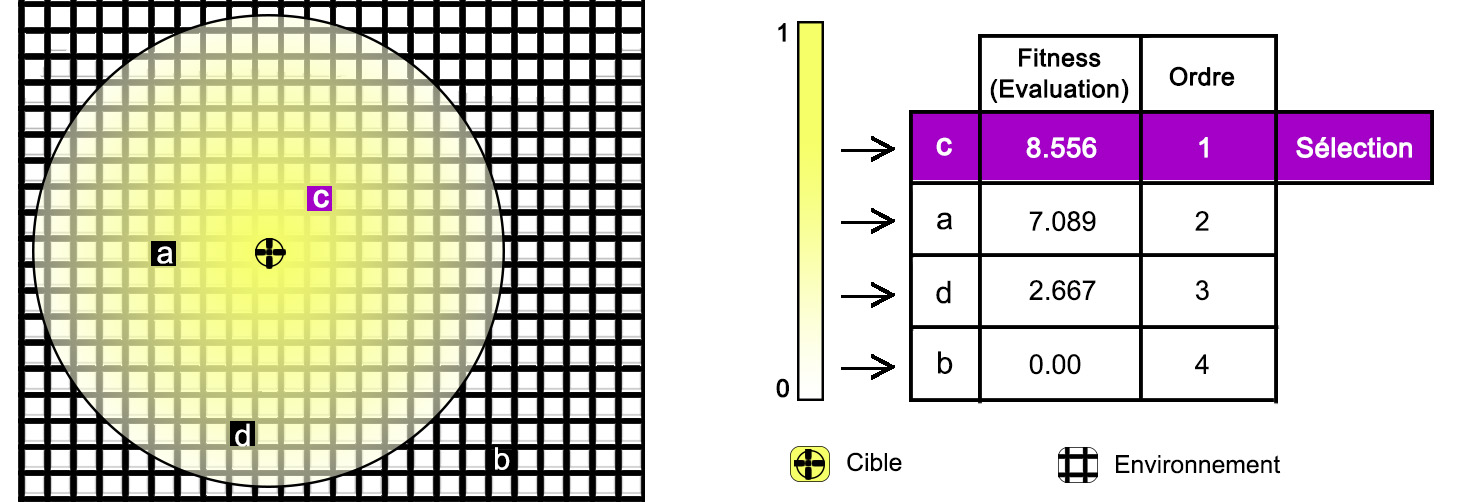
\includegraphics[width=0.85\textwidth]{BestQuality.jpg}%
	\vspace{-0.1 cm}
	\captionof{figure}{Méthode de sélection de la meilleure solution en termes de qualité.}\label{bestQ}%
\end{center}

\subsubsection{Critère de Diversité (Best In Diversity)}
En cas de stagnation, BSO  a recours au choix de la meilleure solution en termes de diversité appartenant à la table \textit{Dance} et ne figurant pas encore dans la liste \textit{Tabou}. Ce mécanisme permet l'exploration des zones distantes tout en évitant de tomber dans un minimum local.

Pour cela nous devons calculer la distance entre deux solutions, la formule choisie est la distance euclidienne, donnée comme suit:
\begin{equation}
Distance(S_1 , S_2) = \sqrt{(x_1 - x_2)^2 + (y_1 - y_2)^2}
\end{equation}

$S_1 :$ Solution 1 avec coordonnées ($x_1 , y_1$)

$S_2 :$ Solution 2 avec coordonnées ($x_2 , y_2$)\\

Le choix de la solution la plus diverse se fait en sélectionnant la solution dont la distance minimale par rapport aux autres solutions est maximale.
Cette méthode de sélection est schématisée dans la figure \ref{bestD} ci-contre:

\noindent
\begin{center}	  
	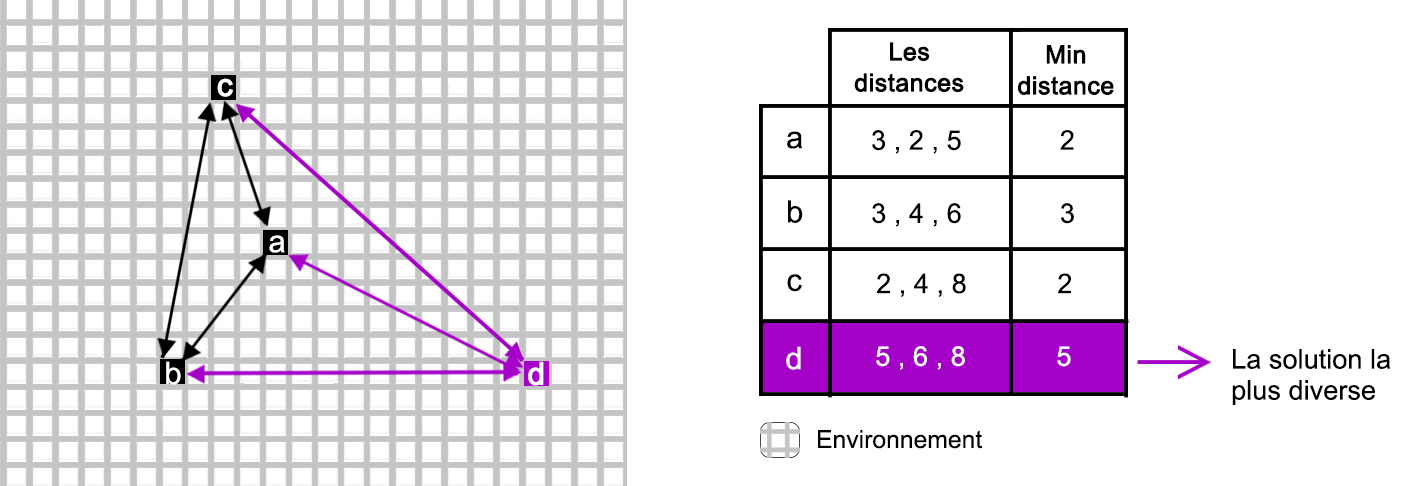
\includegraphics[width=0.9\textwidth]{BestDiversity.jpg}%
	\vspace{-0.1 cm}
	\captionof{figure}{Méthode de sélection de la meilleure solution en termes de Diversité.}\label{bestD}%
\end{center}




\textbf{ }\\

%\newpage

\section{Fonctionnement du Mono-BSO}
L’approche Mono-BSO est constituée d’un seul essaim d’abeilles où chaque robot se comporte comme une seule abeille. Les différentes étapes du Mono-BSO pour la recherche de cibles sont détaillées dans ce qui suit, suivi d'un organigramme \ref{monoBSO} résumant ces derniers.



\subsection{Initialisation de la solution de référence (Sref)}
Une solution (position(\textit{x,y})) est générée aléatoirement et conformément aux contraintes énoncées dans notre modélisation (voir section \ref{sol}).

\subsection{Insertion de Sref dans la liste \textit{Tabou}}
\label{etape2}
La solution de référence (Sref) de l'itération courante \textit{"t"} sera mise dans une liste \textit{Tabou} qu'on définit comme suit:
\paragraph{Liste Tabou }
Lorsqu'une position a déjà servi pour une abeille, nous gardons trace son passage dans la liste \textit{"Tabou"}, cela permet  de réduire la redondance (passage par les mêmes positions).  

\subsection{Génération des zones de recherche}
À partir de la solution de référence (Sref) on génère d'autres solutions, ces dernières déterminent des zones équidistantes de Sref. La génération de ces zones de recherche se fait grâce à l'opérateur \textbf{Flip}. 

\subsection{Affectation des zones aux abeilles}
Une fois les zones générées, on les affecte aux \textbf{"nbrBees"} abeilles de l'essaim de façon à ce que chaque abeille soit responsable de sa propre zone. 

\subsection{Recherche locale pour chaque abeille} 
Chaque abeille effectue une recherche locale qui consiste en l'évaluation d'une surface ronde de l'environnement dont le rayon est de vingt cases, cela constitue l'étape d'intensification. 

Dans le cas où la recherche locale apporte une amélioration, l'abeille prend cette nouvelle solution et réitère ce processus jusqu'à l'absence d'amélioration.

\subsection{Déplacement des abeilles}
Lors de la recherche locale, les abeilles peuvent trouver de meilleures solutions que celles qui leur ont été affectées, c'est pourquoi elles se déplacent vers ces solutions plus prometteuses dans l'environnement, ce qui simule le déplacement du robot. Chaque déplacement d'une position à une autre se fait à travers notre stratégie d'évitement d'obstacles (stratégie d'échantillonnage).


\subsection{Insertion des meilleures solutions dans la table \textit{Dance}}
Lorsqu'une abeille termine sa recherche locale elle communique sa meilleure solution au reste de l'essaim, cela en l'inscrivant dans la table \textit{Dance} commune à l'essaim.

Lorsqu'une cible est atteinte on incrémente le compteur relatif au nombre de cibles trouvées, si le nombre objectif de cibles \textbf{"nbrCible"} est égalé, la recherche prend fin avec succès.


\subsection{Choix de la nouvelle Sref}
Si à l'itération courant \textit{"t"} le nombre de cibles recherchées n'est pas atteint, une nouvelle solution de référence doit être choisie pour la prochaine itération.
 
Il existe alors deux critères possibles, le critère prioritaire est celui de qualité. 
Une solution prise selon le critère de qualité peut demeurer comme Sref au fil des itérations pour un nombre \textbf{"MaxChances"} de fois.
Dans le cas où toutes les chances données à cette Sref sont épuisées (stagnation), le choix de la nouvelle Sref se fera selon le second critère, celui de diversité.



\subsection{Critère d'arrêt de la recherche}
BSO continuera de réitérer les étapes citées plus haut à partir de \ref{etape2} jusqu'à à atteindre le nombre maximum d'itérations \textbf{"MaxIter"} ou le nombre de cibles recherchées \textbf{"nbrCible"}.



\paragraph{Remarque:}
Contrairement aux autres méta-heuristiques, BSO n'utilise pas seulement la fonction d'évaluation comme critère de sélection de solution, mais aussi la diversité. C'est un mécanisme pour remédier au problème de stagnation dans les minima locaux.



\noindent
\begin{center}
	\captionsetup{width=1\linewidth}
	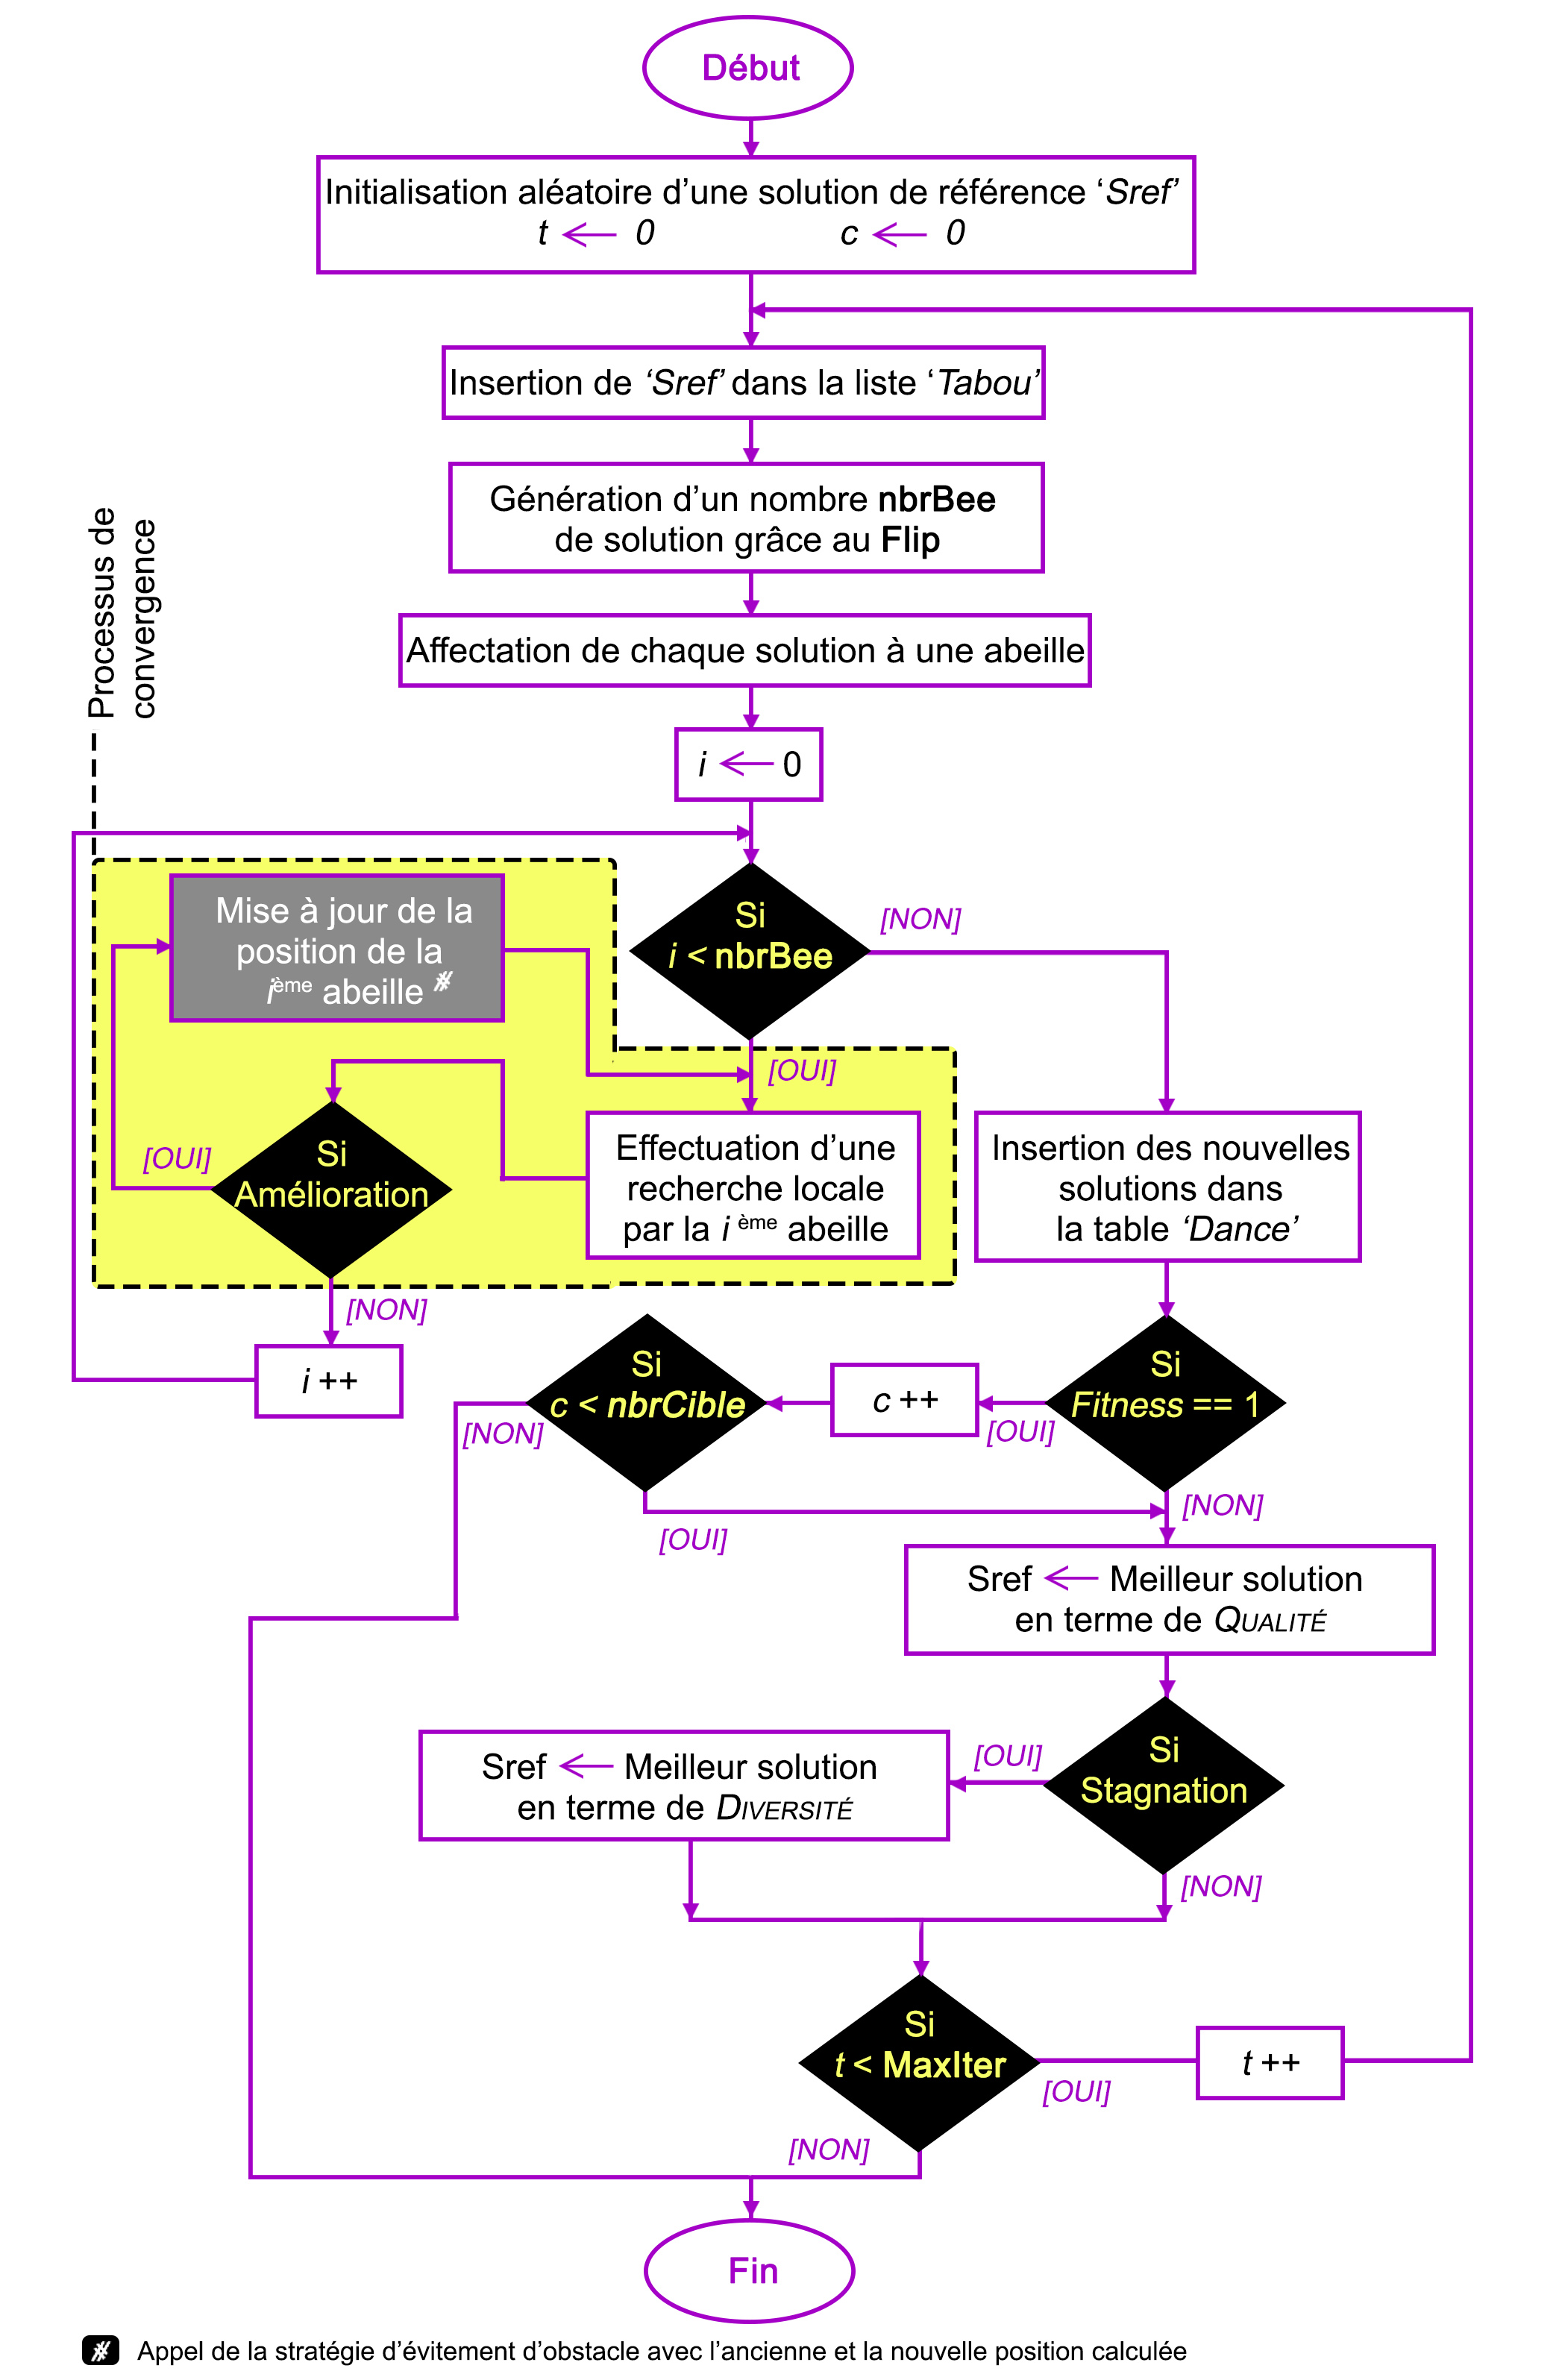
\includegraphics[width=1\textwidth]{mono-bso.jpg}%
	\vspace{-0.1 cm}
	\captionof{figure}{Organigramme du mode de fonctionnement de l'approche mono-BSO.}\label{monoBSO}%
\end{center}

\newpage

\section{Fonctionnement du Multi-BSO}
L’approche Multi-BSO quant à elle, consiste à associer à chaque robot, un essaim d’abeilles. Ils sont donc indépendants les uns des autres, mais ils sont en mode de coopération pour la recherche des cibles. Ils suivent le modèle d’interaction du tableau noir des systèmes multi-agents. Le processus de recherche de cibles implémenté à l’aide de Multi-BSO est décrit dans ce qui suit :

\subsection{Initialisation des solutions de référence (Srefs)} 
Un nombre \textbf{"nbrSwarm"} de solutions (x,y) est généré aléatoirement dans l'espace des solutions, de telle sorte à respecter les contraintes citées dans notre modélisation (voir section \ref{sol}).
Chaque position Sref est attribuée à un robot.


\subsection{Insertion de Sref dans la Liste Tabou}
Chaque essaim d'abeilles relatif à un robot dépose sa solution de référence (Sref) dans la liste \textit{Tabou}. Cette Liste \textit{Tabou} est commune à tous les robots, elle constitue leur moyen de communication (inter-essaim), permettant de réduire la redondance et repassage sur les mêmes solutions.

\subsection{Génération des zones de recherche }
À partir de la solution de référence (Sref) de chaque robot, les zones de recherche sont générées grâce à l'opération de \textbf{"Flip"}. Chaque zone est définie par une position dans l'espace de recherche.

\subsection{Affectation de chaque zone à une abeille }
Pour chaque robot disposant de \textbf{"nbrBees"} abeilles, chaque zone de recherche calculée précédemment est affectée à une abeille de son essaim, celle-ci y prend position.

\subsection{Recherche locale pour chaque abeille}
Chaque abeille effectue une recherche locale à partir de la zone qu'elle s'est vue affectée. Cette recherche consiste en l'évaluation des solutions (positions) de son voisinage à travers la fonction objectif.

À noter que tant qu'une abeille améliore la qualité de sa solution la recherche locale est réitérée de manière récursive.

\subsection{Insertion des solutions dans les tables \textit{Dance}}
Chaque essaim possède sa propre table \textit{Dance}, celle-ci permet la communication intra-essaim de telle sorte que chaque abeille y insère sa meilleure solution locale (de sa zone), afin d'en informer le reste de l'essaim. 


\subsection{Test de la $1^{\grave{e}re}$ condition d'arrêt}
Si une des abeilles a atteint une cible (solution optimale), le nombre de cibles trouvées \textit{"c"} est mis à jour. 
Dans le cas où le nombre de cibles recherchées \textbf{"nbrCible"} est égalé, alors la mission touche à sa fin.

\subsection{Choix de la nouvelle solution de référence}
À priori, la meilleure solution en matière de qualité est sélectionnée à partir de la table \textit{Dance} comme nouvelle solution de référence (Sref).
Sauf en cas de stagnation où une même solution est prise pour solution de référence au-delà de \textbf{"MaxChances"} fois, Sref est alors choisie selon le critère de diversité.


\subsection{Déplacement des robots}
Chaque robot se déplace de son ancienne position vers la nouvelle position calculée (Sref) en employant notre stratégie d'évitement d'obstacles.


\subsection{Test de la $2^{\grave{e}me}$ condition d'arrêt}
Le nombre d'itérations \textit{"t"} est incrémenté puis comparé au nombre maximum d'itérations \textbf{"MaxItér"} accordé à la recherche.\\



L'approche Multi-BSO peut alors être perçue comme l'application de Mono-BSO par chaque robot. L'organigramme de son fonctionnement est résumé dans la figure ci-contre.
\noindent
\begin{center}	  
	\captionsetup{width=1\linewidth}
	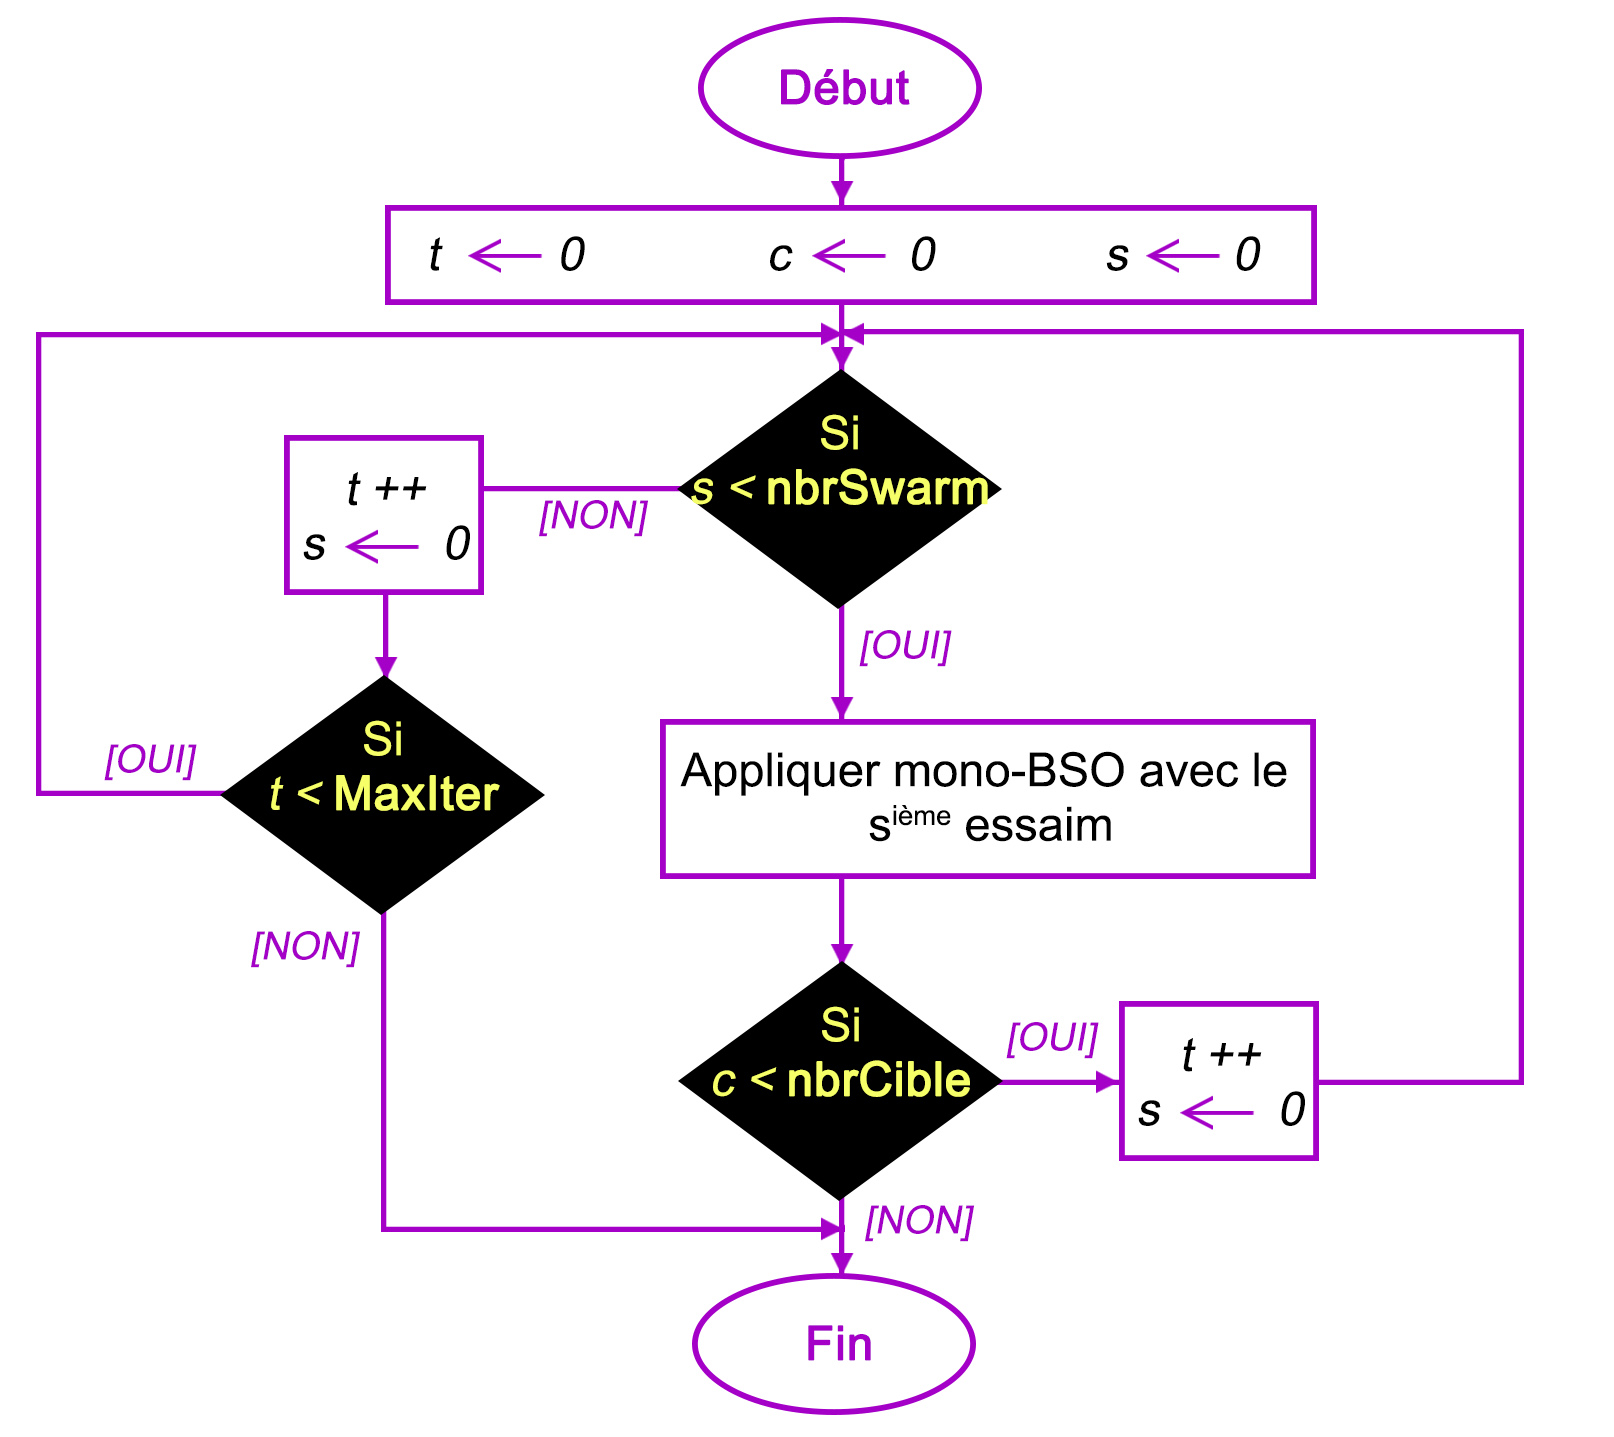
\includegraphics[width=0.7\textwidth]{multi-bso.jpg}%
	\vspace{-0.3cm}
	\captionof{figure}{Organigramme du mode de fonctionnement de l'approche multi-BSO.}\label{multiBSO}%
\end{center}


\section{Conclusion}
À travers ce chapitre, on a pu mettre en évidence deux approches inspirées du comportement des abeilles BSO et Multi-BSO. Ces algorithmes intelligents reposent sur les mêmes paramètres et fonctions de base, mais avec un mode d'emploi légèrement différent pour Multi-BSO qui nécessite la coordination des essaims (équipes) d'abeilles.

Tout en restant dans la même dynamique des techniques inspirées des comportements d'animaux, nous nous penchons dans le chapitre suivant sur deux approches simulant le comportement des éléphants, qui sont très différents des abeilles de part leurs tailles et mécanismes sociaux.







\chapter{Chapitre 5 : Algorithmes des éléphants pour le problème de recherche de cibles}

\label{Chapter5}

\section{Introduction}
La deuxième contribution majeure de ce projet est l'adaptation des deux algorithmes basés
essaim d'éléphants vus précédemment, à savoir EHO et ESWSA pour le problème de la
recherche de cibles.
Il sera question dans ce chapitre d'effectuer une adaptation de l'ensemble des concepts de ces deux méthodes de résolution à la modélisation exhibée au niveau du chapitre 3, ainsi que les différentes étapes de leur fonctionnement. 


\section{Adaptation de EHO pour le problème de la recherche de cibles}
L'algorithme EHO fut présenté de manière générale au niveau du chapitre 2, nous allons maintenant nous intéresser à son adaptation au problème de recherche de cibles. Les aspects phares de cette approche seront redéfinies comme suit :


\subsection{Solution}
Une solution est la position de coordonnées \textit{(x, y)} dans laquelle se trouve un éléphant.

\subsection{Fonction objectif}
La fonction objectif est comme définie pour l'approche BSO, à la différence près que pour EHO ce sont les éléphants qui sont responsables de l'évaluation des solutions.


\subsection{Éléphant}
Un éléphant est un robot, il occupe une case unique dans l'environnement à chaque instant \textit{"t"}. La mise à jour de la position d'un éléphant par rapport à son clan suit l'équation \ref{eq:xnew} pour les deux dimensions \textit{(x,y)}, comme suit :
\begin{equation}
\begin{split}
{x}_{new,c,i} = {x}_{c,i} + \alpha *( {x}_{Best,c} - {x}_{c, i} ) * r \\
{y}_{new,c,i} = {y}_{c,i} + \alpha *( {y}_{Best,c} - {y}_{c, i} ) * r 
\end{split}
\end{equation}

La figure \ref{elephant} ci-dessous représente l'influence de la meilleure solution sur le déplacement des autres éléphants du clan selon différents degrés $\alpha$.
\begin{center}	  
	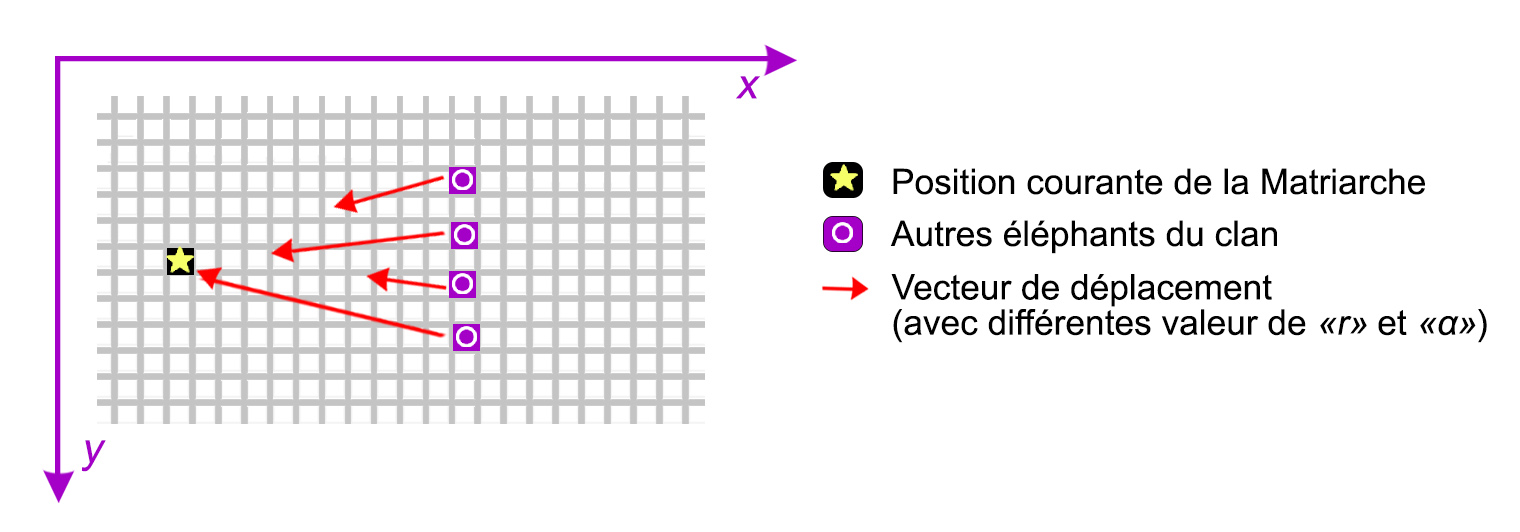
\includegraphics[width=0.9\textwidth]{elephant.jpg}%
	\vspace{-0.3cm}
	\captionof{figure}{Représentation de la méthode de mise à jour des positions des éléphants.}\label{elephant}%
\end{center}

\subsection{Clan}
\label{clanArea}
Les éléphants d'un même clan sont généralement regroupés dans une même zone. Ainsi, les positions initiales des éléphants sont générées comme suit:
\begin{enumerate}
	\item Pour chaque clan générer une position initiale aléatoirement.
	\item À partir de chaque position générée, positionner les \textbf{nbrElephant} - 1 autres éléphants sur une surface ronde de rayon inférieur ou égale à une certaine limite (5 cases dans notre cas).
\end{enumerate}
La figure \ref{clan} ci-dessous, représente un exemple de positions générées pour les éléphants d'un même clan :
\begin{center}	  
	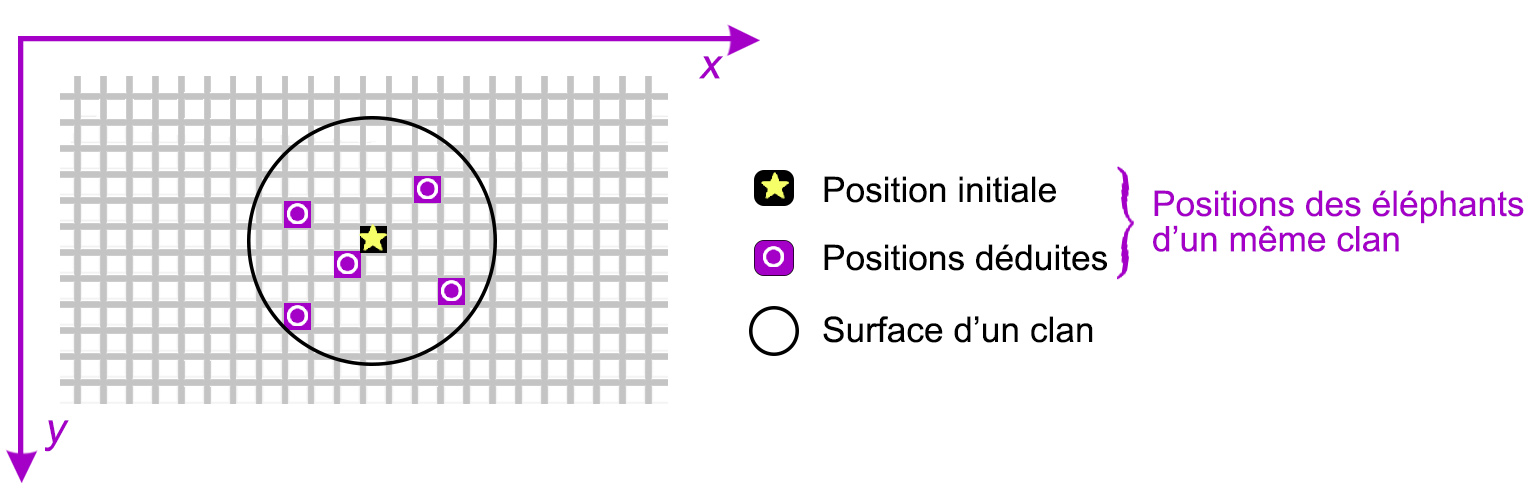
\includegraphics[width=0.95\textwidth]{Clan.jpg}%
	\vspace{-0.1 cm}
	\captionof{figure}{Représentation de la technique de génération des positions des éléphants d'un même clan.}\label{clan}%
\end{center}

\subsection{Chef de clan (Matriarche) }
L'éléphant chef de clan appelé "Matriarche" est celui qui possède la meilleure solution de son clan. La mise à jour de cette position dépend du centre de gravité du clan, comme présentée dans l'équation \ref{eq:xbest}, elle est appliquée de la même manière à chacune des coordonnées \textit{x} et \textit{y}, comme suit :
\begin{equation}
\begin{split}
{x}_{Best,c} = \beta  *  {x}_{center,c} \\
{y}_{Best,c} = \beta  *  {y}_{center,c}  
\end{split}
\end{equation}

De même, le centre de gravité est calculé pour les deux dimensions, par l'équation:
\begin{equation}
	\begin{split}
	{x}_{center,c}  = \frac{1}{N} * \sum_{i=1}^{N} {x}_{c,i}\\
	{y}_{center,c}  = \frac{1}{N} * \sum_{i=1}^{N} {y}_{c,i}
	\end{split}
\end{equation}

La figure \ref{chef} montre le processus de mise à jour de la position de la "Matriarche".

\begin{center}	  
	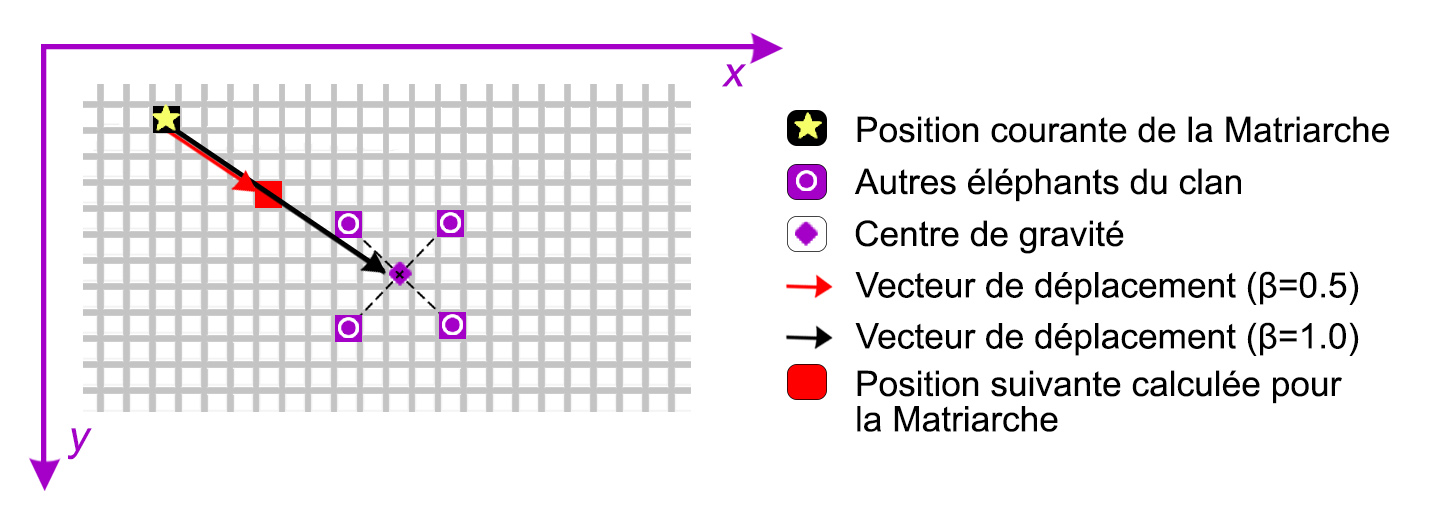
\includegraphics[width=0.95\textwidth]{chefClan.jpg}%
	\vspace{-0.1 cm}
	\captionof{figure}{Représentation de la méthode de mise à jour de la position du meilleur éléphant/robot.}\label{chef}%
\end{center}

\subsection{Éléphant mâle}
Dans chaque clan, l'éléphant évalué comme détenant la pire solution est appelé \textit{"pire éléphant"}. Il possède une fonction de mise à jour particulière décrite par l'équation \ref{eq:xworst}, qui pour notre environnement 2D de taille $taille_{Coté}$ est adaptée par l'équation :
\begin{equation}
\begin{split}
{x}_{Worst,c}  =  (taille_{Cot\acute{e}} - 1) * rand \\
{y}_{Worst,c}  =  (taille_{Cot\acute{e}} - 1) * rand 
\end{split}
\end{equation}

Celle-ci favorise la diversification afin d'explorer une plus grande surface de l'environnement.
Un exemple d'application de cette équation est présenté dans la figure \ref{worst} qui suit :

\begin{center}	  
	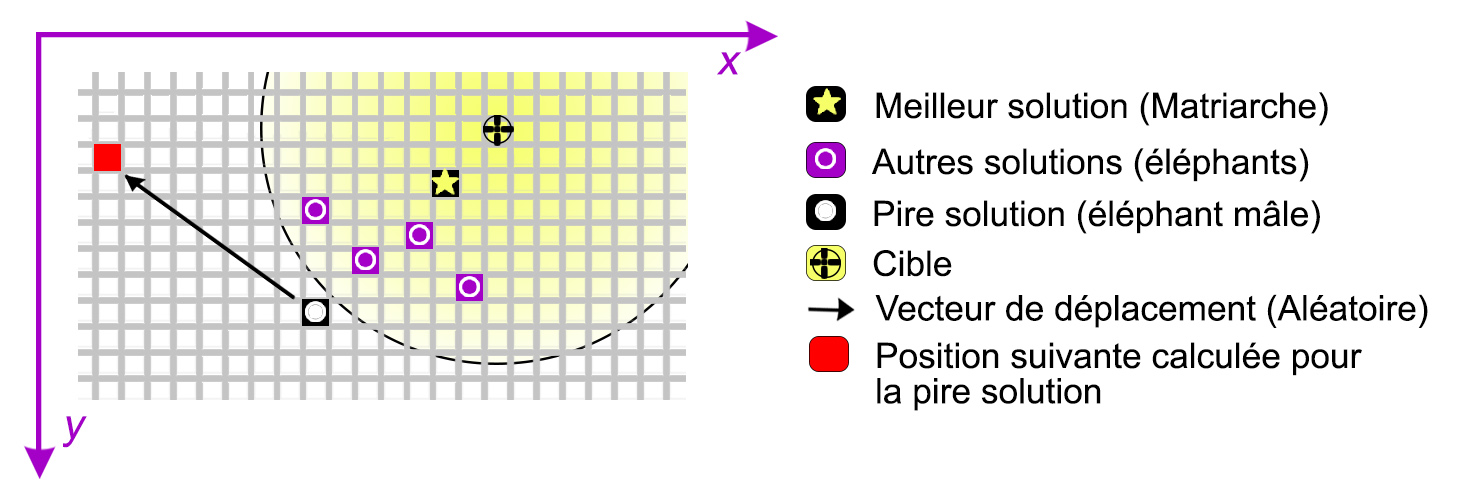
\includegraphics[width=0.95\textwidth]{worst.jpg}%
	\vspace{-0.1 cm}
	\captionof{figure}{Représentation de la méthode de mise à jour de la position du pire éléphant/robot.}\label{worst}%
\end{center}



%\newpage

\section{Fonctionnement d'EHO}
La méthode EHO repose sur la présence de plusieurs clans de robots éléphants, où chaque clan possède un chef aussi appelé \textit{"meilleur éléphant"} ou \textit{"Matriarche"} et un pire éléphant devant se séparer du clan. Les différents clans coopèrent dans le but commun de recherche de cibles. Deux types de communication sont utilisés, d'abord la communication entre robots d'un même clan sur les meilleures solutions trouvées, en second lieu la communication entre clans relative au nombre de cibles, celle-ci faisant office de tableau noir. L'organigramme de la figure \ref{eho} décrit son fonctionnement.

\subsection{Initialisation des positions des clans}
Pour commencer, nous initialisons les positions des \textbf{"nbrClan"} clans de manière aléatoire dans notre espace des solutions, en tenant compte des contraintes concernant les bornes et les obstacles de ce dernier.

\subsection{Initialisation des positions des éléphants}
À partir des positions des clans, sont déduites les positions des \textbf{"nbrEle"} éléphants de chaque clan comme décrit dans la section \ref{clanArea}.



\subsection{Évaluation des solutions }
\label{eval}
Chaque clan \textit{"Cl"} se voit évaluer les solutions que portent tous ses éléphants.
Dès qu'une nouvelle cible est trouvée, le nombre de cibles détectées \textit{"c"} est incrémenté. Ainsi, si le nombre total de cibles \textbf{"nbrCible"} de notre environnement est atteint, la mission de recherche est un succès et donc interrompue.

\subsection{Tri des clans}
Chaque clan parmi les \textbf{"nbrClan"}, procède au tri de ses éléphants selon la fonction objectif dans l'ordre décroissant de ses valeurs.

\subsection{Mise à jour des positions des éléphants}
Pour chaque éléphant \textit{"ele"} du clan \textit{"Cl"} on détermine la nouvelle position. Pour cela, les deux paramètres nécessaires sont la position du chef de clan et le paramètre empirique $\alpha$.\\

La nouvelle position du meilleur éléphant de chaque clan est calculée à partir du centre de gravité du clan $CG_{Cl}$ et du paramètre empirique $\beta$.\\

La génération de la prochaine position du pire éléphant de chaque clan grâce à l'opérateur de séparation de base aléatoire.

\subsection{Déplacement des robots}
Chaque robot éléphant \textit{"ele"} se déplace vers la nouvelle position calculée via notre processus d'évitement d'obstacles.


\subsection{Test de la condition d'arrêt}
Incrémenter le nombre d'itérations effectuées \textit{"t"}.
Le processus de recherche prend fin si le nombre maximum d’itérations \textbf{"MaxIter"} est atteint. Dans le cas contraire, le processus reprend à partir de l'étape d'évaluation des solutions (section \ref{eval}). 
	


\noindent

\begin{center}	  
	\captionsetup{width=1\linewidth}
	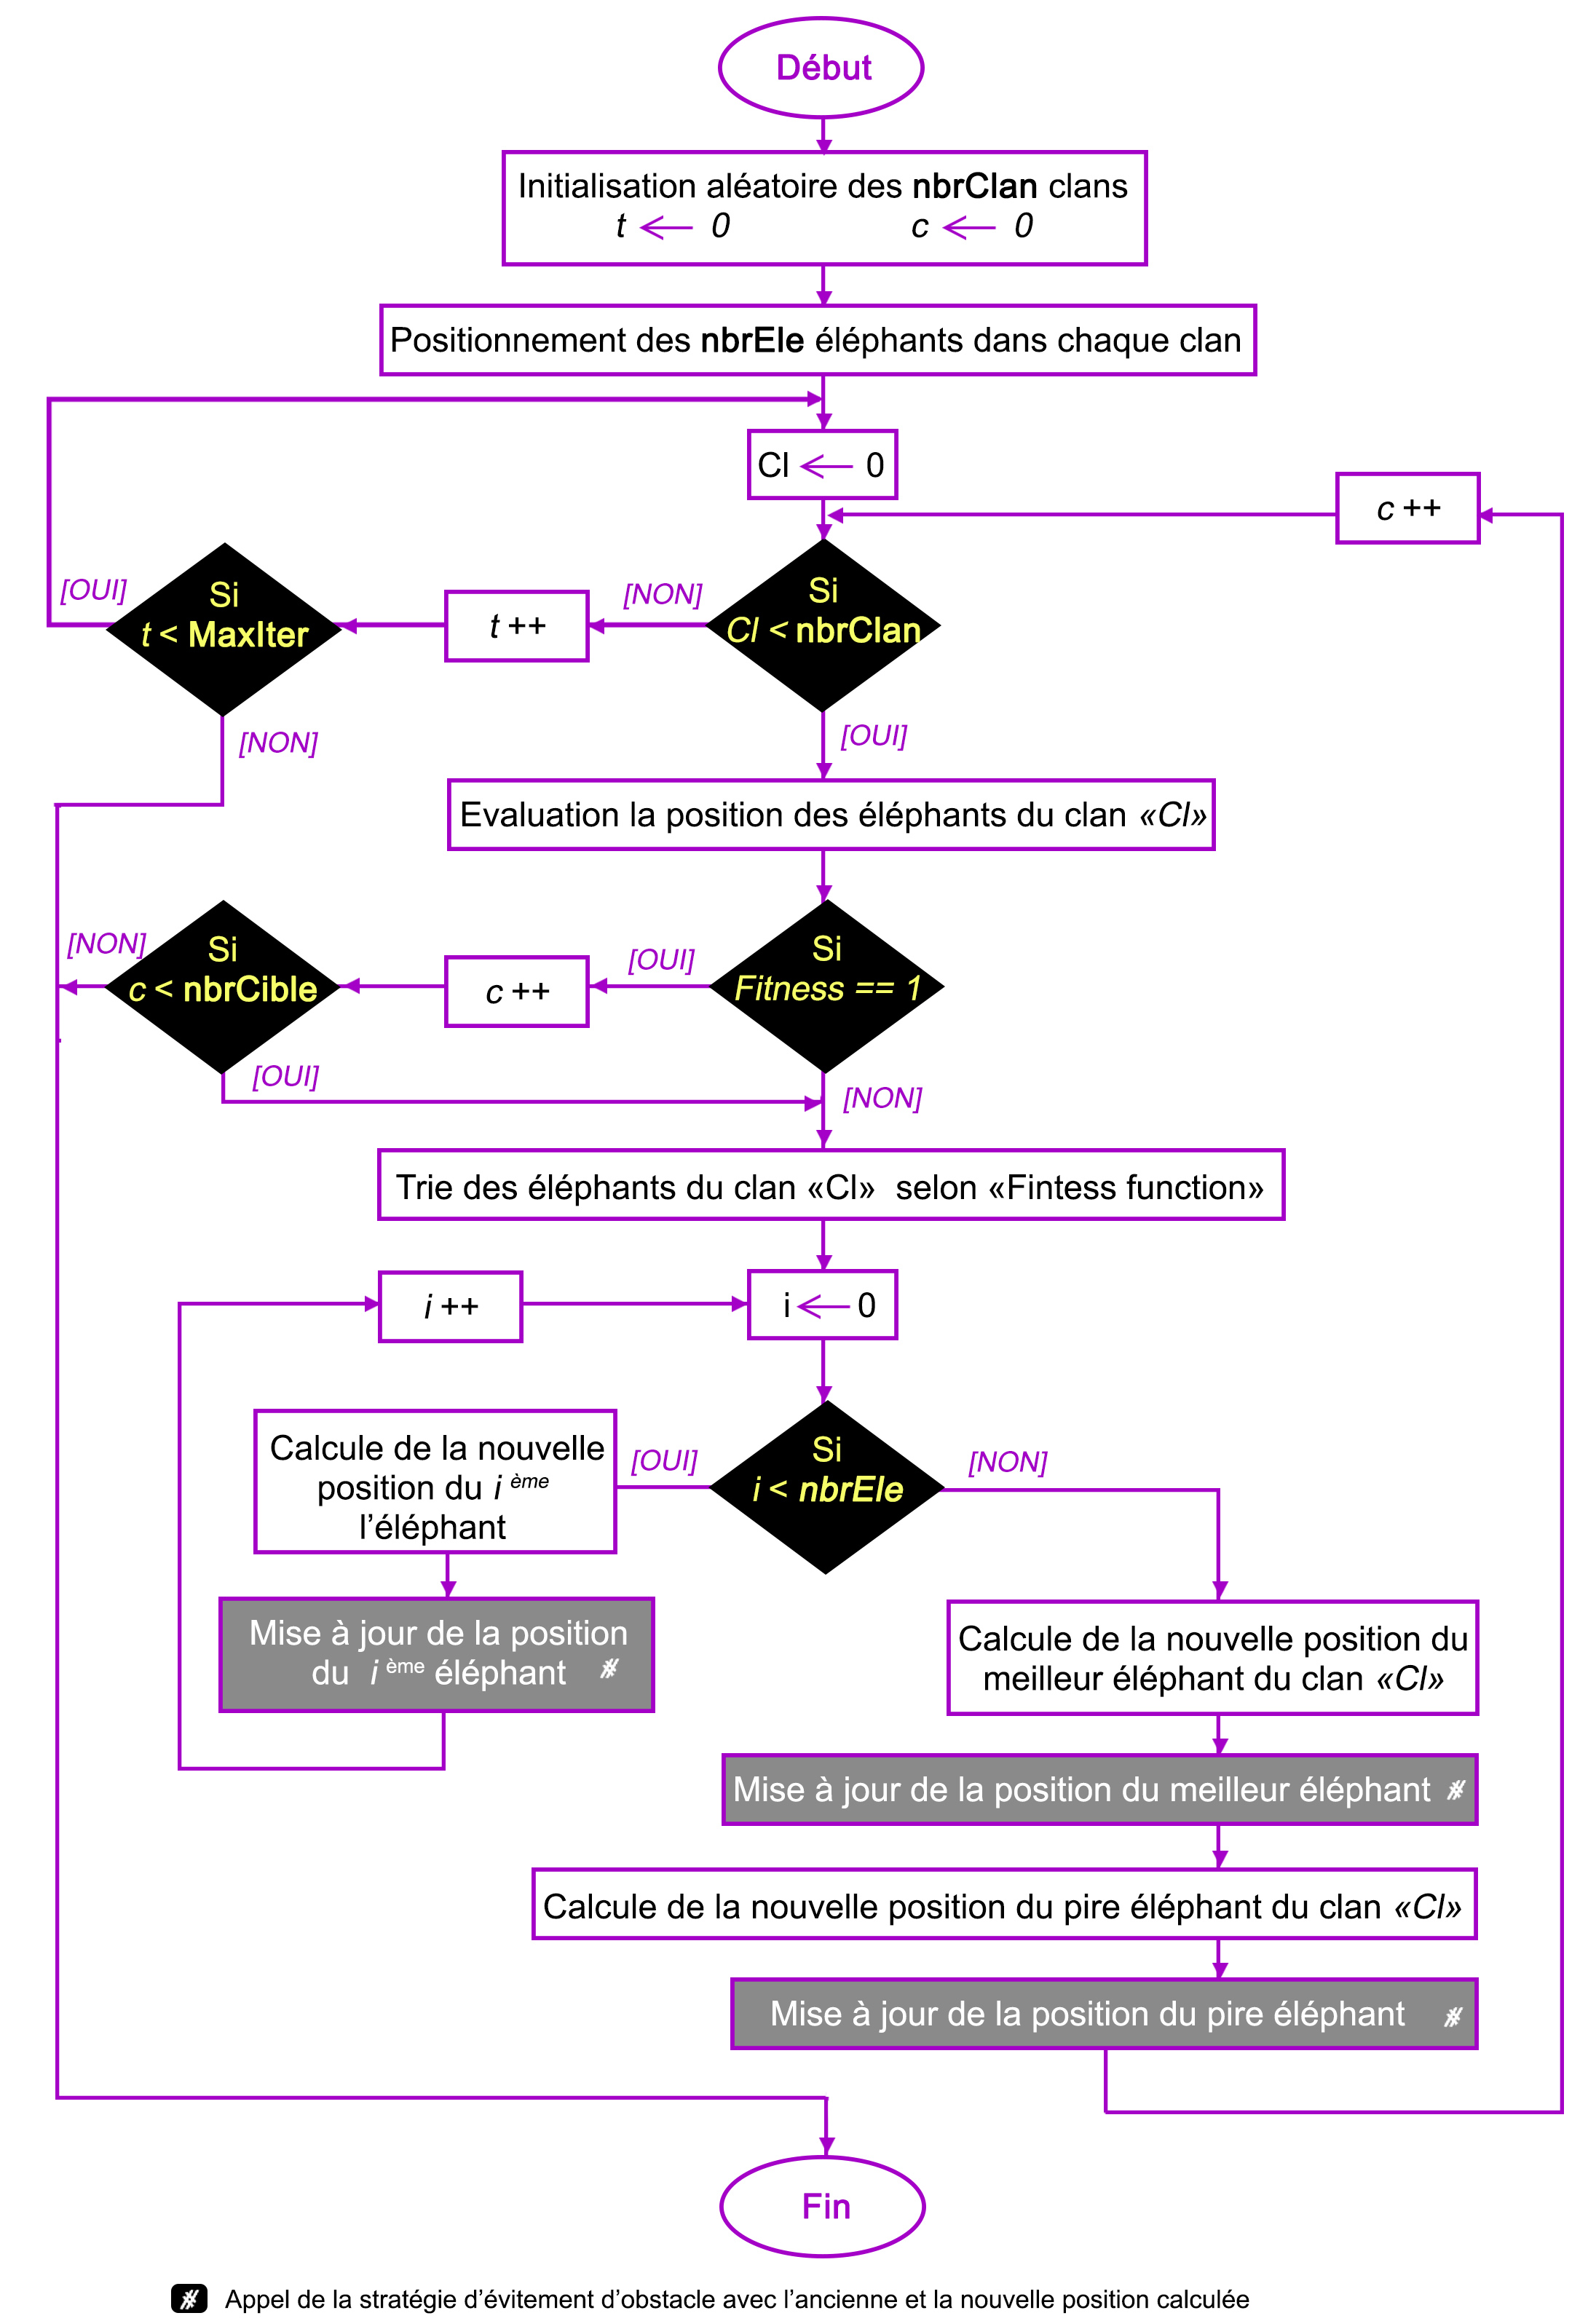
\includegraphics[width=0.95\textwidth]{eho.jpg}%
	\vspace{-0.1 cm}
	\captionof{figure}{Organigramme du mode de fonctionnement de l'approche EHO.}\label{eho}%
\end{center}



\newpage

\section{Adaptation de ESWSA pour le problème de la recherche de cibles}
\subsection{Solution}
Tout comme EHO, une solution pour ESWSA est la position de coordonnées \textit{(x, y)} occupée par un éléphant se comportant comme un robot.

\subsection{Fonction objectif}
La fonction objectif est la même que pour EHO, où les éléphants sont responsables de l'évaluation des solutions.


\subsection{Éléphant}
Un éléphant simule un robot, il occupe une case dans la grille de l'environnement. Il est doté d'une mémoire qui englobe sa meilleure position personnelle "$pbest$" et la meilleure position globale "$gbest$" du groupe d'éléphants.
La dimension du vecteur de positions est alors égale à deux.
\begin{equation}
X_{i,2} = (x_{i1},x_{i2})
\end{equation}
Pour des soucis de compréhension on a choisi la notation $(x,y)$ avec $i$ l'identifiant de l'éléphant
\begin{equation}
X_{i,2} = (x_{i},y_{i})
\end{equation}

\subsection{Outils de mémoire}
\label{Pbest} \textbf{"Pbest"} dite \textbf{"personal best"}, spécifique à chaque éléphant de l’essaim. Elle représente la position de l’éléphant dans l’environnement qui a maximisé la fonction objectif tout au long de la recherche. C'est la meilleure solution en qualité de l’éléphant.
%celle qui est la plus proche d'une cible particulière étant par conséquent 
\begin{equation}
\begin{split}
Pbest_{i}= &(Pbest_{xi},Pbest_{yi})\\
Pbest^{t}_{i}=&\max\limits_{1 \leq j\leq t}(f(X^{j}_{i}))
\end{split}
\end{equation}

La mise à jour du \textit{Pbest} d'un éléphant au fil des itérations est représentée dans la figure \ref{pbest} suivante :
\noindent
\begin{center}	  
	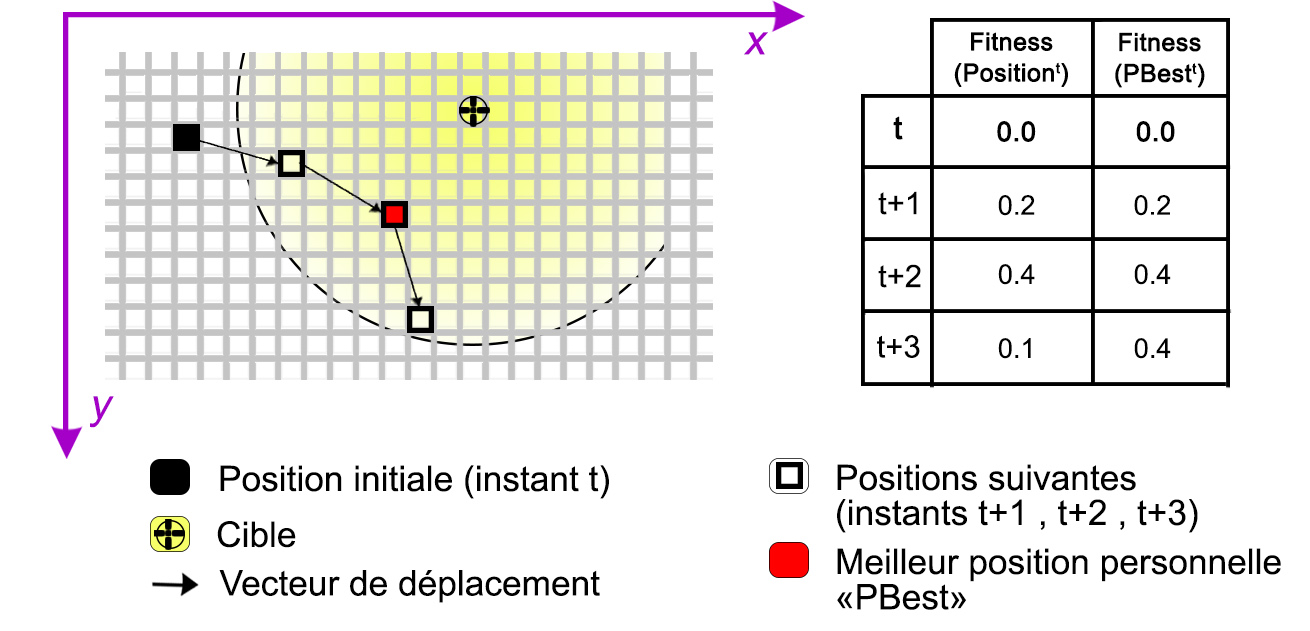
\includegraphics[width=0.9\textwidth]{PBest.jpg}%
	\vspace{-0.1 cm}
	\captionof{figure}{Représentation de la méthode de mise à jours du Pbest d'un éléphant.}\label{pbest}%
\end{center}


\textbf{Global best} (\label{Gbest}) ou encore meilleure position globale, est une position spécifique à l'essaim, c'est la meilleure position trouvée par tout l'essaim. 
%et par conséquent la plus proche par d'une certaine cible de tout l’essaim. 
On peut dire que le \textit{Gbest} consiste à trouver le max en termes de qualité des \textit{Pbest} de chaque éléphant, comme le montre l'équation suivante :

\begin{equation}
\begin{split}
Gbest= &(Gbest_{x},Gbest_{y})\\
Gbest^{t} = & \max(f(Pbest^{t}_{i}))
\end{split}
\end{equation}
Chaque éléphant a connaissance de la valeur du Gbest à chaque itération, c'est une connaissance commune à tous.

\subsection{Vélocité}
La vélocité combine la vitesse et la direction qui détermine la prochaine position de l'éléphant. La notation de la vélocité dans un environnement bidimensionnel est la suivante :
\begin{equation}
\begin{split}
V_{i,2}= & (v_{xi},v_{yi})\\
\end{split}
\end{equation}

\subsection{Mécanisme de déplacement}
\subsubsection{Mise à jour de la vélocité de l'éléphant}
La mise à jour de la vélocité est sujette à plusieurs paramètres dont les positions $Pbest$ et $Gbest$. Comme on peut le voir dans la figure \ref{velocity}, d'après la constante $p$ l'éléphant choisira de suivre sa meilleure position ou la meilleure du groupe, ce qui lui évite de stagner dans des optimums locaux.

\noindent
\begin{center}	  
	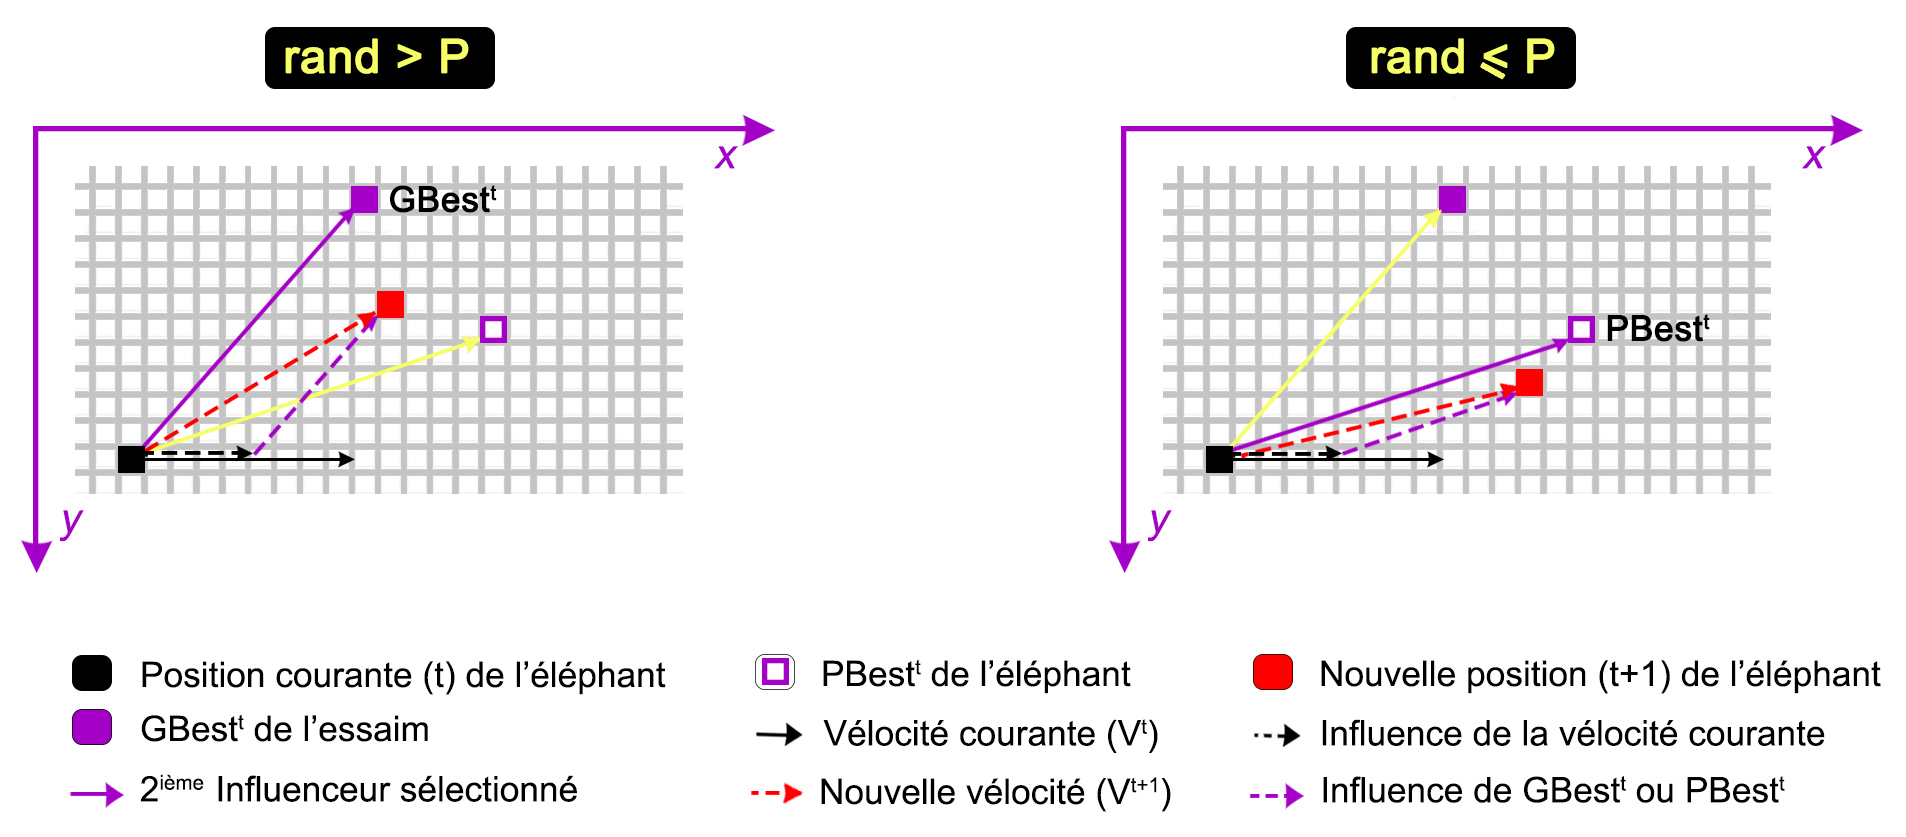
\includegraphics[width=1\textwidth]{deplacement-eswsa.jpg}%
	\vspace{-0.1 cm}
	\captionof{figure}{Représentation de la mise à jour de la vélocité d'un éléphant dans l'approche ESWSA.}\label{velocity}%
\end{center}

Vu qu'on se trouve dans un environnement bidimensionnel, on doit calculer deux vélocités, une selon les abscisses et une selon les ordonnées, ce processus est explicité dans les deux équations qui suivent:
%Le calcul de celle des abscisses se fait avec la première composante des positions $X_{i,2}$, $P_{best,i,2}$ , $G_{best,2}$, alors que celle des ordonnées se fait avec leur seconde composante. On explicite dans les deux équations qui suivent le calcul de la vélocité.
\begin{equation}
v_{xi}^{t+1}=
\left\lbrace
\begin{array}{ccc}
v_{xi}^{t} * w^t + rand * (Gbest_{x}^{t} - x_{i}^{t} ) & \mbox{si} & random > p\\
v_{xi}^{t} * w^t + rand * (Pbest_{xi}^{t} - x_{i}^{t} )  & \mbox{si} & random \leq p
\end{array}\right.
\end{equation}

\begin{equation}
v_{yi}^{t+1}=
\left\lbrace
\begin{array}{ccc}
v_{yi}^{t} * w^t + rand * (Gbest_{y}^{t} - y_{i}^{t} ) & \mbox{si} & random > p\\
v_{yi}^{t} * w^t + rand * (Pbest_{yi}^{t} - y_{i}^{t} )  & \mbox{si} & random \leq p
\end{array}\right.
\end{equation}
Notre environnement a des bornes fixes, cette formule de calcul risque de générer des vélocités trop grandes ce qui perturbe l'organisation et le comportement du groupe d'éléphants. Une solution est de borner la vélocité.
Soient les bornes de l'environnement représentées par le point $MaxP$
\begin{equation}
\begin{split}
MaxP= &(MaxP_{x},MaxP_{y})\\
v_{xi}^{t+1}=&v_{xi}^{t+1} \bmod MaxP_{x}\\
v_{yi}^{t+1}=&v_{yi}^{t+1} \bmod MaxP_{y}
\end{split}
\end{equation}






\subsubsection{Mise à jour de la position de l'éléphant}
Tout comme la \label{vélocité} la mise à jour de la position $X_{i,2}$ de l'éléphant $i$ se fait sur deux niveaux celui des abscisses et celui des ordonnées, l'équation de mise à jour est la suivante : 
\begin{equation}
\begin{split}
x_{i}^{t+1} & = v_{xi}^{t+1} + x_{i}^{t}\\
y_{i}^{t+1} & = v_{yi}^{t+1} + y_{i}^{t}
\end{split}
\end{equation}
Toujours pour éviter les valeurs aberrantes, on procède de la même manière qu'avec la vélocité en bornant la position, soit :
\begin{equation}
\begin{split}
MaxP= &(MaxP_{x},MaxP_{y})\\
x_{i}^{t+1}= & x_{i}^{t+1} \bmod MaxP_{x}\\
y_{i}^{t+1}= & y_{i}^{t+1} \bmod MaxP_{y}
\end{split}
\end{equation} 

Ainsi, la position de l'éléphant est calculée en tenant compte de sa connaissance de sa position à l'instant $t$ afin de calculer celle de l'instant $t+1$.





\subsubsection{Mise à jour de $W^t$ (poids d'inertie)}
Le poids d'inertie est un paramètre qui influence la vélocité et ainsi le calcul des positions des éléphants. Comme on a pu le voir dans le chapitre 2  section ~\ref{LDIW} page ~\pageref{LDIW}, l'équation choisie calcule le poids d'inertie selon le nombre d'itérations $t$
avec l'initialisation suivante :
\begin{equation}
\begin{split}
W_{max}= & 0.9\\
W_{min}= & 0.1\\
t_{max}= & 1000\\
W^{t} = & W_{max} - \frac{W_{max} - W_{min}}{t_{max}} * t
\end{split}
\end{equation}
$W^t$ joue un rôle important dans la convergence des éléphants vers la solution optimale, il détermine le taux de vélocité mémoire. C'est-à-dire la vélocité à l'instant $t$, qui influencera la prochaine vélocité à l'instant $t+1$.
Il permet alors de contrôler et varier la vitesse et la trajectoire afin d'explorer au mieux l'environnement de recherche.\\






\section{Fonctionnement d'ESWSA}
Dans ESWSA, chaque éléphant se comporte comme un robot indépendant du groupe mais coopératif. Doté d'une mémoire qui se présente en sa $pbest$ et $gbest$ qui sont nécessaires pour le choix des trajectoires possibles. L'organisation des éléphants lors de la recherche suit un schéma dont on explicite les étapes dans la figure \ref{eswsa} et dans le processus suivant :



\subsection{Initialisation}
Comme toute méta-heuristique, ESWSA commence par une étape d'initialisation déterminante pour le bon déroulement de la recherche à savoir :
\subsubsection{Paramètres empiriques}
Initialiser les paramètres empiriques consiste à leur choisir des valeurs fixes. Ils sont souvent le sujet d'un réglage pour augmenter l'efficacité et performance des approches basées essaim. Les paramètres d'ESWSA sont : 
\textit{Tmax, nbrEle, P, $W^t$, MaxP, MinP.}

\subsubsection{Positions initiales des éléphants}
L'emplacement initial des éléphants est aussi un facteur influent de la recherche. On initialise chaque éléphant à une position aléatoire en respectant les contraintes énoncées dans le chapitre 3.

\subsubsection{Pbest pour chaque éléphant}
Après avoir choisi les positions des éléphants, on doit évaluer la qualité de cette position. Cette évaluation permet d'initialiser les $Pbest$ (Meilleure position personnelle en termes de qualité) de chaque éléphant de l'essaim.

\subsubsection{Gbest}
Comme on a pu l'expliquer plus haut dans \ref{Gbest}, la position \textit{Gbest} (Meilleure position globale de tout l'essaim) est initialisée selon le maximum des positions $pbest$ évaluées en termes de qualité. En d'autres termes, celle qui détient la valeur maximum de la fonction objectif.

Une fois les initialisations faites, le processus d'ESWSA se met en marche selon ce qui suit :

\subsection{Mise à jour de la vélocité pour chaque éléphant}
Chaque éléphant de l'essaim se voit mettre à jour sa vélocité, cela se fait avec \textit{le choix d'un nombre aléatoire} qui détermine l'équation à choisir. Si ce nombre aléatoire est inférieur au paramètre empirique \textit{p} alors la vélocité sera calculée par rapport à sa position $Pbest$, sinon ça sera d'après le $Gbest$. Autrement dit l'éléphant choisira de privilégier le suivi de sa position $Pbest$ ou bien $Gbest$ à chaque itération.

\subsection{Calcul de la prochaine position de chaque éléphant}
Une fois la vélocité calculée, elle nous permet de mettre à jour la position de chaque éléphant selon l'équation de mise à jour voir section \ref{vélocité}.
%, en additionnant la vélocité à la position précédente de l'éléphant.

\subsection{Déplacement des robots}
Vu qu'un éléphant simule un robot, son déplacement se fait en employant la stratégie d'évitement d'obstacles, en cas d'environnement à obstacles.

\subsection{Évaluation des positions des éléphants}
Un éléphant a un angle de vue lui permettant de voir autour de lui sur une superficie de dix cases, ces cases seront évaluées selon la fonction objectif. L'éléphant gardera la position de la meilleure case.

Si une cible est détecté, le nombre de cibles trouvées \textit{"c"} est alors incrémenté.

\subsection{Mise à jour du Pbest de chaque éléphant}
Pendant la recherche, la position $Pbest$ est susceptible de changer, c'est pourquoi après chaque évaluation un test est effectué pour savoir si la mise à jour du $Pbest$ de l'éléphant est nécessaire. Ça signifie qu'on a trouvé une meilleure position nous rapprochons d'une cible.

\subsection{Mise à jour de Gbest}
Après l'éventuelle mise à jour des positions $Pbest$, vient la mise à jour de la position $Gbest$, où un test est effectué également pour un potentiel changement du $Gbest$.

\subsection{Mise à jour du $W^t$ (poids d'inertie)}
Le poids d'inertie est relatif à chaque itération dont on calcule la valeur selon l'itération courante.

\subsection{Critère d'arrêt de la recherche}
Le processus d'ESWSA s'exécute en boucle, en incrémentant le nombre d'itérations \textit{"t"},  jusqu'à la rencontre de toutes les \textbf{"nbrCible"} cibles ou bien jusqu'à atteindre le nombre maximum d'itérations \textbf{"MaxIter"}. 


\noindent
\begin{center}	  
	\captionsetup{width=1\linewidth}
	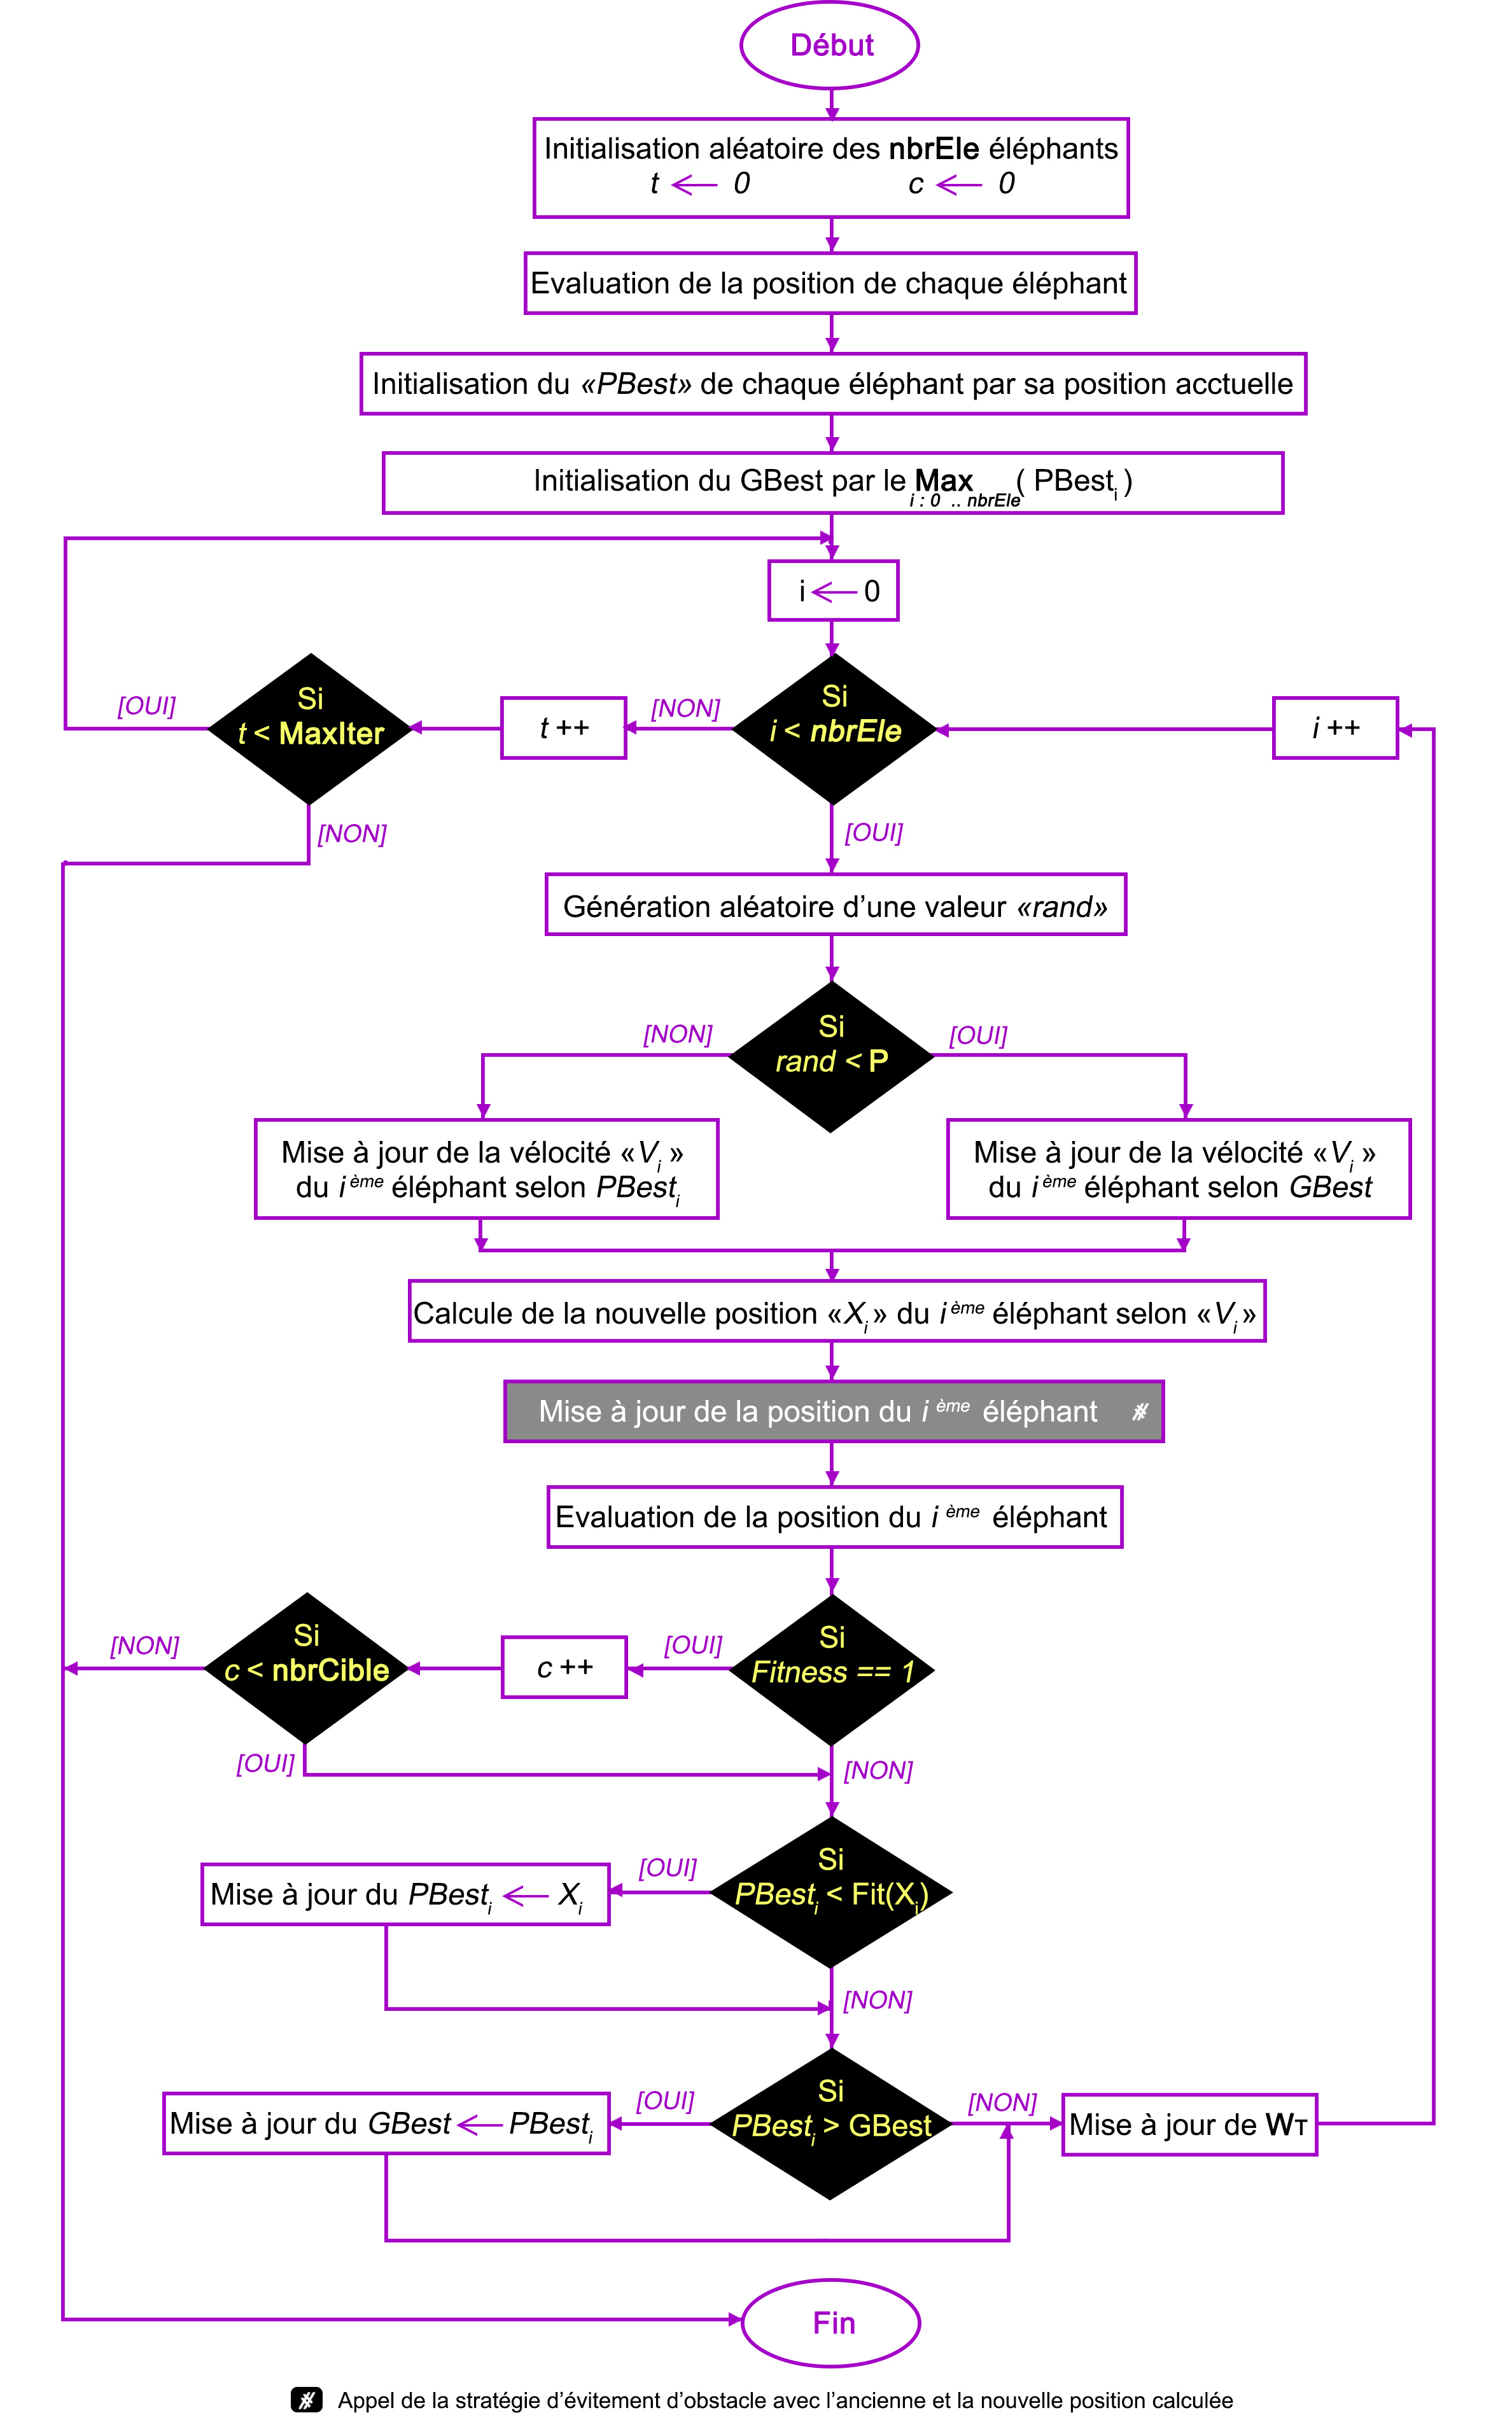
\includegraphics[width=0.8\textwidth]{eswsa.jpg}%
	\vspace{-0.3cm}
	\captionof{figure}{Organigramme du mode de fonctionnement de l'approche ESWSA.}\label{eswsa}%
\end{center}







\section{Conclusion}
Les deux algorithmes présentés reposent sur le comportement des éléphants, mais vus sous deux angles bien différents. C'est pourquoi leur fonctionnement n'a rien en commun, exploitant chacun un aspect différent relatif aux éléphants et groupes d'éléphants.
Le dernier chapitre sera consacré à la réalisation et expérimentations de toutes les approches citées dans ce chapitre et celui qui le précède.


\let\cleardoublepage\clearpage
% Chapter 4

\chapter{Chapitre 6 : Validation Expérimentale } % Main chapter title

\label{Chapter6} % For referencing the chapter elsewhere, use \ref{Chapter1} 

%----------------------------------------------------------------------------------------


\section{Introduction}
Les expérimentations sont essentielles pour la validation des algorithmes et approches en général. Cette étape nécessite de déterminer les caractéristiques des machines utilisées ainsi que la description de la partie logicielle dont nous avons eu besoin, mais surtout une organisation cohérente des tests expérimentaux réalisés. C'est justement l'objet de ce chapitre, dont la structure est décrite comme suit :\\
$-$ Description de l'environnement de développement.\\
$-$ Expérimentations relatives au paramétrage des approches de recherche.\\
$-$ Expérimentations sur les environnements, dont l'organisation est détaillée, suivies des résultats obtenus regroupés par types d'expérimentations et par types d'environnements.\\
$-$ Présentation du simulateur accompagné de son manuel d'utilisation.



\section{Environnement de développement}
\vspace{-0.2cm}
Comme pour toute expérimentation l'environnement de test est un élément clé pour la bonne interprétation des résultats obtenus.

\subsection{Matériel}
\vspace{-0.2cm}
Nous avons utilisé deux machines (Laptop) possédant les caractéristiques et capacités suivantes :


\noindent
\fbox{\parbox{\textwidth}{
		\begin{multicols}{2}
			\begin{minipage}[t]{0.45\textwidth}
				\underline{\textbf{Machine 1 :}}
				\vspace{0.2cm}
				\begin{description}
					\item[Mémoire RAM:] 8 Go
					\item[Processeur:] Intel® Core™ i5-6200U CPU  2.30GHz x 4 
					\item[Carte graphique:] Intel® HD Graphics 520 (Skylake GT2) x86/MMX/SSE2
					\item[Type de l'OS:] UBUNTU 14.04 LTS  32-bit
				\end{description}
			\end{minipage}\hfill
			
			\columnbreak
			\begin{minipage}[t]{0.45\textwidth}
				\underline{\textbf{Machine 2 : }}
				\begin{center}
					\begin{description}
						\item[Mémoire RAM:] 8 Go
						\item[Processeur:] Intel® Core™ i5-3317U  @ 1.70Hz  1.70GHz
						\item[Carte graphique:] Intel® HD Graphics 520 \hspace{5.5cm}  \textbf{        .}
						\item[Type de l'OS:] UBUNTU 18.04 LTS  64-bit
					\end{description}
					
				\end{center}
			\end{minipage}\hfill
			
		\end{multicols}
	}}
	
	\subsection{Logiciels}
	Le développement de nos algorithmes a été exclusivement fait sous système d'exploitation \textbf{Linux} (\textit{Ubuntu}), celui-ci muni des logiciels suivants:
	\vspace{-0.3cm}
	\paragraph{Intellij IDEA : }
	C'est un environnement de développement de logiciels informatiques orienté \textbf{Java}, supportant une large palette de plugins. C'est un des nombreux produits développés par la compagnie \textit{JetBrains}. Celle-ci nous a été mise à disposition via une licence étudiant.
	
	Nous l'avons utilisé pour le développement de notre solution de recherche de cibles.
	\vspace{-0.3cm}
	\paragraph{Java : }  C'est un langage orienté objet académique qui a fait ses preuves, très largement utilisé pour ses nombreux avantages dont on cite: la portabilité, large diversité des librairies, conséquente documentation, ...etc.

	Nous avons eu recours à une bibliothèque seulement, cela pour l'interface graphique en (\textbf{javaFx}) de notre simulateur en Java.
	
	\paragraph{jfoenix-8.0.8.jar} JFoenix\footnote{Lien : https://github.com/jfoenixadmin/JFoenix} est une librairie mettant à disposition des composantes java qui implémentent Google Material Design, elle est open source et dédiée aux applications java, spécialement les interfaces \textit{javaFx}. 
	
	\vspace{-0.3cm}
	\paragraph{PyCharm : }	C'est un environnement de développement de logiciels informatiques sous langage \textbf{Python}, aussi fournis par la compagnie \textit{JetBrain}, nous avons obtenu ce logiciel sous licence étudiant.
	Nous l'avons principalement utilisé pour exploiter les résultats des expérimentations pour les traiter et traduire en graphes plus significatifs.
	\vspace{-0.3cm}
	\paragraph{Python : } C'est un langage de programmation interprété assez récent. Il est de plus en plus utilisé en vue de sa simplicité et polyvalence.
	
	
	
	
	
	

	\section{Expérimentations relatives aux approches}
	\subsection{Paramétrage du mini-GA incrémental}
	Notre algorithme génétique possède quatre paramètres empiriques comme décrits dans le chapitre 3, nous avons procédé à une suite de tests afin de trouver les meilleures valeurs de ces paramètres, sans passer par un réglage de paramètres exhaustif. 
	Pour cela, nous avons fixé les bornes de chaque paramètre en prenant en compte la taille d'une solution (3D ou 4D).
	
	Les meilleurs paramètres obtenus se présentent comme suit :
	\begin{itemize}
		\item [$\bullet$] Taille de la population : 20
		\item [$\bullet$] Nombre d'itérations : 30
		\item [$\bullet$] Nombre de mutations : 2
		\item [$\bullet$] Point de croisement : aléatoire.
	\end{itemize}
	
	\subsection{Paramétrage des approches de recherche de cibles}
	Pour chaque taille d'environnement, portée des cibles, nombre de cibles nous avons paramétré nos méthodes (BSO, Multi-BSO, EHO, ESWSA) à l'aide de l'algorithme génétique (mini-GA incrémental), la moyenne des cinq meilleurs paramètres obtenus est calculée afin de former le meilleur paramétrage
	
	\subsubsection{Réglage de Paramètres de BSO}
	\paragraph{Flip : } Pour cette approche, nous avons constaté durant le réglage de ses paramètres que la variable \textit{Flip} influence grandement l'évolution de la recherche. Une valeur de \textit{Flip} trop grande empêche les abeilles d'explorer les zones distantes, de ce fait elle augmente les risques de stagnation, contrairement à des valeurs de \textit{Flip} trop petites qui favorisent l'exploration en dispersant trop les abeilles, ce qui peut mener à une recherche désorganisée.
	
	\paragraph{nbBees:} Le nombre d'abeilles \textit{"nbBees"} est un paramètre à double tranchant, car un grand nombre d'abeilles peut certes augmenter les chances de réussite, mais il amplifie considérablement le temps d'exécution.
	
	\paragraph{maxChances} pris avec une valeur trop grande cause une perte de temps et d'effort des abeilles, ce qui favorise une stagnation. En revanche, une valeur trop petite augmente les chances de passer à côté d'une solution intéressante. \\
	
	Les meilleurs paramètres obtenus pour l'algorithme BSO sont présentés dans le tableau suivant :
\begin{table}[h]
	\begin{tabular}{|l|p{0.3cm}|p{0.3cm}|p{0.3cm}|p{0.3cm}|p{0.3cm}|p{0.3cm}|p{0.5cm}|p{0.5cm}|p{0.6cm}|p{0.5cm}|p{0.5cm}|p{0.6cm}|p{0.3cm}|p{0.3cm}|p{0.3cm}|}
		\hline
		\multicolumn{1}{|c|}{\multirow{2}{*}{Type}} & \multicolumn{6}{c|}{Portée des cibles}                              & \multicolumn{6}{c|}{Taille d environnement}                         & \multicolumn{3}{l|}{\multirow{2}{*}{Nbr cibles}} \\ \cline{2-13}
		\multicolumn{1}{|c|}{}                                         & 
		\multicolumn{3}{c|}{mono-cible} & \multicolumn{3}{c|}{multi-cibles} & \multicolumn{3}{c|}{mono-cible} & \multicolumn{3}{c|}{multi-cibles} & \multicolumn{3}{l|}{}                                  \\ \hline
		\multicolumn{1}{|c|}{Paramètres}                               & 10       & 50       & 100       & 10        & 50        & 100       & 50       & 600      & 5000      & 50        & 600       & 5000      & 1                & 7                & 15               \\ \hline \hline
		Flip                                                           & 16       & 21       & 24        & 19        & 20        & 18        & 19       & 17       & 12        & 20        & 18        & 17        & 14               & 16               & 19               \\ \hline
		NbrBees                                                        & 15       & 14       & 11        & 9         & 12        & 13        & 11       & 16       & 21        & 10        & 12        & 23        & 14               & 17               & 20               \\ \hline
		MaxChances                                                     & 1        & 2        & 1         & 2         & 3         & 1         & 1        & 1        & 1         & 1         & 1         & 1         & 2                & 2                & 2                \\ \hline
	\end{tabular}
	\caption{Meilleurs paramètres pour BSO.}
\end{table}
	
	\vspace{-0.3cm}
	\subsubsection{Réglage de Paramètres de Multi-BSO}
	\paragraph{Flip :} Ce paramètre dans l'approche Multi-BSO ne doit pas être trop petit, car cela causerait une exploration trop grande et les abeilles se verront dispersées et perdraient leur organisation en groupes, d'autre part des valeurs exagérément grandes ralentiraient l'avancement de la recherche.
	
	
	
	\paragraph{nbSwarms \& nbBees \& MaxChances :} Cette méthode se distingue de la précédente par le nombre de groupes d'abeilles \textbf{nbSwarms}, dont les valeurs ont le même impacte que le nombre d'abeilles \textbf{nbBees} dans BSO.
	
	D'ailleurs le nombre d'abeilles \textbf{nbBees} par groupe et le paramètre \textbf{MaxChance} ont tous deux le même effet sur l'évolution de la recherche que sur BSO.\\
	
	\noindent
	Le tableau ci-dessous résume les meilleurs paramètres trouvés pour l'approche Multi-BSO :
	\vspace{-0.3cm}
	\begin{table}[h]
		\begin{tabular}{|l|p{0.3cm}|p{0.3cm}|p{0.3cm}|p{0.3cm}|p{0.3cm}|p{0.3cm}|p{0.5cm}|p{0.5cm}|p{0.6cm}|p{0.5cm}|p{0.5cm}|p{0.6cm}|p{0.35cm}|p{0.35cm}|p{0.35cm}|}
			\hline
			\multicolumn{1}{|c|}{\multirow{2}{*}{Type}} & \multicolumn{6}{c|}{Portée des cibles}                              & \multicolumn{6}{c|}{Taille d environnement}                         & \multicolumn{3}{l|}{\multirow{2}{*}{Nbr cibles}} \\ \cline{2-13}
			\multicolumn{1}{|c|}{}                      & \multicolumn{3}{c|}{mono-cible} & \multicolumn{3}{c|}{multi-cibles} & \multicolumn{3}{c|}{mono-cible} & \multicolumn{3}{c|}{multi-cibles} & \multicolumn{3}{l|}{}                                  \\ \hline
			\multicolumn{1}{|c|}{Paramètres}            & 10       & 50       & 100       & 10        & 50        & 100       & 50       & 600      & 5000      & 50        & 600       & 5000      & 1                & 7                & 15               \\ \hline  \hline
			Flip                                        & 20       & 21       & 18        & 21        & 20        & 30        & 15       & 23       & 42        & 20        & 25        & 40        & 20               & 20               & 22               \\ \hline
			NbrBees                                     & 4        & 4        & 4         & 4         & 4         & 3         & 3        & 3        & 5         & 3         & 4         & 5         & 3                & 4                & 4                \\ \hline
			MaxChances                                  & 2        & 2        & 1         & 3         & 2         & 1         & 1        & 1        & 1         & 1         & 1         & 2         & 2                & 1                & 2                \\ \hline
			NbSwarms                                    & 3        & 4        & 4         & 4         & 4         & 3         & 3        & 4        & 5         & 4         & 4         & 5         & 4                & 4                & 4                \\ \hline
		\end{tabular}
		\caption{Meilleurs paramètres pour Multi-BSO.}
	\end{table}
		
	\vspace{-0.3cm}
	\subsubsection{Réglage de Paramètres de EHO}
	
	\paragraph{nbClan \& nbEle}
	Le nombre de clans \textbf{nbClan} et d'éléphants par clan \textbf{nbEle} influencent directement les temps d'exécution et l'efficacité de la recherche, car des valeurs trop grandes (trop de clans et d'éléphants) augmentent les temps d'exécution, par contre leur affecter des valeurs trop petites réduit considérablement l'efficacité d'EHO.
	
	\paragraph{Alpha ($\alpha$)} D'une part, si le paramètre $\alpha$ prend des valeurs trop grandes, les éléphants convergeront vers des positions proches de la meilleure solution trop vite, cela engendrera leur stagnation dans un minimum local. D'autre part, une valeur trop petite ralentirait le processus de recherche en raison des déplacements très petits entre deux itérations consécutives.
	
	\paragraph{Beta ($\beta$)} Enfin, une valeur trop proche du 1 pour $\beta$ peut empêcher la convergence vers la solution optimale, car l'éléphant \textit{"matriarche"} sera retenu par le centre de gravité du clan qui n'est pas forcément dans la direction de la meilleure solution. Par contre, avec une valeur trop petite (proche du 0) l'éléphant se détachera de son clan, ce qui causera de grands écarts dans les déplacements.\\
	
	Les meilleurs paramètres de l'algorithme EHO sont donnés dans le tableau qui suit :
	\begin{table}[h]
		\begin{tabular}{|l|p{0.3cm}|p{0.3cm}|p{0.3cm}|p{0.3cm}|p{0.3cm}|p{0.3cm}|p{0.5cm}|p{0.5cm}|p{0.6cm}|p{0.5cm}|p{0.5cm}|p{0.6cm}|p{0.4cm}|p{0.4cm}|p{0.4cm}|}
			\hline
			\multicolumn{1}{|c|}{\multirow{2}{*}{Type}} & \multicolumn{6}{c|}{Portée des cibles}                              & \multicolumn{6}{c|}{Taille d environnement}                         & \multicolumn{3}{l|}{\multirow{2}{*}{Nbr cibles}} \\ \cline{2-13}
			\multicolumn{1}{|c|}{}                      & \multicolumn{3}{c|}{mono-cible} & \multicolumn{3}{c|}{multi-cibles} & \multicolumn{3}{c|}{mono-cible} & \multicolumn{3}{c|}{multi-cibles} & \multicolumn{3}{l|}{}                                  \\ \hline
			\multicolumn{1}{|c|}{Paramètres}            & 10        & 50       & 100      & 10         & 50        & 100      & 50        & 600      & 5000     & 50        & 600       & 5000      & 1                & 7                & 15               \\ \hline \hline
			nbrClan                                     & 3         & 3        & 2        & 4          & 4         & 4        & 3         & 4        & 4        & 4         & 4         & 5         & 3                & 4                & 4                \\ \hline
			nbrEle                                      & 3         & 3        & 3        & 3          & 3         & 3        & 3         & 3        & 4        & 3         & 4         & 4         & 3                & 3                & 4                \\ \hline
			alpha ($\alpha$)                            & 0.5       & 0.5      & 0.4      & 0.3        & 0.4       & 0.6      & 0.4       & 0.5      & 0.3      & 0.5       & 0.5       & 0.4       & 0.6              & 0.5              & 0.5              \\ \hline
			beta ($\beta$)                              & 0.3       & 0.4      & 0.3      & 0.4        & 0.3       & 0.5      & 0.5       & 0.4      & 0.6      & 0.5       & 0.5       & 0.4       & 0.4              & 0.4              & 0.5              \\ \hline
		\end{tabular}
		\caption{Meilleurs paramètres pour EHO.}
	\end{table}
	
	\vspace{-0.5cm}
	
	\subsubsection{Réglage de Paramètres de ESWSA}
	
	\paragraph{Nombre d’éléphants :} Comme on a pu le supposer, l'augmentation du nombre d'éléphants a tendance à accélérer la recherche en termes de nombre d'itérations, mais aboutir à des solutions en des temps plus élevés.
	
	
	\paragraph{Wt}:
	Nous avons remarqué que quand le nombre d'itérations \textit{t} augmente, la quantité du poids d'inertie \textit{$W^t$} diminue. Autrement dit plus les éléphants avancent (nombre d'itérations) plus l'influence de l'ancienne vélocité diminue, ce qui permet une meilleure exploration.
	
	\paragraph{Vélocité}:
	L'initialisation de la vélocité influe sur la dynamique de la recherche, une initialisation aléatoire non-nulle $V_{i}=(valx,valy)$ à de grandes valeurs  disperse les éléphants dans l'environnement. Contrairement à une initialisation nulle $V_{i}=(0,0)$ qui permet des déplacements à pas progressifs.    
	
	L'initialisation à valeurs aléatoires bornées moyennes a été la plus satisfaisante, ces valeurs privilégie l'exploration au début de la recherche.
	
	\paragraph{P}:
	Lors du paramétrage à l'aide du GA, nous avons remarqué que lorsque \textit{p} est très petit, chaque éléphant ne prend en considération que sa meilleure solution personnelle ($Pbest_i$) ce qui ralentit le processus de recherche de cibles. Les éléphants auront tendance à repasser par les mêmes chemins et parfois stagner dans un optimum local, comme le montre les figures %\ref{eswsa1}, 
	\ref{eswsa4}, \ref{eswsa8} et \ref{eswsa16} pour une valeur de $p=0$.
	

%		\begin{minipage}{.5\textwidth}
%			\centering
%			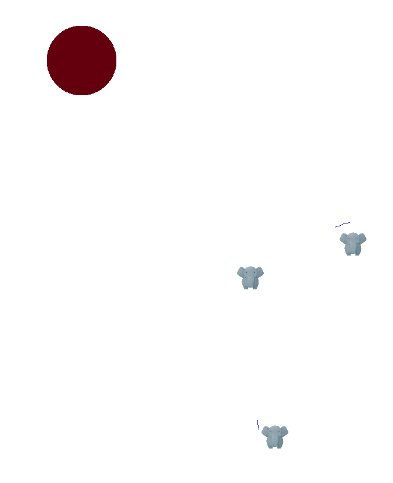
\includegraphics[scale=0.15]{eswsa1.png}
%			\captionof{figure}{ESWSA à l'itération 1}
%			\label{eswsa1}
%		\end{minipage}%

		\begin{minipage}{0.3\textwidth}
			\centering
			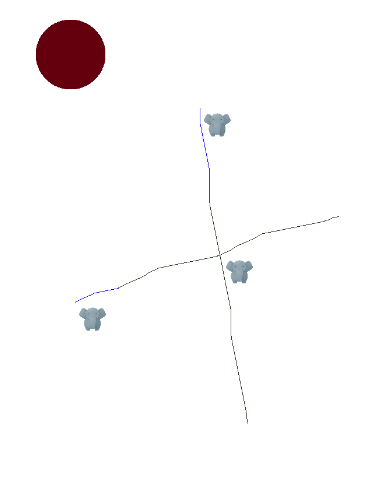
\includegraphics[width=0.9\textwidth]{eswsa4.png}
			\captionsetup{width=.9\linewidth}
			\captionof{figure}{ESWSA à l'itération 4}
			\label{eswsa4}
		\end{minipage}
		\hspace{0.2cm}
		\begin{minipage}{0.3\textwidth}
			\centering
			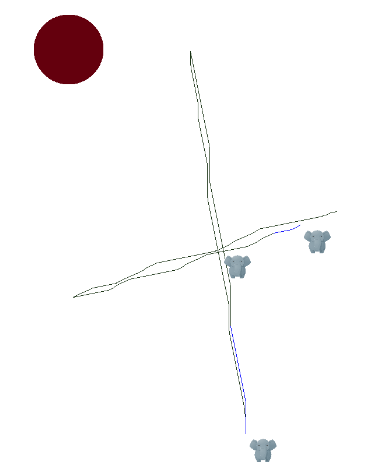
\includegraphics[width=0.9\textwidth]{eswsa8.png}
			\captionsetup{width=.9\linewidth}
			\captionof{figure}{ESWSA à l'itération 8}
			\label{eswsa8}
		\end{minipage}
		\hspace{0.2cm}
		\begin{minipage}{0.3\textwidth}
			\centering
			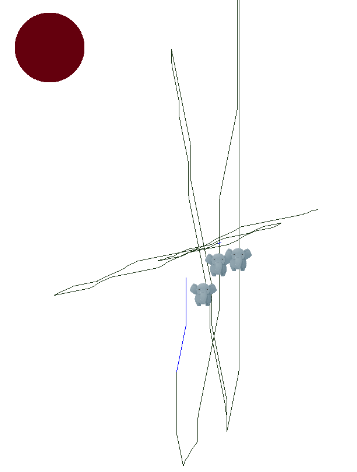
\includegraphics[width=0.89\textwidth]{eswsa16.png}
			\captionsetup{width=.9\linewidth}
			\captionof{figure}{ESWSA à l'itération 16}
			\label{eswsa16}
		\end{minipage}

	
	Par contre, une grande valeur de \textit{p} pousse les éléphants à suivre la même meilleure solution globale (\textit{Gbest}), convergeant ainsi vers une même cible ce qui cause un manque d'intensification.
	
	
	Le tableau suivant illustre les meilleurs paramètres obtenus pour l'algorithme ESWSA :
	\begin{table}[h]
		\begin{tabular}{|l|p{0.3cm}|p{0.3cm}|p{0.3cm}|p{0.3cm}|p{0.3cm}|p{0.3cm}|p{0.5cm}|p{0.5cm}|p{0.6cm}|p{0.5cm}|p{0.5cm}|p{0.6cm}|p{0.4cm}|p{0.4cm}|p{0.4cm}|}
			 \hline
			\multicolumn{1}{|c|}{\multirow{2}{*}{Type}} & \multicolumn{6}{c|}{Portée des cibles}                              & \multicolumn{6}{c|}{Taille d environnement}                         & \multicolumn{3}{l|}{\multirow{2}{*}{Nbr cibles}} \\ \cline{2-13}
			\multicolumn{1}{|c|}{}                      & \multicolumn{3}{c|}{mono-cible} & \multicolumn{3}{c|}{multi-cibles} & \multicolumn{3}{c|}{mono-cible} & \multicolumn{3}{c|}{multi-cibles} & \multicolumn{3}{l|}{}                            \\ \hline
			\multicolumn{1}{|c|}{Paramètres}            & 10        & 50       & 100      & 10         & 50        & 100      & 50        & 600      & 5000     & 50        & 600       & 5000      & 1              & 7              & 15             \\ \hline \hline
			nbrEle                                      & 16        & 15       & 10       & 19         & 17        & 14       & 12        & 14       & 19       & 16        & 16        & 18        & 17             & 15             & 20             \\ \hline
			Wt                                          & 0.4       & 0.5      & 0.4      & 0.4        & 0.5       & 0.3      & 0.6       & 0.5      & 0.5      & 0.6       & 0.5       & 0.5       & 0.5            & 0.4            & 0.5            \\ \hline
			p                                           & 0.6       & 0.5      & 0.3      & 0.5        & 0.5       & 0.5      & 0.5       & 0.5      & 0.3      & 0.6       & 0.5       & 0.5       & 0.5            & 0.5            & 0.5            \\ \hline
		\end{tabular}
		\caption{Meilleurs paramètres pour ESWSA.}
	\end{table}

	
	
%	\newpage
	
	%%%%%%%%%%%%%%%%%%%%%%%%%%%%%%%%%%%%%%%%%%%%%%%%%%%% %%%%%%%%%%%%%%%%%%%%%%%%%%%%%%%%%%%%%%%%%%%%%%%%%%%%
	%%%%%%%%%%%%%%%%%%%%%%%%%%%%%%%%%%%%%%%%%%%%%%%%%%%%
	\vspace{-0.5cm}
	
	\section{Expérimentations relatives à l'environnement}
	Nous avons sélectionné trois paramètres à expérimenter pour observer le comportement de nos approches de recherche basées essaims.
	Ces paramètres sont : \textit{la portée des cibles}, \textit{la taille de l'environnement} et \textit{le nombre de cibles recherchées}.
	
	Pour cela, nous avons réalisé ces expérimentations pour les trois types d'environnements précédemment explicités dans le chapitre 3, qui sont : \textbf{simples}, \textbf{avec obstacles} et \textbf{complexes}.
	
	

	

	
	\subsection{Organisation des types d'expérimentations}
	Pour une question de clarté, nous avons jugé nécessaire de décrire comment est organisé chaque type d'expérimentation avons de passer aux résultats obtenus.
	
	
	\subsubsection{Organisation des expérimentations par rapport à la portée des cibles}
	Pour les expérimentations relatives à l'influence de la portée des cibles sur le comportement de nos algorithmes de recherche, nous avons fixé la taille de l'environnement à 500 $\times$ 500 positions en faisant varier la portée d'un rayon de 10 positions à 100 positions avec un pas de 10.
	
	Ainsi comme le montre la figure \ref{orgPortee}, les tests de ce type proviennent des exécutions sur 40 environnements (4 par portée), ce qui fait 400 exécutions pour le mono-cible et 400 autres pour le multi-cibles, pour chaque méta-heuristique (après paramétrage).
	
	\begin{center}	 
		\captionsetup{width=1\linewidth} 
		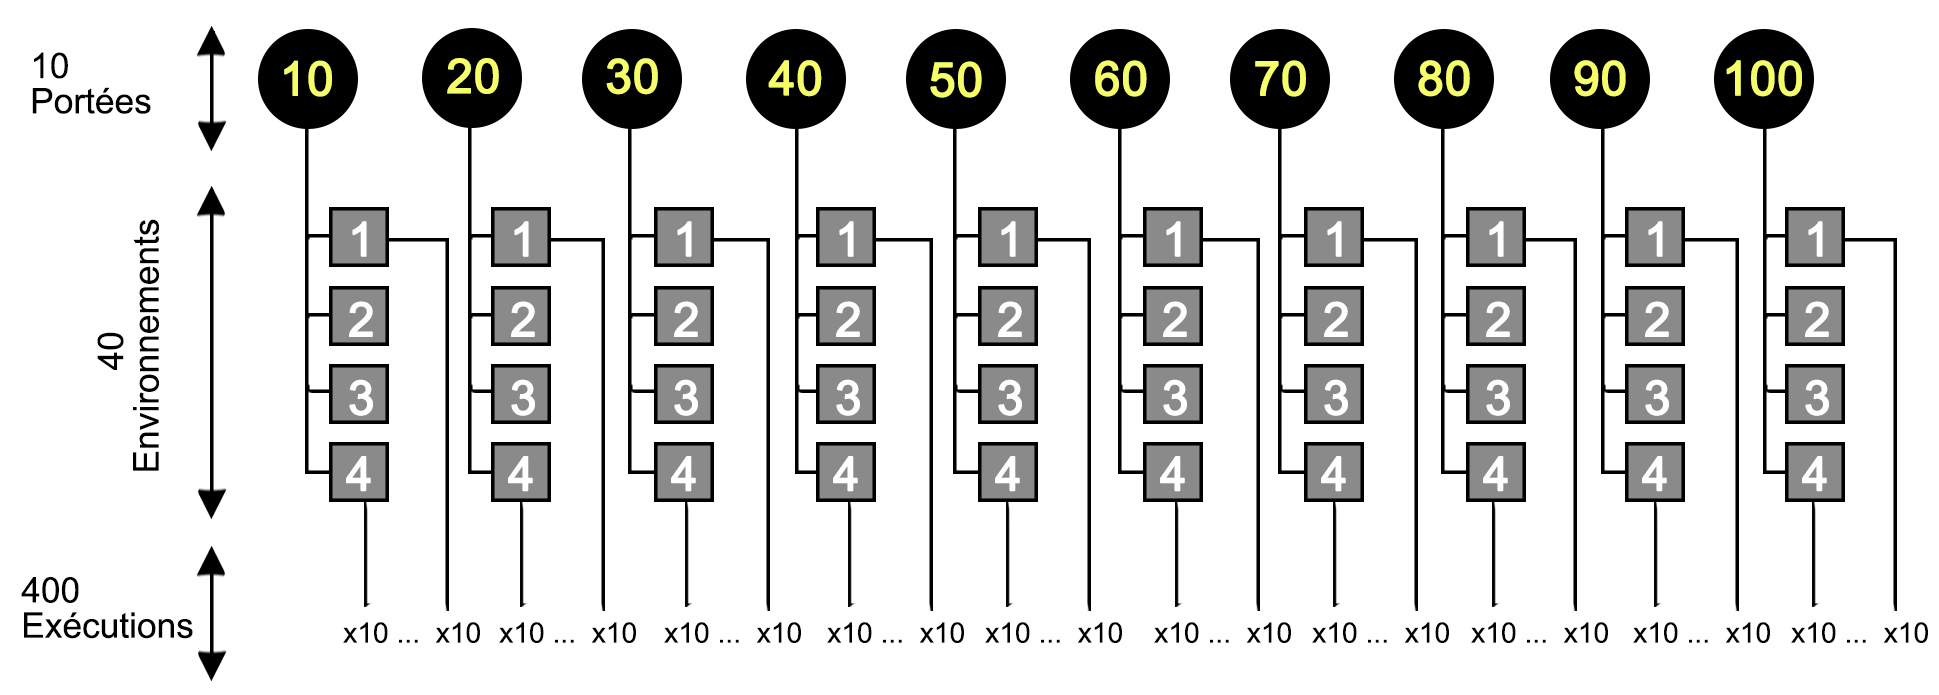
\includegraphics[width=0.7\textwidth]{org-portee.jpg}%
		\vspace{-0.1 cm}
		\captionof{figure}{Représentation de l'organisation des expérimentations sur la portée des cibles.}\label{orgPortee}%
	\end{center}
	
	\subsubsection{Organisation des expérimentations par rapport à la taille de l'environnement}
	Pour les expérimentations sur l'influence de la taille de l'environnement sur le comportement de nos méta-heuristiques à la recherche de cibles, nous avons adapté la portée des cibles à chaque taille d'environnement conformément à l'équation suivante :
	\begin{equation}
	portee = \frac{taille_{Cot\acute{e}} \times 10}{100} = \frac{taille_{Cot\acute{e}}}{10}
	\label{porteeEnv}
	\end{equation}	
	Ce qui revient à :
	\begin{equation}	
	S_{cible} = \frac{\sqrt{S_{env}}}{5} \times \pi
	\end{equation}
	
	Avec :
	\begin{itemize}
		\item[$-$] $taille_{Cot\acute{e}}$ : taille du coté de l'environnement carré.
		\item[$-$] $S_{cible}$ : surface d'émission de la cible (rayon = portée).
		\item[$-$] $S_{env}$ : surface de l'environnement de recherche ($S_{env}$ = $taille_{Cot\acute{e}}$).\\
	\end{itemize}
	
	Pour cela nous avons sélectionné dix différentes tailles d'environnement, les tailles du coté de ces environnements sont comme suit : 50, 100, 200, 400, 600, 800, 1000, 1500, 3000, 5000.
	
	Les surfaces respectives sont les suivantes: 2500, 10000, 40000, 160000, 360000, 640000, 1000000, 2250000, 9000000, 25000000.
	
	Les portées correspondantes sont: 5, 10, 20, 40, 60, 80, 100, 150, 300, 500.
	
	
	\textbf{ }\\
	Les résultats des tests liés à ce type d'expérimentation sont le résultat de 40 exécutions par taille d'environnement (4 configurations pour chaque taille), ce qui revient à un total de 400 exécutions pour le mono-cible et 400 autres pour le multi-cibles et ce pour chaque approche (après paramétrage). Le schéma \ref{orgSize} ci-dessous illustre cette organisation.
	
	\begin{center}	  
		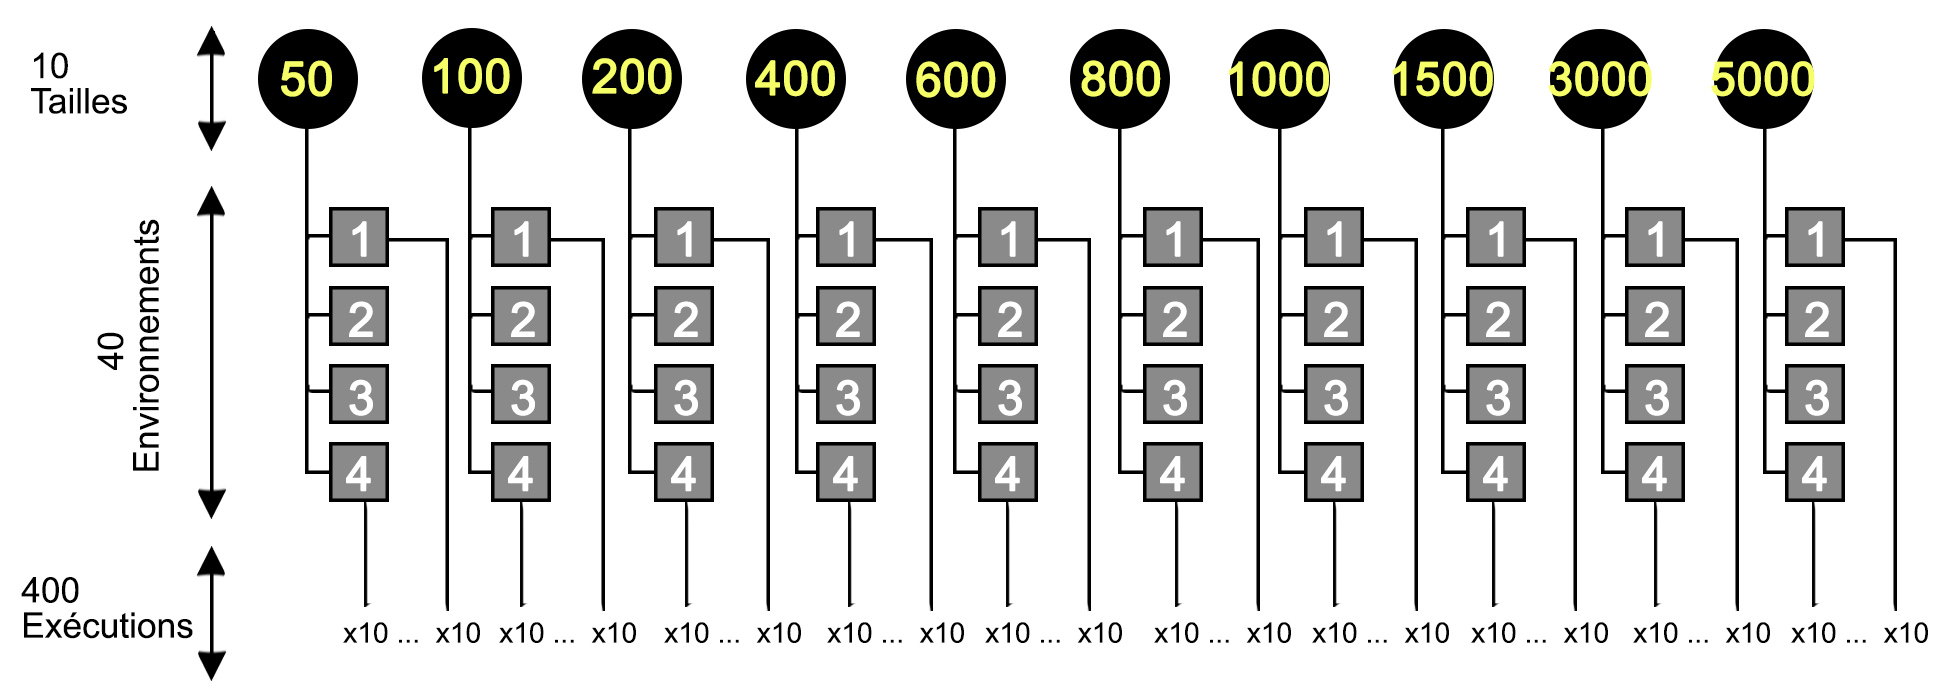
\includegraphics[width=0.75\textwidth]{org-size.jpg}%
		\vspace{-0.1 cm}
		\captionof{figure}{Représentation de l'organisation des expérimentations sur la taille des environnements.}\label{orgSize}%
	\end{center}
	
	\subsubsection{Organisation des expérimentations par rapport au nombre de cibles}
	Ces expérimentations permettent d'étudier l'impacte du changement du nombre de cibles présentes dans nos environnements sur le comportement de nos méta-heuristiques (BSO, EHO, ESWSA et Multi-BSO).
	Pour cela, nous avons fixé la taille des environnements à 500 $\times$ 500 positions ainsi qu'une portée de cible égale à 50 (Conformément à l'équation \ref{porteeEnv}).
	
	Nous avons pris le nombre de cibles compris entre 1 et 15 (bornes incluses) avec un pas de 2, ce qui nous donne les 8 nombres de cibles suivants : 1, 3, 5, 7, 9, 11, 13, 15.\\
	
	De ce fait, les résultats des tests sont le fruit d'exécutions sur 32 environnements (4 par nombre de cibles) , ce qui correspond à 320 exécutions pour chacune des approches développées (après paramétrage).\\
	La figure \ref{orgNbrT} ci-dessous schématise cette organisation :
	
	\begin{center}	  
		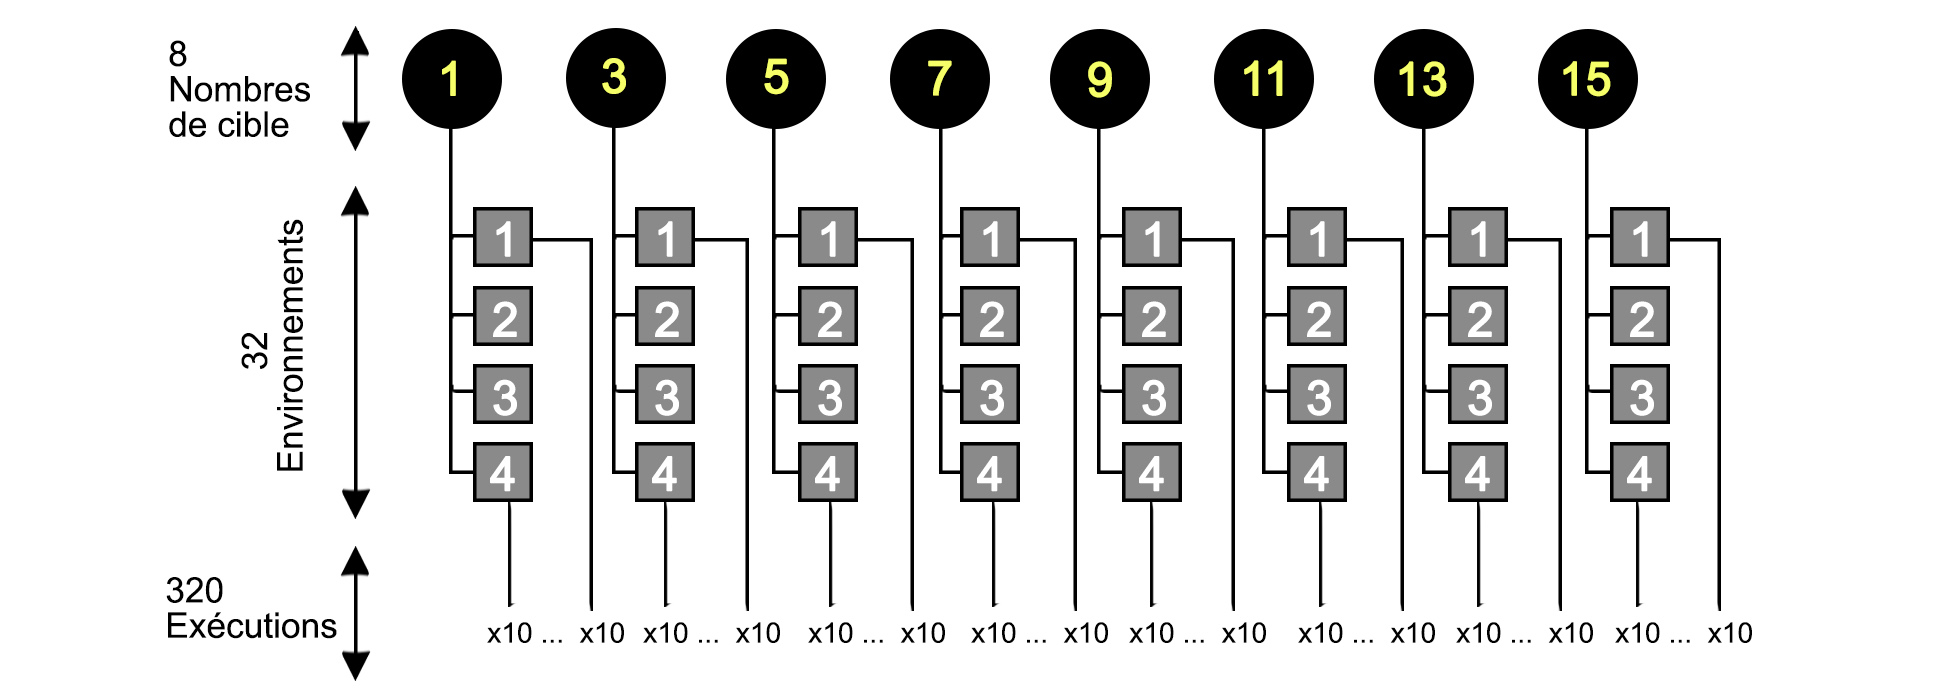
\includegraphics[width=0.8\textwidth]{org-nbrT.jpg}%
		\vspace{-0.1 cm}
		\captionof{figure}{Représentation de l'organisation des expérimentations sur le nombre de cibles.}\label{orgNbrT}%
	\end{center}
	
	
	

	%%%%%%%%%%%%%%%%%%%%%%%%%%%%%%%%%%%%%%%%%%%%%%%%%%%%%%
	%%%%%%%%%%%%%%%%%%%%%%%%%%%%%%%%%%%%%%%%%%%%%%%%%%%%%%\\
	%%%%%%%%%%%%%%%%%%%%%%%%%%%%%%%%%%%%%%%%%%%%%%%%%%%%%%\\
	
	
	\subsection{Expérimentations par rapport à la portée des cibles}
	
	\noindent
	\begin{minipage}[t]{0.5\textwidth}
		\subsubsection{Taux de réussite}
		
		La figure \ref{TP1} est un \textit{diagramme à bandes} représentant l'évolution du taux de réussite de chacune de nos méta-heuristiques par rapport aux différentes portées des cibles.\\
		
		Nous constatons que le taux de réussite est maximal (100\%) quelle que soit la valeur de la portée (de 10 à 100), autrement dit les algorithmes	implémentés arrivent toujours à trouver la ou les cible(s) sans atteindre le nombre maximal d'itérations qui est de 1000.
		
		Il est à noter que ces mêmes résultats ont été obtenus pour les trois types d'environnements (simple, avec obstacles et complexe) de dimensions 500 $\times$ 500 aussi bien dans les cas de mono-cible que de multi-cibles. 	
	\end{minipage}\hfill
	\begin{minipage}[t]{0.55\textwidth}
		\vspace{0.3cm}
		\captionsetup{width=0.8\linewidth}
		\centering\raisebox{\dimexpr \topskip-\height}{%
			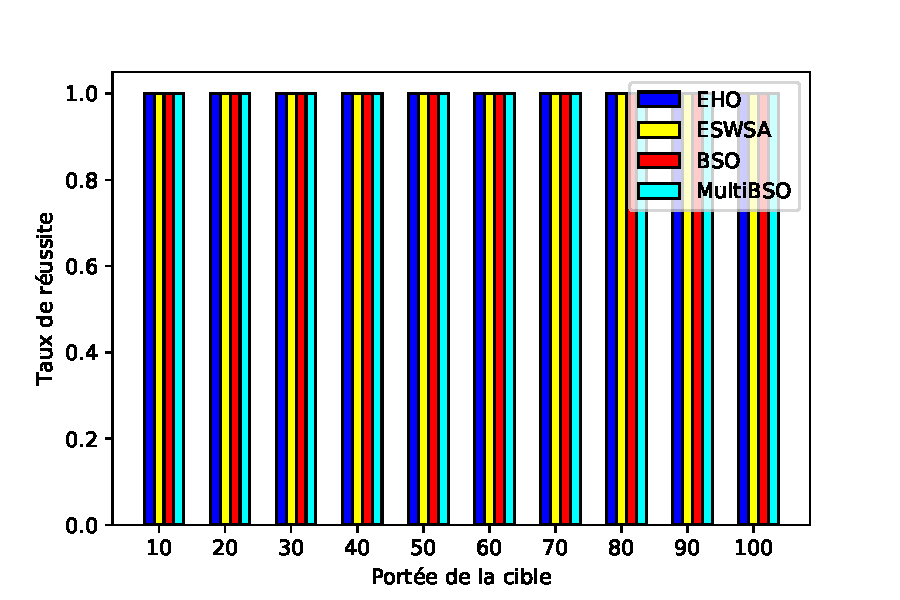
\includegraphics[width=\textwidth]{SansObs/BarChart/TauxPortee1.pdf}}
		\vspace{-0.3cm}
		\captionof{figure}{Comparaison de la variation du taux de réussite des algorithmes selon la portée des cibles.}
		\label{TP1}
	\end{minipage}\hfill
	
	
	\subsubsection{Variation du nombre d'itérations et temps d'exécution}
	\paragraph{a- Environnements simples (sans obstacles)}
	\paragraph{- Mono-cible}
	\vspace{-0.3cm}
	\textbf{ }\\
	Les figures \ref{IP1} et \ref{tP1} illustrent des \textit{diagrammes à lignes brisées}, représentant respectivement la variation du nombre d'itérations et temps d'exécution de chacune de nos approches confrontées aux différentes portées de la cible dans un environnement sans obstacle.\\
	\vspace{-0.2cm}
	
	On remarque que toutes les méthodes voient leur nombre d'itérations décroître avec l'élargissement de la portée de la cible. Pour les méthodes Multi-BSO, EHO et ESWSA, le nombre d'itérations est estimé entre 12 et 16 pour une portée égale à 10, puis décroît progressivement jusqu'à atteindre environ 2 ou 3 itérations pour la portée maximale. Quant à BSO, il débute avec un peu plus d'itérations (moyenne de 33), avant de diminuer pour rejoindre les autres méthodes lorsque la portée est maximale.\\
	\vspace{-0.2cm}
	
	Pour ce qui est des temps d'exécution, nos quatre méthodes s'exécutent en des temps records de moins de 0.08 secondes. BSO et Multi-BSO possèdent les meilleurs temps relativement stables et inférieurs à 0.02 secondes, suivies d'EHO atteignant les 0.05 secondes, enfin ESWSA est l'approche la plus lente en arrivant jusqu'à 0.08 secondes pour une portée égale à 100.
	
	\noindent
	\hspace{-0.5cm}
	\begin{minipage}[t]{0.55\textwidth}
		\captionsetup{width=0.8\linewidth}
		\centering\raisebox{\dimexpr \topskip-\height}{%
			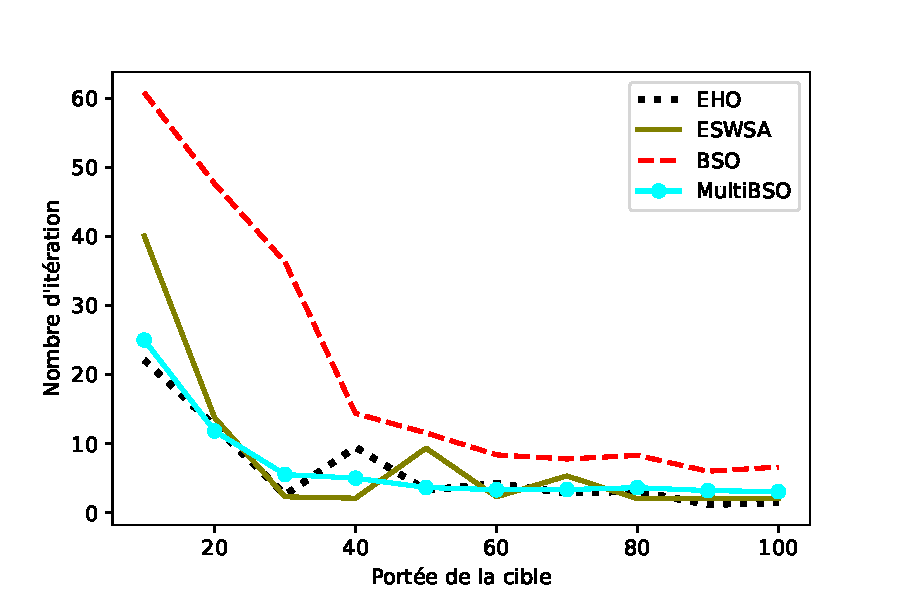
\includegraphics[width=\textwidth]{SansObs/LineChart/IterPortee1.pdf}}
		\captionof{figure}{Comparaison de la variation du nombre d'itérations des algorithmes selon la portée de la cible (sans obstacles).}
		\label{IP1}
	\end{minipage}\hfill
	\hspace{-0.5cm}
	\begin{minipage}[t]{0.55\textwidth}
		\captionsetup{width=0.8\linewidth}
		\centering\raisebox{\dimexpr \topskip-\height}{%
			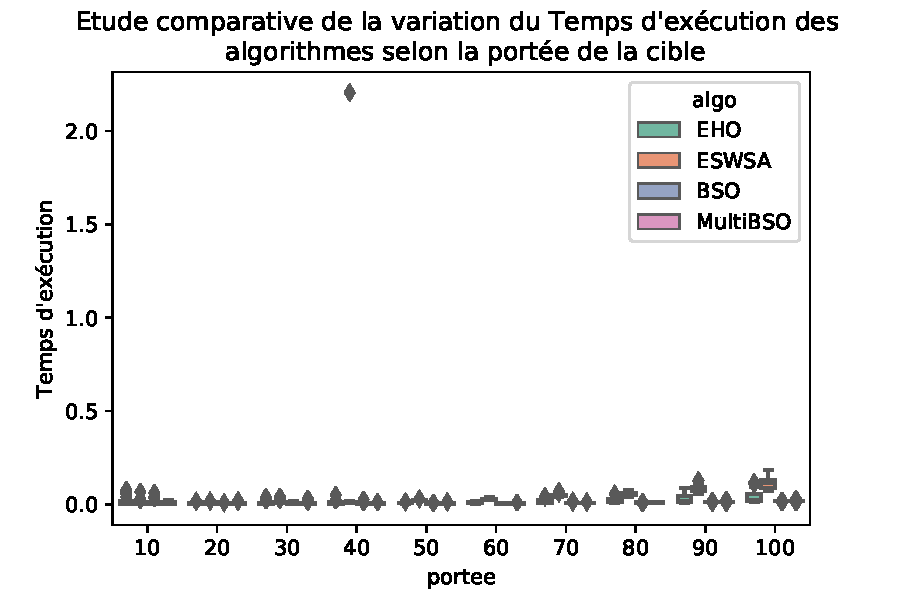
\includegraphics[width=\textwidth]{SansObs/LineChart/TimePortee1.pdf}}
		\captionof{figure}{Comparaison de la variation du temps d'exécution des algorithmes selon la portée de la cible (sans obstacles).}
		\label{tP1}
	\end{minipage}\hfill
	
	\paragraph{- Multi-cibles}
	\textbf{ }\\
	Les deux figures ci-dessous \ref{IP5} et \ref{tP5} sont représentatives de la variation du nombre d'itérations et temps d'exécution (dans cet ordre) de nos algorithmes, faces aux différentes portées des cibles dans des environnements sans obstacles.\\
	
	Nous distinguons trois comportements par rapport au nombre d'itérations, le premier est propre à BSO, celui-ci détient le plus grand nombre d'itérations pour toutes les portées, malgré la réduction de ce nombre de 107 à 29 en vue de l'augmentation des valeurs de la portée des cibles. 
	Compte au $2^{\grave{e}me}$, il est caractérisé par un nombre d'itérations avoisinant les 63 itérations pour une portée égale à 10, puis une diminution de ce nombre jusqu'à atteindre 8 à 4  itérations pour les cibles de portée 100; ce comportement concerne les deux méta-heuristiques EHO et ESWSA.
	Enfin, le $3^{\grave{e}me}$ comportement est celui de Multi-BSO, possédant le plus petit nombre d'itérations initial 31 qui diminue graduellement jusqu'à 9 itérations pour la portée égale à 100s.\\
	
	En termes de temps d'exécution, seul ESWSA subit une augmentation visible allant de 0.15 à 0.83 secondes pour les portées de 10 à 100 respectivement,  les trois autres algorithmes ne dépassent pas les 0.23 secondes, cette valeur correspondant aux résultats d'EHO pour la portée de 100 positions, BSO et Multi-BSO ayant des temps légèrement inférieurs.
	
	\noindent
	\hspace{-0.5cm}
	\begin{minipage}[t]{0.55\textwidth}
		\captionsetup{width=0.8\linewidth}
		\centering\raisebox{\dimexpr \topskip-\height}{%
			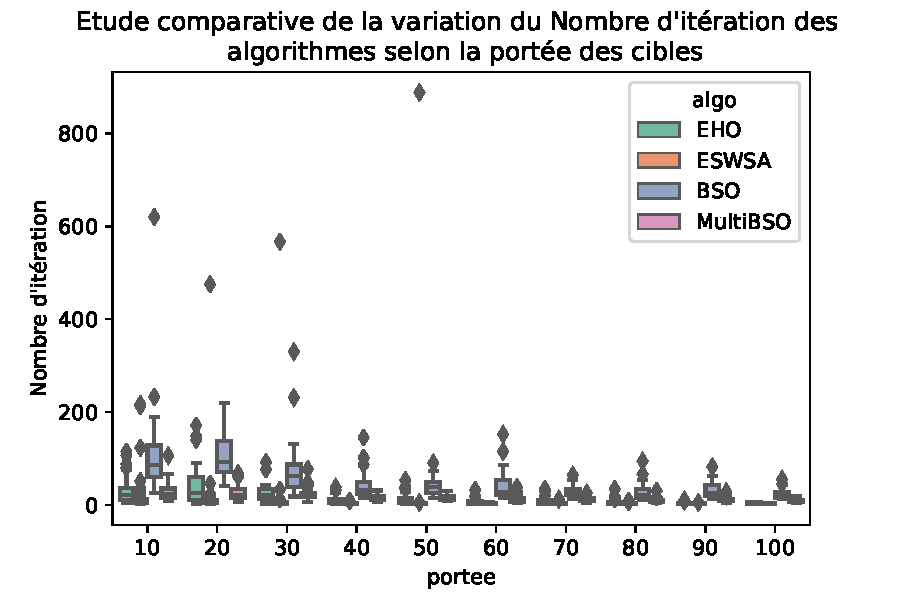
\includegraphics[width=\textwidth]{SansObs/LineChart/IterPortee5.pdf}}
		\captionof{figure}{Comparaison de la variation du nombre d'itérations des algorithmes selon la portée des cibles (sans obstacles).}
		\label{IP5}
	\end{minipage}\hfill
	\hspace{-0.5cm}
	\begin{minipage}[t]{0.55\textwidth}
		\captionsetup{width=0.8\linewidth}
		\centering\raisebox{\dimexpr \topskip-\height}{%
			\includegraphics[width=\textwidth]{SansObs/LineChart/TimePortee5.pdf}}
		\captionof{figure}{Comparaison de la variation du temps d'exécution des algorithmes selon la portée des cibles (sans obstacles).}
		\label{tP5}
	\end{minipage}\hfill
	
	
	\paragraph{b- Environnements avec obstacles}
	\paragraph{- Mono-cible}
	\textbf{ }\\
	Les deux \textit{diagrammes à lignes brisées} des figures \ref{IP1o} et \ref{tP1o} retracent la variation du nombre moyen d'itérations et temps moyens d'exécution de nos algorithmes faisant face à une portée croissante de la cible dans des environnements avec obstacles.\\
	\vspace{-0.2cm}
	
	Pour la première valeur de portée (égale à 10) l'approche BSO est celle qui nécessite le plus d'itérations (52.68), suivie d'EHO et Multi-BSO dont le nombre d'itérations est d'environ 14, enfin ESWSA, qui démarre avec seulement 3.58 itérations. 
	
	Pour toutes les méta-heuristiques, ce nombre évolue de manière inversement proportionnelle à la portée de la cible jusqu'à ce que la portée soit égale à 50 où il commence à se stabiliser autour de 9 itérations.\\
	\vspace{-0.2cm}
	
	Les temps d'exécution sont minorés par 0.001 secondes et majorés par la valeur 0.11 secondes, ce qui est remarquablement rapide. On distingue une augmentation des temps d'exécution pour ESWSA, plus légère pour EHO suite à l'élargissement de la surface de la portée de la cible. Les deux autres approches restent moyennement stables n'excédant pas les 0.02 secondes.   
	
	
	\vspace{-0.1cm}
	\noindent
	\hspace{-0.5cm}
	\begin{minipage}[t]{0.55\textwidth}
		\captionsetup{width=0.8\linewidth}
		\centering\raisebox{\dimexpr \topskip-\height}{%
			\includegraphics[width=\textwidth]{AvecObs/LineChart/IterPortee1.pdf}}
		\captionof{figure}{Comparaison de la variation du nombre d'itérations des algorithmes selon la portée de la cible (avec obstacles).}
		\label{IP1o}
	\end{minipage}\hfill
	\hspace{-0.5cm}
	\begin{minipage}[t]{0.55\textwidth}
		\captionsetup{width=0.8\linewidth}
		\centering\raisebox{\dimexpr \topskip-\height}{%
			\includegraphics[width=\textwidth]{AvecObs/LineChart/TimePortee1.pdf}}
		\captionof{figure}{Comparaison de la variation du temps d'exécution des algorithmes selon la portée de la cible (avec obstacles).}
		\label{tP1o}
	\end{minipage}\hfill
	
	
	\paragraph{- Multi-cibles}
	\textbf{ }\\
	Les figures \ref{IP5o} et \ref{tP5o} reflètent la variation du nombre d'itérations et temps d'exécution de nos quatre approches de recherche face aux portées des cibles, cela dans des environnements avec obstacles.\\
	
	Le nombre d'itérations diminue avec l'augmentation de la portée des cibles pour toutes les approches, néanmoins BSO se distingue par une diminution importante en passant d'une moyenne de 110.6 à 22.58 itérations. Contrairement à Multi-BSO, EHO et ESWSA qui varient entre 30 et 3 itérations.\\
	
	Pour ce qui est des temps d'exécution, nous remarquons que pour ESWSA la durée de recherche croît considérablement avec l'augmentation de la portée des cibles, comme nous pouvons le voir, il passe de 0.06 à 2.73 secondes. Les autres algorithmes qui se comportent de manière similaire, mais avec une marge moins importante passant de 0.01 à 0.23 secondes.
	
	
	\noindent
	\hspace{-0.5cm}
	\begin{minipage}[t]{0.55\textwidth}
		\captionsetup{width=0.8\linewidth}
		\centering\raisebox{\dimexpr \topskip-\height}{%
			\includegraphics[width=\textwidth]{AvecObs/LineChart/IterPortee5.pdf}}
		\captionof{figure}{Comparaison de la variation du nombre d'itérations des algorithmes selon la portée des cibles (avec obstacles).}
		\label{IP5o}
	\end{minipage}\hfill
	\hspace{-0.5cm}
	\begin{minipage}[t]{0.55\textwidth}
		\captionsetup{width=0.8\linewidth}
		\centering\raisebox{\dimexpr \topskip-\height}{%
			\includegraphics[width=\textwidth]{AvecObs/LineChart/TimePortee5.pdf}}
		\captionof{figure}{Comparaison de la variation du temps d'exécution des algorithmes selon la portée des cibles. (avec obstacles)}
		\label{tP5o}
	\end{minipage}\hfill
	
	
	\paragraph{c- Environnements complexes}
	\paragraph{- Mono-cible}
	\textbf{ }\\
	Les \textit{diagrammes à lignes brisées} des figures \ref{IP1c} et \ref{tP1c}, décrivent la variation du nombre d'itérations et temps d'exécution de nos approches, celles-ci confrontées aux diverses valeurs de portée de la cible recherchée et cela, dans des environnements complexes.\\
	
	Nous remarquons que le nombre d'itérations décroît avec l'augmentation de la portée de la cible, BSO débute avec le plus grand nombre de 60.83 pour en effectuer que 6.60 itérations lorsque la portée est à 100. ESWSA passe de 40.08 à 2.03 itérations. Quant à EHO, lui fluctue entre 22.13 et 1.48 itérations. Enfin Multi-BSO possède la courbe descendante la plus régulière qui passe de 25 à 3.05 itérations.\\
	
	Pour ce qui est des temps d'exécution, ceux de BSO, Multi-BSO ainsi qu'EHO connaissent une légère augmentation de 0.02 à 0.04 secondes contrairement à ceux d'ESWSA qui double passant de 0.06 à 0.12 secondes.
	
	
	
	\noindent
	\hspace{-0.5cm}
	\begin{minipage}[t]{0.55\textwidth}
		\captionsetup{width=0.8\linewidth}
		\centering\raisebox{\dimexpr \topskip-\height}{%
			\includegraphics[width=\textwidth]{Complex/LineChart/IterPortee1.pdf}}
		\captionof{figure}{Comparaison de la variation du nombre d'itérations des algorithmes selon la portée de la cible (complexe).}
		\label{IP1c}
	\end{minipage}\hfill
	\begin{minipage}[t]{0.55\textwidth}
		\centering\raisebox{\dimexpr \topskip-\height}{%
			\includegraphics[width=\textwidth]{Complex/LineChart/TimePortee1.pdf}}
		\captionof{figure}{Comparaison de la variation du temps d'exécution des algorithmes selon la portée de la cible (complexe).}
		\label{tP1c}
	\end{minipage}\hfill
	
	\paragraph{- Multi-cibles}
	\textbf{ }\\
	\'{A} travers les figures \ref{IP5c} et \ref{tP5c}, sont représentées respectivement la variation du nombre d'itérations et temps d'exécution de nos approches sous-mises aux dix valeurs de portée des cibles dans des environnements complexes.\\
	
	Comme dans le mode mono-cible, l'augmentation de la portée des cibles conduit à une baisse du nombre d'itérations. On note pour la méta-heuristique BSO une importante chute du nombre d'itérations allant de 110.6 à 22.58 suivie d'EHO et Multi-BSO qui se comportent de façon similaire avec un nombre d'itérations initial aux alentours de 80 qui dégringole aux environs de 8 itérations. Enfin, ESWSA possède la baisse la moins flagrante, passant de 46.88 à 3.08 itérations atteignant le nombre minimum d'itérations qui est de 3.\\
	
	Une hausse du taux de croissance est observée pour les temps d'exécution d'ESWSA (de 0.05 à 1.10 secondes). Contrairement à ceux de BSO, Multi-BSO et EHO où une stabilisation demeure avec une très légère augmentation pour EHO ne dépassant pas les 0.21 secondes, pour les portées entre 60 et 100.
	
	
	
	\noindent
	\hspace{-0.5cm}
	\begin{minipage}[t]{0.55\textwidth}
		\captionsetup{width=0.8\linewidth}
		\centering\raisebox{\dimexpr \topskip-\height}{%
			\includegraphics[width=\textwidth]{Complex/LineChart/IterPortee5.pdf}}
		\captionof{figure}{Comparaison de la variation du nombre d'itérations des algorithmes selon la portée des cibles (complexe).}
		\label{IP5c}
	\end{minipage}\hfill
	\hspace{-0.5cm}
	\begin{minipage}[t]{0.55\textwidth}
		\captionsetup{width=0.8\linewidth}
		\centering\raisebox{\dimexpr \topskip-\height}{%
			\includegraphics[width=\textwidth]{Complex/LineChart/TimePortee5.pdf}}
		\captionof{figure}{Comparaison de la variation du temps d'exécution des algorithmes selon la portée des cibles (complexe).}
		\label{tP5c}
	\end{minipage}\hfill
	
	
	\subsubsection{- Analyse relative à la portée des cibles}
	
	À travers les résultats commentés des cas du mono-cible et multi-cibles appliqués à toutes les approches, on peut retenir les points suivants :
	
	\begin{itemize}
		\item[$\bullet$] Même pour de petites portées des cibles, nos algorithmes arrivent à bout de la recherche avec succès.
		
		\item[$\bullet$] L'élargissement graduel de la portée des cibles a fait fléchir le nombre d'itérations.
		
		\item[$\bullet$] Malgré les temps d'exécution acceptables, ils sont moyennement plus importants pour le mode multi-cibles.
		
		\item[$\bullet$] La densité des obstacles influe la recherche, ce qui s'explique par l'augmentation des temps d'exécution et nombre d'itérations.\\
	\end{itemize}
	
	%%%%%%%%%%%%%%%%%%%%%%%%%%%%%%%%%%%%%%%%%%%%%%%%%%%%%%%%%%%%%%%%%%%%%%%%%%%%%%%%%%%%%%%%%%%%%%%%%%%%%%%%%%%%%%%%%%%%%%%%%%%%%%%%%%%%%%%%%%%%%%%%%%%%%%%%%%%%%%%%%%
	
	\subsection{Expérimentations par rapport à la taille de l'environnement}
	
	\subsubsection{Taux de réussite}
	\textbf{}
	
	\paragraph{a- Environnements simples (sans obstacles)}
	\textbf{}\\
	\noindent
	\begin{minipage}[t]{0.5\textwidth}
		\paragraph{- Mono-cible}
		\textbf{}\\
		Le graphe de la figure \ref{TS1} montre la variation du taux de réussite pour chaque approche développée, celles-ci sous-mises à diverses tailles d'environnements sans obstacles.\\
		
		Pour EHO et ESWSA, un taux maximal de réussite est observé quelle que soit la taille de l'environnement. En revanche, BSO et Multi-BSO voient leur taux de succès maximal diminuer jusqu'à 60\% pour BSO et 77\% pour Multi-BSO pour les deux dernières tailles c'est-à-dire 3000 et 5000.
		
		
		
	\end{minipage}\hfill
	\begin{minipage}[t]{0.55\textwidth}
		\captionsetup{width=0.8\linewidth}
		\centering\raisebox{\dimexpr \topskip-\height}{%
			\includegraphics[width=\textwidth]{SansObs/BarChart/TauxSize1.pdf}}
		\captionof{figure}{Comparaison de la variation du taux de réussite des algorithmes selon la taille de l'environnement (sans obstacles).}
		\label{TS1}
	\end{minipage}\hfill
	
	\textbf{ }
	
	\noindent
	\begin{minipage}[t]{0.5\textwidth}
		\paragraph{- Multi-cibles}
		\textbf{}\\
		La figure \ref{TS5} à droite décrit les taux de réussite dans la recherche des cibles, de chaque méta-heuristique en fonction de la variation de la taille des environnements sans obstacles.\\
		Nous nous apercevons que comme pour le mono-cible, EHO et ESWSA atteignent le taux de 100\% pour toutes les tailles, ce qui n'est pas le cas de BSO dont le taux de réussite décroît à partir de la $7^{\grave{e}me}$ taille d'environnement avec 99\% pour atteindre 51\% pour les environnements de taille 5000 et Multi-BSO dont les taux de succès des deux dernières tailles d'environnement sont respectivement de 85\% et 79\%.
		
	\end{minipage}\hfill
	\begin{minipage}[t]{0.55\textwidth}
		\captionsetup{width=0.8\linewidth}
		\centering\raisebox{\dimexpr \topskip-\height}{%
			\includegraphics[width=\textwidth]{SansObs/BarChart/TauxSize5.pdf}}
		\captionof{figure}{Comparaison de la variation du taux de réussite des algorithmes selon la taille de l'environnement (sans obstacles).}
		\label{TS5}
	\end{minipage}\hfill
	
	
	\paragraph{b- Environnements avec obstacles}
	\textbf{}\\
	\noindent
	\begin{minipage}[t]{0.5\textwidth}
		\paragraph{- Mono-cible}
		\textbf{}\\
		La figure \ref{TS1o} affiche la variation des taux de réussite de nos approches selon des tailles croissantes des environnements avec obstacles.\\
		
		Pour les tailles entre 50 et 1 500, tous nos algorithmes arrivent à obtenir les 100\% de taux de succès, toutefois les environnements de dimensions 3 000  connaissent une baisse de ce taux à 76\% pour BSO, mais toujours 100\% pour les autres. Enfin, pour les plus grands environnements Multi-BSO atteint un taux de 87\% contre 55\% pour BSO et 100\% pour EHO et ESWSA. 
		
		
		
	\end{minipage}\hfill
	\begin{minipage}[t]{0.55\textwidth}
		\captionsetup{width=0.8\linewidth}
		\centering\raisebox{\dimexpr \topskip-\height}{%
			\includegraphics[width=\textwidth]{AvecObs/BarChart/TauxSize1.pdf}}
		\captionof{figure}{Comparaison de la variation du taux de réussite des algorithmes selon la taille de l'environnement (avec obstacles).}
		\label{TS1o}
	\end{minipage}\hfill
	
	
	
	\noindent
	\begin{minipage}[t]{0.50\textwidth}
		\paragraph{- Multi-cibles}
		\textbf{}
		
		La figure \ref{TS5o} représente la variation des taux de succès de nos approches confrontées à plusieurs tailles d'environnement avec obstacles.\\
		
		EHO et ESWSA arrivent à maintenir les 100\% de taux de réussite pour toutes les tailles testées, contrairement à Multi-BSO qui relâche son taux de réussite à 83\% au bout de l'avant-dernière taille (3 000), et BSO qui déjà à partir des tailles 1 000 baisse à 67\% pour continuer à baisser jusqu'à 17\%. Toujours dans la limite du nombre d'itérations maximal (1 000).
		
	\end{minipage}\hfill
	\begin{minipage}[t]{0.55\textwidth}
		\captionsetup{width=0.8\linewidth}
		\centering\raisebox{\dimexpr \topskip-\height}{%
			\includegraphics[width=\textwidth]{AvecObs/BarChart/TauxSize5.pdf}}
		\captionof{figure}{Comparaison de la variation du taux de réussite des algorithmes selon la taille de l'environnement (avec obstacles).}
		\label{TS5o}
	\end{minipage}\hfill
	
	\textbf{ }
	\paragraph{c- Environnements complexes}
	\textbf{}\\
	\noindent
	\begin{minipage}[t]{0.5\textwidth}
		\paragraph{- Mono-cible}
		\textbf{}
		
		Dans la figure \ref{TS1c} est représentée la variation des taux de réussite de l'ensemble de nos approches exécutées sur différentes tailles d'environnements complexes.\\
		
		Pour toutes les tailles testées de 50 à 3 000 la totalité de nos algorithmes atteignent les 100\% de réussite, mais pour la dernière taille d'environnement (5 000) seuls EHO et ESWSA arrivent à garder le même taux de réussite, tels que Multi-BSO décent à 90\% et BSO chute à 60\%, car ils sont limités par le nombre d'itérations maximal.
		
	\end{minipage}\hfill
	\begin{minipage}[t]{0.55\textwidth}
		\captionsetup{width=0.8\linewidth}
		\centering\raisebox{\dimexpr \topskip-\height}{%
			\includegraphics[width=\textwidth]{SansObs/BarChart/TauxSize1.pdf}}
		\captionof{figure}{Comparaison de la variation du taux de réussite des algorithmes selon la taille de l'environnement (complexe).}
		\label{TS1c}
	\end{minipage}\hfill
	
	
	\noindent
	\begin{minipage}[t]{0.5\textwidth}
		\paragraph{- Multi-cibles}
		\textbf{}
		
		Les \textit{diagrammes à bandes} de la figure \ref{TS5c} décrivent comment les taux de succès de nos algorithmes varient faces aux tailles d'environnements complexes à la recherche de plusieurs cibles.\\
		
		EHO et ESWSA maintiennent les 100\% de taux de réussite pour toutes les tailles d'environnement, idem pour Multi-BSO sauf pour ce qui est de la dernière taille, il n'arrive qu'à 71\%. Par contre BSO décent sous la barre des 100\% dès la taille 1000, à partir de là, son taux fluctue entre 36\% et 98\% car freiné par le nombre d'itérations maximal.
		
	\end{minipage}\hfill
	\begin{minipage}[t]{0.55\textwidth}
		%\vspace{0.2cm}
		\captionsetup{width=0.8\linewidth}
		\centering\raisebox{\dimexpr \topskip-\height}{%
			\includegraphics[width=\textwidth]{Complex/BarChart/TauxSize5.pdf}}
		\captionof{figure}{Comparaison de la variation du taux de réussite des algorithmes selon la taille de l'environnement (complexe).}
		\label{TS5c}
	\end{minipage}\hfill
	
	
	
	\subsubsection{Variation du nombre d'itérations et temps d'exécution}
	\paragraph{a- Environnements simples (sans obstacles)}
	\textbf{}
	\vspace{-0.3cm}
	\noindent
	\paragraph{- Mono-cible}
	\textbf{ }
	
	Dans les figures \ref{IS1} et \ref{tS1} sont représentés la variation du nombre d'itérations et du temps d'exécution de nos méta-heuristiques pour l'ensemble des tailles d'environnement sans obstacles sélectionnées.\\
	\vspace{-0.2cm}
	
	Les méta-heuristiques inspirées des éléphants détiennent le nombre d'itérations le plus réduit, celui-ci varie entre 1 et 10 itérations pour EHO et entre 2 et 13 itérations pour ESWSA. Par contre, les deux variantes de BSO connaissent une importante augmentation du nombre d'itérations de 4 à 574 itérations pour BSO et de 2 à 189 pour Multi-BSO, suite à l'augmentation de la taille des environnements.\\
	\vspace{-0.2cm}
	
	Pour ce qui est de l'aspect "temps", toutes les approches sont sujettes à une croissance proportionnelle à la croissance des tailles d'environnement à différents coefficients près, tels que nous pouvons les ordonner selon la vitesse d'augmentation des temps d'exécution de l'algorithme le plus lent au plus rapide comme suit : ESWSA puis BSO suivis de Multi-BSO et enfin EHO, ce dernier atteint un maximum de 4.6 secondes pour une taille = 5 000.
	
	\noindent
	\hspace{-0.5cm}
	\begin{minipage}[t]{0.55\textwidth}
		\captionsetup{width=0.8\linewidth}
		\centering\raisebox{\dimexpr \topskip-\height}{%
			\includegraphics[width=\textwidth]{SansObs/LineChart/IterSIze1.pdf}}
		\captionof{figure}{Comparaison de la variation du nombre d'itérations des algorithmes selon la taille de l'environnement (sans obstacles).}
		\label{IS1}
	\end{minipage}\hfill
	\hspace{-0.5cm}
	\begin{minipage}[t]{0.55\textwidth}
		\captionsetup{width=0.8\linewidth}
		\centering\raisebox{\dimexpr \topskip-\height}{%
			\includegraphics[width=\textwidth]{SansObs/LineChart/TimeSIze1.pdf}}
		\captionof{figure}{Comparaison de la variation du temps d'exécution des algorithmes selon la taille de l'environnement (sans obstacles).}
		\label{tS1}
	\end{minipage}\hfill
	
	
	\noindent
	\paragraph{- Multi-cibles}
	\textbf{ }
	
	Les courbes des figures \ref{IS5} et \ref{tS5} illustrent la variation du nombre moyen d'itérations et temps moyens d'exécution de nos algorithmes vis-à-vis des différentes tailles d'environnement sans obstacles.\\
	\vspace{-0.2cm}
	
	Ici aussi, pour le mode multi-cibles EHO et ESWSA effectuent le moins d'itérations, avec une légère augmentation allant de 2.43 jusqu'à 19.43 itérations pour EHO, de 3.73 à 6.95 itérations pour ESWSA, cela pour l'agrandissement de la taille des environnements.
	Par ailleurs, BSO et Multi-BSO subissent une conséquente élévation du nombre d'itérations allant de 9.88 à 991.18 itérations pour BSO et de 5.95 à 865.53 pour ce qui est de Multi-BSO.\\
	\vspace{-0.2cm}
	
	Quant aux temps d'exécution, globalement nous pouvons dire que les temps d'exécution des algorithmes croient avec l'augmentation de la taille des environnements à différentes vitesses, tels que BSO passe progressivement de 0.001 à 6.57 secondes suivi de Multi-BSO avec des temps haussant de 0.001 à 11.75 secondes, puis EHO qui démarre à 0.001 pour atteindre les 19.43 secondes et enfin ESWSA qui enregistre les plus grands temps passant de  0.001 à 17.01 secondes.
	
	
	
	\noindent
	\begin{minipage}[t]{0.55\textwidth}
		\hspace{-0.5cm}
		\captionsetup{width=0.8\linewidth}
		\centering\raisebox{\dimexpr \topskip-\height}{%
			\includegraphics[width=\textwidth]{SansObs/LineChart/IterSIze5.pdf}}
		\captionof{figure}{Comparaison de la variation du nombre d'itérations des algorithmes selon la taille de l'environnement (sans obstacles).}
		\label{IS5}
	\end{minipage}\hfill
	\hspace{-0.5cm}
	\begin{minipage}[t]{0.55\textwidth}
		\captionsetup{width=0.8\linewidth}
		\centering\raisebox{\dimexpr \topskip-\height}{%
			\includegraphics[width=\textwidth]{SansObs/LineChart/TimeSIze5.pdf}}
		\captionof{figure}{Comparaison de la variation du temps d'exécution des algorithmes selon la taille de l'environnement (sans obstacles).}
		\label{tS5}
	\end{minipage}\hfill
	
	\paragraph{b- Environnements avec obstacles}
	\textbf{}
	\noindent
	\paragraph{- Mono-cible}
	\textbf{ }
	
	Les \textit{diagrammes à lignes brisées} des figures \ref{IS1o} et \ref{tS1o} font apparaître la variation du nombre d'itérations et temps d'exécution de BSO, Multi-BSO, EHO ainsi qu'ESWSA par rapport aux tailles des environnements avec obstacles.\\
	\vspace{-0.2cm}
	
	La figure de gauche montre que BSO détient le plus grand nombre d'itérations pour l'ensemble des tailles d'environnement, avec une augmentation allant de 2.55 à 566.18 itérations. Multi-BSO vient juste après avec des nombres d'itérations croissants tout en restant réduit jusqu'aux environnements de 3000 $\times$ 3000 où il arrive à 48.45 itérations qui par la suite grimpe vers 295.58 itérations pour les plus grands environnements.
	Enfin, EHO et ESWSA disposent des nombres d'itérations les plus réduis, fluctuant entre 1.08 et 29.78 itérations.\\
	\vspace{-0.2cm}
	
	Quant à la figure de droite, nous y discernons deux comportements tous deux croissants avec l'élargissement des surfaces des environnements, le $1^{er}$ englobe BSO, Multi-BSO et EHO qui possèdent des temps d'exécution minimes (entre 0.001 et 3.83 secondes), et le $2^{\grave{e}me}$ comportement concerne ESWSA avec des temps moyens plus ou moins élevés, allant de 0.001 à 15.56 secondes.
	
	
	
	\noindent
	\hspace{-0.3cm}
	\begin{minipage}[t]{0.55\textwidth}
		\captionsetup{width=0.8\linewidth}
		\centering\raisebox{\dimexpr \topskip-\height}{%
			\includegraphics[width=\textwidth]{AvecObs/LineChart/IterSIze1.pdf}}
		\captionof{figure}{Comparaison de la variation du nombre d'itérations des algorithmes selon la taille de l'environnement (avec obstacles).}
		\label{IS1o}
	\end{minipage}\hfill
	\hspace{-0.5cm}
	\begin{minipage}[t]{0.55\textwidth}
		\captionsetup{width=0.8\linewidth}
		\centering\raisebox{\dimexpr \topskip-\height}{%
			\includegraphics[width=\textwidth]{AvecObs/LineChart/TimeSIze1.pdf}}
		\captionof{figure}{Comparaison de la variation du temps d'exécution des algorithmes selon la taille de l'environnement (avec obstacles).}
		\label{tS1o}
	\end{minipage}\hfill
	
	\noindent
	\paragraph{- Multi-cibles}
	\textbf{ }
	
	Les figures \ref{IS5o} et \ref{tS5o} présentées ci-dessous, retracent la variation du nombre d'itérations et temps d'exécution de nos algorithmes testés sur plusieurs tailles d'environnement avec obstacles à la recherche de plusieurs cibles.\\
	\vspace{-0.2cm}
	
	BSO et Multi-BSO se distinguent avec des nombres élevés d'itérations, BSO débutant de 9.50 itérations et arrivant à la limite maximale de 1000 itérations, quant à Multi-BSO il passe d'une moyenne de 5.40 à 920.68 itérations. D'autre part EHO et ESWSA possèdent le moins d'itérations (entre 2.45 et 22.18 itérations).\\
	\vspace{-0.2cm}	
	
	Côté temps d'exécution, nous pouvons ordonner nos méthodes de la plus rapide à la plus long comme suit : BSO avec de 0.001 à 1.99 secondes suivie de Multi-BSO avec de 0.01 à 5.67 secondes puis EHO avec des temps entre 2.45 et 20.50 secondes, pour finir ESWSA dont les temps croissent de manière spectaculaire de 0.001 à 94.55 secondes. 
	
	
	
	\noindent
	\hspace{-0.5cm}
	\begin{minipage}[t]{0.55\textwidth}
		\captionsetup{width=0.8\linewidth}
		\centering\raisebox{\dimexpr \topskip-\height}{%
			\includegraphics[width=\textwidth]{AvecObs/LineChart/IterSIze5.pdf}}
		\captionof{figure}{Comparaison de la variation du nombre d'itérations des algorithmes selon la taille de l'environnement (avec obstacles).}
		\label{IS5o}
	\end{minipage}\hfill
	\hspace{-0.5cm}
	\begin{minipage}[t]{0.55\textwidth}
		\captionsetup{width=0.8\linewidth}
		\centering\raisebox{\dimexpr \topskip-\height}{%
			\includegraphics[width=\textwidth]{AvecObs/LineChart/TimeSIze5.pdf}}
		\captionof{figure}{Comparaison de la variation du temps d'exécution des algorithmes selon la taille de l'environnement (avec obstacles).}
		\label{tS5o}
	\end{minipage}\hfill
	
	
	
	\paragraph{c- Environnements complexes}
	\textbf{}
	\noindent
	\paragraph{- Mono-cible}
	\textbf{ }\\
	Dans les figures \ref{IS1c} et \ref{tS1c} sont décrites la variation du nombre d'itérations et celle du temps d'exécution de nos algorithmes selon la taille des environnements complexes.\\
	\vspace{-0.2cm}
	
	Nous pouvons regrouper les méta-heuristiques en deux groupes d'après l'évolution de leur nombre d'itérations, le $1^{er}$ groupe est constitué de BSO et Multi-BSO qui subit une importante croissance de ce nombre passant de 2.7 à 747.78 itérations pour BSO et de 2.05 à 444.45 itérations pour Multi-BSO.
	
	Le $2^{\grave{e}me}$ groupe est celui d'EHO et ESWSA, ceux-ci croient de manière bien plus raisonnable, soient de 1.35 à 13.83 itérations pour EHO et de 1.05 à 70.45 itérations pour ESWSA.\\
	\vspace{-0.2cm}
	
	Toutes nos approches connaissent un 
	accroissement des temps d'exécution avec l'élargissement des tailles d'environnement. ESWSA est celle dont les temps ont le plus augmenté (de 0.001 à 12.32 secondes), suivie d'EHO avec des temps qui passent de 0.001 à 3.03 secondes, puis vient Multi-BSO avec entre 0.001 et 1.92 secondes. Enfin, la plus rapide est BSO, dont les temps sont entre 0.001 et 1 seconde.
	
	
	
	\noindent
	\hspace{-0.5cm}
	\begin{minipage}[t]{0.55\textwidth}
		\captionsetup{width=0.8\linewidth}
		\centering\raisebox{\dimexpr \topskip-\height}{%
			\includegraphics[width=\textwidth]{Complex/LineChart/IterSIze1.pdf}}
		\captionof{figure}{Comparaison de la variation du nombre d'itérations des algorithmes selon la taille de l'environnement (complexe).}
		\label{IS1c}
	\end{minipage}\hfill
	\begin{minipage}[t]{0.55\textwidth}
		\captionsetup{width=0.8\linewidth}
		\centering\raisebox{\dimexpr \topskip-\height}{%
			\includegraphics[width=\textwidth]{Complex/LineChart/TimeSIze1.pdf}}
		\captionof{figure}{Comparaison de la variation du temps d'exécution des algorithmes selon la taille de l'environnement (complexe).}
		\label{tS1c}
	\end{minipage}\hfill
	
	
	\noindent
	\paragraph{- Multi-cibles}
	\textbf{ }\\
	\vspace{-0.2cm}
	
	Les courbes des figures \ref{IS5c} et \ref{tS5c} illustrent la variation du nombre moyen d'itérations et temps moyen d'exécution de nos algorithmes vis-à-vis des différentes tailles d'environnement complexes.\\
	\vspace{-0.2cm}
	
	Du point de vue du nombre d'itérations, ils commencent tous avec environ 3 à 12 itérations pour le plus petit environnement puis augmentent. Ici aussi, c'est BSO et Multi-BSO qui enregistrent les plus grands nombres avec un maximum de 1000 et 865.5 itérations respectivement, ensuite EHO va jusqu'à 29.3 itérations et enfin ESWSA ne dépasse pas la moyenne de 13.65 itérations.\\
	\vspace{-0.2cm}
	
	Quant aux temps d'exécution les 4 approches évoluent de la même manière que pour le mode mono-cible, mais avec tes temps plus importants, allant de 0.001 à 93.31 secondes pour ESWSA, grimpant de 0.001 à 15.55 secondes pour EHO, puis de 0.001 à 10.23 secondes pour Multi-BSO, enfin pour BSO les temps vont de 0.001 à 4.79 secondes.
	
	
	
	\noindent	
	\hspace{-0.5cm}
	\begin{minipage}[t]{0.55\textwidth}
		\captionsetup{width=0.8\linewidth}
		\centering\raisebox{\dimexpr \topskip-\height}{%
			\includegraphics[width=\textwidth]{Complex/LineChart/IterSIze5.pdf}}
		\vspace{-0.3cm}
		\captionof{figure}{Comparaison de la variation du nombre d'itérations des algorithmes selon la taille de l'environnement (complexe).}
		\label{IS5c}
	\end{minipage}\hfill
	\begin{minipage}[t]{0.55\textwidth}
		\captionsetup{width=0.8\linewidth}
		\centering\raisebox{\dimexpr \topskip-\height}{%
			\includegraphics[width=\textwidth]{Complex/LineChart/TimeSIze5.pdf}}
		\vspace{-0.3cm}
		\captionof{figure}{Comparaison de la variation du temps d'exécution des algorithmes selon la taille de l'environnement (complexe).}
		\label{tS5c}
	\end{minipage}\hfill
	
	\subsubsection{- Analyse relative à la taille des environnements}
	Suite aux résultats concernant la taille des environnements simples, avec obstacles et complexes selon les deux modes mono et multi-cibles, nous pouvons noter que :
	\begin{itemize}
		\item[$\bullet$] Contrairement aux deux approches inspirées des abeilles (BSO et Multi-BSO), les deux autres méta-heuristiques à savoir : EHO et ESWSA atteignent le taux maximum de réussite dans leur recherche de la ou les cible(s) quelle que soit la taille de l'environnement à explorer.
		\item[$\bullet$] Pour tous les algorithmes le nombre d'itérations croît avec l'augmentation de la taille des environnements, mais à des vitesses différentes. Telles qu'EHO et ESWSA effectuent le moins d'itérations.
		\item[$\bullet$] Les temps restent relativement acceptables pour le mono-cible, par-contre pour le mode multi-cible ils atteignent les 1min 30. C'est ESWSA le plus long.
		
		\item[$\bullet$] EHO et ESWSA minimisent le nombre d'itérations en raison des grands pas entre deux positions successives qu'ils génèrent, mais cela leur coûte cher en temps, ce qui est l'inverse de BSO et Multi-BSO qui effectuent de petits pas dans des temps moindres.
		
		\item[$\bullet$] Pour les deux modes et pour toutes les approches, les temps d'exécution et nombre d'itérations croissent avec l'augmentation de la complexité des environnements.
	\end{itemize}
	
	
	%%%%%%%%%%%%%%%%%%%%%%%%%%%%%%%%%%%%%%%%%%%%%%%%%%%%%%%%%%%%%%%%%%%%%%%%%%%%%%%%%%%%%%%%%%%%%%%%%%%%%%%%%%%%%%%%%%%%%%%%%%%%%%%%%%%%%%%%%%%%%%%%%%%%%%%%%%%%%%%%%%%%%
	
	
	
	\subsection{Expérimentations par rapport au nombre de cibles}
	
	\noindent
	\begin{minipage}[t]{0.55\textwidth}
		\subsubsection{Taux de réussite}
		Les taux de réussite sont présentés sous forme de \textit{diagramme à bandes} dans la figure \ref{TN}, elle comporte les résultats de chaque méta-heuristique pour plusieurs nombres de cibles.\\
		\vspace{-0.2cm}
		
		Nous nous apercevons qu'à l'unanimité toutes nos approches trouvent la totalité (100\%) du nombre de cibles, quel que soit ce dernier entre 1 et 15 cibles (avec un pas de 2). Tout en respectant la limite du nombre d'itérations maximal (1000).
		
		Ces mêmes résultats sont valables pour les trois types d'environnement étudiés.
	\end{minipage}\hfill
	\begin{minipage}[t]{0.55\textwidth}
		\captionsetup{width=0.8\linewidth}
		\centering\raisebox{\dimexpr \topskip-\height}{%
			\includegraphics[width=\textwidth]{SansObs/BarChart/TauxNbTarget.pdf}}
		\captionof{figure}{Comparaison de la variation du taux de réussite des algorithmes selon le nombre de cibles.}
		\label{TN}
	\end{minipage}\hfill
	
	\subsubsection{Variation du nombre d'itérations et temps d'exécution}
	\paragraph{a- Environnements simples (sans obstacles)}
	\textbf{ }\\
	\noindent
	Les deux figures \ref{IN} et \ref{tN} ci-dessous retracent la variation du nombre moyen d'itérations et temps moyen d'exécution de nos algorithmes confrontés à un nombre croissant de cibles dans des environnements sans obstacles.\\
	\vspace{-0.2cm}
	
	Tous les algorithmes résolvent le problème de recherche de cibles en un nombre d'itérations variant entre 1 à 31 itérations, à l'exception de BSO, qui vient bien après ses concurrents, démarrant de 8 et arrivant jusqu'à 83 itérations. Notons que la meilleure performance est attribuée à ESWSA.\\
	\vspace{-0.2cm}
	
	Nous avons obtenu des temps d'exécution remarquablement réduits pour l'ensemble des méthodes, certes les temps ont accru avec l'augmentation du nombre de cibles, mais cela reste très raisonnable entre 0.02 et 0.05 secondes pour ESWSA, entre 0.001 et 0.06 secondes pour Multi-BSO, de 0.01 à 0.07 secondes pour BSO et enfin, de 0.01 à 0.12 secondes pour ce qui est d'EHO.
	
	
	
	
	\noindent
	\begin{minipage}[t]{0.55\textwidth}
		\captionsetup{width=0.8\linewidth}
		\centering\raisebox{\dimexpr \topskip-\height}{%
			\includegraphics[width=\textwidth]{SansObs/LineChart/IterNbTarget.pdf}}
		\captionof{figure}{Comparaison de la variation du nombre d'itérations des algorithmes selon le nombre de cibles (sans obstacles).}
		\label{IN}
	\end{minipage}\hfill
	\hspace{-0.5cm}
	\begin{minipage}[t]{0.55\textwidth}
		\captionsetup{width=0.8\linewidth}
		\centering\raisebox{\dimexpr \topskip-\height}{%
			\includegraphics[width=\textwidth]{SansObs/LineChart/TimeNbTarget.pdf}}
		\captionof{figure}{Comparaison de la variation du temps d'exécution des algorithmes selon le nombre de cibles (sans obstacles).}
		\label{tN}
	\end{minipage}\hfill
	
	
	
	\paragraph{b- Environnements avec obstacles}
	\textbf{ }\\
	\noindent
	
	Les deux figures \ref{INo} et \ref{tNo}, décrivent la variation du nombre d'itérations et temps d'exécution de nos quatre approches à la recherche d'un nombre variable de cibles dans des environnements avec obstacles.\\
	\vspace{-0.2cm}
	
	Le nombre d'itérations croît avec l'augmentation du nombre de cibles dans l'environnement, BSO connaît la plus grande croissance en passant de 23.53 à 104.43 itérations. Multi-BSO fait moins d'itérations avec entre 6.10 et 26.08. EHO et ESWSA effectuent de 1.55 à 17.98 et de 2.58 à 7.58 itérations respectivement.\\
	\vspace{-0.2cm}
	
	Les temps d'exécution sont très courts pour l'ensemble des méthodes, notons l'augmentation des temps de 0.02 jusqu'à 0.48 secondes pour ESWSA. Ce dernier étant considéré comme le plus long, puis de 0.01 à 0.07 secondes pour EHO et de 0.01 à 0.05 pour les algorithmes inspirés des abeilles (BSO et Multi-BSO). 
	
	
	\noindent
	\hspace{-0.5cm}
	\begin{minipage}[t]{0.55\textwidth}
		\captionsetup{width=0.8\linewidth}
		\centering\raisebox{\dimexpr \topskip-\height}{%
			\includegraphics[width=\textwidth]{AvecObs/LineChart/IterNbTarget.pdf}}
		\captionof{figure}{Comparaison de la variation du nombre d'itérations des algorithmes selon le nombre de cibles (avec obstacles).}
		\label{INo}
	\end{minipage}\hfill
	\begin{minipage}[t]{0.55\textwidth}
		\captionsetup{width=0.8\linewidth}
		\centering\raisebox{\dimexpr \topskip-\height}{%
			\includegraphics[width=\textwidth]{AvecObs/LineChart/TimeNbTarget.pdf}}
		\captionof{figure}{Comparaison de la variation du temps d'exécution des algorithmes selon le nombre de cibles (avec obstacles).}
		\label{tNo}
	\end{minipage}\hfill
	
	
	
	
	
	\paragraph{c- Environnements complexes}
	\textbf{ }\\
	\noindent
	
	Les \textit{diagrammes à lignes brisées} des figures \ref{INc} et \ref{tNc} mettent en relief l'influence du nombre de cibles recherchées sur le nombre d'itérations et temps d'exécution de nos algorithmes, dans des environnements complexes.\\
	\vspace{-0.2cm}
	
	En observant le nombre d’itérations, nous constatons que nos approches peuvent être classées en fonction de leur rythme de croissance face au nombre de cibles recherchées. Telles que, BSO possède les plus grands nombres avec de 25.53 à 125.83 itérations, puis vient Multi-BSO qui passe de 8.73 à 35.28 itérations, suivies d'EHO dont les nombres sont entre 1.8 et 21.3 itérations, non loin ESWSA avec entre 2.45 et 20.78 itérations.\\
	\vspace{-0.2cm}
	
	Les algorithmes inspirés des abeilles possèdent des temps d'exécution bas, légèrement croissant avec l'augmentation du nombre de cibles passant de 0.01 à 0.05 secondes. EHO s'en rapproche avec une croissance de ses temps allant de 0.001 à 0.08 secondes. ESWSA quant à lui sort du lot avec une augmentation de 0.02 à 0.48 secondes.
	
	\noindent
	\begin{minipage}[t]{0.54\textwidth}
		\captionsetup{width=0.8\linewidth}
		\centering\raisebox{\dimexpr \topskip-\height}{%
			\includegraphics[width=\textwidth]{Complex/LineChart/IterNbTarget.pdf}}
		\captionof{figure}{Comparaison de la variation du nombre d'itérations des algorithmes selon le nombre de cibles (complexe).}
		\label{INc}
	\end{minipage}\hfill
	\hspace{-0.5cm}
	\begin{minipage}[t]{0.54\textwidth}
		\captionsetup{width=0.8\linewidth}
		\centering\raisebox{\dimexpr \topskip-\height}{%
			\includegraphics[width=\textwidth]{Complex/LineChart/TimeNbTarget.pdf}}
		\captionof{figure}{Comparaison de la variation du temps d'exécution des algorithmes selon le nombre de cibles (complexe).}
		\label{tNc}
	\end{minipage}\hfill
	
	
	
	\subsubsection{Analyse relative au nombre de cibles}
	D'après les résultats présentés ci-dessus par rapport au nombre de cibles recherchées dans les différents types d'environnements expérimentés, nous sommes en mesure de tirer les quelques conclusions qui suivent :
	
	\begin{itemize}
	\item[$\bullet$] Nos quatre méta-heuristiques ont fait leurs preuves de par leur capacité à trouver toutes les cibles qu'importe leur nombre (selon les conditions citées).
		
	\item[$\bullet$] Plus il y a de cible à chercher, plus les algorithmes font d'itérations et plus le temps d'exécution croît.
		
     \item[$\bullet$] BSO détient le plus grand nombre d'itérations quel que soit l'environnement, mais en contrepartie il possède les meilleurs temps d'exécution.
    
     \item[$\bullet$] La méta-heuristique ESWSA effectue des temps acceptables dans des environnements simples à grand nombre de cibles avec un nombre d'itérations record. En revanche, lors de la présence d'obstacles les temps d'exécution deviennent beaucoup trop importants comparés aux autres approches (BSO, EHO, Multi-BSO) détenant ainsi les pires temps.
     
     \item[$\bullet$] Quant aux deux autres algorithmes leur évolution en termes de temps et nombre d’itérations est bornée par celles de BSO et ESWSA.

		
	\item[$\bullet$] Le nombre d'itérations reste relativement acceptable pour 15 cibles, à noter qu'ESWSA, EHO et Multi-BSO étaient plus performants sur ce plan.
		
	\item[$\bullet$] Les temps d'exécution étaient globalement satisfaisants pour tous les algorithmes, car n'excédant pas les 0.5 secondes. 
		
	\item[$\bullet$] La densité des environnements en obstacles, joue un rôle important dans le comportement de nos approches, telle que, plus nos environnements sont complexes plus nos approches produisent d'efforts et prennent de temps à atteindre les cibles.
	\end{itemize}
	
	
	%%%%%%%%%%%%%%%%%%%%%%%%%%%%%%%%%%%%%%%%%%%%%%%%%%%%%%%%%%%%%%%%%%%%%%%%%%%%%%%%%%%%%%%%%%%%%%%%%%%%%%%%%%%%%%%%%%%%%%%%%%%%%%%%%%%%%%%%%%%%%%%%%%%%%%%%%%%%%%%%%%%%%
	
	
%	\newpage
	
	
	
	
	\subsection{Comparaison des types d'environnement}
	La moyenne des temps d'exécution et nombre d'itérations croît lors du passage d'environnements simples (sans obstacles) aux environnements avec obstacles, mais elles connaissent une considérable augmentation lorsqu'on a affaire à des environnements complexes.
	
	Cela est dû à la complexité des environnements entravant et rendant plus difficile le mouvement des robots, ainsi le choix de la bonne trajectoire devient de plus en plus complexe ce qui impacte le temps d'exécution.\\
	Pour ce qui est des taux de réussite, ils dépendent beaucoup plus des méthodes de recherche.
	
	\subsection{Comparaison de nos quatre approches}
	Nos quatre approches développées et testées ne possèdent pas les mêmes comportements faces aux différentes variantes liées à l'environnement de recherche. Nous pouvons conclure que :
	\begin{itemize}
		\item[$\bullet$] L'approche Multi-BSO est la plus stable, les variations du nombre d'itérations et de temps d'exécution sont harmonieux.
		
		
		\item[$\bullet$] L'algorithme ESWSA est le meilleur en termes de nombre d'itérations suivi de près par EHO. 
		
		\item[$\bullet$] Les méta-heuristiques inspirées des abeilles sont les meilleurs en termes de temps d'exécution.
		
		\item[$\bullet$] L'algorithme ESWSA atteint parfois des temps d'exécution peu raisonnables.
		
		\item[$\bullet$] Globalement le multi-swarming (Multi-BSO) a grandement amélioré BSO que ce soit dans les taux de réussite, le nombre d'itérations ou temps d'exécution. 
		
		\item[$\bullet$] BSO et Multi-BSO ont quelques lacunes par rapport aux très grands environnements.
		
		\item[$\bullet$] EHO possède le meilleur compromis entre taux de réussite (toujours à 100\%), nombre d'itérations assez bas et temps d'exécution très raisonnables.
		
	\end{itemize}
	
	
	
	%%%%%%%%%%%%%%%%%%%%%%%%%%%%%%%%%%%%%%%%%%%%%%%%%%%%%%
	%%%%%%%%%%%%%%%%%%%%%%%%%%%%%%%%%%%%%%%%%%%%%%%%%%%%%%
	%%%%%%%%%%%%%%%%%%%%%%%%%%%%%%%%%%%%%%%%%%%%%%%%%%%%%%
	
	
	\section{Simulateur}
	La réalisation de notre simulateur temps réel et interactif pour la visualisation de l'évolution des approches implémentées que ça soit BSO, Multi-BSO, EHO ou encore ESWSA, a été mise en œuvre afin de faciliter la compréhension de notre travail.
	
	\subsection{Fonctionnement}
	\noindent
	L'affichage de l'environnement de recherche de notre simulateur passe par les étapes suivantes :
	\begin{itemize}
		\item[$\bullet$] Sélection de l'environnement à explorer sous sa forme matricielle comme décrite dans la modélisation de la section \ref{vuEnv}.
		
		\item[$\bullet$] Translation de l'espace de recherche sélectionné en une image PNG, en assignant aux obstacles et à la portée deux couleurs distinctes.
		
		\item[$\bullet$] Représentation de chaque position de l'environnement de recherche par un unique pixel dans l'image PNG.\\
	\end{itemize}
	
	Quant à l'étape de recherche des cibles, elle nécessite de retracer la trajectoire de chaque robot, en dessinant leurs chemins entre la position actuelle et la nouvelle position calculée par la méta-heuristique de recherche, le dessin suit l'algorithme de BRESENHAM \cite{line}. \\
	
	Dans notre simulateur temps réel, pour une question de fluidité et de parallélisme, il est nécessaire de faire appel au \textit{multi-threading}, un \textit{thread} pour l'exécution de la méta-heuristique et un autre pour l'interface de simulation, la coordination entre ces deux \textit{threads} est illustrée par le schéma de la figure \ref{sim} qui suit.

	\noindent
	\begin{center}	  
		\captionsetup{width=0.8\linewidth}
		\includegraphics[width=0.8\textwidth]{threads.jpg}%
		\captionof{figure}{Schéma de communication du système multi-threads.}\label{sim}%
	\end{center}
	

	\subsection{Interface}
	L'interface offre deux sections possibles, une dédiée au choix de l'environnement nous permettant de choisir un environnement selon nos préférences et paramètres, celle-ci est représentée dans la figure \ref{uienv} ci-dessous :
	
	\begin{center}	  
		\captionsetup{width=1\linewidth}
		\includegraphics[scale=0.45]{screens/env.png}%
		\vspace{-0.1 cm}
		\captionof{figure}{Présentation de l'interface}\label{uienv}%
	\end{center}
	
	Et une autre section dédiée aux méta-heuristiques, qui englobe toutes les approches basées essaims traitées dans ce projet, afin d'être appliquées à l'environnement choisi dans la section Environnement. 
	Cette section est visible dans la figure \ref{uimeta} qui suit :
	
	\begin{center}	  
		\captionsetup{width=1\linewidth}
		\includegraphics[scale=0.45]{screens/metaheuristiques.png}%
		\vspace{-0.1 cm}
		\captionof{figure}{Présentation de la section Métaheuristiques}\label{uimeta}%
	\end{center}
	
	\subsubsection{Environnement}
	La section Environnement permet à l'utilisateur de choisir un environnement selon les paramètres et préférences suivantes :
	
	
	
	\paragraph{Nombre de cibles}
	Nos environnements peuvent comporter une ou plusieurs cibles dont les positions sont générées de manière aléatoire.
	
	Dans le cadre de notre simulation, nous nous sommes contentés de permettre deux choix pour le nombre de cibles qui sont:
	\begin{itemize}
		\item [$\bullet$] Mono-cible : une seule cible.
		\item [$\bullet$] Multi-cibles : avec 5 cibles.
	\end{itemize}
	Ce choix peut être augmenté selon le nombre de cibles souhaité.
	

	
	\paragraph{Portée des cibles}
	Les portées de cibles disponibles dans l'application sont donc catégorisées comme suit :
	\vspace{0.3cm}
	\begin{itemize}
		\item [$\bullet$] \textbf{Portée petite}, d'un rayon d'environ 5\% de la taille de l'environnement.
		\item [$\bullet$] \textbf{Portée moyenne}, d'un rayon d'environ 15\% de la taille de l'environnement.
		\item [$\bullet$] \textbf{Portée large}, d'un rayon d'environ 25\% de la taille de l'environnement.
	\end{itemize}
	
	\paragraph{Types d'environnements}
	Les types d'environnements simples, avec obstacles et complexes sont représentés dans la figure \ref{typss}, sont mis à disposition. Dans le cas des deux derniers types d'environnements, il est à noter que les positions et distributions des obstacles sont générées aléatoirement.
		
		\newpage
	\noindent
	%\hspace{-0.5cm}
	\begin{center}
	
%	\begin{figure}[h]
	\begin{multicols}{3}
		\begin{minipage}[t]{0.3\textwidth}
			\centering\raisebox{\dimexpr \topskip-\height}{%
				\includegraphics[width=\textwidth]{envSpml.png}}
			\xdash[3.5cm]
			Environnement simple
		\end{minipage}\hfill
		\columnbreak
		\begin{minipage}[t]{0.3\textwidth}
			\centering\raisebox{\dimexpr \topskip-\height}{%
				\includegraphics[width=\textwidth]{envObs.png}}
			
			\xdash[3.5cm]
			Environnement à obstacles\\
		\end{minipage}\hfill
		\columnbreak
		\begin{minipage}[t]{0.3\textwidth}			
			\centering\raisebox{\dimexpr \topskip-\height}{%
				\includegraphics[width=\textwidth]{envCmpl.png}}
			
			\xdash[3.5cm]
			Environnement complexe
		\end{minipage}\hfill
	\end{multicols}
%	\end{figure}
	\captionof{figure}{Les types d'environnements possibles.}\label{typss}
\end{center}
	
	
	
	
	\paragraph{Taille d'environnement}
	Les environnements varient selon leur taille, on a alors choisi à titre représentatif quelques tailles par classe, telles que :
	\begin{itemize}
		\item  [$\bullet$]100 et 400 qui sont assez petits.
		\item  [$\bullet$]600 et 1000 dits de taille moyenne.
		\item  [$\bullet$]1500 qui est assez grand.
	\end{itemize}
	
	\paragraph{Afficher}
	La section environnement présentée dans la figure \ref{uienvsetting} comporte le bouton \textit{afficher} qui sert à visualiser l'environnement choisi en fonction des préférences insérées dans les listes de choix multiples de chaque influent (portée, nombre cibles, ...). 
	
	Ci-dessous un exemple d'environnement sélectionné :
	\begin{center}	  
		\captionsetup{width=1\linewidth}
		\includegraphics[scale=0.48]{screens/envsetting.png}%
		\vspace{-0.1 cm}
		\captionof{figure}{Affichage de l'environnement selon les préférences insérées}\label{uienvsetting}%
	\end{center}
	
	\subsubsection{Métaheuristiques}
	
	\paragraph{Les approches}
	Les approches basées essaims auxquels nous avons eu affaire tout au long de ce mémoire \textit{BSO, EHO, ESWSA} et \textit{Multi-BSO} y sont proposées sous forme d'une liste permettant de choisir celle à exécuter.
	Une fois qu'on clique sur une approche deux possibilités pour le choix du paramétrage s'offrent à nous:
	
	
	\paragraph{- Paramétrage avec algorithme génétique}
	L'option de paramétrage avec l'algorithme génétique (Mini-GA incrémental) est accessible pour chaque approche, comme le montre la figure \ref{uiga} ci-dessous.
	
	\begin{center}	  
		\captionsetup{width=1\linewidth}
		\includegraphics[scale=0.5]{screens/bsoautoparam.png}%
		\vspace{-0.1 cm}
		\captionof{figure}{Auto-paramétrage avec l'algorithme génétique}\label{uiga}%
	\end{center}
	
	\paragraph{- Paramétrage manuel}
	Le paramétrage manuel se fait en choisissant pour chaque paramètre de l'approche basée essaim une valeur.
	Les figures \ref{uibso} et \ref{uibsoga} ci-dessous illustrent ces paramètres pour BSO.
	
	\begin{minipage}{0.5\textwidth}
		\centering
		\includegraphics[scale=0.50]{screens/bsopopmenu.png}%
		\vspace{-0.1 cm}
		\captionof{figure}{Menu de paramétrage}\label{uibso}%
	\end{minipage}%
	\begin{minipage}{0.5\textwidth}
		\centering	  
		\captionsetup{width=0.6\linewidth}
		\includegraphics[scale=0.40]{screens/bsoparam20-2-3.png}%
		\vspace{-0.1 cm}
		\captionof{figure}{Menu de paramétrage manuel pour BSO}\label{uibsoga}%
	\end{minipage}
	
	\textbf{ }\\
	
	\noindent
	\begin{minipage}{0.6\textwidth}
		\paragraph{Les informations}
		Ce sont les détails identiques pour chaque approche et qui sont :
		\textit{Nombre d'itérations, Nombre de cibles trouvées, Temps d'exécution (sec)} comme présentés dans la figure \ref{bsoinfo}.
		
		Ces informations sont mises à jour en temps réel,  c'est-à-dire qu'elles sont modifiées à chaque itération (le nombre d'itérations inclus).
	\end{minipage}
	\begin{minipage}{0.4\textwidth}
		\captionsetup{width=0.7\linewidth}
		\centering
		\includegraphics[scale=0.55]{screens/bsoinfo.png}%
		\vspace{-0.1 cm}
		\captionof{figure}{Informations durant l'exécution de BSO}\label{bsoinfo}%
	\end{minipage}
	
	
	
	
	
	\paragraph{Paramétrage} est une liste horizontale comme illustrée dans la figure \ref{listparam}, elle contient les paramètres de l'exécution de l'approche choisie, qu'elle soit générée par algorithme génétique ou bien manuellement.
	
	
	\begin{center}	  
		\captionsetup{width=1\linewidth}
		\includegraphics[scale=0.65]{screens/bsoparamlist.png}%
		\vspace{-0.1 cm}
		\captionof{figure}{Liste des paramètres pour BSO}\label{listparam}%
	\end{center}
	
	
	%\paragraph{Les boutons}
	%\textbf{ }\\
	%Notre interface comporte deux boutons qui se trouvent à côté du "slider".
	\paragraph{Start}
	Le bouton \textit{"Start"} \includegraphics[scale=0.55]{screens/start.png} , permet de débuter l'exécution après avoir choisi l'approche.
	Ainsi, l'image de l'environnement et des robots (abeilles ou éléphants) sur l'environnement s'affichent.
	
	
	\paragraph{Stop}
	Le bouton \textit{"Stop"}	\includegraphics[scale=0.55]{screens/stop.png}, permet d'arrêter et mettre fin à l'exécution de l'approche, afin de choisir une autre méta-heuristique à exécuter ou bien relancer la même avec d'autres paramètres.
	
	
	\paragraph{Le slider} de la figure \ref{slider} joue le rôle d'une barre de progression, tel qu'il s'incrémente après chaque itération de l'approche en cours d'exécution. Une fois l'exécution terminée, il permet de revenir en arrière retraçant ainsi la trajectoire des robots dans l'environnement. Comme pour un film ou une vidéo, nous avons la possibilité d'avancer du début jusqu'à la fin, pour revoir l'exécution.
	\begin{center}	  
		\captionsetup{width=1\linewidth}
		\includegraphics[scale=0.5]{screens/slider.png}%
		\vspace{-0.3 cm}
		\captionof{figure}{Le slider}\label{slider}%
	\end{center}
	
	L'illustration \ref{bsorun} suivante est un exemple d'une exécution de BSO dans un environnement multi-cibles de petites portées et avec obstacles.
	\begin{center}	  
		\captionsetup{width=1\linewidth}
		\includegraphics[scale=0.48]{screens/bsorun20-2-3.png}%
		\vspace{-0.3 cm}
		\captionof{figure}{Exemple d'exécution de BSO.}\label{bsorun}%
	\end{center}
	
	
	\paragraph{Quitter}
	Un bouton \textit{"Quitter"} \includegraphics[scale=0.6]{screens/exit.png} se trouve en bas à gauche de l'interface, il permet de sortir de l'application dès que nous le souhaitons.
	
	
	%	\begin{center}	  
	%		\captionsetup{width=1\linewidth}
	%		\includegraphics[scale=0.8]{screens/exit.png}%
	%		\vspace{-0.1 cm}
	%		\captionof{figure}{Bouton pour quitter l'application}\label{exit}%
	%	\end{center}
	
	
	
	
	
	
	\section{Conclusion}
	
 À travers ce chapitre, on a pu discuter et effectuer une multitude de tests expérimentaux qui concernent toutes les approches de résolution d'intelligence en essaim implémentées qu'on cite 
 BSO, Multi-BSO, EHO et ESWSA.
 D'autres tests ont été présentés portant sur l'algorithme génétique qui ont comme objectif d'effectuer un réglage de paramètres des algorithmes implémentés.
 
 La série de tests relative à l'environnement (23 040 exécutions) a touché à plusieurs caractéristiques comme \textit{La portée de la cible, la taille de l'environnement, nombre de cibles ainsi que la densité des obstacles.} 
 L'analyse de l'ensemble des résultats nous a permis d'observer les changements de comportement des algorithmes, ce qui nous a aidées à extraire les avantages de chaque approche, ainsi que leurs inconvénients tout en justifiant les causes.
 
 Ainsi, nous envisageons une hybride qui peut éventuellement surpasser les algorithmes vus dans ce mémoire, cela en combinant leurs points forts et remédiant à leurs points faibles.
 

 
\let\cleardoublepage\clearpage
\chapter*{Conclusion générale et perspectives}
 \addcontentsline{toc}{chapter}{Conclusion générale et perspectives}
 
 \label{Conclustion}
 
La recherche de cibles reste un problème attractif, sujet à de multiples propositions de résolution qui ont souvent recours aux systèmes multi-robots. Ces derniers se trouvant dans des environnements complexes et inconnus, doivent être dotés d'une stratégie d'évitement d'obstacles pour évoluer dans un monde inconnu dans lequel ils doivent chercher des cibles.

Le développement de méthodes de recherche efficaces, optimisées et rapides est une nécessité dans laquelle s'inscrit notre travail.\\


Pour ce faire, il nous a fallu en premier lieu nous familiariser avec le domaine de la recherche de cibles et avec ses nombreuses variantes et paramètres. Cette étape nous a permis de définir dans quelle branche notre présent projet prend place. Par la suite nous avons présenté une synthèse de quelques travaux relatifs à notre problématique, pour mieux cerner le problème et nous informer des méthodes les plus adaptées à sa résolution.\\

En second lieu nous nous sommes penchées sur les outils de résolution basés sur l'intelligence en essaim, à savoir les méta-heuristiques s’inspirant des abeilles (BSO et Multi-BSO) et des éléphants (EHO et ESWSA) ou encore de la génétique (GA). Ce choix fut motivé par les caractéristiques de ces différentes méthodes qui s’adaptent au mieux à la formulation du problème auquel nous sommes confrontées.

Par ailleurs, nous avons clairement défini notre modélisation par rapport à l'environnement, aux cibles et aux robots. Puis il nous a fallu choisir une stratégie d’évitement d’obstacles conforme à cette modélisation. Ce choix s’est porté sur la méthode d’échantillonnage, pour enfin décrire formellement le fonctionnement des quatre approches de recherche qui constituent nos deux contributions majeures, ainsi que  l’algorithme génétique mis à profit pour le réglage automatique des paramètres. 

À l’issue de cette phase, nous sommes passées à l’implémentation de nos algorithmes sur machine.

Pour visualiser et suivre la recherche, étape par étape, nous avons mis en place un simulateur temps réel, exploitant le multi-threading pour permettre une application fluide.\\

Enfin, l'évaluation de nos approches a été appuyée par des expérimentations multiples et répétées, réalisées de manière comparative, qui ont montré leur efficacité et leur fiabilité. L'analyse de nos résultats, nous a permis de mettre en évidence les avantages et les inconvénients de chaque approche. Notre ambition est d'exploiter ces différentes approches à travers une hybridation des quatre algorithmes basés essaim, ne retenant que les atouts de chacun, pour optimiser au mieux les résultats de notre recherche.

Pour résumer, dans le présent travail nous avons développé les modules suivants:
\begin{itemize}
	\item[$\bullet$] Un générateur d'environnement de recherche.
	\item[$\bullet$] L'approche BSO pour la recherche de cibles. 
	\item[$\bullet$] L'approche Multi-BSO pour la recherche de cibles. 
	\item[$\bullet$] L'approche EHO pour la recherche de cibles.
	
	\item[$\bullet$] L'approche ESWSA pour la recherche de cibles.
	\item[$\bullet$] L'algorithme GA de paramétrage.
	
	\item[$\bullet$] La stratégie d'évitement d'obstacles et de simulation du déplacement des robots. 
	
	\item[$\bullet$] L'auto-génération des expérimentations en graphiques.
	
	\item[$\bullet$] Un simulateur de recherche temps réel.\\
	
\end{itemize}


Néanmoins, nous pensons déjà à quelques améliorations que nous avons en perspective, dont nous citerons :

	
\paragraph{L'adaptation de la recherche aux cibles mobiles :}
Les cibles mobiles requièrent une première étape de détection comme vue dans le présent travail, mais aussi un suivi de ces cibles, car leurs positions changent dans le temps.

\paragraph{La prise en charge des obstacles mobiles :} 
L'adaptation de notre stratégie d'évitement d'obstacles par échantillonnage aux obstacles mobiles, tels que: les êtres humains, animaux, voitures, ...), car cela nous permet de nous rapprocher de la complexité réelle du monde dans lequel nous vivons. 

\paragraph{Passer à la version multi-agents de nos approches :}
Afin de bénéficier du parallélisme dont devrait disposer un système multi-robots ainsi que d'une coopération plus réaliste.

\paragraph{Hybridation des approches :} Les résultats obtenus nous ont permis d'extraire les points forts de chaque approche, par exemple:
\begin{description}
	\item[EHO]: L'organisation des robots en plusieurs clans, mais aussi l'opérateur de séparation qui permet la diversification lors de la recherche.
	\item[BSO]: Le flip, permettant un espacement homogène entre les robots, ce qui réduit la recherche redondante des robots pour une même zone. Ainsi que le critère de diversité comme solution à la stagnation.
	\item[ESWSA]: W$^t$ pour la gestion de la vitesse des déplacements. Le déplacement de manière continue grâce à la vélocité. 
	\item[Multi-BSO] : Liste Tabou commune à tous les groupes de robots, exploitée comme un tableau noir.
\end{description}



\paragraph{Partitionnement de l'environnement,} en affectant des équipes de robots à chaque partition, ce qui permettra de réduire à zéro le repassage des groupes de robots par les mêmes partitions.




 

%----------------------------------------------------------------------------------------
%	THESIS CONTENT - APPENDICES
%----------------------------------------------------------------------------------------
%\pagenumbering{roman}
%\setcounter{page}{22}

\appendix % Cue to tell LaTeX that the following "chapters" are Appendices
%\let\cleardoublepage\clearpage
%% Appendix A

\chapter{Évitement d'obstacle} % Main appendix title

\label{AppendixA} % For referencing this appendix elsewhere, use \ref{AppendixA}

%\section{titre de la section}

Plusieurs cas de figure existent selon la position des obstacles par rapport à celle du robot, pour cela nous avons étudié toutes les possibilités pour garantir le bon fonctionnement de notre approche dans tous les environnements.\\

La figure \ref{choix_annexe} représente deux cas de figure se produisant souvent dans des environnements complexes.
Lorsque aucune trajectoire admissible n'est trouvée dans le champ de vision initial du robot (90$\textordmasculine$), on l'élargit aux zones adjacentes de 90$\textordmasculine$ allant ainsi à un champ de vision qui équivaut les 270 $\textordmasculine$. Ceci simulera une rotation du robot sur lui même (voir schéma de droite).

Si aucune trajectoire admissible n'est trouvée par le robot , une nouvelle position destination est demandée.
\\

Aussi dans le cas ou la position destination est alignée sur un des deux axes avec la position actuelle du robot, (c'est-à-dire qu'ils possèdent la même abscisse ou même ordonnée) notre robot aura une vue sur les 180$\textordmasculine$ dont la droite (position du robot - position destination) est commune (schéma de gauche).
\noindent
\begin{center}	  
	\includegraphics[width=1.1\textwidth]{choix_annexe.jpg}%
	\vspace{-0.1 cm}
	\captionof{figure}{Choix de la trajectoire à suivre par le robot dans des situations complexes.}\label{choix_annexe}%
\end{center}


%\let\cleardoublepage\clearpage
%% Appendix A

\chapter{Paramétrage des métaheuristiques} % Main appendix title

\label{AppendixB} % For referencing this appendix elsewhere, use \ref{AppendixA}
Dans ce qui suit nous allons présenter les paramètres résultant du réglage avec GA pour chaque type d'environnement.\\

Le paramètre \textbf{MaxItér} est le même pour toutes les approches égale à 1000.

\section{Environnements simples (sans obstacles)}
\subsection{Expérimentations par rapport à la portée des cibles}
\subsubsection{Paramétrage de BSO} 

\noindent
\begin{minipage}[t]{0.5\textwidth}
	\textbf{Mono-cible:} \\
	flip: 15 ,MaxChance: 2 ,nbrBees: 15\\
	flip: 18 ,MaxChance: 2 ,nbrBees: 13\\
	flip: 16 ,MaxChance: 2 ,nbrBees: 13\\
	flip: 18 ,MaxChance: 1 ,nbrBees: 15\\
	flip: 22 ,MaxChance: 2 ,nbrBees: 14\\
	flip: 21 ,MaxChance: 1 ,nbrBees: 12\\
	flip: 21 ,MaxChance: 1 ,nbrBees: 13\\
	flip: 21 ,MaxChance: 1 ,nbrBees: 12\\
	flip: 18 ,MaxChance: 2 ,nbrBees: 12\\
	flip: 25 ,MaxChance: 1 ,nbrBees: 11\\
\end{minipage}\hfill
\hspace{0.5cm}
\begin{minipage}[t]{0.5\textwidth}
	\textbf{Multi-cible}\\
	flip: 15 ,MaxChance: 2 ,nbrBees: 7\\
	flip: 16 ,MaxChance: 1 ,nbrBees: 5\\
	flip: 28 ,MaxChance: 2 ,nbrBees: 8\\
	flip: 22 ,MaxChance: 1 ,nbrBees: 9\\
	flip: 20 ,MaxChance: 2 ,nbrBees: 11\\
	flip: 17 ,MaxChance: 2 ,nbrBees: 12\\
	flip: 16 ,MaxChance: 3 ,nbrBees: 14\\
	flip: 19 ,MaxChance: 1 ,nbrBees: 13\\
	flip: 18 ,MaxChance: 2 ,nbrBees: 13\\
	flip: 21 ,MaxChance: 1 ,nbrBees: 13\\
\end{minipage}\hfill




\subsubsection{Paramétrage de MBSO}
\noindent
\begin{minipage}[t]{0.55\textwidth}
	\textbf{Mono-cible:} \\
	flip: 16,MaxCh: 1,nbrBees: 4,nbSwarm: 4\\
	flip: 19,MaxCh: 1,nbrBees: 3,nbSwarm: 4\\
	flip: 17,MaxCh: 3,nbrBees: 4,nbSwarm: 3\\
	flip: 21,MaxCh: 2,nbrBees: 3,nbSwarm: 4\\
	flip: 23,MaxCh: 2,nbrBees: 4,nbSwarm: 3\\
	flip: 19,MaxCh: 1,nbrBees: 3,nbSwarm: 4\\
	flip: 22,MaxCh: 1,nbrBees: 3,nbSwarm: 3\\
	flip: 20,MaxCh: 1,nbrBees: 4,nbSwarm: 3\\
	flip: 19,MaxCh: 1,nbrBees: 3,nbSwarm: 3\\
	flip: 18,MaxCh: 1,nbrBees: 4,nbSwarm: 3\\
\end{minipage}\hfill
\hspace{0.2cm}
\begin{minipage}[t]{0.55\textwidth}
	\textbf{Multi-cible}\\
	flip: 20,MaxCh: 3,nbrBees: 3,nbSwarm: 4\\
	flip: 19,MaxCh: 2,nbrBees: 4,nbSwarm: 4\\
	flip: 20,MaxCh: 2,nbrBees: 4,nbSwarm: 4\\
	flip: 21,MaxCh: 2,nbrBees: 3,nbSwarm: 4\\
	flip: 20,MaxCh: 2,nbrBees: 3,nbSwarm: 4\\
	flip: 19,MaxCh: 2,nbrBees: 3,nbSwarm: 3\\
	flip: 17,MaxCh: 2,nbrBees: 3,nbSwarm: 4\\
	flip: 17,MaxCh: 1,nbrBees: 3,nbSwarm: 4\\
	flip: 15,MaxCh: 1,nbrBees: 3,nbSwarm: 3\\
	flip: 16,MaxCh: 1,nbrBees: 3,nbSwarm: 3\\
\end{minipage}\hfill




\subsubsection{Paramétrage de EHO}
\noindent
\begin{minipage}[t]{0.55\textwidth}
	\textbf{Mono-cible:} \\
	nbrClan: 4, nbrEle: 3, alpha: 0.5, beta: 0.5\\
	nbrClan: 4, nbrEle: 3, alpha: 0.5, beta: 0.4\\
	nbrClan: 3, nbrEle: 3, alpha: 0.5, beta: 0.4\\
	nbrClan: 4, nbrEle: 3, alpha: 0.4, beta: 0.4\\
	nbrClan: 4, nbrEle: 3, alpha: 0.6, beta: 0.4\\
	nbrClan: 4, nbrEle: 3, alpha: 0.4, beta: 0.4\\
	nbrClan: 4, nbrEle: 3, alpha: 0.4, beta: 0.4\\
	nbrClan: 4, nbrEle: 3, alpha: 0.4, beta: 0.6\\
	nbrClan: 3, nbrEle: 3, alpha: 0.4, beta: 0.5\\
	nbrClan: 4, nbrEle: 3, alpha: 0.5, beta: 0.5\\
	
\end{minipage}\hfill
\hspace{0.2cm}
\begin{minipage}[t]{0.55\textwidth}
	\textbf{Multi-cible}\\
	nbrClan: 4 ,nbrEle: 3 ,alpha: 0.5 ,beta: 0.5\\
	nbrClan: 4 ,nbrEle: 3 ,alpha: 0.4 ,beta: 0.4\\
	nbrClan: 3 ,nbrEle: 3 ,alpha: 0.5 ,beta: 0.4\\
	nbrClan: 4 ,nbrEle: 3 ,alpha: 0.5 ,beta: 0.4\\
	nbrClan: 4 ,nbrEle: 3 ,alpha: 0.4 ,beta: 0.3\\
	nbrClan: 4 ,nbrEle: 3 ,alpha: 0.5 ,beta: 0.6\\
	nbrClan: 4 ,nbrEle: 3 ,alpha: 0.6 ,beta: 0.4\\
	nbrClan: 3 ,nbrEle: 3 ,alpha: 0.5 ,beta: 0.3\\
	nbrClan: 4 ,nbrEle: 3 ,alpha: 0.4 ,beta: 0.4\\
	nbrClan: 4 ,nbrEle: 3 ,alpha: 0.4 ,beta: 0.5\\
\end{minipage}\hfill


\subsubsection{Paramétrage de ESWSA}
\noindent
\begin{minipage}[t]{0.55\textwidth}
	\textbf{Mono-cible:} \\
	nbEle: 16 , wt: 0.2 , p: 0.5\\
	nbEle: 15 , wt: 0.3 , p: 0.4\\
	nbEle: 15 , wt: 0.5 , p: 0.4\\
	nbEle: 15 , wt: 0.4 , p: 0.5\\
	nbEle: 14 , wt: 0.3 , p: 0.6\\
	nbEle: 11 , wt: 0.5 , p: 0.4\\
	nbEle: 12 , wt: 0.3 , p: 0.4\\
	nbEle: 10 , wt: 0.5 ,  p: 0.3\\
	nbEle: 11 , wt: 0.4 , p: 0.6\\
	nbEle: 10 , wt: 0.4 , p: 0.5\\
	
\end{minipage}\hfill
\hspace{0.2cm}
\begin{minipage}[t]{0.55\textwidth}
	\textbf{Multi-cible}\\
	nbEle: 16 , wt: 0.5 , p: 0.7\\
	nbEle: 16 , wt: 0.4 , p: 0.6\\
	nbEle: 16 , wt: 0.2 , p: 0.5\\
	nbEle: 16 , wt: 0.5 , p: 0.5\\
	nbEle: 16 , wt: 0.3 , p: 0.3\\
	nbEle: 15 , wt: 0.5 , p: 0.4\\
	nbEle: 15 , wt: 0.4 , p: 0.5\\
	nbEle: 15 , wt: 0.3 , p: 0.3\\
	nbEle: 13 , wt: 0.5 , p: 0.3\\
	nbEle: 14 , wt: 0.2 , p: 0.4\\
	
\end{minipage}\hfill

%%%%%%%%%%%%%%%%%%%%%%%%%%%%%%%%%%%%%%%%%%%%%%%%%%

\subsubsection{Expérimentations par rapport à la taille des environnements}
\subsubsection{Paramétrage de BSO}
\noindent
\begin{minipage}[t]{0.55\textwidth}
	\textbf{Mono-cible:} \\
	flip: 21 ,MaxChance: 2 ,nbrBees: 10\\
	flip: 21 ,MaxChance: 1 ,nbrBees: 12\\
	flip: 19 ,MaxChance: 1 ,nbrBees: 11\\
	flip: 20 ,MaxChance: 1 ,nbrBees: 15\\
	flip: 17 ,MaxChance: 1 ,nbrBees: 16\\
	flip: 18 ,MaxChance: 1 ,nbrBees: 16\\
	flip: 19 ,MaxChance: 1 ,nbrBees: 16\\
	flip: 15 ,MaxChance: 1 ,nbrBees: 16\\
	flip: 14 ,MaxChance: 2 ,nbrBees: 18\\
	flip: 10 ,MaxChance: 1 ,nbrBees: 17\\
	
	
\end{minipage}\hfill
\hspace{0.2cm}
\begin{minipage}[t]{0.55\textwidth}
	\textbf{Multi-cible}\\
	flip: 20 ,MaxChance: 2 ,nbrBees: 8\\
	flip: 18 ,MaxChance: 1 ,nbrBees: 11\\
	flip: 18 ,MaxChance: 2 ,nbrBees: 11\\
	flip: 17 ,MaxChance: 2 ,nbrBees: 12\\
	flip: 18 ,MaxChance: 1 ,nbrBees: 11\\
	flip: 16 ,MaxChance: 1 ,nbrBees: 13\\
	flip: 15 ,MaxChance: 1 ,nbrBees: 17\\
	flip: 16 ,MaxChance: 1 ,nbrBees: 21\\
	flip: 17 ,MaxChance: 2 ,nbrBees: 23\\
	flip: 20 ,MaxChance: 1 ,nbrBees: 23\\
	
\end{minipage}\hfill



\subsubsection{Paramétrage de MBSO}
\noindent
\begin{minipage}[t]{0.55\textwidth}
	\textbf{Mono-cible:} \\
	flip: 10 ,MaxCh: 2 ,nbrBees: 3 ,nbSwarm: 3\\
	flip: 17 ,MaxCh: 1 ,nbrBees: 4 ,nbSwarm: 3\\
	flip: 19 ,MaxCh: 2 ,nbrBees: 4 ,nbSwarm: 3\\
	flip: 21 ,MaxCh: 1 ,nbrBees: 4 ,nbSwarm: 4\\
	flip: 20 ,MaxCh: 1 ,nbrBees: 4 ,nbSwarm: 3\\
	flip: 25 ,MaxCh: 1 ,nbrBees: 4 ,nbSwarm: 4\\
	flip: 30 ,MaxCh: 1 ,nbrBees: 4 ,nbSwarm: 4\\
	flip: 38 ,MaxCh: 1 ,nbrBees: 4 ,nbSwarm: 5\\
	flip: 41 ,MaxCh: 2 ,nbrBees: 4 ,nbSwarm: 5\\
	flip: 47 ,MaxCh: 1 ,nbrBees: 5 ,nbSwarm: 5\\
	
\end{minipage}\hfill
\hspace{0.2cm}
\begin{minipage}[t]{0.55\textwidth}
	\textbf{Multi-cible}\\
	flip: 12 ,MaxCh: 1 ,nbrBees: 3 ,nbSwarm: 4\\
	flip: 18 ,MaxCh: 1 ,nbrBees: 3 ,nbSwarm: 4\\
	flip: 15 ,MaxCh: 2 ,nbrBees: 4 ,nbSwarm: 4\\
	flip: 19 ,MaxCh: 1 ,nbrBees: 3 ,nbSwarm: 4\\
	flip: 22 ,MaxCh: 1 ,nbrBees: 4 ,nbSwarm: 4\\
	flip: 28 ,MaxCh: 1 ,nbrBees: 4 ,nbSwarm: 4\\
	flip: 37 ,MaxCh: 2 ,nbrBees: 5 ,nbSwarm: 4\\
	flip: 40 ,MaxCh: 1 ,nbrBees: 5 ,nbSwarm: 5\\
	flip: 40 ,MaxCh: 1 ,nbrBees: 5 ,nbSwarm: 5\\
	flip: 43 ,MaxCh: 2 ,nbrBees: 5 ,nbSwarm: 5\\
	
	
\end{minipage}\hfill


\subsubsection{Paramétrage de EHO}
\noindent
\begin{minipage}[t]{0.55\textwidth}
	\textbf{Mono-cible:} \\
	nbrClan: 3,nbrEle: 3,alpha: 0.6,beta: 0.3\\
	nbrClan: 3,nbrEle: 3,alpha: 0.5,beta: 0.3\\
	nbrClan: 4,nbrEle: 3,alpha: 0.6,beta: 0.4\\
	nbrClan: 3,nbrEle: 3,alpha: 0.4,beta: 0.4\\
	nbrClan: 3,nbrEle: 4,alpha: 0.5,beta: 0.5\\
	nbrClan: 4,nbrEle: 3,alpha: 0.6,beta: 0.3\\
	nbrClan: 4,nbrEle: 3,alpha: 0.4,beta: 0.4\\
	nbrClan: 4,nbrEle: 3,alpha: 0.5,beta: 0.4\\
	nbrClan: 4,nbrEle: 4,alpha: 0.6,beta: 0.5\\
	nbrClan: 4,nbrEle: 4,alpha: 0.5,beta: 0.3\\
	
	
\end{minipage}\hfill
\hspace{0.2cm}
\begin{minipage}[t]{0.55\textwidth}
	\textbf{Multi-cible}\\
	nbrClan: 3,nbrEle: 3,alpha: 0.6,beta: 0.3\\
	nbrClan: 3,nbrEle: 3,alpha: 0.5,beta: 0.4\\
	nbrClan: 3,nbrEle: 4,alpha: 0.5,beta: 0.5\\
	nbrClan: 4,nbrEle: 3,alpha: 0.5,beta: 0.4\\
	nbrClan: 4,nbrEle: 3,alpha: 0.5,beta: 0.5\\
	nbrClan: 4,nbrEle: 3,alpha: 0.4,beta: 0.5\\
	nbrClan: 4,nbrEle: 3,alpha: 0.2,beta: 0.4\\
	nbrClan: 4,nbrEle: 3,alpha: 0.3,beta: 0.4\\
	nbrClan: 4,nbrEle: 4,alpha: 0.4,beta: 0.6\\
	nbrClan: 5,nbrEle: 4,alpha: 0.4,beta: 0.4\\
	
	
	
\end{minipage}\hfill


\subsubsection{Paramétrage de ESWSA}
\noindent
\begin{minipage}[t]{0.55\textwidth}
	\textbf{Mono-cible:} \\
	nbEle: 12 , wt: 0.5 , p: 0.2\\
	nbEle: 15 , wt: 0.5 , p: 0.3\\
	nbEle: 15 , wt: 0.4 , p: 0.3\\
	nbEle: 14 , wt: 0.4 , p: 0.4\\
	nbEle: 14 , wt: 0.5 , p: 0.5\\
	nbEle: 16 , wt: 0.4 , p: 0.5\\
	nbEle: 18 , wt: 0.5 , p: 0.4\\
	nbEle: 19 , wt: 0.5 , p: 0.4\\
	nbEle: 18 , wt: 0.6 , p: 0.4\\
	nbEle: 21 , wt: 0.5 , p: 0.3\\
	
	
\end{minipage}\hfill
\hspace{0.2cm}
\begin{minipage}[t]{0.55\textwidth}
	\textbf{Multi-cible}\\
	nbEle: 17 , wt: 0.4 , p: 0.4\\
	nbEle: 18 , wt: 0.4 , p: 0.3\\
	nbEle: 17 , wt: 0.4 , p: 0.4\\
	nbEle: 17 , wt: 0.4 , p: 0.5\\
	nbEle: 17 , wt: 0.5 , p: 0.4\\
	nbEle: 18 , wt: 0.5 , p: 0.4\\
	nbEle: 18 , wt: 0.4 , p: 0.4\\
	nbEle: 19 , wt: 0.2 , p: 0.5\\
	nbEle: 20 , wt: 0.5 , p: 0.4\\
	nbEle: 20 , wt: 0.4 , p: 0.5\\
	
	
	
	
\end{minipage}\hfill

%%%%%%%%%%%%%%%%%%%%%%%%%%%%%%%%%%%%%%%%%%%%%%%%%%%%

\subsubsection{Expérimentations par rapport au nombre de cible}

\noindent
\begin{minipage}[t]{0.5\textwidth}
\subsubsection{Paramétrage de BSO}
\vspace{-0.5cm}
\textbf{}\\
flip: 13 ,MaxChance: 2 ,nbrBees: 13\\
flip: 13 ,MaxChance: 1 ,nbrBees: 13\\
flip: 15 ,MaxChance: 1 ,nbrBees: 15\\
flip: 16 ,MaxChance: 1 ,nbrBees: 16\\
flip: 17 ,MaxChance: 2 ,nbrBees: 17\\
flip: 17 ,MaxChance: 3 ,nbrBees: 17\\
flip: 18 ,MaxChance: 1 ,nbrBees: 17\\
flip: 18 ,MaxChance: 2 ,nbrBees: 18 
\end{minipage}\hfill
\hspace{0.5cm}
\begin{minipage}[t]{0.6\textwidth}
\subsubsection{Paramétrage de MBSO}
\vspace{-0.5cm}
\textbf{}\\
flip: 18 ,MaxCh: 1 ,nbrBees: 3 ,nbSwarm: 4\\
flip: 19 ,MaxCh: 2 ,nbrBees: 3 ,nbSwarm: 3\\
flip: 17 ,MaxCh: 2 ,nbrBees: 3 ,nbSwarm: 34\\
flip: 16 ,MaxCh: 1 ,nbrBees: 4 ,nbSwarm: 3\\
flip: 16 ,MaxCh: 2 ,nbrBees: 4 ,nbSwarm: 3\\
flip: 18 ,MaxCh: 1 ,nbrBees: 3 ,nbSwarm: 4\\
flip: 18 ,MaxCh: 1 ,nbrBees: 4 ,nbSwarm: 4\\
flip: 20 ,MaxCh: 2 ,nbrBees: 4 ,nbSwarm: 4
\end{minipage}\hfill



\textbf{}


\noindent
\begin{minipage}[t]{0.55\textwidth}
\subsubsection{Paramétrage de EHO}
\vspace{-0.5cm}
\textbf{}\\
nbrClan: 3 ,nbrEle: 3 ,alpha: 0.6 ,beta: 0.54\\
nbrClan: 3 ,nbrEle: 3 ,alpha: 0.4 ,beta: 0.5\\
nbrClan: 3 ,nbrEle: 4 ,alpha: 0.6 ,beta: 0.4\\
nbrClan: 3 ,nbrEle: 4 ,alpha: 0.6 ,beta: 0.3\\
nbrClan: 4 ,nbrEle: 2 ,alpha: 0.4 ,beta: 0.4\\
nbrClan: 3 ,nbrEle: 3 ,alpha: 0.5 ,beta: 0.6\\
nbrClan: 4 ,nbrEle: 3 ,alpha: 0.6 ,beta: 0.3\\
nbrClan: 4 ,nbrEle: 4 ,alpha: 0.5 ,beta: 0.3
\end{minipage}\hfill
\begin{minipage}[t]{0.4\textwidth}
\subsubsection{Paramétrage de ESWSA}
\vspace{-0.5cm}
\textbf{}\\
nbrEle: 14 ,wt: 0.3 ,p: 0.5\\
nbrEle: 16 ,wt: 0.5 ,p: 0.3\\
nbrEle: 17 ,wt: 0.4 ,p: 0.3\\
nbrEle: 17 ,wt: 0.4 ,p: 0.3\\
nbrEle: 18 ,wt: 0.4 ,p: 0.4\\
nbrEle: 17 ,wt: 0.5 ,p: 0.3\\
nbrEle: 19 ,wt: 0.4 ,p: 0.5\\
nbrEle: 18 ,wt: 0.5 ,p: 0.4 
\end{minipage}\hfill








%%%%%%%%%%%%%%%%%%%%%%%%%%%%%%%%%%%%%%%%%%%%%%%%%%
%%%%%%%%%%%%%%%%%%%%%%%%%%%%%%%%%%%%%%%%%%%%%%%%%%
%%%%%%%%%%%%%%%%%%%%%%%%%%%%%%%%%%%%%%%%%%%%%%%%%%
%%%%%%%%%%%%%%%%%%%%%%%%%%%%%%%%%%%%%%%%%%%%%%%%%%




%\newpage
\textbf{ }\\
\section{Environnements avec obstacles}
\subsection{Expérimentations par rapport à la portée des cibles}
\subsubsection{Paramétrage de BSO} 

\noindent
\begin{minipage}[t]{0.5\textwidth}
	\textbf{Mono-cible:} \\
	flip: 17 ,MaxChance: 1 ,nbrBees: 14\\
	flip: 17 ,MaxChance: 2 ,nbrBees: 15\\
	flip: 18 ,MaxChance: 2 ,nbrBees: 12\\
	flip: 19 ,MaxChance: 2 ,nbrBees: 14\\
	flip: 20 ,MaxChance: 2 ,nbrBees: 14\\
	flip: 21 ,MaxChance: 2 ,nbrBees: 15\\
	flip: 20 ,MaxChance: 1 ,nbrBees: 15\\
	flip: 20 ,MaxChance: 1 ,nbrBees: 12\\
	flip: 19 ,MaxChance: 2 ,nbrBees: 13\\
	flip: 19 ,MaxChance: 2 ,nbrBees: 12\\
\end{minipage}\hfill
\hspace{0.5cm}
\begin{minipage}[t]{0.5\textwidth}
	\textbf{Multi-cible}\\
	flip: 21 ,MaxChance: 3 ,nbrBees: 9\\
	flip: 13 ,MaxChance: 2 ,nbrBees: 7\\
	flip: 30 ,MaxChance: 2 ,nbrBees: 6\\
	flip: 24 ,MaxChance: 2 ,nbrBees: 7\\
	flip: 20 ,MaxChance: 3 ,nbrBees: 13\\
	flip: 16 ,MaxChance: 3 ,nbrBees: 10\\
	flip: 17 ,MaxChance: 1 ,nbrBees: 15\\
	flip: 19 ,MaxChance: 2 ,nbrBees: 15\\
	flip: 19 ,MaxChance: 1 ,nbrBees: 13\\
	flip: 17 ,MaxChance: 1 ,nbrBees: 14\\
\end{minipage}\hfill




\subsubsection{Paramétrage de MBSO}
\noindent
\begin{minipage}[t]{0.55\textwidth}
	\textbf{Mono-cible:} \\
	flip: 21,MaxCh: 2,nbrBees: 4,nbSwarm: 3\\
	flip: 20,MaxCh: 2,nbrBees: 4,nbSwarm: 3\\
	flip: 18,MaxCh: 2,nbrBees: 3,nbSwarm: 3\\
	flip: 20,MaxCh: 1,nbrBees: 3,nbSwarm: 4\\
	flip: 21,MaxCh: 2,nbrBees: 4,nbSwarm: 4\\
	flip: 17,MaxCh: 1,nbrBees: 3,nbSwarm: 3\\
	flip: 21,MaxCh: 1,nbrBees: 4,nbSwarm: 3\\
	flip: 21,MaxCh: 2,nbrBees: 4,nbSwarm: 3\\
	flip: 22,MaxCh: 1,nbrBees: 3,nbSwarm: 4\\
	flip: 19,MaxCh: 1,nbrBees: 4,nbSwarm: 3\\
\end{minipage}\hfill
\hspace{0.2cm}
\begin{minipage}[t]{0.55\textwidth}
	\textbf{Multi-cible}\\
	flip: 21,MaxCh: 3,nbrBees: 4,nbSwarm: 4\\
	flip: 15,MaxCh: 2,nbrBees: 4,nbSwarm: 4\\
	flip: 18,MaxCh: 2,nbrBees: 4,nbSwarm: 3\\
	flip: 19,MaxCh: 2,nbrBees: 4,nbSwarm: 4\\
	flip: 18,MaxCh: 2,nbrBees: 4,nbSwarm: 4\\
	flip: 19,MaxCh: 2,nbrBees: 3,nbSwarm: 4\\
	flip: 19,MaxCh: 2,nbrBees: 4,nbSwarm: 3\\
	flip: 18,MaxCh: 1,nbrBees: 3,nbSwarm: 3\\
	flip: 18,MaxCh: 2,nbrBees: 3,nbSwarm: 3\\
	flip: 18,MaxCh: 2,nbrBees: 3,nbSwarm: 3\\
\end{minipage}\hfill




\subsubsection{Paramétrage de EHO}
\noindent
\begin{minipage}[t]{0.55\textwidth}
	\textbf{Mono-cible:} \\
	nbrClan: 4, nbrEle: 3, alpha: 0.5, beta: 0.5\\
	nbrClan: 4, nbrEle: 3, alpha: 0.5, beta: 0.4\\
	nbrClan: 3, nbrEle: 3, alpha: 0.5, beta: 0.4\\
	nbrClan: 4, nbrEle: 3, alpha: 0.4, beta: 0.4\\
	nbrClan: 4, nbrEle: 3, alpha: 0.6, beta: 0.4\\
	nbrClan: 4, nbrEle: 3, alpha: 0.4, beta: 0.4\\
	nbrClan: 4, nbrEle: 3, alpha: 0.4, beta: 0.4\\
	nbrClan: 4, nbrEle: 3, alpha: 0.4, beta: 0.6\\
	nbrClan: 3, nbrEle: 3, alpha: 0.4, beta: 0.5\\
	nbrClan: 4, nbrEle: 3, alpha: 0.5, beta: 0.5\\
	
\end{minipage}\hfill
\hspace{0.2cm}
\begin{minipage}[t]{0.55\textwidth}
	\textbf{Multi-cible}\\
	 nbrClan: 4 ,nbrEle: 3 ,alpha: 0.5 ,beta: 0.5\\
	 nbrClan: 4 ,nbrEle: 3 ,alpha: 0.4 ,beta: 0.4\\
	 nbrClan: 3 ,nbrEle: 3 ,alpha: 0.5 ,beta: 0.4\\
	 nbrClan: 4 ,nbrEle: 3 ,alpha: 0.5 ,beta: 0.4\\
	 nbrClan: 4 ,nbrEle: 3 ,alpha: 0.4 ,beta: 0.3\\
	 nbrClan: 4 ,nbrEle: 3 ,alpha: 0.5 ,beta: 0.6\\
	 nbrClan: 4 ,nbrEle: 3 ,alpha: 0.6 ,beta: 0.4\\
	 nbrClan: 3 ,nbrEle: 3 ,alpha: 0.5 ,beta: 0.3\\
	 nbrClan: 4 ,nbrEle: 3 ,alpha: 0.4 ,beta: 0.4\\
	 nbrClan: 4 ,nbrEle: 3 ,alpha: 0.4 ,beta: 0.5\\
\end{minipage}\hfill


\subsubsection{Paramétrage de ESWSA}
\noindent
\begin{minipage}[t]{0.55\textwidth}
	\textbf{Mono-cible:} \\
	 nbrEle: 16 , wt: 0.4 , p: 0.5\\
	 nbrEle: 15 , wt: 0.4 , p: 0.5\\
	 nbrEle: 17 , wt: 0.5 , p: 0.4\\
	 nbrEle: 14 , wt: 0.5 , p: 0.6\\
	 nbrEle: 15 , wt: 0.5 , p: 0.4\\
	 nbrEle: 11 , wt: 0.5 , p: 0.4\\
	 nbrEle: 15 , wt: 0.4 , p: 0.4\\
	 nbrEle: 9 , wt: 0.5 ,  p: 0.4\\
	 nbrEle: 13 , wt: 0.4 , p: 0.6\\
	 nbrEle: 10 , wt: 0.5 , p: 0.6\\
	
\end{minipage}\hfill
\hspace{0.2cm}
\begin{minipage}[t]{0.55\textwidth}
	\textbf{Multi-cible}\\
	 nbrEle: 20 , wt: 0.5 , p: 0.6\\
	 nbrEle: 16 , wt: 0.4 , p: 0.6\\
	 nbrEle: 20 , wt: 0.4 , p: 0.4\\
	 nbrEle: 19 , wt: 0.5 , p: 0.5\\
	 nbrEle: 20 , wt: 0.4 , p: 0.5\\
	 nbrEle: 19 , wt: 0.5 , p: 0.4\\
	 nbrEle: 16 , wt: 0.4 , p: 0.5\\
	 nbrEle: 15 , wt: 0.4 , p: 0.4\\
	 nbrEle: 18 , wt: 0.5 , p: 0.3\\
	 nbrEle: 15 , wt: 0.4 , p: 0.5\\

\end{minipage}\hfill

%%%%%%%%%%%%%%%%%%%%%%%%%%%%%%%%%%%%%%%%%%%%%%%%%%

\subsubsection{Expérimentations par rapport à la taille des environnements}
\subsubsection{Paramétrage de BSO}
\noindent
\begin{minipage}[t]{0.55\textwidth}
	\textbf{Mono-cible:} \\
	 flip: 19 ,MaxChance: 1 ,nbrBees: 12\\
	 flip: 18 ,MaxChance: 2 ,nbrBees: 14\\
	 flip: 15 ,MaxChance: 2 ,nbrBees: 15\\
	 flip: 17 ,MaxChance: 1 ,nbrBees: 16\\
	 flip: 15 ,MaxChance: 1 ,nbrBees: 16\\
	 flip: 20 ,MaxChance: 1 ,nbrBees: 16\\
	 flip: 20 ,MaxChance: 2 ,nbrBees: 15\\
	 flip: 16 ,MaxChance: 1 ,nbrBees: 17\\
	 flip: 17 ,MaxChance: 1 ,nbrBees: 22\\
	 flip: 12 ,MaxChance: 2 ,nbrBees: 21\\

	
\end{minipage}\hfill
\hspace{0.2cm}
\begin{minipage}[t]{0.55\textwidth}
	\textbf{Multi-cible}\\
	 flip: 19 ,MaxChance: 1 ,nbrBees: 13\\
	 flip: 18 ,MaxChance: 2 ,nbrBees: 15\\
	 flip: 17 ,MaxChance: 1 ,nbrBees: 15\\
	 flip: 12 ,MaxChance: 2 ,nbrBees: 16\\
	 flip: 18 ,MaxChance: 1 ,nbrBees: 10\\
	 flip: 17 ,MaxChance: 2 ,nbrBees: 14\\
	 flip: 21 ,MaxChance: 1 ,nbrBees: 20\\
	 flip: 22 ,MaxChance: 1 ,nbrBees: 22\\
	 flip: 19 ,MaxChance: 1 ,nbrBees: 22\\
	 flip: 21 ,MaxChance: 1 ,nbrBees: 23\\

\end{minipage}\hfill



\subsubsection{Paramétrage de MBSO}
\noindent
\begin{minipage}[t]{0.55\textwidth}
	\textbf{Mono-cible:} \\
	 flip: 14 ,MaxCh: 2 ,nbrBees: 3 ,nbSwarm: 3\\
	 flip: 21 ,MaxCh: 2 ,nbrBees: 4 ,nbSwarm: 3\\
	 flip: 19 ,MaxCh: 2 ,nbrBees: 4 ,nbSwarm: 3\\
	 flip: 20 ,MaxCh: 2 ,nbrBees: 3 ,nbSwarm: 4\\
	 flip: 21 ,MaxCh: 1 ,nbrBees: 3 ,nbSwarm: 3\\
	 flip: 19 ,MaxCh: 1 ,nbrBees: 3 ,nbSwarm: 4\\
	 flip: 37 ,MaxCh: 1 ,nbrBees: 4 ,nbSwarm: 4\\
	 flip: 36 ,MaxCh: 1 ,nbrBees: 4 ,nbSwarm: 5\\
	 flip: 39 ,MaxCh: 1 ,nbrBees: 5 ,nbSwarm: 5\\
	 flip: 43 ,MaxCh: 1 ,nbrBees: 5 ,nbSwarm: 5\\

\end{minipage}\hfill
\hspace{0.2cm}
\begin{minipage}[t]{0.55\textwidth}
	\textbf{Multi-cible}\\
	 flip: 22 ,MaxCh: 1 ,nbrBees: 3 ,nbSwarm: 4\\
	 flip: 21 ,MaxCh: 2 ,nbrBees: 4 ,nbSwarm: 3\\
	 flip: 17 ,MaxCh: 2 ,nbrBees: 4 ,nbSwarm: 4\\
	 flip: 16 ,MaxCh: 2 ,nbrBees: 3 ,nbSwarm: 3\\
	 flip: 20 ,MaxCh: 1 ,nbrBees: 3 ,nbSwarm: 4\\
	 flip: 23 ,MaxCh: 2 ,nbrBees: 4 ,nbSwarm: 4\\
	 flip: 41 ,MaxCh: 1 ,nbrBees: 4 ,nbSwarm: 4\\
	 flip: 37 ,MaxCh: 1 ,nbrBees: 4 ,nbSwarm: 5\\
	 flip: 43 ,MaxCh: 2 ,nbrBees: 5 ,nbSwarm: 5\\
	 flip: 40 ,MaxCh: 1 ,nbrBees: 5 ,nbSwarm: 5\\

	
\end{minipage}\hfill

 
\subsubsection{Paramétrage de EHO}
\noindent
\begin{minipage}[t]{0.55\textwidth}
	\textbf{Mono-cible:} \\
	 nbrClan: 4,nbrEle: 3,alpha: 0.5,beta: 0.4\\
	 nbrClan: 4,nbrEle: 3,alpha: 0.5,beta: 0.5\\
	 nbrClan: 4,nbrEle: 3,alpha: 0.6,beta: 0.3\\
	 nbrClan: 3,nbrEle: 3,alpha: 0.4,beta: 0.4\\
	 nbrClan: 4,nbrEle: 3,alpha: 0.5,beta: 0.5\\
	 nbrClan: 3,nbrEle: 3,alpha: 0.6,beta: 0.4\\
	 nbrClan: 3,nbrEle: 3,alpha: 0.4,beta: 0.4\\
	 nbrClan: 4,nbrEle: 3,alpha: 0.5,beta: 0.4\\
	 nbrClan: 3,nbrEle: 3,alpha: 0.5,beta: 0.4\\
	 nbrClan: 4,nbrEle: 4,alpha: 0.4,beta: 0.3\\

	
\end{minipage}\hfill
\hspace{0.2cm}
\begin{minipage}[t]{0.55\textwidth}
	\textbf{Multi-cible}\\
	 nbrClan: 4,nbrEle: 3,alpha: 0.5,beta: 0.6\\
	 nbrClan: 4,nbrEle: 3,alpha: 0.5,beta: 0.4\\
	 nbrClan: 4,nbrEle: 4,alpha: 0.4,beta: 0.6\\
	 nbrClan: 4,nbrEle: 3,alpha: 0.4,beta: 0.4\\
	 nbrClan: 4,nbrEle: 3,alpha: 0.5,beta: 0.5\\
	 nbrClan: 4,nbrEle: 3,alpha: 0.4,beta: 0.5\\
	 nbrClan: 4,nbrEle: 3,alpha: 0.2,beta: 0.5\\
	 nbrClan: 4,nbrEle: 3,alpha: 0.5,beta: 0.5\\
	 nbrClan: 3,nbrEle: 3,alpha: 0.5,beta: 0.6\\
	 nbrClan: 4,nbrEle: 3,alpha: 0.4,beta: 0.4\\

	
	
\end{minipage}\hfill

 
\subsubsection{Paramétrage de ESWSA}
\noindent
\begin{minipage}[t]{0.55\textwidth}
	\textbf{Mono-cible:} \\
	nbrEle: 15 , wt: 0.6 , p: 0.6\\
	nbrEle: 16 , wt: 0.4 , p: 0.6\\
	nbrEle: 16 , wt: 0.4 , p: 0.3\\
	nbrEle: 12 , wt: 0.5 , p: 0.4\\
	nbrEle: 13 , wt: 0.5 , p: 0.5\\
	nbrEle: 14 , wt: 0.5 , p: 0.6\\
	nbrEle: 17 , wt: 0.5 , p: 0.4\\
	nbrEle: 12 , wt: 0.5 , p: 0.5\\
	nbrEle: 16 , wt: 0.5 , p: 0.5\\
	nbrEle: 18 , wt: 0.5 , p: 0.3\\
	
	
\end{minipage}\hfill
\hspace{0.2cm}
\begin{minipage}[t]{0.55\textwidth}
	\textbf{Multi-cible}\\
	nbrEle: 18 , wt: 0.6 , p: 0.5\\
	nbrEle: 19 , wt: 0.4 , p: 0.5\\
	nbrEle: 17 , wt: 0.4 , p: 0.4\\
	nbrEle: 19 , wt: 0.5 , p: 0.5\\
	nbrEle: 18 , wt: 0.5 , p: 0.5\\
	nbrEle: 18 , wt: 0.5 , p: 0.5\\
	nbrEle: 15 , wt: 0.4 , p: 0.4\\
	nbrEle: 19 , wt: 0.3 , p: 0.4\\
	nbrEle: 19 , wt: 0.5 , p: 0.4\\
	nbrEle: 18 , wt: 0.5 , p: 0.5\\
	
	
	
	
\end{minipage}\hfill

%%%%%%%%%%%%%%%%%%%%%%%%%%%%%%%%%%%%%%%%%%%%%%%%%%%%

\subsubsection{Expérimentations par rapport au nombre de cible}

\noindent
\begin{minipage}[t]{0.5\textwidth}
\subsubsection{Paramétrage de BSO}
\vspace{-0.5cm}
\textbf{}\\
flip: 15 ,MaxChance: 2 ,nbrBees: 15\\
flip: 13 ,MaxChance: 2 ,nbrBees: 16\\
flip: 17 ,MaxChance: 2 ,nbrBees: 13\\
flip: 15 ,MaxChance: 1 ,nbrBees: 20\\
flip: 18 ,MaxChance: 3 ,nbrBees: 12\\
flip: 17 ,MaxChance: 1 ,nbrBees: 18\\
flip: 17 ,MaxChance: 2 ,nbrBees: 16\\
flip: 19 ,MaxChance: 2 ,nbrBees: 22 
\end{minipage}\hfill
\hspace{0.5cm}
\begin{minipage}[t]{0.6\textwidth}
\subsubsection{Paramétrage de MBSO}
\vspace{-0.5cm}
\textbf{}\\
flip: 21 ,MaxCh: 2 ,nbrBees: 3 ,nbSwarm: 4\\
flip: 19 ,MaxCh: 2 ,nbrBees: 3 ,nbSwarm: 3\\
flip: 17 ,MaxCh: 1 ,nbrBees: 4 ,nbSwarm: 4\\
flip: 18 ,MaxCh: 1 ,nbrBees: 4 ,nbSwarm: 3\\
flip: 14 ,MaxCh: 2 ,nbrBees: 4 ,nbSwarm: 3\\
flip: 18 ,MaxCh: 2 ,nbrBees: 4 ,nbSwarm: 4\\
flip: 15 ,MaxCh: 2 ,nbrBees: 4 ,nbSwarm: 4\\
flip: 20 ,MaxCh: 2 ,nbrBees: 4 ,nbSwarm: 4
\end{minipage}\hfill


\textbf{ }

 
 
\noindent
\begin{minipage}[t]{0.55\textwidth}
\subsubsection{Paramétrage de EHO}
\vspace{-0.5cm}
\textbf{}\\
nbrClan: 3 ,nbrEle: 3 ,alpha: 0.4 ,beta: 0.4\\
nbrClan: 3 ,nbrEle: 3 ,alpha: 0.4 ,beta: 0.5\\
nbrClan: 4 ,nbrEle: 3 ,alpha: 0.6 ,beta: 0.4\\
nbrClan: 4 ,nbrEle: 3 ,alpha: 0.4 ,beta: 0.4\\
nbrClan: 4 ,nbrEle: 3 ,alpha: 0.5 ,beta: 0.4\\
nbrClan: 3 ,nbrEle: 2 ,alpha: 0.5 ,beta: 0.6\\
nbrClan: 4 ,nbrEle: 3 ,alpha: 0.5 ,beta: 0.4\\
nbrClan: 4 ,nbrEle: 3 ,alpha: 0.5 ,beta: 0.4
\end{minipage}\hfill
\begin{minipage}[t]{0.4\textwidth}
\subsubsection{Paramétrage de ESWSA}
\vspace{-0.5cm}
\textbf{}\\
nbrEle: 16 ,wt: 0.6 ,p: 0.4\\
nbrEle: 18 ,wt: 0.5 ,p: 0.3\\
nbrEle: 18 ,wt: 0.4 ,p: 0.5\\
nbrEle: 18 ,wt: 0.4 ,p: 0.4\\
nbrEle: 19 ,wt: 0.4 ,p: 0.4\\
nbrEle: 21 ,wt: 0.5 ,p: 0.4\\
nbrEle: 19 ,wt: 0.5 ,p: 0.5\\
nbrEle: 19 ,wt: 0.5 ,p: 0.5

\end{minipage}\hfill












%%%%%%%%%%%%%%%%%%%%%%%%%%%%%%%%%%%%%%%%%%%%%%%%%%
%%%%%%%%%%%%%%%%%%%%%%%%%%%%%%%%%%%%%%%%%%%%%%%%%%
%%%%%%%%%%%%%%%%%%%%%%%%%%%%%%%%%%%%%%%%%%%%%%%%%%
%%%%%%%%%%%%%%%%%%%%%%%%%%%%%%%%%%%%%%%%%%%%%%%%%%




\newpage

\section{Environnements complexes}
\subsection{Expérimentations par rapport à la portée des cibles}
\subsubsection{Paramétrage de BSO} 

\noindent
\begin{minipage}[t]{0.5\textwidth}
	\textbf{Mono-cible:} \\
flip: 17 ,MaxChance: 1 ,nbrBees: 12\\
flip: 17 ,MaxChance: 2 ,nbrBees: 15\\
flip: 18 ,MaxChance: 2 ,nbrBees: 14\\
flip: 20 ,MaxChance: 2 ,nbrBees: 14\\
flip: 21 ,MaxChance: 2 ,nbrBees: 14\\
flip: 20 ,MaxChance: 2 ,nbrBees: 15\\
flip: 13 ,MaxChance: 1 ,nbrBees: 15\\
flip: 27 ,MaxChance: 1 ,nbrBees: 15\\
flip: 22 ,MaxChance: 1 ,nbrBees: 16\\
flip: 27 ,MaxChance: 1 ,nbrBees: 15\\

\end{minipage}\hfill
\hspace{0.5cm}
\begin{minipage}[t]{0.5\textwidth}
	\textbf{Multi-cible}\\
flip: 21 ,MaxChance: 3 ,nbrBees: 9\\
flip: 13 ,MaxChance: 2 ,nbrBees: 7\\
flip: 30 ,MaxChance: 2 ,nbrBees: 6\\
flip: 24 ,MaxChance: 2 ,nbrBees: 7\\
flip: 20 ,MaxChance: 3 ,nbrBees: 13\\
flip: 16 ,MaxChance: 3 ,nbrBees: 9\\
flip: 17 ,MaxChance: 1 ,nbrBees: 15\\
flip: 19 ,MaxChance: 2 ,nbrBees: 15\\
flip: 19 ,MaxChance: 1 ,nbrBees: 13\\
flip: 17 ,MaxChance: 1 ,nbrBees: 14\\

\end{minipage}\hfill




\subsubsection{Paramétrage de MBSO}
\noindent
\begin{minipage}[t]{0.55\textwidth}
	\textbf{Mono-cible:} \\
flip: 21,MaxCh: 2,nbrBees: 4,nbSwarm: 3\\
flip: 20,MaxCh: 2,nbrBees: 4,nbSwarm: 3\\
flip: 18,MaxCh: 2,nbrBees: 3,nbSwarm: 3\\
flip: 20,MaxCh: 1,nbrBees: 3,nbSwarm: 4\\
flip: 21,MaxCh: 2,nbrBees: 4,nbSwarm: 4\\
flip: 17,MaxCh: 1,nbrBees: 3,nbSwarm: 3\\
flip: 36,MaxCh: 1,nbrBees: 4,nbSwarm: 4\\
flip: 34,MaxCh: 1,nbrBees: 4,nbSwarm: 4\\
flip: 34,MaxCh: 1,nbrBees: 4,nbSwarm: 4\\
flip: 34,MaxCh: 1,nbrBees: 3,nbSwarm: 5

\end{minipage}\hfill
\hspace{0.2cm}
\begin{minipage}[t]{0.55\textwidth}
	\textbf{Multi-cible}\\
flip: 21,MaxCh: 3,nbrBees: 4,nbSwarm: 4\\
flip: 15,MaxCh: 2,nbrBees: 4,nbSwarm: 4\\
flip: 18,MaxCh: 2,nbrBees: 4,nbSwarm: 3\\
flip: 19,MaxCh: 2,nbrBees: 4,nbSwarm: 4\\
flip: 18,MaxCh: 2,nbrBees: 4,nbSwarm: 4\\
flip: 19,MaxCh: 2,nbrBees: 3,nbSwarm: 4\\
flip: 37,MaxCh: 1,nbrBees: 4,nbSwarm: 4\\
flip: 39,MaxCh: 1,nbrBees: 4,nbSwarm: 4\\
flip: 40,MaxCh: 1,nbrBees: 4,nbSwarm: 5\\
flip: 41,MaxCh: 1,nbrBees: 4,nbSwarm: 4
\end{minipage}\hfill




\subsubsection{Paramétrage de EHO}
\noindent
\begin{minipage}[t]{0.55\textwidth}
	\textbf{Mono-cible:} \\
nbrClan: 3,nbrEle: 3,alpha: 0.5,beta: 0.3\\
nbrClan: 3,nbrEle: 4,alpha: 0.3,beta: 0.4\\
nbrClan: 3,nbrEle: 2,alpha: 0.5,beta: 0.6\\
nbrClan: 2,nbrEle: 4,alpha: 0.6,beta: 0.3\\
nbrClan: 3,nbrEle: 3,alpha: 0.5,beta: 0.3\\
nbrClan: 2,nbrEle: 2,alpha: 0.6,beta: 0.1\\
nbrClan: 2,nbrEle: 3,alpha: 0.5,beta: 0.4\\
nbrClan: 2,nbrEle: 3,alpha: 0.6,beta: 0.8\\
nbrClan: 2,nbrEle: 3,alpha: 0.6,beta: 0.3\\
nbrClan: 2,nbrEle: 2,alpha: 0.3,beta: 0.2
	
\end{minipage}\hfill
\hspace{0.2cm}
\begin{minipage}[t]{0.55\textwidth}
	\textbf{Multi-cible}\\
nbrClan: 4,nbrEle: 2,alpha: 0.2,beta: 0.3\\
nbrClan: 4,nbrEle: 3,alpha: 0.3,beta: 0.4\\
nbrClan: 4,nbrEle: 2,alpha: 0.4,beta: 0.4\\
nbrClan: 4,nbrEle: 4,alpha: 0.2,beta: 0.5\\
nbrClan: 4,nbrEle: 3,alpha: 0.4,beta: 0.2\\
nbrClan: 4,nbrEle: 3,alpha: 0.5,beta: 0.1\\
nbrClan: 4,nbrEle: 3,alpha: 0.7,beta: 0.3\\
nbrClan: 5,nbrEle: 3,alpha: 0.2,beta: 0.6\\
nbrClan: 4,nbrEle: 3,alpha: 0.4,beta: 0.5\\
nbrClan: 4,nbrEle: 3,alpha: 0.7,beta: 0.5

\end{minipage}\hfill


\subsubsection{Paramétrage de ESWSA}
\noindent
\begin{minipage}[t]{0.55\textwidth}
	\textbf{Mono-cible:} \\
nbrEle: 16 , wt: 0.4 , p: 0.7\\
nbrEle: 18 , wt: 0.6 , p: 0.5\\
nbrEle: 13 , wt: 0.4 , p: 0.5\\
nbrEle: 17 , wt: 0.7 , p: 0.5\\
nbrEle: 12 , wt: 0.5 , p: 0.6\\
nbrEle: 19 , wt: 0.4 , p: 0.2\\
nbrEle: 12 , wt: 0.3 , p: 0.5\\
nbrEle: 13 , wt: 0.5 , p: 0.4\\
nbrEle: 11 , wt: 0.4 , p: 0.6\\
nbrEle: 11 , wt: 0.3 , p: 0.2
	
\end{minipage}\hfill
\hspace{0.2cm}
\begin{minipage}[t]{0.55\textwidth}
	\textbf{Multi-cible}\\
nbrEle: 18 , wt: 0.3 , p: 0.4\\
nbrEle: 19 , wt: 0.4 , p: 0.7\\
nbrEle: 20 , wt: 0.4 , p: 0.5\\
nbrEle: 18 , wt: 0.4 , p: 0.6\\
nbrEle: 15 , wt: 0.6 , p: 0.5\\
nbrEle: 15 , wt: 0.2 , p: 0.4\\
nbrEle: 14 , wt: 0.3 , p: 0.7\\
nbrEle: 19 , wt: 0.3 , p: 0.4\\
nbrEle: 15 , wt: 0.4 , p: 0.6\\
nbrEle: 13 , wt: 0.3 , p: 0.5
	
\end{minipage}\hfill

%%%%%%%%%%%%%%%%%%%%%%%%%%%%%%%%%%%%%%%%%%%%%%%%%%

\subsubsection{Expérimentations par rapport à la taille des environnements}
\subsubsection{Paramétrage de BSO}
\noindent
\begin{minipage}[t]{0.55\textwidth}
	\textbf{Mono-cible:} \\
flip: 11 ,MaxChance: 1 ,nbrBees: 10\\
flip: 27 ,MaxChance: 1 ,nbrBees: 13\\
flip: 21 ,MaxChance: 1 ,nbrBees: 13\\
flip: 39 ,MaxChance: 1 ,nbrBees: 15\\
flip: 30 ,MaxChance: 1 ,nbrBees: 13\\
flip: 34 ,MaxChance: 1 ,nbrBees: 15\\
flip: 18 ,MaxChance: 1 ,nbrBees: 14\\
flip: 24 ,MaxChance: 1 ,nbrBees: 15\\
flip: 19 ,MaxChance: 1 ,nbrBees: 20\\
flip: 18 ,MaxChance: 1 ,nbrBees: 20
	
	
\end{minipage}\hfill
\hspace{0.2cm}
\begin{minipage}[t]{0.55\textwidth}
	\textbf{Multi-cible}\\
flip: 37 ,MaxChance: 1 ,nbrBees: 9\\
flip: 19 ,MaxChance: 1 ,nbrBees: 9\\
flip: 24 ,MaxChance: 1 ,nbrBees: 9\\
flip: 16 ,MaxChance: 1 ,nbrBees: 11\\
flip: 14 ,MaxChance: 2 ,nbrBees: 16\\
flip: 12 ,MaxChance: 1 ,nbrBees: 16\\
flip: 44 ,MaxChance: 2 ,nbrBees: 17\\
flip: 14 ,MaxChance: 2 ,nbrBees: 19\\
flip: 15 ,MaxChance: 1 ,nbrBees: 20\\
flip: 12 ,MaxChance: 2 ,nbrBees: 19
	
\end{minipage}\hfill



\subsubsection{Paramétrage de MBSO}
\noindent
\begin{minipage}[t]{0.55\textwidth}
	\textbf{Mono-cible:} \\
flip: 32,MaxCh: 1,nbrBees: 3,nbSwarm: 34\\
flip: 30,MaxCh: 1,nbrBees: 3,nbSwarm: 4\\
flip: 34,MaxCh: 1,nbrBees: 4,nbSwarm: 4\\
flip: 38,MaxCh: 1,nbrBees: 4,nbSwarm: 4\\
flip: 37,MaxCh: 1,nbrBees: 4,nbSwarm: 4\\
flip: 32,MaxCh: 1,nbrBees: 3,nbSwarm: 4\\
flip: 39,MaxCh: 1,nbrBees: 4,nbSwarm: 4\\
flip: 38,MaxCh: 1,nbrBees: 4,nbSwarm: 4\\
flip: 44,MaxCh: 1,nbrBees: 4,nbSwarm: 5\\
flip: 36,MaxCh: 1,nbrBees: 5,nbSwarm: 5
	
\end{minipage}\hfill
\hspace{0.2cm}
\begin{minipage}[t]{0.55\textwidth}
	\textbf{Multi-cible}\\
flip: 18,MaxCh: 2,nbrBees: 4,nbSwarm: 3\\
flip: 41,MaxCh: 1,nbrBees: 4,nbSwarm: 3\\
flip: 37,MaxCh: 1,nbrBees: 3,nbSwarm: 4\\
flip: 35,MaxCh: 2,nbrBees: 3,nbSwarm: 4\\
flip: 36,MaxCh: 1,nbrBees: 3,nbSwarm: 4\\
flip: 33,MaxCh: 1,nbrBees: 5,nbSwarm: 5\\
flip: 41,MaxCh: 2,nbrBees: 3,nbSwarm: 4\\
flip: 40,MaxCh: 2,nbrBees: 4,nbSwarm: 5\\
flip: 24,MaxCh: 1,nbrBees: 4,nbSwarm: 5\\
flip: 30,MaxCh: 1,nbrBees: 4,nbSwarm: 5

\end{minipage}\hfill


\subsubsection{Paramétrage de EHO}
\noindent
\begin{minipage}[t]{0.55\textwidth}
	\textbf{Mono-cible:} \\
nbrClan: 2,nbrEle: 3,alpha: 0.3,beta: 0.5\\
nbrClan: 2,nbrEle: 3,alpha: 0.3,beta: 0.6\\
nbrClan: 2,nbrEle: 4,alpha: 0.4,beta: 0.3\\
nbrClan: 3,nbrEle: 3,alpha: 0.6,beta: 0.4\\
nbrClan: 3,nbrEle: 4,alpha: 0.4,beta: 0.3\\
nbrClan: 2,nbrEle: 4,alpha: 0.4,beta: 0.4\\
nbrClan: 3,nbrEle: 3,alpha: 0.5,beta: 0.3\\
nbrClan: 4,nbrEle: 3,alpha: 0.5,beta: 0.4\\
nbrClan: 4,nbrEle: 3,alpha: 0.5,beta: 0.5\\
nbrClan: 4,nbrEle: 4,alpha: 0.2,beta: 0.8

\end{minipage}\hfill
\hspace{0.2cm}
\begin{minipage}[t]{0.55\textwidth}
	\textbf{Multi-cible}\\
nbrClan: 4,nbrEle: 3,alpha: 0.6,beta: 0.4\\
nbrClan: 4,nbrEle: 3,alpha: 0.6,beta: 0.4\\
nbrClan: 3,nbrEle: 3,alpha: 0.7,beta: 0.6\\
nbrClan: 4,nbrEle: 3,alpha: 0.4,beta: 0.4\\
nbrClan: 3,nbrEle: 4,alpha: 0.5,beta: 0.5\\
nbrClan: 4,nbrEle: 3,alpha: 0.7,beta: 0.6\\
nbrClan: 4,nbrEle: 3,alpha: 0.6,beta: 0.5\\
nbrClan: 4,nbrEle: 3,alpha: 0.4,beta: 0.4\\
nbrClan: 4,nbrEle: 4,alpha: 0.3,beta: 0.3\\
nbrClan: 5,nbrEle: 4,alpha: 0.5,beta: 0.4
	
\end{minipage}\hfill


\subsubsection{Paramétrage de ESWSA}
\noindent
\begin{minipage}[t]{0.55\textwidth}
	\textbf{Mono-cible:} \\
nbrEle: 7 , wt: 0.5 , p: 0.5\\
nbrEle: 9 , wt: 0.4 , p: 0.6\\
nbrEle: 9 , wt: 0.5 , p: 0.5\\
nbrEle: 13 , wt: 0.6 , p: 0.5\\
nbrEle: 14 , wt: 0.5 , p: 0.5\\
nbrEle: 10 , wt: 0.5 , p: 0.1\\
nbrEle: 16 , wt: 0.4 , p: 0.4\\
nbrEle: 11 , wt: 0.4 , p: 0.2\\
nbrEle: 17 , wt: 0.7 , p: 0.4\\
nbrEle: 19 , wt: 0.5 , p: 0.3
	
	
\end{minipage}\hfill
\hspace{0.2cm}
\begin{minipage}[t]{0.55\textwidth}
	\textbf{Multi-cible}\\
nbrEle: 14 , wt: 0.6 , p: 0.7\\
nbrEle: 15 , wt: 0.5 , p: 0.3\\
nbrEle: 16 , wt: 0.4 , p: 0.5\\
nbrEle: 17 , wt: 0.5 , p: 0.2\\
nbrEle: 14 , wt: 0.4 , p: 0.6\\
nbrEle: 14 , wt: 0.7 , p: 0.5\\
nbrEle: 17 , wt: 0.4 , p: 0.3\\
nbrEle: 20 , wt: 0.5 , p: 0.6\\
nbrEle: 17 , wt: 0.4 , p: 0.4\\
nbrEle: 18 , wt: 0.4 , p: 0.5
	
	
	
	
\end{minipage}\hfill

%%%%%%%%%%%%%%%%%%%%%%%%%%%%%%%%%%%%%%%%%%%%%%%%%%%%

\subsubsection{Expérimentations par rapport au nombre de cible}

\noindent
\begin{minipage}[t]{0.45\textwidth}
\subsubsection{Paramétrage de BSO}
\vspace{-0.5cm}
\textbf{}\\
flip: 13 ,MaxChance: 2 ,nbrBees: 15\\
flip: 16 ,MaxChance: 2 ,nbrBees: 13\\
flip: 15 ,MaxChance: 1 ,nbrBees: 20\\
flip: 18 ,MaxChance: 3 ,nbrBees: 12\\
flip: 17 ,MaxChance: 1 ,nbrBees: 18\\
flip: 17 ,MaxChance: 2 ,nbrBees: 16\\
flip: 19 ,MaxChance: 2 ,nbrBees: 22\\
flip: 20 ,MaxChance: 1 ,nbrBees: 19 
\end{minipage}\hfill
\hspace{1cm}
\begin{minipage}[t]{0.6\textwidth}
\subsubsection{Paramétrage de MBSO}
\vspace{-0.5cm}
\textbf{}\\
flip: 20,MaxCh: 2,nbrBees: 4,nbSwarm: 4\\
flip: 17,MaxCh: 2,nbrBees: 4,nbSwarm: 4\\
flip: 35,MaxCh: 1,nbrBees: 4,nbSwarm: 4\\
flip: 39,MaxCh: 1,nbrBees: 4,nbSwarm: 4\\
flip: 37,MaxCh: 1,nbrBees: 4,nbSwarm: 4\\
flip: 36,MaxCh: 2,nbrBees: 3,nbSwarm: 4\\
flip: 31,MaxCh: 1,nbrBees: 4,nbSwarm: 4\\
flip: 38,MaxCh: 2,nbrBees: 5,nbSwarm: 4
\end{minipage}\hfill


\textbf{ }\\



\noindent
\begin{minipage}[t]{0.55\textwidth}
\subsubsection{Paramétrage de EHO}
\vspace{-0.5cm}
\textbf{}\\
nbrClan: 2,nbrEle: 3,alpha: 0.8,beta: 0.4\\
nbrClan: 4,nbrEle: 3,alpha: 0.4,beta: 0.4\\
nbrClan: 4,nbrEle: 3,alpha: 0.3,beta: 0.4\\
nbrClan: 4,nbrEle: 3,alpha: 0.6,beta: 0.4\\
nbrClan: 4,nbrEle: 3,alpha: 0.3,beta: 0.3\\
nbrClan: 5,nbrEle: 3,alpha: 0.5,beta: 0.5\\
nbrClan: 4,nbrEle: 4,alpha: 0.4,beta: 0.4\\
nbrClan: 4,nbrEle: 4,alpha: 0.6,beta: 0.5
\end{minipage}\hfill
\begin{minipage}[t]{0.4\textwidth}
\subsubsection{Paramétrage de ESWSA}
\vspace{-0.5cm}
\textbf{}\\
nbrEle: 18 , wt: 0.5 , p: 0.5\\
nbrEle: 18 , wt: 0.5 , p: 0.5\\
nbrEle: 13 , wt: 0.6 , p: 0.5\\
nbrEle: 12 , wt: 0.4 , p: 0.5\\
nbrEle: 18 , wt: 0.3 , p: 0.5\\
nbrEle: 19 , wt: 0.5 , p: 0.4\\
nbrEle: 21 , wt: 0.5 , p: 0.3\\
nbrEle: 20 , wt: 0.4 , p: 0.5
\end{minipage}\hfill



%\let\cleardoublepage\clearpage
%% Appendix A

\chapter{Organisation des types d'expérimentations} % Main appendix title

\label{AppendixC} % For referencing this appendix elsewhere, use \ref{AppendixC}



Pour une question de clarté, nous avons jugé nécessaire de décrire comment est organisé chaque type d'expérimentation avons de passer aux résultats obtenus.

\section{Expérimentation par rapport à la portée des cibles}
Pour les expérimentations par rapport à l'influence de la portée des cibles sur le comportement de nos algorithmes de recherche, nous avons fixé la taille de l'environnement à 500 $\times$ 500 positions et fait varier la portée d'un rayon de 10 positions à 100 positions avec un pas de 10.

Ainsi comme le montre la figure \ref{orgPortee}, les tests de ce type proviennent des exécutions sur 40 environnements (4 par portée), soit 400 exécutions pour le mono-cible et 400 autres pour le multi-cible, pour chaque méta-heuristique (après paramétrage).

\begin{center}	 
	\captionsetup{width=1\linewidth} 
	\includegraphics[width=0.7\textwidth]{org-portee.jpg}%
	\vspace{-0.1 cm}
	\captionof{figure}{Représentation de l'organisation des expérimentations sur la portée des cibles.}\label{orgPortee}%
\end{center}

\section{Expérimentation par rapport à la taille de l'environnement}
Pour les expérimentations sur l'influence de la taille de l'environnement sur le comportement de nos méta-heuristiques pour la recherche de cibles, nous avons adapté la portée des cibles à chaque taille d'environnement conformément à l'équation suivante:
\begin{equation}
portee = \frac{taille_{Cot\acute{e}} \times 10}{100} = \frac{taille_{Cot\acute{e}}}{10}
\label{porteeEnv}
\end{equation}	
Ce qui revient à :
\begin{equation}	
S_{cible} = \frac{\sqrt{S_{env}}}{5} \times \pi
\end{equation}

Avec :
\begin{itemize}
	\item[$-$] $taille_{Cot\acute{e}}$ : taille du coté de l'environnement carré.
	\item[$-$] $S_{cible}$ : surface d'émission de la cible (rayon = portée).
	\item[$-$] $S_{env}$ : surface de l'environnement de recherche ($S_{env}$ = $taille_{Cot\acute{e}}$).\\
\end{itemize}

Pour cela nous avons sélectionné dix différentes tailles d'environnement, les tailles du coté de ces environnements sont comme suit : 50, 100, 200, 400, 600, 800, 1000, 1500, 3000, 5000.

les surfaces respectives sont les suivantes: 2500, 10000, 40000, 160000, 360000, 640000, 1000000, 2250000, 9000000, 25000000.

Ainsi les portées correspondantes sont: 5, 10, 20, 40, 60, 80, 100, 150, 300, 500.


\textbf{ }\\
Les résultats des testes liés à ce type sont le résultat de 40 exécutions par taille d'environnement (4 configurations pour chaque taille), ce qui revient à un total de 400 exécutions pour le mono-cible et 400 autres pour le multi-cible, et ce pour chaque approche (après paramétrage). Le schéma \ref{orgSize} ci-dessous illustre cette organisation.

\begin{center}	  
	\includegraphics[width=0.75\textwidth]{org-size.jpg}%
	\vspace{-0.1 cm}
	\captionof{figure}{Représentation de l'organisation des expérimentations sur la taille des environnements.}\label{orgSize}%
\end{center}

\section{Expérimentation par rapport au nombre de cible}
Ces expérimentations permettent d'étudier l'influence du nombre de cibles présentes dans nos environnements sur le comportement de nos métaheuristiques (BSO, EHO, ESWSA et MBSO).
Pour cela nous avons fixé la taille des environnements à 500 $\times$ 500 positions ainsi qu'une portée de cible égale à 50 (conformément à l'équation \ref{porteeEnv}).\\

Nous avons pris le nombre de variable compris entre 1 et 15 (bornes incluent) avec un pas de 2, ce qui nous donne les 8 nombres de cibles suivants : 1, 3, 5, 7, 9, 11, 13, 15.\\

De ce fait, les résultats des tests sont le fruit d'exécution sur 32 environnements (4 par nombre de cible) , ce qui correspond à 320 exécutions pour chacune des approches développées (après paramétrage).\\
La figure \ref{orgNbrT} ci-dessous schématise cette organisation:

\begin{center}	  
	\includegraphics[width=0.8\textwidth]{org-nbrT.jpg}%
	\vspace{-0.1 cm}
	\captionof{figure}{Représentation de l'organisation des expérimentations sur le nombre de cible.}\label{orgNbrT}%
\end{center}

%
%%----------------------------------------------------------------------------------------
%%	BIBLIOGRAPHY
%%----------------------------------------------------------------------------------------
%	
\bibliography{bibliography}
\bibliographystyle{apalike}

	

%	\printbibliography[heading=bibintoc]
	
	%----------------------------------------------------------------------------------------
	
\end{document}